%\documentclass[a4paper]{report}
\documentclass[a4paper,11.5pt]{report}

%BEFORE SUBMISSION DO THESE:
% * deactivate all \includeonly
% * ensure \doneit set to nothing
% * ensure numbering CONTINUOUS from title page on through
% * activate the includes of license, ack, etc
% * check through for question mark errors in render
% * make sure the bibliog doesn't have ugly urls in

\usepackage[left=40mm,right=30mm]{geometry}

\usepackage[printonlyused]{acronym}
\usepackage{ifdraft}
\usepackage{mathtools}
\usepackage{braket}
\usepackage{tgtermes} % font
\usepackage{comment}
\usepackage{amssymb}
\usepackage{bm}%bold math symbols
\usepackage{rotating}
\usepackage[hidelinks]{hyperref}
\usepackage{textcomp}
\usepackage{gensymb} % degree symbol etc
\usepackage{subfig} % apparently subfig is the one to use not subfigure
\usepackage[toc,page]{appendix}
\usepackage{tipa}
\usepackage{clrscode}
\usepackage{setspace}
\usepackage[absolute]{textpos}
\usepackage[super,sort&compress,comma]{natbib} 
%\makeatletter %\renewcommand\@biblabel[1]{#1.} %\makeatother %uncomment these for "1." style bib
\usepackage{array,booktabs} %tables
\usepackage{arydshln}
\usepackage{multirow}
\usepackage{pdflscape}
\usepackage{titlesec}
\usepackage{siunitx}
\usepackage{notoccite} %stops citations in captions ruining everything
\usepackage{float}
\usepackage[version=4]{mhchem} %chemistry formulae
\usepackage{epigraph}
\usepackage[nottoc,numbib]{tocbibind}
\usepackage{caption}
\captionsetup{font={singlespacing,normalsize}}
\titleformat{\chapter}[block]
  {\normalfont\huge\bfseries}{\thechapter}{1em}{\huge}
\titlespacing*{\chapter}{0pt}{*0}{2em}
\usepackage{fancyhdr}
\pagestyle{fancy}
\fancyhf{}
\renewcommand{\chaptermark}[1]{\markboth{\thechapter{} #1}{}}
\lhead{\leftmark}
\chead{}
\lfoot{}
\cfoot{}
\rhead{\thepage}

\def\szero{S$_{0}$}
\def\sone{S$_{1}$}
\def\stwo{S$_{2}$}
\def\sthree{S$_{3}$}
\def\pipistar{$\pi\pi^{\ast}$}
\def\pistar{$\pi^{\ast}$}
\def\npistar{$n\pi^{\ast}$}
\def\Estar{E$^\ast$}
\def\Kstar{K$^\ast$}
\newcommand{\schro}{Schr\"{o}dinger}
\DeclareTextCompositeCommand{\r}{OT1}{A}{% Angstrom!
  \leavevmode\vbox{%
    \offinterlineskip
    \ialign{\hfil##\hfil\cr\char23\cr\noalign{\kern-1.15ex}A\cr}%
  }%
}
\def\highlevel{TD-$\omega$BX-D/6-311++G(d,p)}
\def\lowlevel{TD-$\omega$BX-D/6-31G(d)}


\linespread{1.6}
\begin{document}

\setlength{\TPHorizModule}{200mm} 
\setlength{\TPVertModule}{100mm} 
\textblockorigin{61mm}{19mm}


%%%%% thanks alex mclean for super-useful onscreen reading tip:
%\usepackage[top=0.1in, bottom=0.1in, left=0.3in, right=0.3in, paperwidth=11in, paperheight=7in]{geometry} % activate for ONSCREEN reading shape AT HOME
%\usepackage[top=0.1in, bottom=0.1in, left=0.3in, right=0.3in, paperwidth=11in, paperheight=8.5in]{geometry} % activate for ONSCREEN reading shape AT WORK



% activate the appropriate shortcut, whether or not to show this in titles
%	\providecommand{\doneit}{DONE: }
%	\providecommand{\doneit}{}

% Some specific notations used:
\providecommand{\OT}[1]{\operatorname{\Theta}\bigl(#1\bigr)}
\providecommand{\OOm}[1]{\operatorname{\Omega}\bigl(#1\bigr)}
%\newcommand{\concat}{{\,++\,}}

% numbering starts from here:
\pagenumbering{arabic}

% titlepage stuff
\title{\huge
\textbf{Design Rules for Solid State Fluorescence Exploiting Excited State Intramolecular Proton Transfer}}
\author{Michael Dommett \\
%\\
%PhD Thesis\\
\\
School of Biological and Chemical Sciences\\
Queen Mary University of London\\
\\
Submitted in partial fulfillment of the requirements\\ of the Degree of Doctor of Philosophy}

\date{2018}


\maketitle

%%%% qmul rules say abstract must be FIRST after title page

\begin{abstract}
%\chapter*{Abstract}
Aggregation-induced emission (AIE) offers a route for the development of solid state organic luminescent technologies, overcoming the common and undesirable phenomenon of aggregation caused quenching. Excited-state intramolecular proton transfer (ESIPT) is an attractive feature to incorporate into the an AIE-active material, which results in red-shifted fluorescence and reduced self-absorption. ESIPT coupled to AIE can produce materials with emission across the visible spectrum, with applications in imaging, detection, optoelectronics, and solid state organic lasers. However,  maximising  fluorescence  is  a formidable challenge in attaining first-principles materials design, due to the interplay between the electronic structure of the chromophore and the crystalline environment.

In this work, computational methods are used to investigate how the molecular properties and the environment mediate fluorescence for ESIPT systems. We concentrate on a family of systems, 2'-hydroxychalcones, with substituent- and morphology-dependent fluorescence. By initially isolating molecular properties, we find the systems are non-fluorescent in vacuum due to nonradiative decay \textit{via} conical intersections. Using cluster models, we then probe the potential energy surfaces in the solid state, assessing how intra- and intermolecular processes dictate fluorescence. Based on our calculations, we establish guiding principles which mediate fluorescence in these materials.

The scope is then extended to a related set of molecules, 2-hydroxyphenylpropenones, whose AIE behaviour is even more pronounced. We account for their remarkable photochemical properties through the design rules established for the 2'-hydroxychalcones. We systematically investigate competing excited state decay channels in a total of eleven systems to evaluate the factors needed for efficient ESIPT fluorophores, accounting for the crystal morphology, exciton coupling, and exciton hopping rates. This study of structure-property relationships for luminophores based on the ESIPT mechanism bridges the understanding of molecular photochemistry with crystal structure, aiding the development of highly efficient solid state emitters.
\end{abstract}  

\setcounter{page}{3}

\chapter*{Licence}

This work is copyright \copyright \ 2016 Your Name, and is licensed under TO BE DECIDED - CHOOSE YOUR OWN OR USE CUURENT UNIVERSITY GUIDELINES the Creative Commons Attribution-Share Alike 3.0 Unported 
Licence. To view a copy of this licence, visit \\
\url{http://creativecommons.org/licenses/by-sa/3.0/} \\
or send a letter to Creative Commons, 171 Second Street, Suite 300, San Francisco, California, 94105, USA.

\begin{center}

%	\includegraphics [width =1cm]  {images/cc}
%	\includegraphics [width =1cm]  {images/by}
%	\includegraphics [width =1cm]  {images/sa}
    
\end{center}%
\chapter*{Acknowledgements}
\chapter*{}
\renewcommand{\epigraphsize}{\large}
\setlength{\epigraphwidth}{0.8\textwidth}
\renewcommand{\epigraphflush}{center}
\renewcommand{\epigraphrule}{0pt}
\epigraph{\textit{Uncertainty is an uncomfortable position. But certainty is an absurd one.}}{Voltaire}

\tableofcontents
\listoffigures
\listoftables
\chapter*{List of Abbreviations}
\addcontentsline{toc}{chapter}{List of Abbreviations}
\begin{acronym}[FGR-RIMMM]
\acro{OLED}{organic light-emitting diode}
\acro{AIE}{aggregation induced emission}
\acro{ACQ}{aggregation caused quenching}
\acro{UV}{ultraviolet}
\acro{CT}{charge-transfer}
\acro{EQE}[$\eta$\textsubscript{QE}]{external quantum efficiency}
\acro{QE}[$\Phi_{\mathrm{PL}}$]{quantum efficiency of photoluminescence}
\acro{HR}{Huang-Rhys}
\acro{DRE}{Duschinsky rotation effect}
\acro{TICT}{twisted intramolecular charge transfer}
\acro{RIR}{restriction of intramolecular rotation}
\acro{RIV}{restriction of intramolecular vibrations}
\acro{RIM}{restriction of intramolecular motions}
\acro{TPE}{tetraphenylethene}
\acro{FGR-RIM}{Fermi Golden Rule Restriction of Intramolecular Motions}
\acro{RACI}{restricted access to a conical intersection}
\acro{ESIPT}{excited state intramolecular proton transfer}
\acro{GSIPT}{ground state intramolecular proton transfer}
\acro{HBT}{2-(2-hydroxyphenyl)benzothiazole}
\acro{NIR}{near-infrared}
\acro{HC}[\textbf{HC}]{2'-hydroxychalcone}
\acro{HP}[\textbf{HP}]{2-hydroxyphenylpropenone}
\acro{MM}{molecular mechanics}
\acro{DFT}{density functional theory}
\acro{HF}{Hartree-Fock}
\acro{PES}{potential energy surface}
\acro{MP2}{M{\o}ller-Plesset perturbation theory to second order}
\acro{CC}{coupled cluster}
\acro{ADC2}[ADC(2)]{algebraic diagrammatic construction to second order}
\acro{CAS}{complete active-space}
\acro{SCF}{self-consistent field}
\acro{CASSCF}{complete active-space self-consistent field}
\acro{RAS}{restricted active-space}
\acro{PT2}{second-order perturbation theory}
\acro{DFT}{density functional theory}
\acro{XC}{exchange-correlation}
\acro{LDA}{local density approximation}
\acro{GGA}{generalized gradient approximation}
\acro{RSH}{range-separated hybrid}
\acro{TDDFT}{time-dependent density functional theory}
\acro{ISC}{inter-system crossing}
\acro{FC}{Franck-Condon}
\acro{MECI}{minimal energy conical intersection}
\acro{NA-MQC}{nonadiabatic mixed quantum-classical}
\acro{TSH}{trajectory surface hopping}
\acro{ONIOM}{our own N-layered integrated molecular orbital and molecular mechanics method}
\acro{LIIC}{linear interpolation of internal coordinates}
\acro{EDG}{electron donating group}
\acro{PCM}{polarizable continuum model}
\end{acronym}

\chapter{Luminescent Organic Materials}
\label{chapter: luminscent organic materials}
%%%%%%%%%%%%%%%%%%%%%%%%%%%%%%
\section{Introduction}\label{section: lom introduction}
%%%%%%%%%%%%%%%%%%%%%%%%%%%%%%
Luminescent organic molecules are used in numerous biological and technological applications. In aqueous solution they employed extensively in biological imaging, probing, and detection. Deposited as thin films and aggregates, they represent the next generation of organic optoelectronics, where availability and low cost of starting materials, straightforward syntheses, and lightweight, flexible devices are attractive features. Perhaps most importantly, the luminescent response of molecular organic systems can be tuned with relative ease compared to their inorganic counterparts.

Since the discovery of electromluminescence in the 1960s, intensive efforts in academia and industry have delivered considerable progress in the field of organic electronics, leading to  the development of applications such as field-effect transistors, photovoltaic cells, optical memory devices, and single-crystal lasers.\cite{Ostroverkhova2016} The most prominent success story are certainly \acp{OLED}, which have already reached market adoption for lighting and display purposes. However, in many areas organic systems suffer from low efficiencies, trial-and-error optimisation, and decreased performance in aggregated form versus solution. 
To advance, there must be control over both the supermolecular structure of the material and the electronic structure of the  molecules within. Unfortunately neither of these properties exist in isolation, and the interplay between them must also be intimately understood, which somewhat complicates matters. Of these contributing factors, it is the electronic structure and its relationship with the environment which are of interest in this work. The luminescent response of molecules can change drastically from one medium to another, whether in the gas phase, as a solution, aggregated as clusters, or in molecular crystals. Understanding the interplay between the luminophore and its environment is crucial for designing more efficient materials from first principles. 

To this end, this work approaches the problem using computational chemistry methods to investigate organic compounds exhibiting \ac{AIE}. AIE-active compounds are non-emissive in dispersed media, but undergo a switch-on of luminescence, typically in the form of fluorescence, upon aggregation. Since technological applications require a thin-film or solid-state layer, AIE has attracted considerable interest as a pathway to overcome the common effect of \ac{ACQ}, hitherto a major obstacle in the development of organic luminophores. The potency of \ac{AIE} systems can be further boosted by incorporating \acf{ESIPT} into the chromophore, where the large Stokes shift separates emission from absorption and emission and increases the quantum yield of fluorescence. In this chapter the problem of \ac{ACQ} shall be introduced, followed by an examination of the AIE phenomenon through analysis of typical structures and mechanistic interpretations, before introducing \ac{ESIPT} and the systems under investigation.
%%%%%%%%%%%%%%%%%%%%%%%%%%%%%%
\section{Aggregation Caused Quenching}\label{section: lom ACQ}
%%%%%%%%%%%%%%%%%%%%%%%%%%%%%%
\subsection{Molecular Stacking}
Photoinduced luminescence occurs after chromophores with $\pi$-conjugation, typically in the form of aromatic moieties, absorb light in the \ac{UV} or visible region of the electromagnetic spectrum. In good solvents or dilute concentration, fluorescence will usually follow, although the presence of metals or second row elements can allow phosphorescence via intersystem crossing. Upon aggregation with increased concentration, or crystallisation, the fluorescence is often reduced or quenched completely. 

In 1954, photochemisty pioneer Theodor F\"{o}rster elegantly showed that the fluorescence of pyrene is shifted and weakened with increasing concentration (Figure \ref{figure: Forster_Spectra}).\cite{Forster1954,Forster1969} Aromatic rings in conventional luminophores leads to intermolecular $\pi$-$\pi$ interactions and the formation of dimers. In the case of pyrene, as the concentration increases a new fluorescent species is formed and the original emission band loses intensity. Since the absorption spectrum is unchanged in the concentration range, the arising band can be ``attributed to an associate that exists only in the excited electronic state, i.e. to an excimer."\cite{Forster1969}
\begin{figure}[H]
\centering
  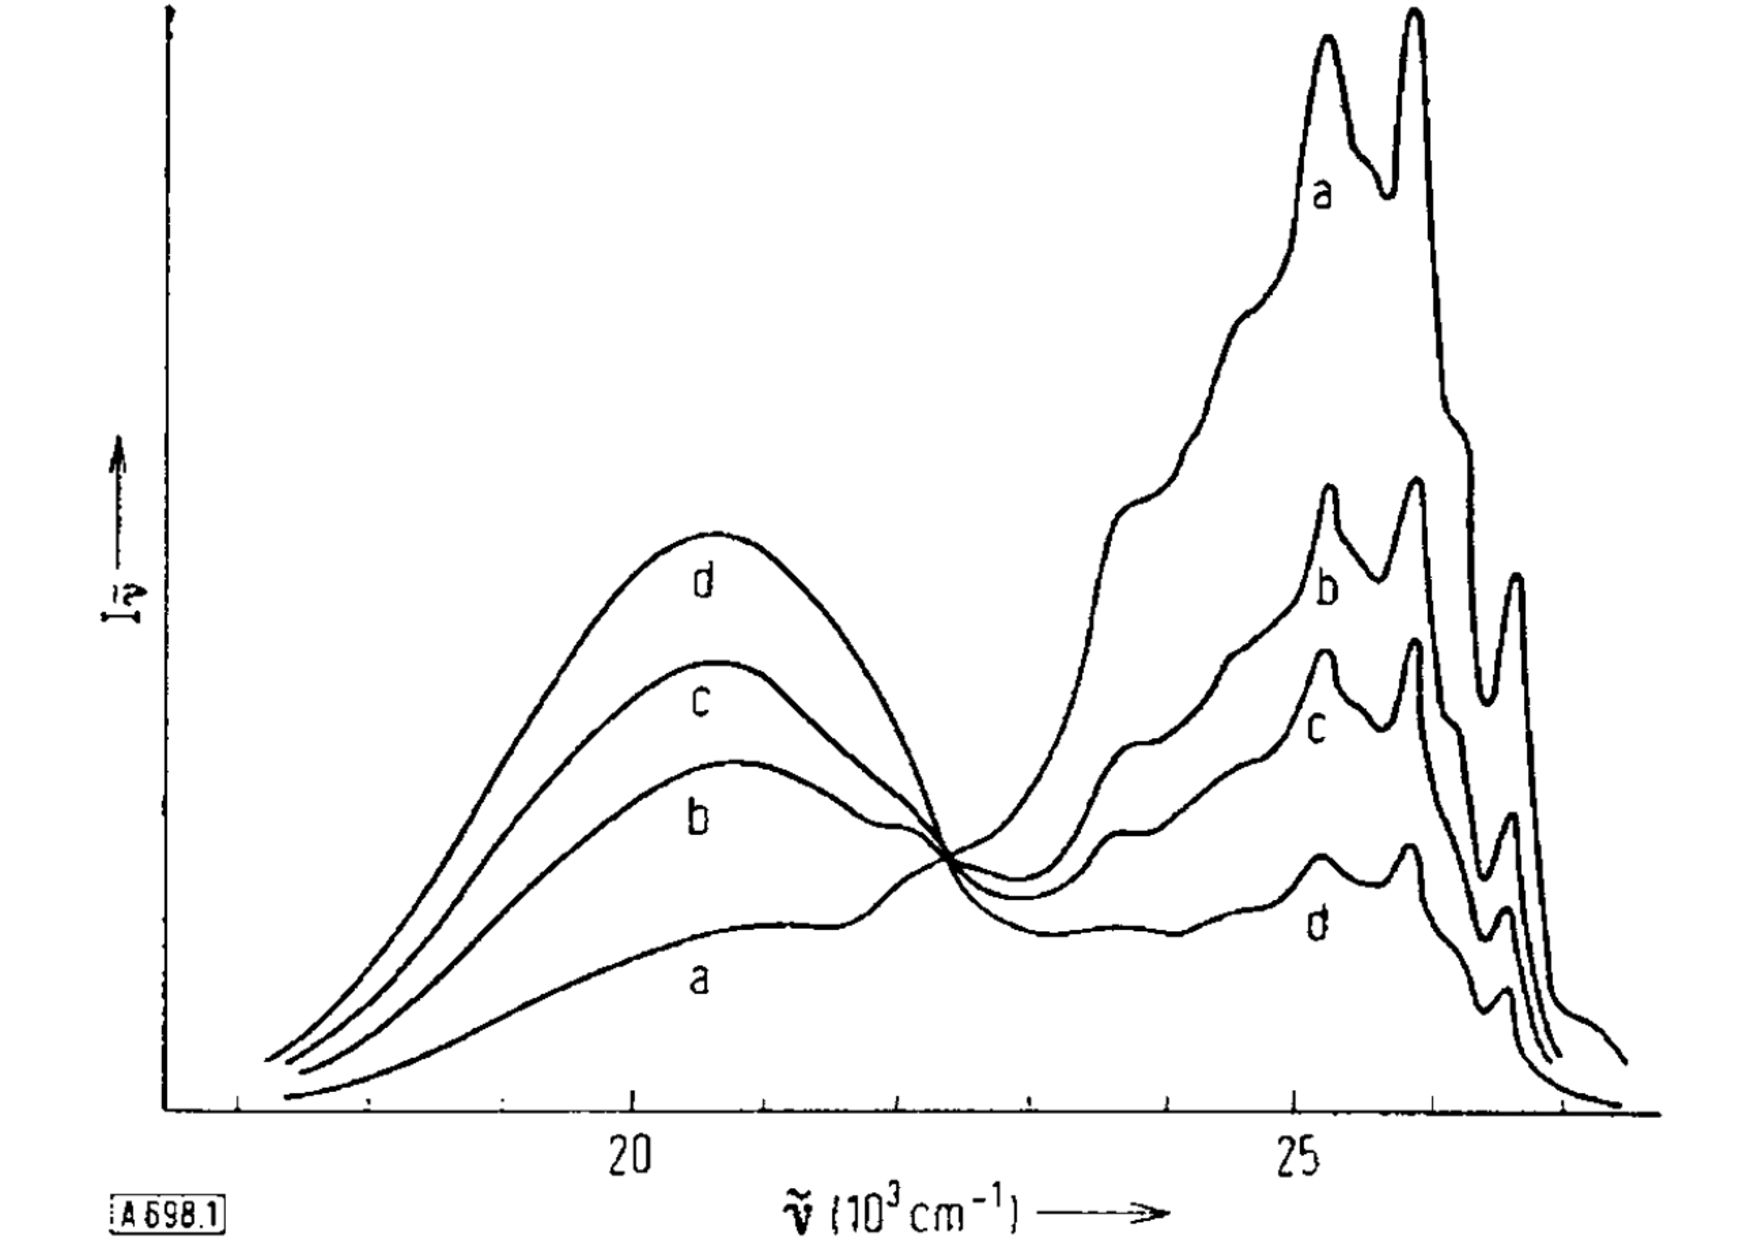
\includegraphics[width=0.6\linewidth]{1Intro/Forster_Spectra.pdf}
  \caption[Fluorescence spectrum of pyrene]{Fluorescence spectrum of pyrene (in n-heptane, 20\degree{}C) at different concentrations: a) \SI{5.0e-5}, b) \SI{1.8e-4}, c) \SI{3.1e-4}, d) \SI{7.0e-4}{mol L^{-1}}. Reprinted from ref.~\citenum{Forster1969} with permission of Wiley-VCH.}
  \label{figure: Forster_Spectra}
\end{figure}
The supermolecular alignment of aromatic groups is commonly termed $\pi$-stacking or $\pi$-$\pi$ interactions in the chemical literature. However, this labelling can be slightly misleading and even inaccurate.\cite{Grimme2008,Martinez2012} Stefan Grimme argues that a specific $\pi$-$\pi$ interaction arises only in large, polyaromatic groups as a result of increased dispersion in specific orientations.\cite{Grimme2008} Meanwhile, a thorough review of experimental and theoretical literature by Martinez and Iverson found a lack of the face-centred stacking of aromatic groups which would maximise overlap of aromatic $\pi$ clouds.\cite{Martinez2012} They argue that the terms $\pi$-stacking and $\pi$-$\pi$ interactions are misnomers since they incorrectly imply the ubiquity of face-face stacking motifs. Typical stacking motifs are shown in Figure \ref{figure: Benzene_Stacking}, where parallel displacement tempers the unfavourable electrostatic interaction and reduces the Pauli exchange repulsion, with the dominating factor being the favourable dispersion interaction. Inclusion of substituents introduces a permanent dipole, with substituents preferentially aligning antiparallel.\cite{Martinez2012}

\begin{figure}[H]
\centering
  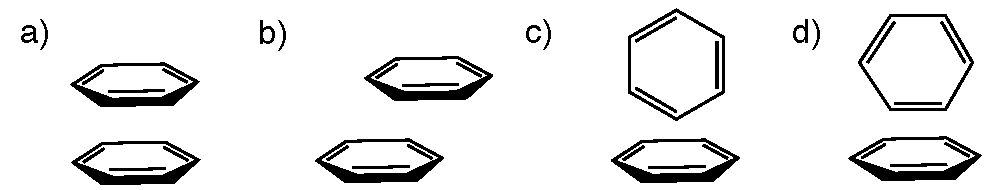
\includegraphics[width=0.7\linewidth]{1Intro/Stacking.pdf}
  \caption[Stacking motifs of benzene]{Packing motifs of benzene molecules: a) face-centred, b) displaced, c) Perpendicular T-shaped, d) Perpendicular Y-shaped. Adapted from ref.~\citenum{Martinez2012}.}
  \label{figure: Benzene_Stacking}
\end{figure}

This intermolecular interaction is detrimental to solid-state fluorescence, and yet is a direct consequence of the design requirements of the chromophore. In biosensing applications, researchers resorted to using dilute solutions with reduced sensitivity because of \ac{ACQ}.\cite{Thomas2007,Kwok2015} In the solid state, for instance in thin films for optoelectronics, the \ac{ACQ} effect means that solution screening for viable candidates is rendered meaningless by the differing luminescent properties of the final material compared to the molecule. Strategies to circumvent \ac{ACQ} have seen varying success, for example through the inclusion of bulky substituents, polar groups, and promotion of hydrogen bonding.\cite{Hong2009,Zhang2013,Mei2014,Mei2015} However, synthetic modification can in turn affect the chromophore's electronic structure and its excited state properties, thus commencing a tedious trail-and-error optimisation process. Attempts to physically block aggregation by encapsulating in surfactants or polymer matrices require extensive engineering and can reduce charge transport.\cite{Hong2009,Chen2000,Lee2013} 

The deleterious effects of \ac{ACQ} cannot be underestimated and pose a significant problem for organic luminescent applications. In the next section of this chapter, we shall look in more detail of the photophysics of molecular aggregates, within the context of Kasha's exciton theory.
%%%%%%%%%%%%%%%%%%%%%%%%%%%%%%
\subsection{Photophysics of Molecular Aggregates}\label{section: lom intermolecular-interactions}
Intermolecular interactions become photophysically important in the solid state due to the dense packing of molecular units. This effect is typically framed in Kasha's two state exciton theory.\cite{Gierschner2009,Gierschner2013,Gierschner2013a,Hestand2017,Shi2017} The exciton is typically defined as a deloclised excited state, where the excited electron and hole remain in close proximity. The Coulomb interaction between the transition dipoles of the monomers in a dimer results in an energy shift in the absorption spectrum, and has underpinned exciton theory since its inception in the 1960s.\cite{Kasha1965a} When two monomers stack ``side-by-side", the Coulombic electronic coupling is positive, a blue-shifted absorption spectrum is witnessed (relative to the isolated monomer) and radiative decay is reduced. This stacking motif is denoted a H-aggregate. Conversely, in J-aggreagtes, dimers align ``head-to-tail", and a red-shifted absorption is witnessed with an increased radiative decay. These extreme cases have helped interpret the supermolecular photophenomena in molecular aggregates.

When the intermolecular distance is large enough to prevent orbital overlap, the exciton can be considered as the interaction of the wavefunction of one monomer ($\ket{1}$) with the wavefunction of the second monomer ($\ket{2}$). In the excited state, the  wavefunctions interact to form a delocalised exciton (a Frenkel exciton), the Hamiltonian $H$ of which is given
\begin{equation}
H=\hbar\omega + \mathrm{\hbar{}D} + J_{0}\{\ket{1}\bra{2}+\ket{2}\bra{1}\}.
\end{equation}
The first term is the energy gap between S\textsubscript{0} and S\textsubscript{1},  $\hbar{}D$ is the shift of the S\textsubscript{1} state in going from the vacuum to the crystal, and $J_{0}$ is the Coulombic coupling.\cite{Spano} The exciton for a multisite system can be described using periodic boundary conditions to produce a wavelike function $k$. For the two site system, $\ket{k}$ is\cite{Hestand2018}
\begin{equation}
\ket{k}=\frac{1}{\sqrt{2}}\big[e^{ik}\ket{1}+  e^{i2k}\ket{2}\big]\qquad\quad k=0,\pm{\pi}.
\end{equation}
For the allowed values of $k$, the transition energy $E_k$ for state $k$ is an eigenvalue of $H$, and has the form
\begin{equation}
\mathrm{E}_{k}=\hbar\omega + \mathrm{\hbar{}D} +J_{0}\cos{k}.
\end{equation}
For the two site system, this results in two exciton states in the Frenkel Hamiltonian, as depicted in Figure \ref{figure: H_J_Aggregates}. The Coulomb coupling $J_{0}$ represents the interaction energy due to exchange of excitation energy between $\ket{1}$ and $\ket{2}$, the sign of which dictates whether the symmetric superposition is the upper or lower state. When the coupling is positive, the symmetric state is the upper state, as in the H-aggregate, and the transition dipoles are reinforced resulting in absorption is blue-shifted compared to the gas-phase monomer. Since emission usually takes place from the lower state, where transition dipoles moments cancel, the state is nonradiative and fluorescence is quenched. When the coupling is negative, the symmetric state is lowered and emission is symmetry allowed.\cite{Hestand2017}
\begin{figure}[H]
\centering
  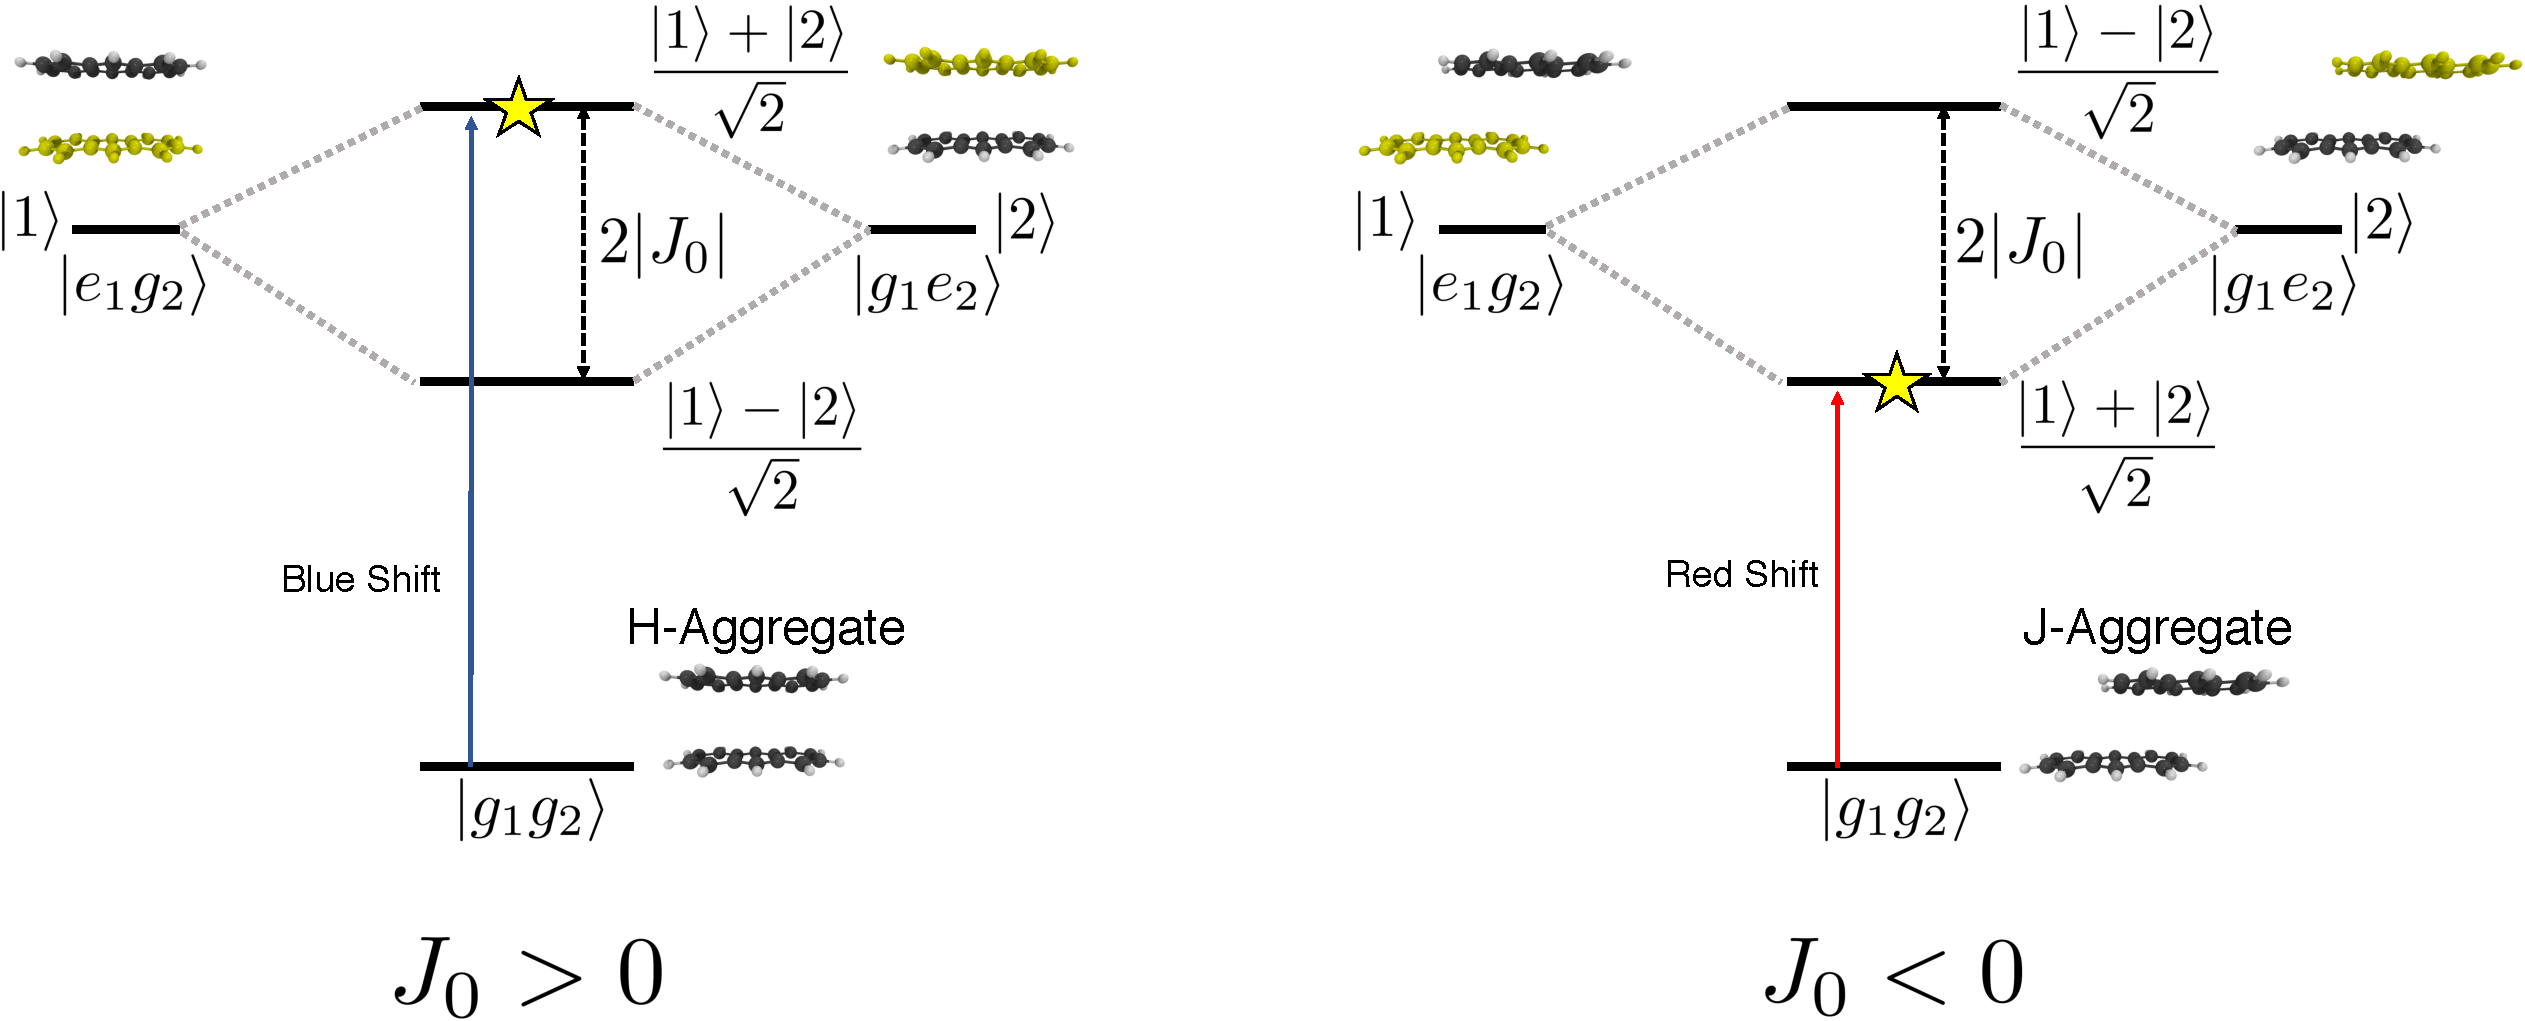
\includegraphics[width=\linewidth]{1Intro/H_J_aggregates.pdf}
  \caption[Exciton energy level diagram for H- and J-aggregates]{Energy level diagram for a H-aggregate (left) and J-aggregate (right) of naphthalene. For the H-aggrgate, the Coulombic coupling $J_{0}$ is positive, raising the energy of the symmetric state resulting in blue-shifted absorption with respect to the monomer state. Emission from the lower state is forbidden, and thus quenched. In the J-aggregate, the negative Coulombic coupling results in red-shifted absorption and allowed emission. The bright excitonic state, the symmetric superposition of the monomer wavefunctions, is indicated with a star.}
  \label{figure: H_J_Aggregates}
\end{figure}
\begin{comment}
\begin{equation}
\ket{g_{1}g_{2}}
\end{equation}
\begin{equation}
\ket{e_{1}g_{2}}
\end{equation}
\begin{equation}
\ket{g_{1}e_{2}}
\end{equation}
\begin{equation}
J_{0}>0
\end{equation}
\begin{equation}
J_{0}<0
\end{equation}
\begin{equation}
2|J_{0}|
\end{equation}
\begin{equation}
\frac{\ket{1}+\ket{2}}{\sqrt{2}}
\end{equation}
\begin{equation}
\frac{\ket{1}-\ket{2}}{\sqrt{2}}
\end{equation}
\begin{equation}
\ket{1}
\end{equation}
\begin{equation}
\ket{2}
\end{equation}
\end{comment}
H- and J-aggregates represent the two extreme stacking cases. In Kasha's theory, the coupling $J_{0}$ arises from the interaction of the transition dipole moments, which at its most crude can be treated as the interaction between two point dipoles,
\begin{equation}
    J_{0,Coul}=\frac{\mu^{2}(1-3\cos^{2}\theta)}{4\pi\epsilon{}R^3}
\end{equation}
where $R$ is the intermolecular distance (between the centroids of the monomers), $\theta$ is the angle between  $\bm{\mu}$ (transition dipole vector) and $\bm{R}$, and $\epsilon$ is the optical dielectric constant of the medium. Thus for H-aggregates, when $\theta$=90\degree{}, the coupling is positive, and is negative in J-aggregates when $\theta$ is close to zero. H-aggregates become J-aggregates at the so-called ``magic angle" of 54.7\textdegree.\cite{Hestand2018}

The crude point-dipole, Coulomb interpretation of the coupling is only valid approximation for homodimers with large intermolecular separation.\cite{Kistler2013} When monomers stack in close proximity ($R\leq4\si{\angstrom}$), wavefunction overlap invokes the possibility of \ac{CT} states, where the electron resides on one site and the hole on another.\cite{Darghouth2018} This creates a short-range coupling factor as well as the long-range Coulomb coupling. The total coupling is the combined short-range \ac{CT} coupling and the Coulomb coupling, leading to complex behaviour which is dependent on the sign of the short- and long-range contributions. For example, the \ac{CT} coupling is highly sensitive to the molecular geometry, where small distortions can change the total coupling value and result in multiple H- to J-aggregate conversions.\cite{Arago2015} The two components of the total coupling has lead to an expanded nomenclature for stacking motifs, where the contribution of both the short and long-range coupling is considered (HH, HJ, JH, JJ). In the JH and HJ, the interference is completely destructive and the total coupling is zero, resulting in an absorption spectrum at the same position as a monomer.\cite{Hestand2017}

Understanding the complex photophenomena of molecular aggregates is important in the development of materials requiring control over the exciton. The existence of excitons and the dynamics in the solid state, opens nonradiative decay channels and often a quenching of fluorescence for typical aromatic motifs. This has hindered the development of solid-state organic lumniscence. However, when the group of Ben Zhong Tang found a system which had its fluorescence switched on, rather than quenched, upon aggregation, a new strategy for the design and development of brightly luminescent organic materials was launched. They named the phenomenon \acf{AIE}. In the next section of this chapter, the roots of \ac{AIE} shall be examined and the technological advances that have arisen from the discovery briefly outlined.

%%%%%%%%%%%%%%%%%%%%%%%%%%%%%%
%%%%%%%%%%%%%%%%%%%%%%%%%%%%%%
\section{Aggregation Induced Emission}\label{section: lom AIE}
%%%%%%%%%%%%%%%%%%%%%%%%%%%%%%
\subsection{Overview}
In 2001, the Tang group at the Hong Kong University of Science and Technology were interested in silole-based polymers for highly emissive thin-films. As was common at the time, fabrication of such materials was challenging due to \ac{ACQ}. Through serendipity during a purification process, they found that a wet spot of 1-methyl-1,2,3,4,5-pentaphenylsilole was almost non-emissive, but brightly fluorescent after solvent evaporation.\cite{Luo2001} The law of aggregation quenching emission had been turned on its head, and the Tang group had observed the exact opposite behaviour, of molecular aggregation inducing light emission. This was almost unheard of for small organic molecules. 

The Tang group used the \ac{AIE} phenomeon to develop a range of chemical sensors to detect for instance volatile organic compounds, explosives, and pH.\cite{Dong2007,Li2005,Li2009} Such was the magnitude of the \ac{AIE} breakthrough and the mechanistic interpretations provided by the Tang group, many other groups began to explore this exciting new phenomenon for a wide range of applications. In the field of biological probing, \ac{AIE}-active systems can detect important small molecules such as glucose, thiols, and lactic acid.\cite{Wang2014,Yuan2014,Shen2012} Probes have been developed to detect protein fibrillation, which has been linked to Alzheimer's, Parkinson's and type II diabetes.\cite{Hong2012} \ac{AIE} systems have been also used in medical imaging, where fluorescence is an attractive technique due its high resolution, wide applicability, and low cost.\cite{Mei2015} The Tang group have tracked the progress of the field with periodic, in-depth reviews of the vast number of innovations, of which they contribute a significant share.\cite{Hong2009,Wang2010a,Hong2011,Mei2014,Hu2014,Mei2015} The most prominent avenue for the application of AIE is in optoelectronic and lasing devices, particularly OLEDs, which we will overview in the next section. 
\subsection{Optoelectronic Applications of AIE}
Upon discovery of \ac{AIE}, the potential for the improvement of optoelectronic devices was immediately apparent. In the original publication, the group built a highly emissive blue-emitting electroluminescent device, and optimised the device to 8\% \ac{EQE} in the cyan region, a vast improvement on the previous high of just 1.5\% for an \ac{OLED}. \cite{Luo2001,Chen2002} \ac{EQE} is the product of the electroluminescence efficiency of the emitter (the organic layer in this case) and the external coupling factor, which is a measure of the fraction of light able to escape the \ac{OLED}. Due to electroluminescence efficiency being limited to 25\% for singlet emitters, and the external coupling being limited to around 22\%, it was previously thought that the theoretical maximum \ac{EQE} is 5.5\%. Indeed, such was the remarkable \ac{EQE} measure in this \ac{OLED} that these previously accepted limitations had to be reconsidered.

In follow-up work, a light-blue emitting \ac{OLED} with hexaphenylsilole (Figure \ref{figure: HPS_TPE}) as the emitting layer was fabricated with \ac{EQE} of 7\%.\cite{Chen2003} While the unfavourable spin statistics inhibit efficiency for singlet-emitting \acp{OLED} across the visible spectrum, deep blue emitters are harder still since the large band gap makes charge injection difficult, hindering the development of full colour displays. Non-doped deep blue \acp{OLED} with \ac{EQE} of around 4\% were reached in 2014, with emitters based on triphenylamine and tetraphenylethene (Figure \ref{figure: HPS_TPE}).\cite{Huang2014,Huang2014a} This has recently been increased to 6.5\% using a carbazole-based organic layer, and in 2018 reached 9.4\%.\cite{KumarKonidena2017,Tang2018} This represents a high for non-doped singlet blue emitters. Inclusion of phosphorescent or thermally-activated delayed fluorescent dopants can further increase the quantum efficiency by harvesting triplet states for luminescence.\cite{Zhu2018}

\begin{figure}[H]
\centering
  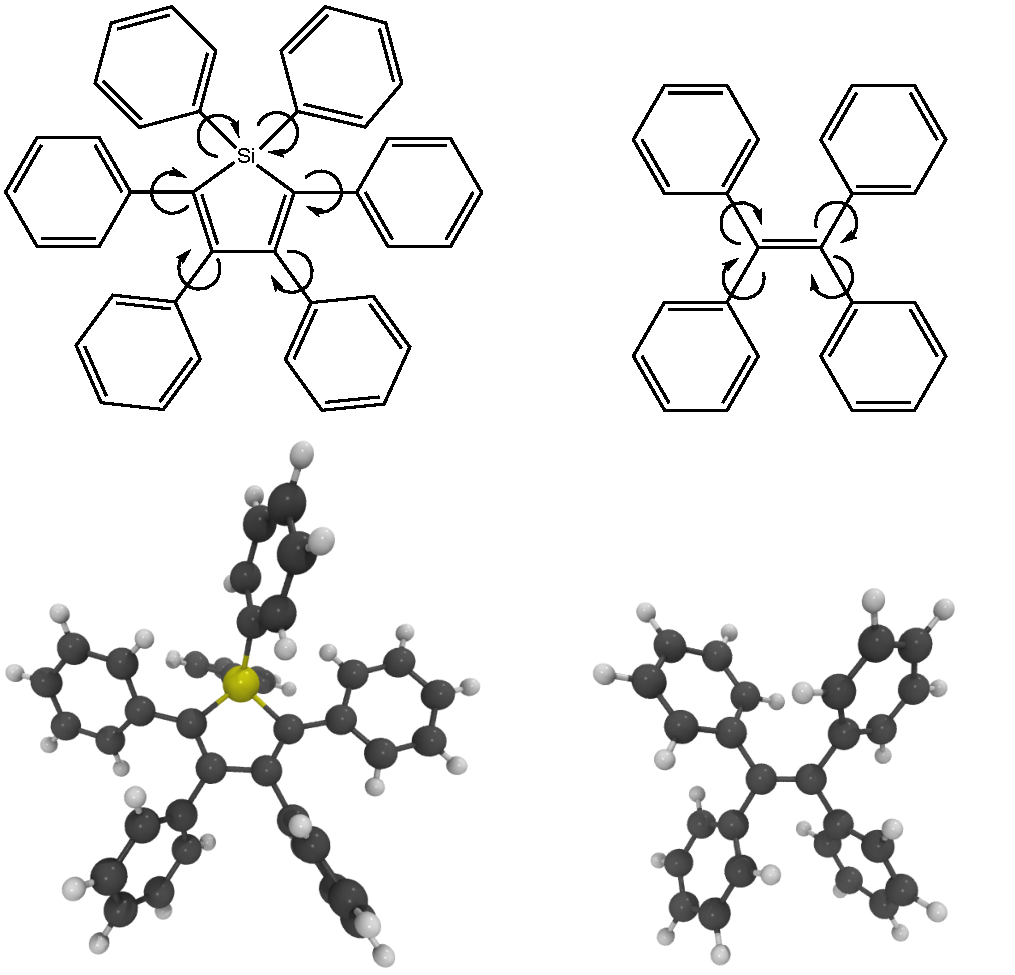
\includegraphics[width=0.7\linewidth]{1Intro/HPS_TPE.pdf}
  \caption[Examples of AIE-active chromophores]{Two dimensional (top) and three dimensional (bottom) structures of two of the ubiquitous AIE-active systems, hexaphenylsilole (HPS, left) and tetraphenylethene (\ac{TPE}, right). AIE occurs through restriction of the rotational motions depicted with arrows.}
  \label{figure: HPS_TPE}
\end{figure}
\subsection{Hypothesised Mechanisms}
Systems exhibiting \ac{AIE} are typically based on a propeller architecture, where a central stator is connected to a number of aromatic rotors via single bonds, as shown in Figure \ref{figure: HPS_TPE}. In the initial analysis of 1-methyl-1,2,3,4,5-pentaphenylsilole, the absorption spectra showed that after the water fraction in an ethanol-water solvent mixture rose above 60\%, the absorption band increased in intensity and moved to longer wavelengths.\cite{Luo2001} On this basis, the \ac{AIE} activity was attributed to the formation of aggregates which forced the molecules into a more planar conformation, thus increasing the conjugation and the absorption. Enough rotation about the sigma bonds was still possible to prevent complete planarity and therefore limiting the stacking and subsequent fluorescence quenching. 

A few months later, the group showed the \ac{AIE} effect for four more silole systems, followed by an extensive study of ten phenylsiloles.\cite{Tang2001,Chen2003} Crucially, in this later work the crystal structure of the siloles showed that the conformation remains twisted in the solid state.\cite{Chen2003} Large torsional angles exist between the phenyl groups and the central silole moiety, on account of the steric repulsion between the six phenyl groups. The lack of space between the phenyl blades, and their angular orientations, prevents intermolecular stacking which give rise to aggregation caused quenching. Therefore the planarisation hypothesis was wrong. 

The group investigated other quenching mechanisms, such as \ac{TICT}, where a non-emissive twisted conformer is formed via charge separation in the chromophore. The \ac{TICT} state can be stabilised, and thus favoured, in polar solvents. However, no emission was recorded across a wide range of solvent polarities for the siloles, ruling out \ac{TICT} as the cause for \ac{AIE}. Also, the lack of electron donor and acceptor groups make it highly unlikely that \ac{TICT} could take place in the siloles. In an elegant experiment it was found that the emission increased almost linearly with increasing solvent viscosity, even though no aggregates were formed. In a similar vain, the photoluminescence intensity increased with decreasing temperature, with NMR studies confirming that the intramolecular rotations of the exterior phenyl groups were reduced at lower temperatures. It was concluded the in good solvents, at ambient temperature, the energy consumed by the rotation of the phenyl groups about the single bonds results in the nonradiative decay of the excited state decay. Upon aggregation, the propeller-like shape limits the intermolecular stacking. Strong C-H\textperiodcentered\textperiodcentered\textperiodcentered$\pi$ interactions rigidify the structure, hindering the intramolecular rotation and the excited state decays via fluorescence.\cite{Chen2003}

The \ac{RIR} mechanism allowed the library of \ac{AIE}-active systems to be expanded to other molecules with propeller-shaped structures. Along with the phenylsiloles, \ac{TPE} derivatives (Figure \ref{figure: HPS_TPE}) have driven understanding and technological progress in the field.\cite{Hong2009,Wang2010a,Hong2011,Mei2014,Hu2014,Mei2015} By switching a phenyl group of \ac{TPE} with a traditional \ac{ACQ} molecules, such as triphenylamine or carbazole, the electroluminscence properties of the system are enhanced due to the hole-transport properties of the \ac{ACQ} group.\cite{Chan2014} Conversely, \ac{ACQ} cores can be made to undergo \ac{AIE} by the attachment of \ac{TPE}.\cite{Yuan2010a}

Dissipation of the excited state can occur through means other than rotation. A bent, $\pi$-surface system of benzenes fused with cyclooctatetraenes undergoes \ac{AIE} but without any rotable units.\cite{Nishiuchi2013} In solution, ring inversions dissipate the excited state and there is almost no emission. Single crystals show emission in the blue region, since the bent structure prevents facial stacking and the inversion modes are restricted. Thus \ac{AIE} is achieved through \ac{RIV}. In a similar vain, the \ac{RIV} mechanism can be applied to \ac{TPE} by locking pairs of phenyl groups with eythlene linkers. In 2014, Tang unified the \ac{RIR} and \ac{RIV} interpretations under the \ac{RIM} umbrella.\cite{Leung2014}

The discovery and development of the \ac{AIE} phenomenon has transformed the field of luminescent organic materials. While much of the innovation has been based on the propeller systems, a class of systems based on \ac{ESIPT} have attracted interest in recent years for their favourable photochemical properties. \ac{ESIPT} systems form the basis of the research in this thesis and in the next section the \ac{ESIPT} mechanism shall be introduced, along with the key applications which incorporate \ac{ESIPT}.
%%%%%%%%%%%%%%%%%%%%%%%%%%%%%%
\section{Theoretical Framework }\label{section: lom theory}
%%%%%%%%%%%%%%%%%%%%%%%%%%%%%%
%%%%%%%%%%%%%%%%%%%%%%%%%%%%%%
\subsection{Approaches Based on Fermi Golden Rule}\label{section: lom FGR}
%%%%%%%%%%%%%%%%%%%%%%%%%%%%%%
In 2005, the first theoretical study for the root of AIE in the phenylsiloles was presented, led by the group of Zhigang Shuai.\cite{Yui2005} To probe the origins of the AIE phenomenon, calculated the rates of the excited state decay processes and constructed a model for the observed \ac{QE} of photoluminescence, $\Phi_{\mathrm{PL}}$, 
\begin{equation}\label{equation: QE}
    \Phi_{\mathrm{PL}}=\frac{k_{r}}{k_{r}+k_{nr}}
\end{equation}
where the overall observed \ac{QE} is determined by the rates of radiative ($k_{r}$) and nonradiative ($k_{nr}$) decay. $k_{nr}$ will typically consist of internal conversion, intersystem crossing, and intermolecular processes such as charge transfer. The idea is to determine the radiative and nonradiative rates in solution and aggregate form to elucidate the reason for the increased fluorescence in the solid state. This strategy underpins most of the theoretical work into AIE, of which the Shuai group have been at the forefront over the last 10-15 years. 

To evaluate $k_{r}$, the Einstein spontaneous emission formula can be applied,
\begin{equation}
    k_{r}=\frac{fE_{if}^{2}}{1.499}
\end{equation}
where $f_{if}$ is the oscillator strength and $E_{if}$ is the energy difference between the initial (\sone{}) and final electronic state (\szero{}). This considers that there is no displacement between the ground and excited state \acp{PES}. A more realistic method to evaluate $k_{r}$ is to simulate the fluorescence spectrum using a Winger ensemble and integrate the spontaneous emission for the rate.\cite{Crespo-Otero2012} Calculating $k_{nr}$ for internal conversion is an altogether more challenging prospect, since both electronic and vibrational wavefunctions must be considered. The Fermi Golden rule and Condon approximation can be used within the Born-Oppenheimer approximation to determine $k_{nr}$ according to
\begin{equation}\label{equation: Fermi}
    k_{nr}(T)=\frac{2\pi}{\hbar}\sum_{\nu_{i}\nu_{f}}P_{i\nu_{i}}(T)\bigg|\sum_{k}\bra{\Phi_{f}}\hat{P}_{k}\ket{\Phi_{i}}\bra{\Theta_{f\nu_{f}}}\hat{P}_{k}\ket{\Theta_{i\nu_{i}}}\bigg|^{2}\delta{}(E_{i\nu_{i}}-E_{f\nu_{f}})
\end{equation}
where $P$ is the Boltzmann distribution of vibrational states ($\nu$) in the initial electronic state ($\Phi_{i}$), $\hat{P}$ is the momentum operator to give the coupling between electronic states and nuclear ($\Theta$) wavefunctions. The first sum runs over each of the vibrational states in the initial ($\nu_{i}$) and final ($\nu_{f}$)  states, and Boltzmann probability for the excited state (($\nu_{i}$) is multiplied by the product of the electronic (or nonadiabatic) coupling and the vibrational coupling. The coupling terms measure the change of the nuclear and electronic wavefunctions due to nuclear displacements for each nuclei $k$. For systems with small spin-orbit coupling, the contributions of intersystem crossing are normally neglected. As such, the framework for evaluating $k_{nr}$ focuses on internal conversion processes, although intermolecular decay through exciton formation or charge transfer are of growing interest.\cite{Li2017} 

Solving Equation \ref{equation: Fermi} is computationally demanding and thus approximations must be made. Initially Shuai \textit{et. al.} used a displaced harmonic approximation, where it is assumed that the excited state \ac{PES} is just a rigid displacement of the ground state.\cite{Yui2005} The internal conversion rate can then be racast as
\begin{equation} \label{equation: displaced_harmonic}
    k_{nr}=\sum_{l}\frac{1}{\hbar}\bigg[\frac{\omega_{l}}{2\hbar{}}\big|R_{fi}^{l}\big|^{2}\bigg]N_{FC}
\end{equation}
where $R^{l}_{fi}$ are the nonadiabatic couplings, $\omega_{l}$ is the frequency of mode $l$ and $N_{FC}$ is the density-weighted Franck-Condon factor, given by
\begin{equation}\label{equation: NFC}
N_{FC}=\sqrt{\frac{2\pi}{\sum_{j}S_{j}\omega^{2}_{j}(2\bar{n}_{j}+1)}}\mathrm{exp}\bigg[-\frac{(\omega_{fi}+\omega_{l}+\sum_{j}S_{j}\omega_{j})^{2}}{2\sum_{j}S_{j}\omega_{j}^{2}(2\bar{n}_{j}+1)}\bigg].
\end{equation}
$k_{nr}$ the weighted Franck-Condon factors are functions of the \ac{HR} factors $S$ for each mode $j$, which determine the difference in vibrational wavefunctions in different electronic states. One of the main parameters obtained from the \ac{HR} factors is the reorganization energy $\lambda$ for each vibrational mode \textit{via},
\begin{equation}
    \lambda_{j}=\hbar{}S_{j}\omega_{j}
\end{equation}
which is associated with the energetic cost of geometry relaxation in the electronic transition. Analysis of $S_{j}$, $\sum_{j}\lambda_{j}$ and the nonadiabatic couplings give insight into the main vibrational modes involved in the internal conversion. In particular, analysis of the HR factors and reorganisation energies are popular for the semi-quantitative interpretation of AIE.\cite{Yin2006,Peng2007,Li2011,Peng2013,Shuai2014c,Shuai2014,Wu2014,Zhang2015a,Zheng2016,Fan2016,Zhang2016,Duan2017,Fan2017,Fan2018} Since $k_{nr}$ is a product of the electronic couplings and the Franck-Condon factors, both of these must be small in order to increase the QE (Equation \ref{equation: QE}). For the phenylsilole compounds, calculation of $k_{r}$ and $k_{nr}$ in vacuum and the solid state revealed that the most significant contributions to $k_{nr}$ come from low-frequency rotational modes, which have large \ac{HR} factors and large reorganisation energies. While the radiative decay rate remains relatively similar, in vacuum $k_{nr}$ is three orders of magnitude larger than $k_{r}$. The authors hypothesise that in the solid state, the dampening of rotational  modes due to steric hindrance reduces the \ac{HR} factor, and thus the $N_{FC}$ contribution to $k_{nr}$.\cite{Yui2005,Yin2006} $k_{nr}$ decreases with respect to $k_{r}$, resulting in fluorescence.

Within the displaced harmonic oscillator model (Equation \ref{equation: displaced_harmonic}), some key approximations are made. Firstly, by assuming the ground and excited state \acp{PES} mirror each other means that the model is only valid for systems where the excited state geometry does not deviate far from the ground state equilibrium position. Secondly, in the implementation a ''promoting-mode" $l$ is chosen which is used to calculate the nonadiabatic coupling but does not contribute to $N_{FC}$ (Equation \ref{equation: NFC}). This is chosen manually. 

To overcome these limitations, Shuai \textit{et. al.} further developed the theory to incorporate the \ac{DRE}, such that all vibrations are considered rather than just one promoting mode.\cite{Yui2005,Peng2007a,Niu2010}. The \ac{DRE} correlates the excited state coordinates $Q^{e}$ with those of the ground state $Q^{e}$
\begin{equation}
    Q^{e}_{i}=\sum_{j}S_{ij}Q^{g}_{j}+D_{i}
\end{equation}
where $S$ is the Duschinsky rotation matrix and $D_{i}$ is the displacement of the two \ac{PES}. Inclusion of \ac{DRE} involves solving Equation \ref{equation: Fermi} through a path-integral formalism. Fourier transform of the delta function yields the thermal vibrational correlation function which can be solved analytically \textit{via} the implementation of Peng and Shuai.\cite{Peng2013}
%\begin{equation}
%k_{nr}=\sum_{kl}\frac{1}{\hbar}R_{kl}\int_{\infty}^{\infty}\%diff{t}\big[e^{i\omega_{if}t}Z_{i}^{-1}\rho_{IC}(t,T)\big]
%\end{equation}
Incorporating \ac{DRE} to model the effect of temperature shows that increases $k_{nr}$ by 700 times when the temperature increases from 70K to 300K.\cite{Peng2007} Low-frequency modes are strongly coupled for tetraphenyl butadiene compounds, while high-frequency modes are less sensitive to temperature effects and less affected by \ac{DRE}. 

Shuai \textit{et. al.} have also considered the effect of including exciton couplings in nonradiative decay rates.\cite{Li2017} The authors developed an analytical expression for $k_{r}$ incorporating the exciton coupling and evaluated the decay rates for four aromatic molecules and four typical AIE chromophores. It was found that the the exciton coupling increases $k_{r}$, but only slightly. The values of exciton couplings for the tested systems was less than 30meV, which is relatively small.

The framework developed by Shuai group have made major progress in rationalising AIE through the restriction of intramolecular motions interpretation. The group have implemented the methods in a closed-source, commercial code MOMAP.\cite{Niu2018} However, the formalism contains some key approximations which should be highlighted. For the electronic nonadiabatic coupling, perturbation theory is used where the magnitude of the coupling is only calculated at the equilibrium geometries in \szero{} and \sone{}. This may be a source of error in systems which deviate from the equilibrium structures, as nonadiabatic couplings can vary significantly in the regions of surface crossings. Further, low-frequency modes driving the photochemistry can be highly anharmonic and nonadiabatic couplings in the equilibrium region do not necessarily correlate with the deactivation modes driving the photochemistry. In general, the use of the harmonic potentials potentially limits the applications to molecules which excited state dynamics is restricted to regions of the PES around equilibrium. These approximations can break down in systems with more highly anharmonic excited state \acp{PES}. 
%%%%%%%%%%%%%%%
%%%%%%%%%%%%%%%
\subsection{Restriced Access to Conical Intersection Model}\label{section: lom RACI}
%%%%%%%%%%%%%%%
%%%%%%%%%%%%%%%
A different approach to computational modelling of AIE is to consider the topology of the whole \ac{PES} across the photochemical reaction coordinate. While the framework adopted by Shuai considers the vibronic coupling around the equilibrium geometries, insight into the AIE mechanism can be found by considering the role of conical intersections. Conical intersections are points of degeneracy between electronic states, and allow for nonadiabatic radiationless decay between an upper and lower surface. A more detailed overview on conical intersections is given in Chapter \ref{section: Photo}. In the \ac{RACI} model of Blancafort \textit{et. al.}, an energetically accessible conical intersection is responbsible for the nonemission in solution. Upon aggregation, steric constraints result in the conical intersection being too high in energy to be populated, leading to fluorescence.\cite{Peng2016} The \ac{RACI} is advantageous in that it does not impose restrictions or assumptions of the topology of the \ac{PES}.  

Blancafort and co-workers first identified the role of a conical intersection for systems based on diphenyldibenzofulvene using multiconfigurational methods.\cite{Li2013}. In solution, torsional rotation takes the system to an extended crossing seam, with the \ac{MECI} lying 0.7 eV below the excitation energy. In the crystal, rotation is hindered and the \ac{MECI} lies above the excitation energy. The role of the phenyl substituents in the RACI model is not as energy dissipators. Instead, they restrict the torsion in the solid state.   Wang \textit{et. al.} found a similar mechanism for 4-diethylamino-2 benzylidene malonic acid dimethyl ester. \cite{Wang2016} By combining TDDFT, CASSCF, and CASPT2 methods, the authors compared the \acp{PES} in solution and in the solid state. In solution, relaxation along a torsional mode takes the system to a conical intersection which is inaccessible in the crystal. A schematic of the \ac{RACI} mechanism is depicted in Figure \ref{figure: RACI}.

\begin{figure}[t]
\centering
  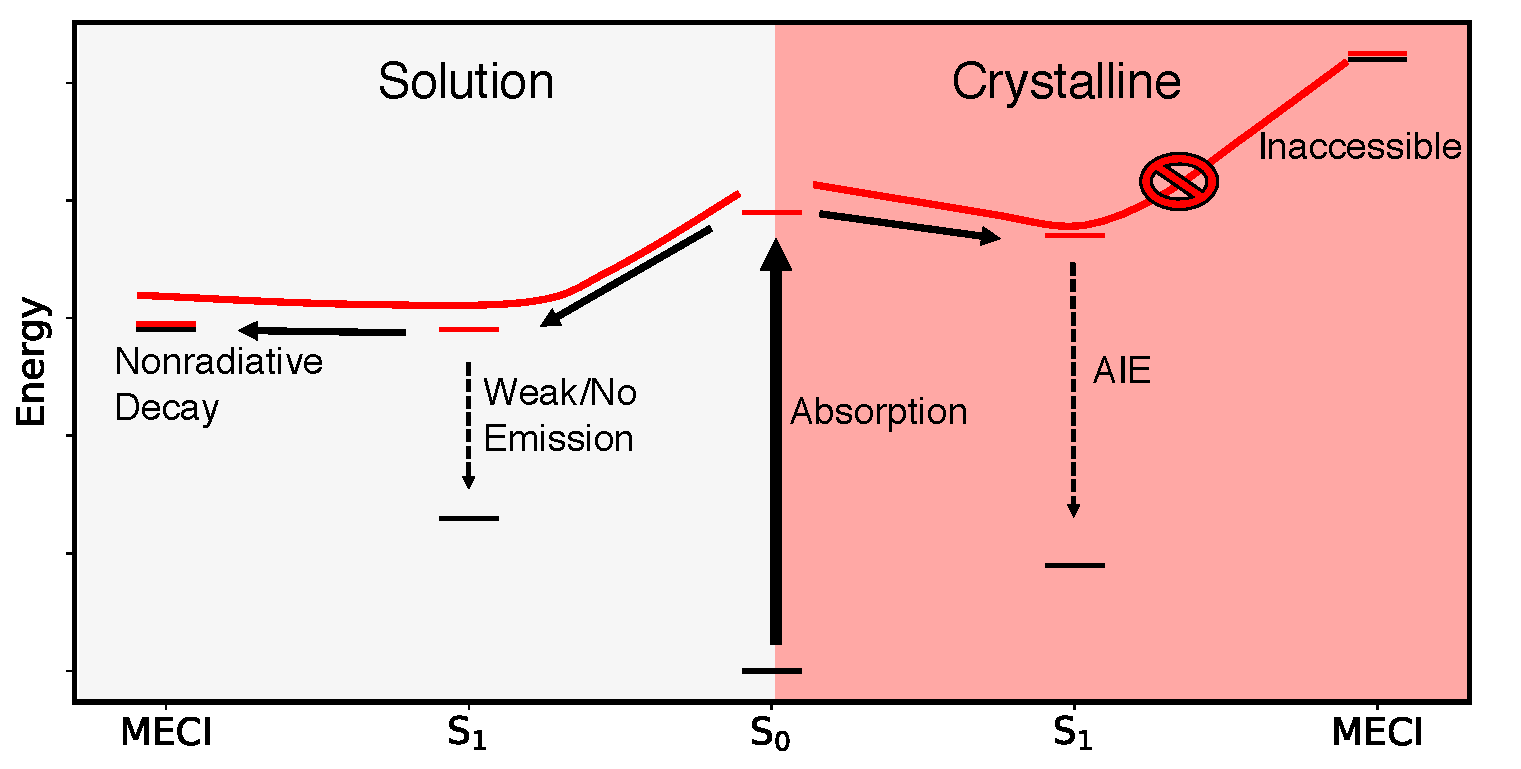
\includegraphics[width=0.9\linewidth]{1Intro/RACI_Model.pdf}
  \caption[Schematic of the RACI Model]{Schematic of the RACI model, where in solution there is no emission due to the energetically accessible conical intersection. In crystalline or aggregated state, the minimal energy conical intersection (MECI) is high in energy and inaccessible, which results in AIE.}
  \label{figure: RACI}
\end{figure}

The RACI model has also been applied to explain the different emissive responses of dicyano-distyrilbenzene derivatives with differing CN substituion patterns.\cite{Shi2017} For some derivatives, there is emission in both solution and the solid state, whereas others display AIE, due to the energetic accessibility of a CI in solution. In this case, it is the vertical excitation energy which is altered most between the compounds, with a red-shift making the conical intersection inaccessible. Again, the CI is reached through intramolecular rotation.

Studies have shown that modes other than rotation can be followed to access conical intersections. For \ac{TPE}, dynamics calculations at TDDFT level show that cylisation through bond formation can lead to nonradiative decay through a CI.\cite{Prlj2016} The formation of photocylisation products was later confirmed by transient absorption spectroscopy, while the methylated derivative of \ac{TPE} shows similar behaviour.\cite{Cai2018a,Gao2017} In Duan's study, it was proposed that nonradiative decay of a TPE derivative in solution could be on account of both the intermolecular motions and the conical intersection.\cite{Duan2017} 

Blancafort has shown that the RACI model can account for AIE in Tang's original compounds, the phenylsiloles.\cite{Peng2016} By combining TDDFT and CASSCF/CASPT2 calculations, it is found that a combination of ring puckering and a flapping mode result in a conical intersection in solution, which is inaccessible in the crystal. Ring puckering conical intersections have been found for other systems exhibiting AIE.\cite{Yuan2013,Sasaki2016}





%%%%%%%%%%%%%%%%%%%%%%%%%%%%%%
\section{Excited State Intramolecular Proton Transfer}\label{section: lom ESIPT}
%%%%%%%%%%%%%%%%%%%%%%%%%%%%%%
\subsection{Combining AIE with ESIPT}
Tautomerism is a type of isomerism resulting in the transfer of a chemical group between two sites on a molecule, and the simultaneous switching of a single and double bond. Photo-induced tautomerism, where the transferring group is a proton, is called \acf{ESIPT}. Research into the mechanism and potential applications of ESISPT has been active for more than half a century, since \ac{ESIPT} was first observed in the 1950s in salicylic acid. Photochromic materials harnessing \ac{ESIPT} have garnered much attention due to the wide range of applications and remarkable properties. In particular, it is the unusually large Stokes-shifted emission which makes \ac{ESIPT} so attractive. The separation between the absorption and emission bands can typically exceed 200 nm, reducing self-absorption and increasing the output signal for the desired application. The emission colour can be tuned by the addition of electron donating or withdrawing groups, as well as solvent polarity and viscosity.\cite{Azarias2016,Yushchenko2007} Dual emission from the pre- and post-\ac{ESIPT} forms is also possible. These characteristics, in tandem with \ac{AIE}, have resulted in \ac{ESIPT} chromophores being used for chemical sensing, biological imaging and probing, as well the optoelectronic applications such as optical memory, lasers, and \acp{OLED}.\cite{Hsieh2010,Kwon2011,Zhao2012,Demchenko2013,Padalkar2015,Chen2018}
\begin{figure}[H]
\centering
  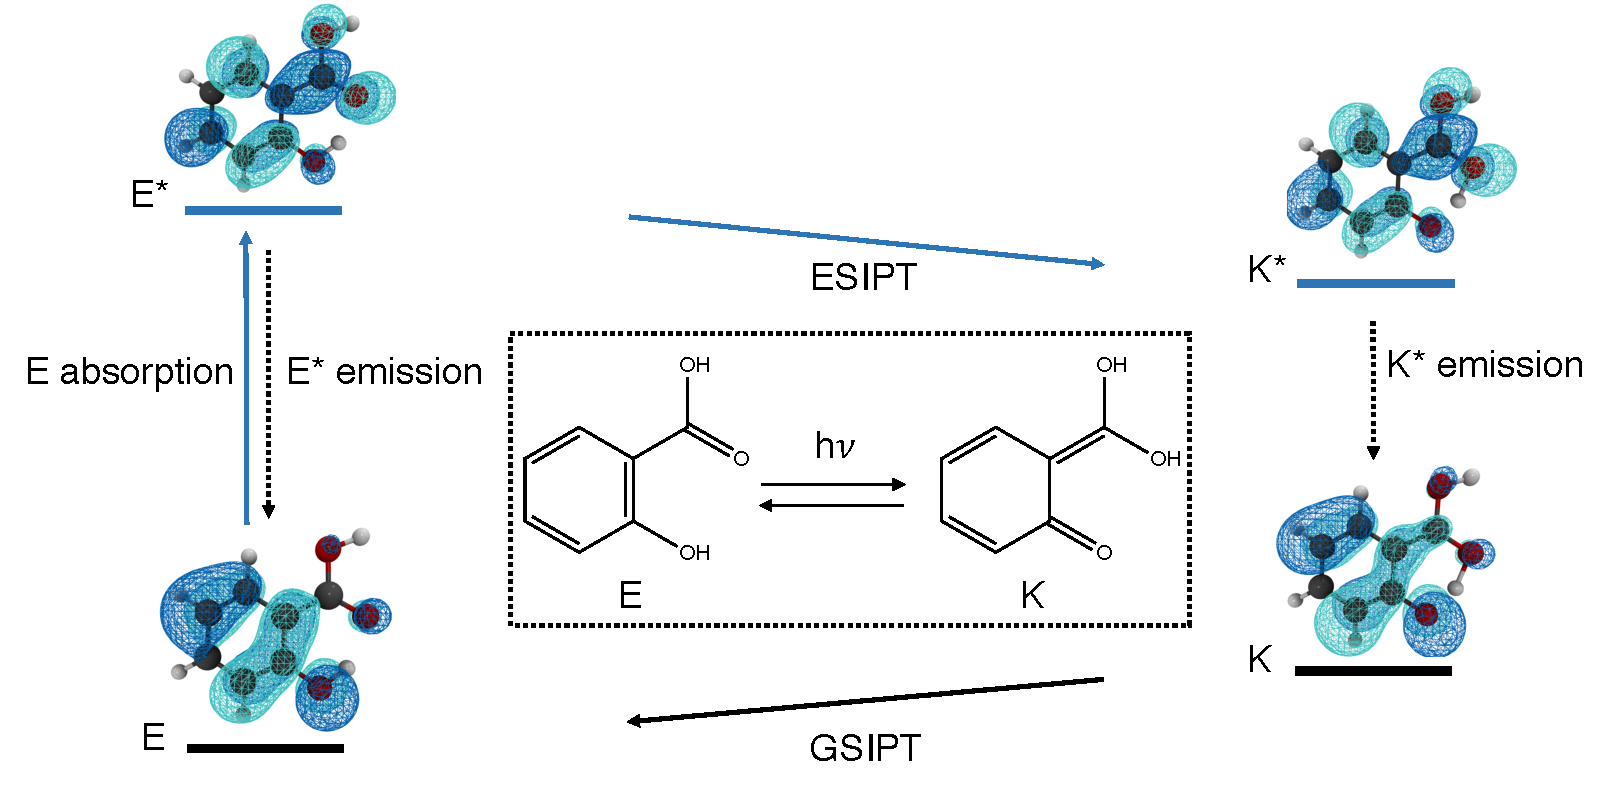
\includegraphics[width=0.95\linewidth]{1Intro/ESIPT.pdf}
  \caption[The four-level photocycle of \ac{ESIPT}]{The four-level photocycle of \ac{ESIPT} for salyclic acid. The HOMO and LUMO orbitals are also shown.}
  \label{figure: ESIPT}
\end{figure}
\subsection{The Four-Level Photocycle}
Inherent in all \ac{ESIPT} processes is a fully reversible four-level photocycle, the prerequisite for which is the presence of an intramolecular hydrogen bond. The proton donor can be an amino or hydroxyl group, while the proton acceptor is usually an imine or carbonyl. The four-level photocycle for salicylic acid is depicted in Figure \ref{figure: ESIPT}, along with the main molecular orbitals. The chromophore in the ground state (S\textsubscript{0}) is in the enol form (E), mediating hydrogen bond formation between the carbonyl oxygen and the hydroxyl proton. Upon electronic excitation, the excited state (\Estar, S\textsubscript{1}) the geometry remains unchanged but electronic redistribution acidifies the hydroxyl and increases the basicity of the carbonyl group, as a result of the population of the $\pi^\ast$ orbital on the carbonyl oxygen. In the excited state, the keto form (\Kstar) is more stable due to the redistributed electron density, and the proton migrates from the hydroxyl oxygen to the carbonyl oxygen. Depending on the system, fluorescence can occur from both the excited enol form (\Estar) and the excited keto form (\Kstar), although due to the ultrafast nature of the proton transfer the major emitting species is the keto tautomer.\cite{Zhao2012} 

For most \ac{ESIPT} processes containing strong hydrogen bonds, proton transfer is near barrierless and  occurs on a femtosecond time scale.\cite{Padalkar2015} The rate of the proton transfer and emission wavelength are highly sensitive to the surrounding medium and the presence of electron donor/acceptor moieties.\cite{Demchenko2013,Lin2017a,Li2017c} After fluorescence, the ground state keto form (K) is populated and the four level photocycle (E$\rightarrow$E$^{\ast}$$\rightarrow$K$^{\ast}$$\rightarrow$K) is completed. The initial geometry is restored through \ac{GSIPT}, although other photoproducts can be formed, for instance through cis-trans isomerisation or intersystem crossing.\cite{Al-Soufi1990}

\ac{AIE} in \ac{ESIPT} chromophores can be more complex than in non-polar propeller systems. The presence of hydrogen bonding sites enables the formation of intermolecular hydrogen bonds with solvent molecules, weakening the intramolecular bond and hindering \ac{ESIPT}.\cite{Cheng2015f} Kasha showed that the ratio of fluorescence intensity between \Estar and \Kstar dramatically changes based upon the solvent polarity.\cite{Kasha1986} In 3-hydroxyflavanone, the \Kstar fluorescence band is suppressed and the \Estar band increases in intensity with polar solvents. In strongly basic solvents, intermolecular proton transfer can occur between the chromophore and solvent, blocking access to the \Kstar state\cite{Laurent2014}. As touched upon earlier, the presence of donor acceptor groups opens the possibility of deactivation through \acf{TICT}. In solvent, the \ac{TICT} state is populated after proton transfer and lead to nonradiative decay. In a similar vain to \ac{RIR}, aggregation frustrates the torsional mode, preventing the \ac{TICT} from forming, and opens the radiative decay channel.\cite{Park2017,Wu2015a}
\subsection{Exploiting ESIPT and AIE for Applications}
The most investigated class of \ac{ESIPT} molecules are based on benzothiazole dyes, particularly \ac{HBT}.\cite{Padalkar2015,Kwon2011} The groups of Li and Liu investigated the effect of solvent for a range of \ac{HBT} derivatives, finding that increasing polarity impedes the proton transfer reaction and diminishes fluorescence. This is compounded by highly polar, protic solvents, where the hydroxyl proton can dissociate to form the phenolic anion. The proton transfer is highly sensitive to the solvent polarity, which is highly useful for sensing and probing applications.\cite{Wang2009,Cheng2015f} A \ac{HBT} analogue has been developed for ratiometric probing for hydrogen peroxide in living cells, where the \ac{ESIPT}-active fluorophore is produced by oxidative hydrolysis.\cite{Tang2018a} \ac{HBT}-based systems are also applicable for pH sensing, ion detection, biothol probing, and intracellular imaging.\cite{Kachwal2018,Kachwal2018,Liu2018}

Substitution of electron donor and acceptor groups onto \ac{ESIPT} cores can alter the proton transfer rate and stability of the enol and keto conformers on the excited state potential energy surface. In an extensive theoretical study, Jacquemin and co-workers investigated how different substitution patterns affect the emission from enol and keto states for a range of benzothiazoles.\cite{Azarias2016} They found that dual emission from both E$^*$ and K$^*$ is only possible in a small energy window for the compounds tested, and that the K$^*$ minimum can be favoured more drastically by dependent on the heteroatom in the core. The strongest substituent effects are seen with electron donor groups, such as methoxy, which stabilise the E$^*$ state. The K$^*$ state can be favoured by electron withdrawing groups in particular positions. Crucially, the effects of combining substituent groups is complex and depend on the specific \ac{ESIPT} core and substituent combination. The easily purturbed electronic structure of these systems make design from first principles extremely challenging.

\ac{ESIPT} cores are excellent candidates for optoelectronic applications on account of minimised self-absorption. However, the environment sensitivity which makes them so suitable for probing can be harmful to device stability.\cite{Kwon2011} Through chemical modifications, the Park group have fabricated stable \ac{OLED} devices with a range of emission frequencies.\cite{Park2008,Park2009,Kim2011} Introduction of carbazole gave access to blue K$^*$ emission, while \ac{EQE} values of 14\% have been reached by incorporating triplet harvesting via thermally activated delayed fluorescence with \ac{ESIPT}.\cite{Park2008,Mamada2017} Emission from both E$^*$ and K$^*$ enables white-light emission in devices, a highly attractive property due to the rarity of single molecule fluorophores with wide emission bands.\cite{Tang2011,Yao2011,Zhang2016b,Serdiuk2017}

The population inversion afforded by the \Kstar form makes \ac{ESIPT} systems attractive for laser applications.\cite{Fang2014,Gierschner2016} Additionally the large Stokes shift limits reabsorption and increases the optical gain.\cite{Kwon2011} In the 1980s, the principle of using \ac{ESIPT} for lasing applications was established by Kasha and co-workers for 3-hydroxyflavone, where the ultrafast proton transfer and double-well excited state potential energy surface lead to efficient population inversion.\cite{Khan1983,Chou1984} Since then, the structural diversity of \ac{ESIPT} systems have produced lasers with emission in the green, orange, and cyan regions.\cite{Sakai2016,Chen2016,Park2012,Park2008} Recently, an imidazole-based system with amplified spontaneous emission properties was developed with deep blue emission.\cite{Park2017} The restriction of the \ac{TICT} state in the crystalline form results in quantum yield of fluorescence of 67\%, producing an intense and narrow blue band for emission. 
\subsection{Harnessing ESIPT for Near-IR Emission}
Developing efficient fluorophore emission at the extremes of the visible spectrum is notoriously difficult. Whilst much attention has been paid to the blue region, the red and \ac{NIR} region is also hugely challenging in the solid state. The first system to exhibit solid state lasing properties in the \ac{NIR} region was reported in 2015.\cite{Cheng2015} The compounds were based on \ac{HC} skeletons and displayed \ac{ESIPT}. Interestingly, solid state fluorescence is only witnessed in some analogues, with substituent position and crystal packing modes determining the quantum yield of fluorescence. The question of whether electronic effects or the crystal structure determined the fluorescence activity was not fully resolved. Fluorine-containing derivatives with laser properties were published soon after.\cite{Cheng2016} In the same year, the same group published another breakthrough in solid state lasing, with structures based on  \ac{HP}.\cite{Tang2016} These compounds are similar to the \acp{HC}, but contain only one aromatic ring. Solid state fluorescence in single-benzene emitters is a rarity due to low melting points, but these systems showed extremely high fluorescence activity, surpassing the parent \ac{HC} systems.

\begin{table}[H]
\centering
\caption[Molecular structures and their QEs in the solid state]{Molecular structures of the \textbf{HC} and \textbf{HP} systems and their QEs ($\Phi_{\mathrm{PL}}$) in the solid state.\cite{Cheng2015,Tang2016,Cheng2016} } 
  \label{table: chalcones}
  \begin{tabular}{llllllll}
  %\hline
  \multicolumn{4}{c}{
  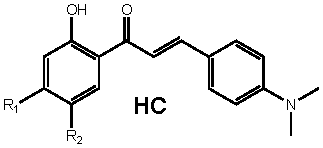
\includegraphics[height=2.7cm]{1Intro/HC.pdf}}
  & 
  \multicolumn{4}{c}{
  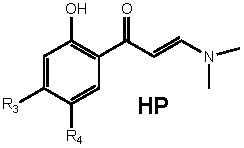
\includegraphics[height=2.7cm]{1Intro/HP.pdf}}\\
  \hline
  %\multicolumn{4}{c}{\textbf{HC}}&
  %&\multicolumn{4}{c}{\textbf{HP}}\\
  & R\textsubscript{1}
  & R\textsubscript{2}
  & $\Phi$
  &
  & R\textsubscript{3}
  & R\textsubscript{4}
  & $\Phi$\\
  \hline
  \textbf{HC1} & \ce{H} & \ce{H} & 0.32
  & \textbf{HP1} & \ce{H} & \ce{H} & 0.74\\
  %\hline
  \textbf{HC2} & \ce{CH3} & \ce{H} & 0.25
  & \textbf{HP2} & \ce{F} & \ce{H} & 0.84\\
   % \hline
  \textbf{HC3} & \ce{OCH3} & \ce{CH3} & 0.26
  & \textbf{HP3} & \ce{H} & \ce{OCH3} & 0.77\\
   %  \hline
  \textbf{HC4} & \ce{H} & \ce{CH3} & \textless0.01
  & \textbf{HP4} & \ce{H} & \ce{F} & 0.72\\
  %\hline
  \textbf{HC5} & \ce{H} & \ce{OCH3} &\textless0.01 & & & &\\
 % \hline
  \textbf{HC6} & \ce{F} & \ce{H} &0.41 & & & &\\
 % \hline
  \textbf{HC7} & \ce{H} & \ce{F} &0.10 & & & &\\
  \hline 
  \end{tabular}
\end{table}

For the \ac{HC} and \ac{HP} families, the crystal packing, absorption and emission wavelength, and crucially the QE, are all dependent on the choice of substituent and number of aromatic rings. How these factors interplay is not well understood. To fully understand the photophysical properties of these systems, intricate knowledge of the electronic, molecular picture must be combined with the intermolecular interactions inherent in the crystal as a whole. Theoretical methods can help elucidate this picture and offer insight into the working mechanisms behind \ac{AIE} for these \ac{ESIPT} systems, and how to maximise the quantum yield of fluorescence. This is the primary aim of the work in this thesis, with \ac{HC} and \ac{HP} families used as exemplars. In this thesis, Chapters \ref{chapter:NRdecay} and \ref{chapter: Inter} shall focus on the \textbf{HC} derivatives, with particular attention on \textbf{1} and \textbf{5}. In Chapter \ref{chapter: Connecting}, a holistic view of all eleven systems shall be taken as we examine how the crystal structure and packing regime influences emission. Since the \acp{HC} are the main focus of the thesis, the following section shall focus on their luminescent properties and previous investigations.  
%%%%%%%%%%%%%%%%%%%%%%%%%%%%%%
\section{Emitters based on 2'-hydroxychalcones}\label{section: lom HC}
%%%%%%%%%%%%%%%%%%%%%%%%%%%%%%
\subsection{Spectroscopic Investigations}
Research into \acp{HC}, and chalcones in general, has traditionally revolved around their metabolite character, since they are \textit{in vivo} precursors for a variety of flavones, flavonols, isoflavones, anthocyanidins, and other synthetic antioxidants.\cite{Singh2014} The \ac{ESIPT} process in \ac{HC} was first proven by Chou \textit{et. al.} in 1992.\cite{Chou1992} With an absorption band at 354 nm, and emission at 635 nm, the authors concluded that tautomerisation occurs upon absorption and that the keto S\textsubscript{1} state was responsible for emission. Cis-trans isomerism about the central double bond followed by molecular oxygen incorporation produces the flavanoid studied by Kasha, 3-hydroxyflavone. Previous studies had investigated this cyclisation mechanism, where it was initially thought cyclisation occurred through cis-trans isomerisation without proton transfer.\cite{Stermitz1975,Matsushima1985} It was later found that this isomerism could be hindered by solvent viscosity.\cite{Tokumura1998} Later, Arai and coworkers investigated the photochemistry of \textbf{HC} analogues, where they denoted the tautomerisation to be hydrogen atom transfer, rather than proton transfer.\cite{Arai1997,Norikane2002,Norikane2003,Kaneda2003,Kaneda2003a,Kaneda2004,Teshima2009} They mapped the potential energy surfaces using spectroscopic techniques to find that the cis-trans isomerism takes place in the triplet state, and only after hydrogen atom transfer. Most pertinent was their study of the effect of substituent on fluorescence in 2009.\cite{Teshima2009} Studying systems solvated in benzene, they discovered that the addition of a methoxy substituent \textit{meta} to the hydroxyl group in the phenol ring increased the quantum yield of red fluorescence by at least ten times, which the authors attribute to a combination of electronic and steric effects. The methoxy group stabilises the S\textsubscript{1} state through electron donation to the carbonyl \pipistar orbital whilst its size hinders the intramolecular modes. 
%%%%%%
\subsection{Crystalline Emission Properties}
%%%%%%
More recently, \textbf{HC} compounds have been developed for sensing and imaging applications. In 2014, the Tang group (of \ac{AIE} fame), developed a ratiometric fluorescent probe for sensing alkaline phosphatase based on 2'-hydroxychalcone.\cite{Song2014} Alkaline phosphotase is a dephosphorylating  enzyme, high concentration of which acts as a biomarker for diseases such as hepatitis, prostate cancer, and bone issues. By replacing the hydroxyl group of \textbf{HC} with a phosphoric acid group, the emission is yellow in aqueous conditions. In the presence of alkalane phosphotase, the cleave of phosphate and yields 2'-hydroxychalcone, which undergoes \ac{ESIPT} and emits in the red region. Another probe was developed to detect cysteine, again through the activation of \ac{ESIPT}.\cite{Li2017a} The \ac{AIE}/\ac{ESIPT} principle was applied using \textbf{HC} to develop a technique to detect latent fingerprints, for example in crime scenes.\cite{Jin2015} A fingerprint contains a high level of sebum, and when this is rinsed a \textbf{HC} solution, the \textbf{HC} molecules preferentially adhere to the fatty acid residues in the fingerprint, where they aggregate. When light is shone on the fingerprint, \ac{ESIPT} occurs and red fluoresence is produced, lighting up the fingerprint region against the dark backdrop of the substrate. 

In 2015, Zhang et al. synthesised a range of crystalline \textbf{HC} systems with different substitution patterns.\cite{Cheng2015} They found the identity and the position of the substituent to be critical in the quantum yield of the crystals. This is summarised in Figure \ref{figure: HC_experimental}. When substituents are \textit{meta} to  the hydroxyl group (compounds \textbf{1}-\textbf{3}) in the phenol ring, deep red fluorescence is observed, but only when in crystalline form. The solutions are almost non-emissive. Interestingly, under frozen conditions the solutions still only weakly fluoresce, indicating that restriction of intramolecular rotation is not the key factor in the \ac{AIE} for these molecules. When the same substituents are in \textit{para} position (compounds \textbf{4},\textbf{5}), neither the crystals nor the solutions are emissive. 
\begin{figure}[H]
\centering
  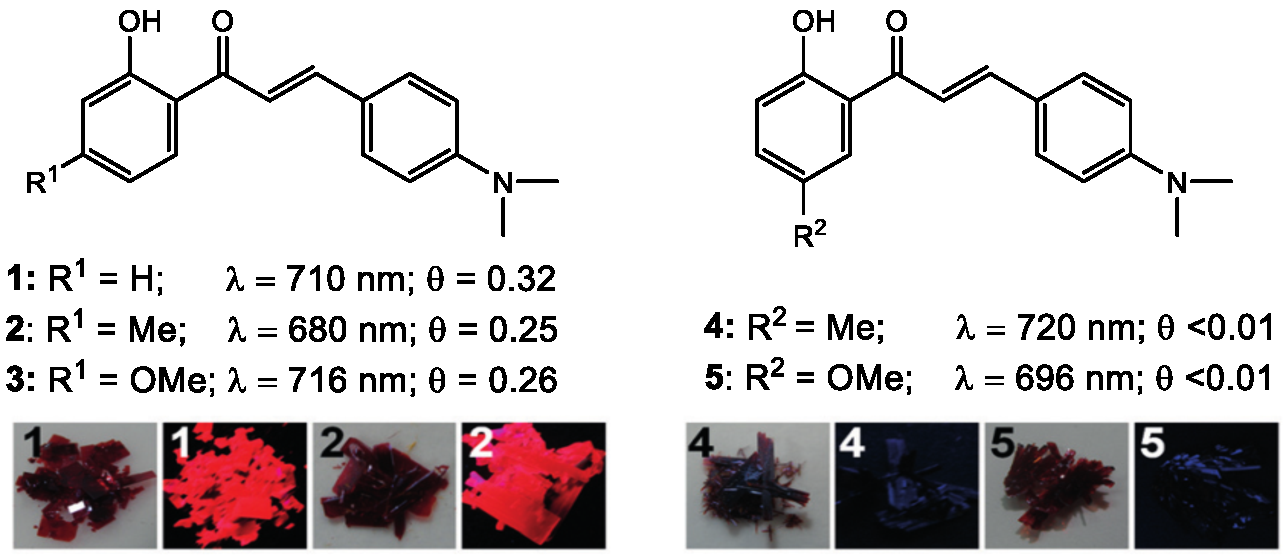
\includegraphics[width=0.95\linewidth]{1Intro/HC_experimental.pdf}
  \caption[Emission behaviour of crystalline 2'-hydroxychalcone derivatives]{Compounds \textbf{1}-\textbf{5} synethised by Zhang and coworkers. \textbf{1}-\textbf{} show high quantum yield, but \textbf{4}\&\textbf{5} are almost non-emissive. Absorbance maxima ($\lambda$) and quantum yields of fluorescence ($\theta$) are given, along with pictures of the dark and bright crystals for \textbf{1},\textbf{2},\textbf{4}, and \textbf{5}. Figure adapted from ref.~\citenum{Cheng2015} with permission of Wiley-VCH.}
  \label{figure: HC_experimental}
\end{figure}
These puzzling characteristics are attributed to both the planarity of the individual molecules and the packing in the crystal, as shown in Figure \ref{figure: HC_stacking}   Molecules \textbf{1}-\textbf{3} are almost completely planar and the strong intramolecular H-bonds, of length 1.753-1.780 \si{\angstrom}, increase the rigidity and planarity of the system. In the crystal, the molecules adopt an edge-to-face, herringbone packing mode preventing intermolecular $\pi$-interactions between the aromatic rings and enabling fluorescence from the keto S\textsubscript{1} state. For compound \textbf{4}, where a methyl substituent is \textit{para} to the hydroxyl, a similar edge-to-face packing mode is present. However, the molecule has a larger dihedral angle than \textbf{1}-\textbf{3}, which the authors attribute as the reason for the weak fluorescence. For \textbf{5}, the molecule is planar but the packing is face-to-face with aromatic stacking interactions. In the discussion, it is asserted that \textbf{5} is therefore non-emissive in the solid state due to excimer formation and non-radiative decay. The authors also hypothesise that the edge-face packed crystal of compound \textbf{4} shows minimal fluorescence because the molecule is not planar, despite other edge-face packed molecules brightly fluorescing, while the planar molecule does not emit because it is packed face to face.
\begin{figure}[H]
\centering
  \includegraphics[width=0.95\linewidth]{1Intro/HC_stacking}
  \caption[Crystal structures of 2'-hydroxychalcone derivatives]{The conformation of monomers \textbf{1},\textbf{4}, and \textbf{5}, along with their crystal structure. Crystal structures obtained from CCDC database codes from ref.~\citenum{Cheng2015}.}
  \label{figure: HC_stacking}
\end{figure}
It is with these hypotheses that this thesis begins. The first fundamental question is why do none of the five compounds fluoresce in good solvent? Secondly, in the solid state, why do only compounds \textbf{1}-\textbf{3} exhibit \ac{AIE}? Is this a substituent effect, as a result of the position of the methyl and methoxy groups, or is it due to the molecular packing mode, or is it a combination of both? Quantum chemical methods can identify the nonradiative decay channels in both dispersed and aggregated states, and therefore can elucidate the discrete electronic and intermolecular factors. In answering these questions, we can build understanding of how structure-property relationships operate in the \ac{AIE}/\ac{ESIPT} space and provide strategies for further optimising the fluorescence quantum yield of such systems.
%%%%%%%%%%%%%%%%%%%%%%%%%%%%%%
\section{Structure of thesis}\label{section: lom outline}
%%%%%%%%%%%%%%%%%%%%%%%%%%%%%%




\chapter{Chemistry on a Computer}
\label{chapter:theory}
\section{Quantum Mechanics and Chemistry}\label{section: QM}
\subsection{Overview}\label{section: QM_overview}
The development of quantum mechanics in the early 20th century armed scientists with the tools to calculate the microscopic properties of matter. In chemistry, the postulates of quantum mechanics can be applied to calculate relative energies of molecules, molecular geometries, ratios of products of chemical reactions, transition states, spectra, and any other phenomenon of interest. However, whilst in principle any property can be calculated exactly by the \schro{} equation, the analytical solution is only obtainable for systems with one electron. For systems larger than this, and therefore anything of observable chemical relevance, the computational expense on even modern computer architecture is intractable. 

To overcome this, a number of approximations are used in the field of computational chemistry to solve the multielectron problem. In general, as the number of atoms one wants to model increases, qualitative nature of the result also increases. Computational chemistry methods can generally be split into the types of approximations made and the number of atoms the method wishes to treat. In biophysical process and the modelling of proteins on the scale of tens of thousands of atoms, quantum mechanics is ignored completely. Forcefields are used to calculate the energy corresponding to a set of atomic coordinates in what are known as the \ac{MM} class of methods. The interactions between atoms are defined by analytical potentials, such as for bond stretches, bends, and angles, and are parameterised for different types of molecules using more accurate methods. This procedure is time-consuming and makes the forcefield specific to the systems it was fitted to, but enables computationally facile access to molecular geometries and properties of large systems.

At the other end of the scale the electronic structure is included through wavefunction or \ac{DFT} techniques. For the applications involved in this thesis, involving photoinduced phenomena, the activity of the electrons is paramount, and as such it is these methods which are utilised herein. In the next sections, the importance of the \schro{} equation shall be established, which along with the Born-Oppenheimer approximation enables the calculation of electronic properties through the simplest wavefunction method, the \ac{HF} method. Methods to improve the \ac{HF} approximation are then introduced, followed by the paradigm shift offered by \ac{DFT}. The first two sections of this Chapter focus on methods to obtain ground state properties, whilst in Section \ref{section: Photo} excited state methods shall be discussed. 
%%%%%%%%%%%%%%
%%%%%%%%%%%%%%
\subsection{The \schro{} Equation}\label{section: QM_schrodinger}
%%%%%%%%%%%%%%
%%%%%%%%%%%%%%
The wavefunction $\Psi$ contains all the information about the quantum state of the system at a position and time. As Newton's second law ($\bm{\mathrm{F}}=m\bm{\mathrm{a}}$) gives a classical particle's position and moment at each time period, thus describing it's classical state, so the time-dependent \schro{} equation does for wavefunction, and has the general form
\begin{equation}\label{equation: td-schro}
    i\hbar{}\frac{\partial \Psi(\bm{R},\bm{r},t)}{\partial t}=\hat{H}\Psi(\bm{R},\bm{r},t)
\end{equation}
where $\hbar=\frac{h}{2\pi}$ and $\hat{H}$ is the Hamiltonian operator for electrons at $\bm{r}$ and nuclei at $\bm{R}$. Separating the spatial part from the temporal part yields the time-dependent version of the \schro{} equation, which using the bra-ket notation of Dirac is\cite{Schrodinger1926}
\begin{equation}\label{equation: ti-schro}
   \hat{H}\ket{\Psi}=E\ket{\Psi}.
\end{equation}
This is an eigenvalue equation, where the Hamiltonian operator acts on the wavefunction to give the energy $E$ of the system. For a system of $N$ electrons and $M$ nuclei, the Hamiltonian calculates the kinetic ($T$) and potential ($V$) energy contributions of the electrons and nuclie towards the total energy of the system,
\begin{equation}\label{equation: H-simple}
\hat{H}=\hat{T}_{e}+\hat{T}_{n}+\hat{V}_{n-e}+\hat{V}_{e-e}+\hat{V}_{n-n}
\end{equation}
\begin{equation}\label{equation: H}
   \hat{H}=\underbrace{-\sum_{i=1}^{N}\frac{1}{2}\nabla_{i}^2 - \sum_{A=1}^{M}\frac{1}{2M_{A}}\nabla_{A}^2}_\text{kinetic terms}-\underbrace{\sum_{i=1}^{N}\sum_{A=1}^{M}\frac{Z_{A}}{r_{iA}}+\sum_{i=1}^{N}\sum_{j>{i}}^{N}\frac{1}{r_{ij}}+\sum_{A=1}^{M}\sum_{B>{A}}^{M}\frac{Z_{A}Z_{B}}{R_{AB}}}_\text{electrostatic terms}
\end{equation}
where $i$ and $j$ are electrons and $A$ and $B$ are nuclei. The first two terms are the operators for the kinetic energy of the electrons and the nuclei, where the Laplacian operator $\nabla^{2}$ is the second derivative of position. The next three terms are the electrostatic operators, summing the Coulomb interactions in the system;  the attractive interaction between electrons and the nuclei (of charge $Z$); the repulsive interaction between electrons; and the repulsive interaction between nuclei. Atomic units are used throughout, such that the electronic charge and mass are neglected. The $R$ and $r$ terms in the electrostatic parts denote the distance between nuclei and electrons.
%To calculate the energy $E$ , however, an eigenfunction for Equation \ref{equation: ti-schro}is required, corresponding to a wavefunction describing the electronic state.\cite{aszabo82:qchem}

In the hydrogen atom, the $\hat{V}_{e-e}$ and $\hat{V}_{n-n}$ can be neglected since there is only one proton and one electron, and the exact solution for the energy can be calculated since the wavefunction can be constructed analytically. However, for larger systems with many electrons and nuclei, Equation \ref{equation: ti-schro} cannot be solved. As such, a number of approximations must be made. The most fundamental of these is Born-Oppenheimer approximation.
%%%%%%%%%%%%%%
%%%%%%%%%%%%%%
\subsection{The Born-Oppenheimer Approximation}\label{section: QM_bornoppenheimer}
%%%%%%%%%%%%%%
%%%%%%%%%%%%%%
Separation of variables is a key concept in quantum chemistry, where a complex problem is broken down into constituent parts. This method is used to simplify the solving of Equation \ref{equation: ti-schro} by separating the electronic terms from the nuclear terms, and is known as the Born-Oppenheimer Approximation\cite{Born1927}
\begin{equation}
    \Psi_{BO}(\bm{R},\bm{r})=\Theta_{\bm{R},\bm{r}}\Phi_{\bm{r}}.
\end{equation}
where $\Theta_{\bm{R},\bm{r}}$ is the nuclear wavefuction and $\Phi_{\bm{r}}$ is the electronic wavefunction. The separation of terms is rooted in the fact that the nuclei are vastly heavier than electrons, and so it can be approximated that the nuclei are static with respect to the electrons. Equation \ref{equation: ti-schro} is solved, then, in two steps. First, the electronic structure is solved with ``clamped" nuclei, resulting in an electronic energy which is a parametric function of the nuclear coordinates. By concentrating on just the electronic terms, the \textit{electronic} Hamiltonian $\hat{H}_{e}$ becomes
\begin{equation}\label{equation: Hel}
     \hat{H}_{e}=\underbrace{-\sum_{i=1}^{N}\frac{1}{2}\nabla_{i}^2}_\text{kinetic term}-\underbrace{\sum_{i=1}^{N}\sum_{A=1}^{M}\frac{Z_{A}}{r_{iA}}+\sum_{i=1}^{N}\sum_{j>{i}}^{N}\frac{1}{r_{ij}}}_\text{electrostatic terms}.
\end{equation}
and the electronic \schro{} equation is then
\begin{equation}\label{equation: ti-schro-el}
   \hat{H}_{e}\ket{\Phi}=E_{e}\ket{\Phi}
\end{equation}

The total wavefunction $\Psi$ can considering multiple electronic states can be constructed from the combination of the electronic functions for each state $I$ and the corresponding nuclear wavefunction $\Theta_{I}$ in what is known as the Born-Huang expansion\cite{Born1954}
\begin{equation}
    \Psi(\bm{R},\bm{r})=\sum_{I}\Theta_{I}\Phi_{I}.
\end{equation}

When the nuclei are stationary, their kinetic energy is zero and the complete Hamliltonian is just the electronic Hamiltonian. For vibrating molecules, Equation \ref{equation: ti-schro-el} is solved at the required nuclear configuration, for electronic state $I$, and the time-evolution of the nuclear wavefunctions is\cite{Worth2004}
\begin{equation}\label{equation: nucwavefunctions}
    i\hbar{}\frac{\partial{}\Theta_{I}}{\partial{}t}=[\hat{T_{n}}+E_{I}]\Theta_{I}\underbrace{-\sum_{I}\hat{\Lambda}_{JI}\Theta_{I}}_\text{Nonadiabtic couplings}
\end{equation} 
%%%%%%%%%%%%COMMENT
\begin{comment}
\begin{equation}
    \sum_{A}\frac{1}{2M_{A}}\sum_{J\neq{}I}\hat{\Lambda}_{JI}\Theta_{I}=[\hat{T_{n}}+E_{I}(\bm{R})-E]\Theta_{I}
\end{equation} 
\end{comment}
%%%%%%%%%%%%COMMENT
where the energy of $E_{I}$ is the expectation value of the electronic Hamiltonian ($\bra{\Phi_{I}}\hat{H_e}\ket{\Phi_{I}}$). The highlighted \textit{nonadiabtic coupling} operator $\hat{\Lambda}_{JI}$ couples electronic state $I$ with electronic state $J$. In the adiabatic Born-Oppenheimer approximation, this coupling is completely neglected and the time-evolution of the nuclei becomes\cite{Yonehara2012}
\begin{equation}\label{equation: BO}
    i\hbar{}\frac{\partial{}\Theta_{I}}{\partial{}t}=[\hat{T_{n}}+E_{I}]\Theta_{I}
\end{equation} 
The nuclear motion is thus determined by the electronic energy of uncoupled \textit{adiabatic} states, and the nuclei move on the \ac{PES} of state $I$. $\hat{\Lambda}_{JI}$ contains the \textit{nonadiabatic} couplings, which become important when electronic states converge in energy. This shall be discussed in Section \ref{section: photo_conicals}

The Born-Oppenheimer approximation helps divide the problem into electronic and nuclear parts. However, solving the electronic problem exactly for many electron systems is impossible. In the next section, the mathematical building blocks of electronic structure methods, basis sets, shall be briefly described, after which methods to solve the electronic problem are introduced, starting with the \acf{HF} method. The \ac{HF} method is the fundamental quantum chemical approach to solve the many electron problem.
%%%%%%%%%%%%%%
%%%%%%%%%%%%%%
\subsection{Basis Sets}\label{section: methods_basisets}
%%%%%%%%%%%%%%
%%%%%%%%%%%%%%
Molecular orbitals are constructed from the linear combination of atomic orbitals. These atomic orbitals are represented by mathematical functions called a basis set. A complete set these functions, without any other approximations, would lead to the computation of the exact wavefunction (or energy). However, since an infinite basis set is not possible, another source of error in the electronic structure arises from the truncation of the basis set and the number of functions used. Atom-centred basis sets typically consist of Gaussian functions, which hold many numerical advantages over other functional forms for the wavefunction. To adequately describe valence orbitals, more than one basis function is used in what is known as the split valence. Adding polarisation and diffuse functions aid the long range description of the atomic orbital.\cite{Cramer2002}

For solid state calculations involving periodic systems, it is computationally more efficient to switch from atomic centred orbitals to periodic functions. In the solid state community, planewave basis sets are used to sample the unit cell, where the wavefunction is described by one-electron periodic functions ($e^{ikr}$). The wavefunction is constructed by summing these planewaves up to an energy cut-off as a function of the frequency. Often the core electrons are approximated by pseudopotentials to lower the computational cost of computing high frequency planewaves.\cite{Young2001} 

In the work presented in this thesis, almost all calculations involve atom-centred basis sets. Periodic DFT using planewaves are used to optimise the unit cells of molecular crystals, from which clusters are extracted and energies calculated as described in Section \ref{section: excited_states_crystals}. 

%%%%%%%%%%%%%%
%%%%%%%%%%%%%%
\section{Quantum Chemical Methods}\label{section: methods}
\subsection{The Hartee-Fock Method}\label{section: methods_HF}
%%%%%%%%%%%%%%
%%%%%%%%%%%%%%
In the \ac{HF} method, a single electron in an $N$-electron system moves within the field produced by the nuclei and the other $N$-1 electrons.\cite{hartree_1928} The intractable $N$-electron wavefunction $\Phi$ is simplified to be a product of $N$, one-electron wavefunctions $\chi$,
\begin{equation}
\ket{\Phi}=\ket{\chi_{1}\chi_{2}...\chi_{i}..\chi_{N}}.
\end{equation}
where $\chi$ are spin orbitals of each electron in the system. The spin orbitals consist of a spatial functional and a spin function, an infinite number of which could provide an exact solution. However, in practical terms a basis set of atomic functions is supplied, as described in Section \ref{section: methods_basisets}.\cite{szabo1996}
 
 From the Pauli exclusion principle, no two electrons may share exactly the same four quantum numbers (i.e occupy the same spatial and spin orbital). Since electrons are fermions, the electronic wavefunction is \textit{antisymmetric}, meaning that a change in the orbital must result in the wavefunction changing sign. This is enforced using Slater Determinants.\cite{Slater1929} This is most easily seen for a two-electron system for electrons at positions $\bm{x}_{1}$ and $\bm{x}_{2}$, where orbital $\chi_{1}$ contains electron at $\bm{x}_1$ and orbital $\chi_{2}$ contains electron at $\bm{x}_2$, with a normalisation factor of $N^{-\frac{1}{2}}$
\begin{equation}
\begin{split}
\Phi(\bm{x}_{1},\bm{x}_{2})&=\frac{1}{\sqrt{2}}\{\chi_{1}(\bm{x}_{1})\chi_{2}(\bm{x}_{2})-\chi_{1}(\bm{x}_{2})\chi_{2}(\bm{x}_{1})\}\\
&=\frac{1}{\sqrt{2}}
\begin{vmatrix}
\chi_{1}(\bm{x}_{1})&\chi_{2}(\bm{x}_{1})\\
\chi_{1}(\bm{x}_{2})&\chi_{2}(\bm{x}_{2})
\end{vmatrix}
\end{split}
\end{equation}
where by taking the determinant, the antisymmetry is ensured since exchanging the electrons changes the sign of the determinant. In the determinant, the rows consist of the electrons while the columns contain the orbitals. In the \ac{HF} method, the wavefunction is approximated by a single Slater Determinant, and therefore \ac{HF} is known as a single-determinant, or single-reference, method.  As well as ensuring antisymmetry, the Slater determinant wavefunction also introduces exact exchange (or HF exchange), a quantum mechanical property for electrons of parallel spin.\cite{szabo1996}

The variational principle states that the true ground state wavefunction will always be less than or equal to a trial wavefunction, meaning that the guessed spin orbitals will never undershoot the true energy. As such, 
\ac{HF} is a purely iterative method where the energy is computed for a set of trial spin orbitals, the spin orbitals are altered, and the energy is guessed again. This is repeated until convergence. 

To calculate the ``best" set of orbitals, the interactions in the electronic Hamiltonian are split into one-electron and two electron terms. The one electron terms are collected by the core Hamiltonian operator $\hat{h}_{i}$, involving the kinetic energy of the electrons and the electron-nuclei interactions,
\begin{equation}
    \hat{h}_{i}=-\frac{1}{2}\nabla_{i}^{2}-\sum_{A=1}^{M}\frac{Z_{A}}{r_{iA}}.
\end{equation}
The antisymmetric nature of the Slater determinent results in two operators for the electron-electron interaction, a Coulomb operator $\hat{J}_{ij}$ and an exchange operator $K_{ij}$, which act on orbital $\chi_{i}$ to determine the effect of the remaining orbitals,
\begin{equation}
    \hat{J}_{ij}\chi_{i}=\chi_{i}\int{\frac{\chi^{\ast}_{j}\chi_{j}}{r_{ij}}d\bm{x}_{2}}
\end{equation}
\begin{equation}
    \hat{K}_{ij}\chi_{i}=\chi_{j}\int{\frac{\chi^{\ast}_{j}\chi_{i}}{r_{ij}}d\bm{x}_{2}}.
\end{equation}
The Coulomb operator determines the Coulomb potential felt by electron $i$ in orbital $\chi_{i}$ from electron $j$ in orbital $\chi_{j}$. This is done by \textit{averaging} the interaction over all of the spatial coordinates of electron $j$. As such, $J_{ij}$ represents the average, or \textit{mean-field}, local potential felt by electron $i$. For this reason, the \ac{HF} method is often called a mean-field approach. The exchange operator $K_{ij}$ is a result of the antisymmetric Slater determinant, and is a quantum mechanical artefact of the fact that electrons are by nature  indistinguishable, and the exact labelling ($i$,$j$) has no physical meaning.\cite{szabo1996}

The one-electron and two-electron operators are collected by the Fock operator $\hat{F}$, such that
\begin{equation}
    \hat{F}=\hat{h}_{i}+\sum_{j\neq{}i}^{\frac{N}{2}}{[\hat{J_{ij}}-\hat{K_{ij}}]}
\end{equation}
The two electron terms run over only half of the electrons ($\frac{N}{2}$) to ensure interactions are not double counted, while the condition of $j\neq{}i$ means that an electron cannot interact with itself. 

The Fock operator allows Equation \ref{equation: ti-schro} to be solved in the \ac{HF} method through,
\begin{equation}\label{equation: Fock-operator}
    \hat{F}\ket{\Phi}=E\ket{\Phi}
\end{equation}
an eigenvalue equation solved by altering the orbitals until energy convergence is reached. In practice, for a closed shell system, the molecular orbital $\chi_{i}$ consists of a linear combination of $K$ atomic basis functions,
\begin{equation}\label{equation: expansion}
    \chi_{i}=\sum_{\mu=1}^{K}C_{ui}\phi_{\mu}\qquad\quad{}i=1,2,..,K
\end{equation}
The Roothaan-Hall equations are then used to solve Equation \ref{equation: Fock-operator} in matrix form,\cite{Roothaan1951,Hall1951}
\begin{equation}
    \bm{FC}={\bm{SC\epsilon}}
\end{equation}
where $\bm{F}$ is the Fock matrix containing the elements from the Fock operator, $\bm{C}$ contains the expansion coefficients from Equation \ref{equation: expansion} and $\bm{S}$ is the overlap matrix containing the overlaps of atomic orbitals ($\bra{\phi_{i}}\ket{\phi_{j}}$). By diagonalising the Fock matrix, $\epsilon$ is a diagonal matrix containing the orbital energies. \ac{HF} is commonly named the \ac{SCF} approximation, since the Roothaan equations are solved until self-consistency is reached.


The \ac{HF} method is a powerful approach to solving the electronic part of the \schro{} equation. However, it has several severe drawbacks which hinder its application and have resulted in more sophisticated methods being developed to address the shortcomings within. The most serious of these for ground state, closed-shell systems is the correlation problem. While electrons of parallel spin have the required exchange correlation, the Coulomb correlation is completely neglected since each electron sees only an average field of the other electrons. In reality, the motion of one electron is dependent on the motion of each of the other electrons, as depicted in Figure \ref{figure: mean-field}. This results in the energy of the system in \ac{HF} being overestimated in respect to the true energy. A number of methods to overcome the lack of correlation have been developed, which use the \ac{HF} method as a starting point before calculating the electron correlation. These are called post-Hartree-Fock methods, and those most relevant to the work in this thesis are discussed in the next section.
\begin{figure}[t]
\centering
  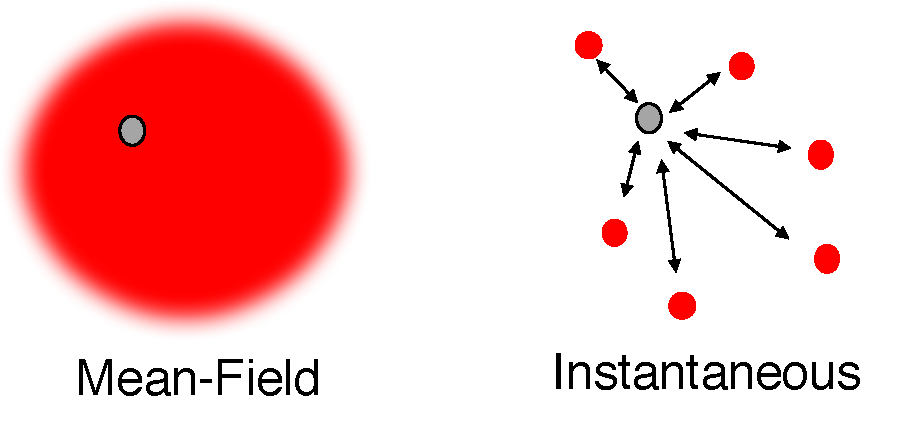
\includegraphics[width=0.4\linewidth]{2Theory/Mean_Field.pdf}
  \caption[Schematic of the mean-field approximation]{Depiction of the mean field electron interaction, where the electron of interest interacts with an average potential, rather than individually with each other electron.}
  \label{figure: mean-field}
\end{figure}

\subsection{Post-Hartre-Fock Methods}\label{section: methods_postHF}
%%%%%%%%%%%%%%
%%%%%%%%%%%%%%
\subsubsection{M{\o}ller-Plesset Perturbation Theory}
%%%%%%%%%%%%%%
Electron correlation energy can be added to the \ac{HF} energy by way of an external perturbative correction. In perturbation theory, the total Hamiltonian is divided into the zeroth-order part $\hat{H}_{0}$, which is the \ac{HF} Hamiltonian, and a perturbation $\hat{V}$, such that the eigenvalue equation becomes
\begin{equation}\label{equation: PT}
    \hat{H}\ket{\Phi_{i}}=(\hat{H}_{0}+\hat{V})\ket{\Phi_{i}}=\epsilon_{i}\ket{\Phi_{i}}.
\end{equation}
The eigenvalues and eigenfunctions of $\hat{H}_{0}$ are varied so that they become closer to the total Hamiltonian $\hat{H}$, which would then contain electronic correlation. This is done by the ordering factor $\lambda$, such that
\begin{equation}
    \hat{H}=\hat{H}_{0}+\lambda\hat{V}
\end{equation}
The true eigenvalues and eigenfunctions are expanded in a Taylor series in $\lambda$ up to $n$th order,
\begin{equation}\label{equation: MP2_energies}
    \epsilon_{i}=E_{i}^{(0)}+\lambda{}E_{i}^{(1)}+\lambda^{2}E_{i}^{(2)}+\lambda^{3}E_{i}^{(3)}+..+\lambda^{n}E_{i}^{(n)}
\end{equation}
\begin{equation}\label{equation: MP2_functions}
    \ket{\Phi_{i}}=\ket{\Phi_{i}^{(0)}}+\lambda{}\ket{\Phi_{i}^{(1)}}+\lambda^{2}\ket{\Phi_{i}^{(2)}}+\lambda^{3}\ket{\Phi_{i}^{(3)}}+..+\lambda^{n}\ket{\Phi_{i}^{(n)}}
\end{equation}
After inserting Equations \ref{equation: MP2_energies} and \ref{equation: MP2_functions} into Equation \ref{equation: PT} and collecting terms by order, the general expression for the total energy is
\begin{equation}
E_{i}=E_{i}^{(0)}+\sum_{n=1}^{n}\bra{\Phi_{i}^{(0)}}\hat{V}\ket{\Phi_{i}^{(n-1)}}
\end{equation}
The perturbation operator $\hat{V}$ introduces the Coulomb repulsion between electrons, which when combined with excited Slater determinants, recovers the \textit{dynamic} correlation energy. In most chemical applications, the method is contracted at second-order, and was initially employed by C. M{\o}ller and M.S. Plesset to obtain the correlation energy, hence the acronym \ac{MP2} is often used.\cite{Moller1934} Since MP is perturbative, the MP-calculated energy can be lower than the true energy, making it a non-variational method.
%%%%%%%%%%%%%%
\subsubsection{Coupled Cluster Theories}
%%%%%%%%%%%%%%
In an alternative approach to perturbation theory, \ac{CC} methods were introduced in the 1960s to account for electron correlation.\cite{Cizek1966,Paldus1972} \ac{CC} theory uses excited determinants by means of a Taylor expansion with an exponential operator
\begin{equation}\label{equation: cc}
    \ket{\Phi_{CC}}=e^{\hat{T}}\ket{\Phi_{0}}
\end{equation}
where $\ket{\Phi_{0}}$ is the \ac{HF} wavefunction and $\hat{T}$ is the cluster operator. The cluster operator produces a sum of excitation operators up to the truncation level $n$
\begin{equation}\label{equation: T}
    \hat{T}=\hat{T}^{(1)}+\hat{T}^{(2)}+\hat{T}^{(3)}+...+\hat{T}^{(n)}
\end{equation}
where $n$ is the excitation number. $\hat{T}^{(1)}$ includes all single excitations and $\hat{T}^{(2)}$ includes all double excitations, \textit{etc}.
%%%%%%%%%%%%%
%%%%%%%%%%%%
%For the first order, the contribution of all single excited determinants is 
%\begin{equation}
%    \hat{T}^{(1)}\ket{\Phi_{0}}=\sum_{i}^{occ}\sum_{a}^{vir}t_{i}^{a}\phi_{i}^{a}
%\end{equation}
%where $\phi_{i}^{a}$ is the excitation of an electron from occupied orbital $\phi_{i}$ to virtual orbital $\phi_{a}$, and $t_{i}^{a}$ is the amplitude given to this excitation.
%%%%%%%%%%%%%
%%%%%%%%%%%%
Substituting \ref{equation: T} into \ref{equation: cc}, and truncating at $n=2$, yields the coupled cluster wavefunction
\begin{equation}\label{equation: CCwavefunctioncomplete}
\ket{\Phi_{CC}}=e^{\hat{T}}\ket{\Phi_{0}}=\big[1+\hat{T}^{(1)}+(\hat{T}^{(2)}+\frac{\hat{T}^{2(1)}}{2})\big]\Phi_{0}
\end{equation}
As for perturbation theory, \ac{CC} theory is usually referred to by the trunctation level, for example CCSD refers to coupled cluster with single and double excitations. CCSD scales at $N^{6}$, adding considerable expense to the \ac{HF} method, which scales at $N^{4}$ (where $N$ is the number of basis functions).

%%%%%%%%%%%%%%
\subsection{Multireference Methods}\label{section: methods_multiconf}
%%%%%%%%%%%%%%
The methods described so far use \ac{HF} as a starting point and are thus built on a single-reference wavefunction. For a closed-shell system of an even number of electrons, orbitals are all doubly occupied. However, in many chemical processes, the electronic structure will deviate from this description and the wavefunction will not be dominated by one single electronic configuration, for example in bond dissociation, excited state processes, or when metallic elements are introduced. To describe these scenarios, the ground state wavefunction must incorporate other relevant electronic configurations, where more than one Slater determinant is used in the ground state wavefunction. These are termed multireference or multiconfigurational methods, and the multireference wavefunction is expressed as
\begin{equation}
    \ket{\Psi}=\sum_{m}c_{m}\ket{m}
\end{equation}
where $\ket{m}$ is the configuration state function containing optimised molecular orbitals and $c_{m}$ is the expansion coefficient for the state. In multireference methods, the molecular orbitals are divided into subspaces, where the active space contains the orbitals from which the important configurations are taken. In the configuration interaction method, the active space contains all of the molecular orbitals, with all excitations between the orbitals are considered, and thus all possible configurations are used in the wavefunction. This recovers the exact wavefunction (with an infinite basis set), but is prohibitively expensive such is the vast number of possible determinants, although these can be truncated to include only single excited states. More common is to use an active space containing occupied and virtual orbitals selected for their relevance for the problem in hand, and to only include excitations from within the $m$ active orbitals for $n$  electrons. This is called the \ac{CAS} method, which when used in combination with \ac{HF} for the remaining core orbitals (outwith the active space), is denoted \ac{CASSCF}.\cite{Roos1980} Due to the factorial scaling with the number of active orbitals, further space decomposition methods have been introduced through \ac{RAS}, where only certain excitations are allowed. Furthermore, using a state-averaging procedure can optimize the configuration state-functions for multiple states, to describe regions of strong electronic mixing. With these methods, the key parameter is often the choice of the active space - which orbitals to include, how many of them, and how many corresponding electrons. This is not a black-box procedure and will vary depending on the system of interest, the phenomena being modelled, and the computational resources available.\cite{Lischka2018} Recently, algorithms for automatic active-space selection procedures have been proposed.\cite{Stein2016,Bao2018}

Electron correlation can be divided into dynamic and static contributions. By incorporating the multireference character of the wavefunction, \textit{static} correlation is recovered in solving the \schro{} equation. The dynamical part is added on top of a reference wavefunction in the form of excitations, typically through perturbation theory as discussed in \ref{section: methods_postHF}. As such, most of the total correlation can be recovered by combining a multireference wavefunction with perturbation theory. This can produce accurate ground and excited state properties for chemical systems, although with rather large computational expense.\cite{Ramos-Cordoba2017,Stein2016a} A favoured approach is to combine \ac{CAS}\ac{SCF} with a \ac{PT2} calculation (\ac{CAS}\ac{PT2}), providing an effective protocol to calculate excited states. 
\subsection{Density Functional Theory}\label{section: theory_dft}
%%%%%%%%%%%%%%
The methods introduced thus far access chemical properties through some approximation of the wavefunction. An alternative approach is to disregard the wavefunction altogether and instead use the electron density to calculate microscopic properties of matter. This replaces the 3$N$ (+spin) variable of wavefunction methods by just 3 (+spin) spatial variables, allowing significant speed-up in \ac{DFT}. In 1964, Pierre Hohenberg and Walter Kohn proved a unique 1:1 correspondence exists between the ground state energy and the ground state density, and that all ground properties of a given $N$-electron system can be calculated from the ground state electron density ($\rho$).\cite{Kohn1964} The energy is thus a \textit{functional} (function of a function) of the electron density produced by a wavefunction,
\begin{equation}
    E[\rho]=\bra{\Psi[\rho]}\hat{T}+\hat{V}\ket{\Psi[\rho]}
\end{equation}
and, like \ac{HF}, obeys the variational principle.

\ac{DFT} is a mathematically exact formulation. However, the exact form of the functional relating the density to the energy is unknown. In 1965, Kohn and Sham developed a self-consistent approach to attain an approximation of the energy functional in equations that are ``analogous to the conventional Hartree and Hartree-Fock equations, and, although they also include correlation effects, they are no more difficult to solve."\cite{Kohn1965} In the Kohn-Sham system, a non-interacting system mimics the real interacting electron density. As in \ac{HF} where one-electron wavefunctions construct the N-electron wavefunction, so do single particle orbitals (Kohn-Sham orbitals $\phi$) construct the electron density,
\begin{equation}
    \rho=\sum_{j=1}^{N}|\psi_{j}|^{2}.
\end{equation}
The Kohn-Sham expression for the energy functional is written in terms of the kinetic and electrostatic interactions,
\begin{equation}
    E[\rho]=T_{e}[\rho]+E_{n-e}[\rho]+E_{e-e}[\rho].
\end{equation}
The most straightforward term to evaluate is the nuclear-electron interaction, which can be expressed as an electrostatic potential $V_{n}$ from the nuclei acting on the electronic density, 
\begin{equation}
    V_{n-e}[\rho]=\int{V_{n}(\bm{r})\rho(\bm{r})\mathrm{d}\bm{r}}.
\end{equation}
The electron-electron interaction can be separated into a classical, Coulomb-type expression and the quantum mechanical \ac{XC} part
\begin{equation}
    E_{e-e}[\rho]=\frac{1}{2}\underbrace{\int{}\frac{1}{r_{e_{1}e_{2}}}\rho(\bm{r}_{e_{1}})\rho(\bm{r}_{e_{2}})\mathrm{d}\bm{r}_{e_{1}}\mathrm{d}\bm{r}_{e_{2}}}_\text{Classical}+\underbrace{\vphantom{ \left(\frac{a^{0.3}}{b}\right) }E_{e-e}^{XC}[\rho]}_\text{XC}
\end{equation}
The kinetic energy of the interacting system is replaced by the kinetic energy of the non-interacting system, with the correction incorporated in to the \ac{XC} functional. It is the \ac{XC} functional which contains the crux of the problem in \ac{DFT}, since the exact form is unknown. It must be approximated. Much of \ac{DFT} development is focused on developing more accurate functionals to better describe specific chemical problems.

The first approximation to the functional is the \ac{LDA}. The LDA was originally proposed by Kohn and Sham in 1965 and depends only on the density at the coordinate in question. LDA approximates the molecular \ac{XC} energy by the \ac{XC} energy of a uniform electron gas. The \ac{XC} energy at a point in the molecule is then compared to a homogeneous electron gas with that density, for which the exchange can be solved analytically and the correlation is approximated through, for example, Monte-Carlo simulation.\cite{Ullrich2012} LDA works surprisingly well in structure prediction, given that the UEG has a uniform density whereas in reality the density varies with position in molecular systems. To incorporate the change of electron density with position, the \ac{GGA} functions include the density gradient, offering improved total energies, energy barriers, and geometries. Of the \ac{GGA} functionals, the PBE functional has become one of the most used in quantum chemistry.\cite{Perdew1996}

Hybrid functionals improve upon the \ac{GGA}s by including a percentage of \ac{HF} exchange energy. The \ac{XC} energy is expressed as a combination of the \ac{DFT} derived \ac{XC} and the \ac{HF} exchange energy. The hybrid version of PBE, PBE0, incorporates exact exchange \textit{via}
\begin{equation}
    E_{XC}^{PBE0}=\alpha{}E_{X}^{HF}+(1-\alpha{})E_{X}^{PBE}+E_{C}^{PBE}.
\end{equation}


One of the key errors in Kohn-Sham \ac{DFT}, using the types of functionals introduced thus far, is the self-interaction error. In \ac{HF}, the electron-electron interaction of the Hamiltonian ensures that an electron will interact with all the other electrons in the system but itself. In \ac{DFT}, each electron interacts with the entire electron density and thus with itself. If 100\% exact exchange is used this error is exactly cancelled. However, since this is not present in \ac{LDA}s or \ac{GGA}s, the \ac{XC}-potential does not show the correct asymptotic behaviour, and is only partially remedied by the small percentage of \ac{HF} exchange in hybrids. At large interelectronic distances, the self-interaction results in incorrect long-range asymptotic behaviour, where the \ac{XC} potential falls off more rapidly than 1/$R$.

To remedy this, a class of functionals called \acp{RSH} has been developed. The exchange is split into short- and long-range parts, where the short-range exchange will typically be represented by a local or semi-local functional, while the long range exchange is treated by \ac{HF} exchange. The distance at which the behaviour changes is determined by the range-separation parameter. Therefore, the long-range behaviour can be corrected due to having exact exchange. Whilst hybrid functionals are the most widely used in present day computational chemistry, it is certainly not a ``one size fits all" situation, since different functionals are developed to meet certain requirements, with development being ``property-driven" as much as rooted in theory. In particular, for dealing with excited states in \ac{TDDFT}, hybrid functionals have known and systamic failings, which the \ac{RSH} functionals aim to address. This shall be discussed in the next section, where the theory and techniques for modelling excited states are introduced.
%%%%%%%%%%%%%%%%%%%%%%%%%
%%%%%%%%%%%%%%%%%%%%%%%%%
\section{Modelling Electronically Excited States}\label{section: Photo}
%%%%%%%%%%%%%%%%%%%%%%%%%
%%%%%%%%%%%%%%%%%%%%%%%%%
\subsection{Overview}\label{section: photo_overview}
Thus far the methods introduced generally address thermal chemical processes, i.e those which occur in the electronic ground state. Modelling electronically excited states is a considerably more complex task, in terms of both the number of possible reaction paths and the methods needed to describe them. Some of these are illustrated in Figure \ref{figure: Jablonski}. The \acf{PES}, briefly introduced in Section \ref{section: QM_bornoppenheimer}, is absolutely central in understanding excited-state processes. It is through probing the \ac{PES} that feasible pathways, and thus chemical mechanisms, are elucidated and physical observables are rationalised theoretically.

\begin{figure}[t]
\centering
  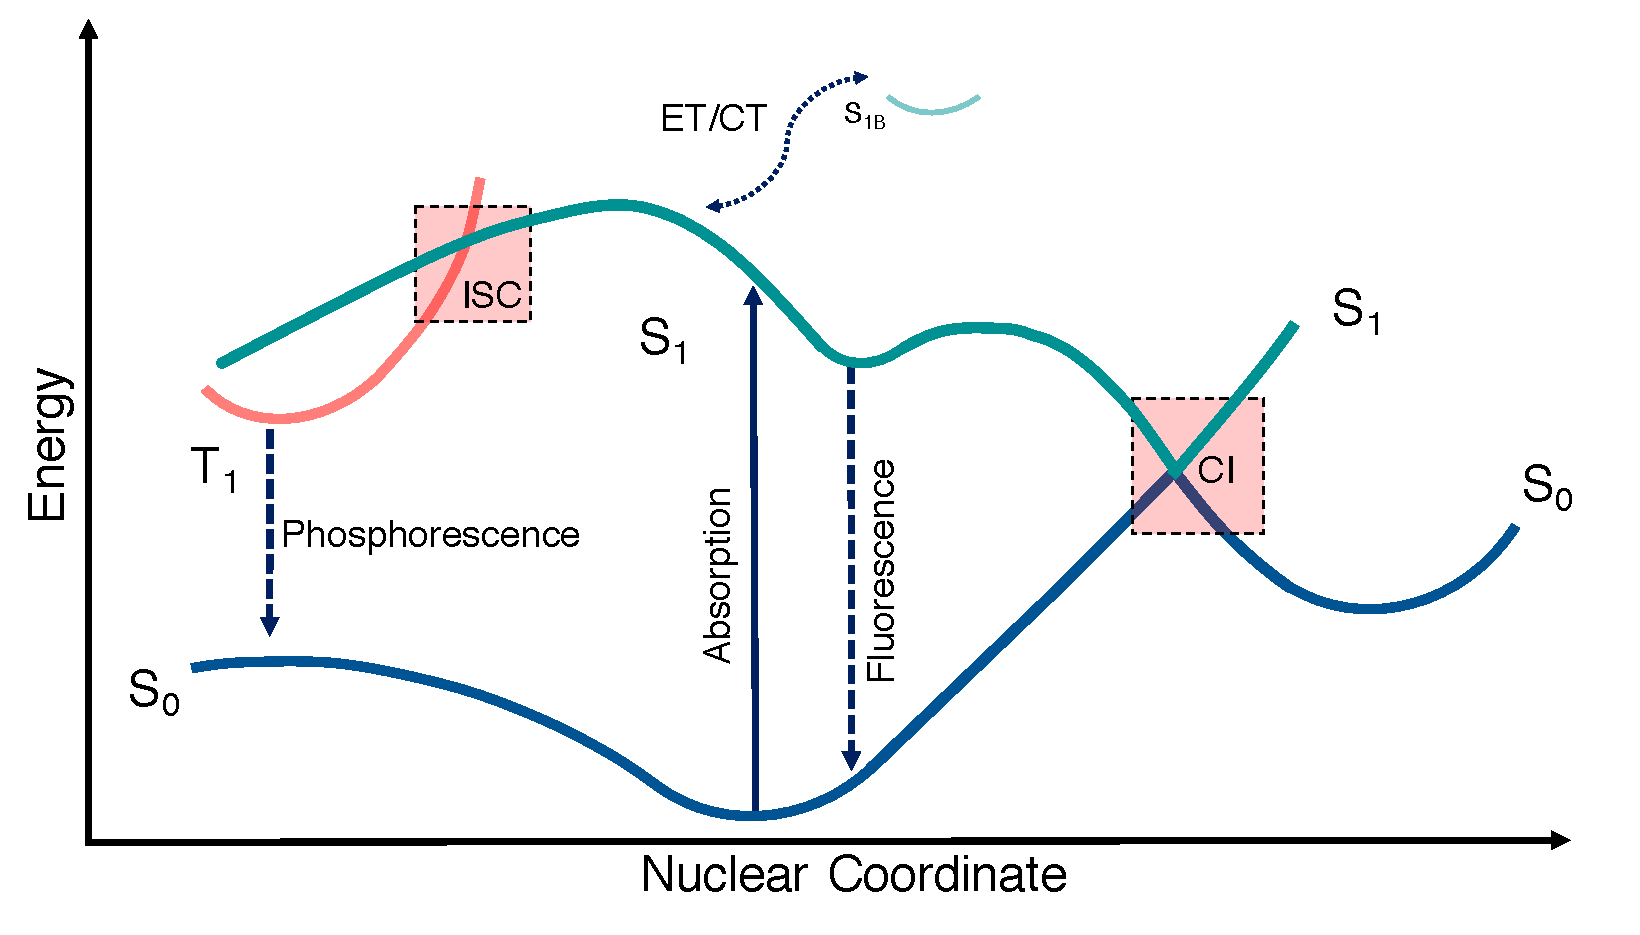
\includegraphics[width=0.8\linewidth]{2Theory/Jablonski.pdf}
  \caption[Relaxation pathways post electronic excitation.]{Competing relaxation pathways after electronic excitation to the first excited singlet state (S\textsubscript{1}. Nonradiative decay channels through conical intersections (CI), energy transfer (ET) and charge transfer (CT) to other molecules, compete with fluorescence. Alternatively, intersystem crossing (ISC) can occur, followed by phosphorescence.}
  \label{figure: Jablonski}
\end{figure}

Electronic excitation, induced by irradiation from the \ac{UV} or visible range, will normally occur at the thermal equilibrium geometry in the ground state. Absorption of a photon will place the system in an electronically excited state. According to the \ac{FC} Principle, the nuclei will undergo negligible change upon change in electronic state. This region of the \ac{PES} is called the \ac{FC} region, or point, and the electronic excitation is considered to be vertical (directly to the point of the upper \ac{PES} vertically above the ground state). From here, a multitude of relaxation processes are possible with vastly different timescales. The fastest process is typically relaxation to lowest vibrational state, occurring in femtoseconds, followed by fluorescence. At the other end of the scale, if there is significant spin-orbit coupling, crossing to a triplet state through \ac{ISC} followed by phosphorescence can take milliseconds. 

Calculating the relative energies of these relaxation pathways is a challenging task for a number of reasons. Firstly, whilst Figure \ref{figure: Jablonski} is a one-dimensional cut of a specific nuclear coordinate, the true \ac{PES} is a 3$N$-6 (3$N$-5 for a linear molecule) hypersurface of nuclear degrees of freedom. As such the full surface cannot feasibly be sampled for large molecules, and specific areas or modes are initally chosen. Secondly, the same ground state methods introduced in Section \ref{section: methods} must be tweaked or expanded upon to incorporate excited states. Thirdly, and perhaps most importantly, in certain regions of the \ac{PES} the fundamental principle of quantum chemical methods, the Born-Oppenheimer approximation, breaks down altogether. Such regions occur when two electronic states become close in energy, as highlighted in red in Figure \ref{figure: Jablonski}. In this region, the electronic states become directly coupled with the nuclear motion, breaking the Born-Oppenheimer approximation. These ``funnel" regions, or conical intersections, are crucial in modelling nonradiatve decay.

This section is organised as follows. Firstly, the importance of conical intersection will be discussed. Following, we will examine how excited-state mechanisms can be probed through nonadiabatic dynamics simulations. Finally, methods to perform these calculations, such as \acf{TDDFT}, shall be addressed. 
\subsection{Conical Intersections} \label{section: photo_conicals}
In photochemical processes with well-defined, well-separated electronic states, the adiabatic Born-Oppenheimer approximation is valid (Equation \ref{equation: BO}). That is, the nuclear wavefunction of an electronic state independent from the nuclear wavefunction of another state. However, as shown in Figure \ref{figure: Jablonski}, in photochemical processes there are regions on the energy landscape where electronic states become close in energy. In these regions, small changes in nuclear configuration results in large changes in the electronic wavefunction - hence the separation of nuclear and electronic wavefunctions is no longer valid and the Born-Oppenheimer approximation breaks down. In practice, this means that the nonadiabtic coupling terms become important and can no longer be neglected. The coupling operator $\hat{\Lambda}$ of Equation \ref{equation: nucwavefunctions} is defined as
\begin{equation}
    \hat{\Lambda}_{IJ}=\frac{1}{2M}(2\bm{F}_{JI}\cdot{}\nabla{}+G_{JI})
\end{equation}
where $\nabla$ the first derivative of position and
\begin{equation}
    \bm{F}_{JI}=\bra{\Phi_{I}}\nabla{}\ket{\Phi_{J}}
\end{equation}
is the derivative or nonadiabatic coupling vector with respect to position. $G_{JI}$ is the scalar coupling,
\begin{equation}
    G_{JI}=\bra{\Phi_{I}}\nabla{}^{2}\ket{\Phi_{J}}.
\end{equation}
$\bm{F}_{JI}$ is a 3$N$-vector coupling the nuclear motion of electronic state $I$ with state $J$. The total value is given by the scalar product of $\bm{F}$ with the nuclear momentum, and so the size (and thus the probability of a transition) is defined by the size of the coupling as well as the momentum of the nuclei.\cite{Worth2004}. The derivative coupling $\bm{F}_{JI}$ can be expressed in terms of the electronic Hamiltonian $H_{e}$, such that
\begin{equation}\label{equation: NAC_F}
        \bm{F}_{JI}=\frac{\bra{\Phi_{I}}\nabla{}\hat{H}_{e}\ket{\Phi_{J}}}{E_{J}-E_{I}}.
\end{equation}

With large electronic differences ($E_{J}-E_{I}$), the large mass difference between electrons and nuclei make $\bm{F}_{JI}$ inconsequentially small. However, as states converge the coupling increases. Only two coordinates can lift complete degeneracy, resulting in the \ac{PES} forming a double-cone structure. Conical intersections thus act as funnels, where the wavepacket can transfer nonradiatively between electronic states in an ultrafast timeframe. The two degrees of freedom define the branching space vectors. The first is the gradient difference vector $\bm{g}$, defining the difference between the gradients of the upper and lower \acp{PES},
\begin{equation}
    \bm{g}_{JI}=\bra{\Phi_{I}}\nabla{}\hat{H}_{e}\ket{\Phi_{I}}-\bra{\Phi_{J}}\nabla{}\hat{H}_{e}\ket{\Phi_{J}}.
\end{equation}
The second is the nonadiabatic coupling vector $\bm{h}$, defining the direction of strongest coupling between states, which is the numerator of Equation \ref{equation: NAC_F},
\begin{equation}
    \bm{h}_{JI}=\bra{\Phi_{I}}\nabla{}\hat{H}_{e}\ket{\Phi_{J}}.
\end{equation}
The vectors $\bm{g}$ and $\bm{h}$ are orthogonal, defining the plane of the conical intersection. $\bm{g}$ points in the direction of removing the energetic splitting, whilst $\bm{h}$ points towards maximising the nonadiabatic coupling. This is depicted in Figure \ref{figure: Cone}. Important to note is that for polyatomic molecules the conical intersection is not an isolated point but multidimensional. Displacement through any of remaining 3$N$-8 coordinates will retain the degeneracy, with the system moving on a degeneracy seam between the two surfaces.
\begin{figure}[H]
\centering
  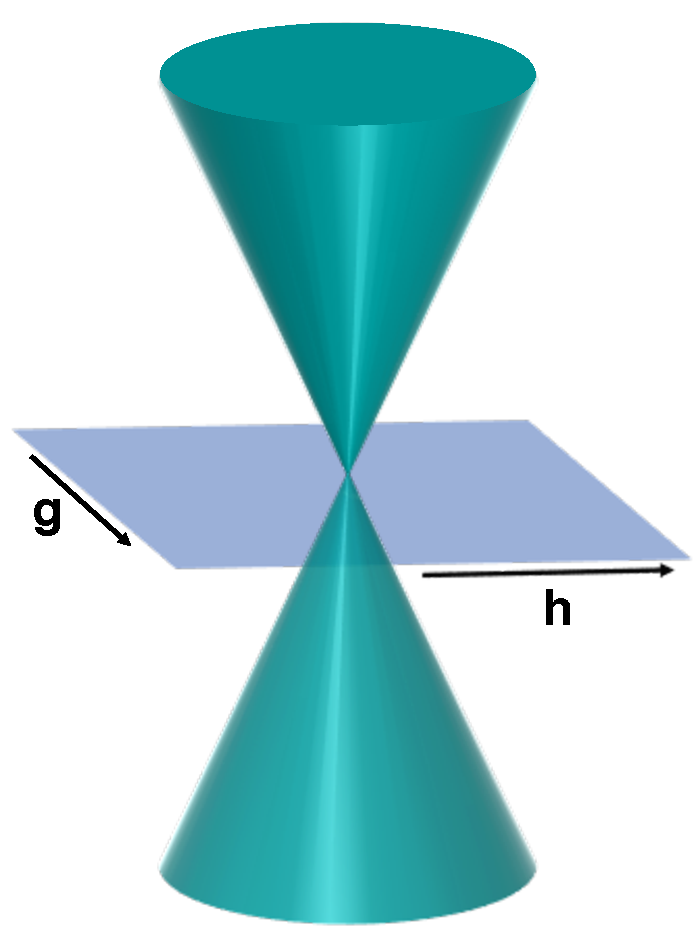
\includegraphics[width=0.4\linewidth]{2Theory/cone.pdf}
  \caption[Schematic of the double-cone topology of degenerate electronic states]{Schematic of the double-cone topology of degenerate electronic states. The gradient difference vector $\bm{g}$ and the nonadiabatic coupling vector $\bm{h}$ define the branching space lifting the degeneracy.}
  \label{figure: Cone}
\end{figure}
Locating conical intersections is important in determining the feasibility of nonradiative decay mechanisms.\cite{Domcke2011} In particular, the \ac{MECI} between the ground and first excited state is a local minimum on the S\textsubscript{1}/S\textsubscript{0} intersection seam and represents the lower bound for feasible crossings. Various methods to locate the geometry of \acp{MECI} for molecular systems have been developed using the gradient difference and nonadiabatic couplings vectors.\cite{Koga1985,Manaa1993,Bearpark1994,Dallos2004,Yarkony2004} 

In the majority of this work, we use the CIOpt algoirthm of Levine, Coe, and Martinez to locate \acp{MECI} for single-reference methods, where the derivative coupling vectors are not required.\cite{Levine2008} In CIOpt, Legrange multipliers are used to find the minimum of the objective function
\begin{equation}\label{equation: CIOpt}
F_{JI}(\bm{R},\sigma{},\alpha{})=\bm{E}_{JI}(\bm{R})+\sigma{}G_{JI}(\Delta{}E_{JI}(\bm{R},\alpha))
\end{equation}
where 
\begin{equation}
    \bm{E}_{JI}(\bm{R})=\frac{E_{I}(\bm{R})+E_{J}(\bm{R})}{2}
\end{equation}
and
\begin{equation}
    \Delta{}E_{JI}(\bm{R})=E_{J}(\bm{R})-E_{I}(\bm{R})
\end{equation}
where $G_{JI}(\Delta{}E_{JI}(\bm{R},\alpha)$ is a penalty function. Equation \ref{equation: CIOpt} minimises the average energy of states $I$ and $J$ with the penalty function penalising any step which increases the energy gap.  $\sigma$ alters the penalty weight whilst $\alpha$ is a smoothing factor. The interfacing of CIOpt with a variety of electronic structure codes allows \acp{MECI} to be located for a variety of quantum chemical methods. 

The topology of conical intersections calculated by different quantum chemical methods has attracted debate in the community.\cite{Levine2006a,Gozem2014,Tuna2015,Lefrancois2017} It has been shown that CASSCF and MS-CASPT2 (but not CASPT2) wavefunctions show the correct double-cone topology and a ``true" conical intersection. However, surfaces obtained with \ac{TDDFT} instead have a linear crossing due to there being no nonadiabatic coupling vector.\cite{Gozem2014}. ADC(2) methods also show a linear intersection, whereas \ac{CC}2 surfaces have the correct conical characteristics but are not completely quantitative.\cite{Tuna2015}. Therefore multireference methods are certainly preferable for modelling S\textsubscript{1}/S\textsubscript{0} crossings. However, single-reference methods can provide a qualitative description of the crossings and can produce reliable geometries. Dynamics simulations with these methods have shown for multiple systems that ADC2 and CC2 can provide reasonable results.\cite{Gozem2014,Tuna2015} In the case of TDDFT, a careful selection of the functional is required.\cite{Crespo-Otero2014,Barbatti2015} With the computational cost of multireference methods and the sensitivity of their active space, in this work we use a combination of single- and multireference methods, where \acp{MECI} obtained with \ac{TDDFT}, \ac{ADC2}, and \ac{CC}2 methods are compared to those obtained with CASSCF.

\subsection{Dynamics Simulations of Excited State Processes}\label{section: photo_dynamics}
Simulation of the temporal evolution of photoinduced processes is a powerful method for probing excited state \acp{PES}. Treating both nuclear and electronic motion fully quantum mechanically, with the required nonadiabatic couplings, is unfeasibly expensive for real molecular systems. As with all quantum chemical approaches, approximations are made. To retain the quantum description of the nuclei, specific nuclear modes can be sampled to reduce the dimensionality of the configuration space and the associated computational cost. Alternatively, the nuclear motion can be treated classically and allowed to explore the configuration space determined by the electronic \acp{PES}. 

The second approach, \ac{NA-MQC}, shall be used in elements of this thesis with the \ac{TSH} method. The most prominent \ac{NA-MQC} methods are \ac{TSH}, mean-field Ehrenfest, and multiple spawning.\cite{Crespo-Otero2018} In Ehrenfest dynamics, a nuclear trajectory is calculated using a weighted-average of a predefined number of electronic states. In multiple spawning, a series of Gaussian functions describe the nuclear wavepacket propagating on electronic surfaces. In the vicinity of state crossings, more Gaussian functions are spawned to follow each electronic state. With \ac{TSH}, a set of independent trajectories approximate the wavepacket propagation, with electronic transitions determined stochastically, most commonly using Tully's fewest-switches alogrithm.\cite{Tully1990} \ac{TSH} is perhaps the mostly used algorithm for simulating \ac{NA-MQC} dynamics, where the Newtonian progpoation of the nuclei, on-the-fly quantum chemical calculations, and straightforward parallelisation have encouraged wide adoption.\cite{Barbatti2011}

In \ac{TSH}, the nuclei propagate classically on a single, adiabatic electronic surface, governed by 
\begin{equation}\label{equation: nuclei_prop}
    \frac{\mathrm{d}^{2}\bm{R}}{\mathrm{d}t^{2}}=\frac{\bm{F}}{M}
\end{equation}
where the force $\bm{F}$ is proportional to the electronic gradient of the current state $I$
\begin{equation}
    \bm{F}=-\nabla{}\bra{\Phi_{I}}\hat{H}_{e}\ket{\Phi_{I}}.
\end{equation}
The nuclear motion is integrated typically using the velocity Verlet algorithm.\cite{Swope1982} At each nuclear timestep, the evolution of the electrons is governed by the time-dependent \schro{} equation, where the wavefunction is approximated as a linear combination of $K$ electronic states $\psi$
\begin{equation}
    \Phi{}=\sum_{K}c_{K}\psi_{K},
\end{equation}
allowing the \schro{} equation to propagate through the coefficients $c$
\begin{equation}\label{equation: sc-schro}
    \frac{\mathrm{d}c_{I}}{\mathrm{d}t}=\sum_{K}-c_{K}\big(\frac{i}{\hbar}H_{IK}+\Lambda_{IK}\big)
\end{equation}
where $H$ collects the energies and $\Lambda$ the nonadiabatic couplings. The time-derivatives of the nonadiabatic couplings can be computed through wavefunction overlaps from previous time steps, using a finite differences procedure.\cite{Pittner2009,Ryabinkin2015}

In practice, the initial state (at $t=0$) is chosen based upon the oscillator strenghts for the nuclear configuration in question. During propagation, the current state can change, or 'hop', from $I$ to $J$ based upon a probability $P$ defined by
\begin{equation}\label{equation: hopping_prob}
    P_{I\rightarrow{}J}=\mathrm{max}\bigg[0,\frac{-2\Delta{}t}{|c_{I}|^{2}}\mathrm{Re}(\Lambda_{IJ}c_{J}c_{I}^{\ast}))\bigg]
\end{equation}
which gives a hopping probability number $P$. For the hop $I\rightarrow{}J$ to occur, a randomly sampled number $r_{t}([0,1])$ is used to evaluate
\begin{equation}\label{equation: hop_condition}
    \sum_{K=1}^{J-1}P_{I\rightarrow{}K}<r_{t}\leq{}\sum_{K=1}^{J}P_{I\rightarrow{}J}
\end{equation}
A further condition that the energy does not increase after a hopping is also enforced. The nuclear equations are typically integrated in steps of \si{0.5}{fs}, while the electronic structure calculated are performed at these timesteps with interpolation between them to account for the faster oscillations to reduce the computational expense. Generally, the algorithm for \ac{TSH} involves the following steps:
\begin{enumerate}
    \item Calculate electronic energies, gradients and nonadiabatic coupling terms for a specific nuclear configuration
    \item Integrate Equation \ref{equation: sc-schro}
    \item Evaluate the hopping probability from Equation \ref{equation: hopping_prob} and determine the current state from Equation \ref{equation: hop_condition}
    \item Propogate the nuclei to a new configuration by integrating Equation \ref{equation: nuclei_prop}
\end{enumerate}
These steps are repeated until the maximum time for the simulation is reached. An ensemble of trajectories is done, where the above alogrithm is carried out for many starting nuclear configurations to obtain the average wavepacket propagation. The most compuationally demanding step is the first, where the electronic properties are calculated at each time step. 

The number of trajectories in the ensemble is important for proper evaluation of the configuration space. However, even with an infinite ensemble, the quantum features of the nuclear motion are generally missed in \ac{TSH}. This is due to the decoherence problem, where forcing the propagation along a single surface artificially prevents the amplitudes following other gradients. By applying a dechorence correction in Step 2., the \ac{TSH} average population of the independent trajectories should mimic the quantum behaviour if enough trajectories are sampled.\cite{Granucci2007} Further corrections in \ac{TSH} must be made in order to preserve kinetic energies in case of frustrated hopping events, where Equation \ref{equation: hopping_prob} is fulfilled but the energy condition is not.

\subsection{Methods for Excited States}\label{section: photo_methods}
One of the most popular methods for probing excited states is \acf{TDDFT}, first proposed in 1984 by Runge and Gross, and then extended in 1995 by Casida, TDDFT is a popular approach for modelling the properties of electronically excited states[66]. The fundamental idea within TDDFT is that the dynamics of a system can be completely described by its time-dependent density. Runge and Gross proved that there is a unique, 1:1 correspondence between time-dependent densities and potentials.\cite{Runge1984}  From the 1:1 correspondence it follows that the time-dependent density is a unique functional of the external potential (and vice versa). The time-dependent Hamiltonian, and thus the wavefunction, are also functionals of the density, allowing the deduction that all physical observables are functionals of the time-dependent density.

The key quantity in determining the time-dependent density in \ac{TDDFT} is the time-dependent \acf{XC} energy. Just as in \ac{DFT}, \ac{TDDFT} requires a suitable approximation of the \ac{XC}-energy. \ac{TDDFT} uses the \ac{XC}-energy from \ac{DFT} and to construct the time-dependent density, in what is known as the adiabatic approximation. The adiabatic approximation assumes that at each moment in time the \ac{XC}-energy depends only on the instantaneous density. Excitations are calculated in \ac{TDDFT} using linear response theory, which probes the response of a system to a weak perturbation.

A well-known failing in \ac{TDDFT} is the poor description of \acf{CT} excitations, where there is minimal orbital between occupied and virtual orbitals involved in a transition. TDDFT is known to underestimate \ac{CT}-excitation energies with \ac{LDA}, \ac{GGA}, and hybrids, since self-interaction means virtual orbital energies are systematically too low in energy. The \ac{RSH} functionals have been shown to mitigate this error for \ac{CT} excitations, with tuned \ac{RSH} functionals showing equivalent performance wave function methods for the prediction of excitation energies.\cite{Stein2009a,Kuritz2011,Kronik2012a} Within the current work, the \ac{RSH} functional $\omega$B97X-D is used in density functional calculations to incorporate these benefits.\cite{Chai2008} 

In addition, approximate \ac{CC} methods are used to calculate excited state properties of molecules, namely the \ac{CC}2 method. The \ac{CC}2 method was formulated in 1995 to approximate CCSD but with $N^{5}$ scaling and provide accurate excitation energies.\cite{Christiansen1995} In \ac{CC}2, the single excitations of CCSD are retained but the double excitations are approximated, with comparable ground state accuracy of MP2.\cite{Hattig2005} Response functions of \ac{CC}2 provide excitation energies and transition moments, making it a popular method in probing excited-state properties of molecules.\cite{Sneskov2012}

As an alternative but closely related approach, propagator methods are also used to calculate excitation energies and transition moments. The polarizer propagator introduces the effect of an external field, for instance the absorption of a photon. In the \ac{ADC2}, the polarizer propagator acts on the \ac{MP2} ground state to give excitation energies at similar accuracy but reduced computational cost compared to \ac{CC}2.

\subsection{Modelling Excited States in Molecular Crystals} \label{section: excited_states_crystals}
The theoretical treatment of excitations in molecular crystals is a relatively underdeveloped field compared to modelling of excited states in solution or even band gaps in periodic solids. The localised nature of excited states in molecular crystals lends to a molecular orbital description, since the excited state resides on typically one or two molecular units.\cite{Sauer1989} The low population of excited molecules in the crystal has led to the current practice of modelling clusters of molecules extracted from the crystal structure. In this methodology, the cluster is partitioned into regions which are treated at different levels of theory in ``multilayer" models. At the centre of a cluster lies a chromophore molecules (or molecules), to be treated at an appropriate level using quantum mechanical methods. To reduce the computational expense, the contribution of the surrounding environmental molecules to the total energy is calculated a lower level of theory, either through a \acf{MM} description (denoted QM:MM) or an efficient quantum mechanical method such as \ac{HF} (QM:QM'). QM:QM' approaches combining multireference methods with DFT are a promising extension, although the they have not yet been widely used in describing excited state phenomena.\cite{Libisch2014,Cheng2017,Cheng2017a} It is typical to freeze the positions of the environmental atoms to retain the crystal packing arrangement, such that only the QM atoms are allowed to relax during an optimisation. It is therefore desirable to first optimise the unit cell using plane wave methods.\cite{Presti2016} 

A popular route to obtaining the total energy of the cluster is the ONIOM method.\cite{Byun1999,Frisch2003,Chung2015a} In the field of \ac{AIE}, the multilayer ONIOM QM:MM protocol has been applied in many studies to understand the fluorescent behaviour of solid state organic compounds.\cite{Li2011,Li2013,Sun2015a,Presti2016a,Wilbraham2016,Wang2016,Peng2016,Fan2016,Presti2017a,Li2017b,Lin2017,Li2017e,Fan2017,Hestand2017} In the ONIOM method, the whole cluster is called the ``real" system and the region to be treated at the highest level of theory is laballed as the ``model". The total energy ($E_{ONIOM}$) for the cluster is calculated through a subtractive scheme,
\begin{equation}\label{equation: ONIOM}
E_{ONIOM}=E_{QM,Model}+E_{MM,real}-E_{MM,model}
\end{equation}
where the total energy is the sum of the QM energy of the model system with the MM energy of the real system. Subtracting the energy of the model system at the MM level ensures that its contribution is not double counted.\cite{Chung2015a} The QM level energy is calculated through the chosen method, typically (TD)DFT or CASSCF/CASPT2. The MM-level energy is obtained, for the Amber forcefield, through

\begin{equation}
\begin{split}
    E_{MM}&=\sum_{bonds}K_{r}(r-r_{eq})^{2}+\sum_{angles}K_{\theta}(\theta-\theta_{eq})^{2}+\sum_{dihedrals}\frac{V_{n}}{2}[1+\mathrm{cos}(n\phi{}-\gamma{})]\\
    &+\sum_{i<j}\bigg[s_{ij}^{VdW}\big(\frac{A_{ij}}{r_{ij}^{12}}-\frac{B_{ij}}{r_{ij}^{6}}\big)+s^{q}_{ij}\frac{q_{i}q_{j}}{\epsilon{}r_{ij}}\bigg].
\end{split}
\end{equation}
The first three terms evaluate the bonded interactions through chemical bonds, angles and dihedrals. The final non-bonded interaction term describes the van der Waals and Coulomb interaction between each atom in the system, which are scaled by $s^{vdW}$ and $s^{q}$.
In mechanical embedding, the cross-region electrostatic interactions are treated at the MM level, and as such the electronic Hamiltonian is not polarised (or influenced) by the environmental molecules. In electrostatic embedding, atom-centred point charges from the MM region are incorporated into the QM Hamiltonian $\hat{H}_{V}^{model,QM}$ by modifying the original Hamiltonian $\hat{H}^{model,QM}$
\begin{equation}
    \hat{H}_{V}^{model,QM}=\hat{H}^{model,QM}-\sum_{i}\sum_{N}\frac{s_{N}q_{N}}{r_{iN}}+\sum_{J}\sum_{N}\frac{Z_{J}s_{N}q_{N}}{r_{JN}}
\end{equation}
where $N$,$J$, and $i$ refer to the MM atoms, QM atoms, and electrons respectively.\cite{Vreven2006} The scaling factor $s_{N}$ prevents overpolarisation of the wavefunction from atoms close to the QM region. The final term is also included in the MM evaluation of the model system, to ensure direct cancellation. The electrostatic embedding scheme provides a direct perturbation of the electronic structure by the environment. 

A potential deficiency arising from a standard ONIOM calculation for a cluster model is the neglect of the periodic nature of the molecular crystal. The truncation of the crystal into a cluster naturally removes the electrostatic long-range potential. To overcome this, other fields have research have applied the Ewald summation technique, which calculates the exact nature of the crystalline electrostatic potential.\cite{Weber2010,Stueber2001b} The Ewald method as implemented by Derenzo and coworkers does this through a five step algorithm:\cite{Klintenberg2000,Derenzo2000}  
\begin{enumerate}
    \item the point charges from a unit cell are assigned to the atoms of a supercell centered around a defect of interest called the quantum cluster.
    \item A chosen number of sample sites are randomly sampled in the quantum cluster region.
    \item A spherical region is then defined so that the quantum cluster and a number of additional points are included within a chosen radius. The points within that region will maintain their original charge values whereas the remaining points will be allowed to vary.
    \item An Ewald potential is calculated at each fixed value point (including points in the quantum cluster) and at the random sites from step 2.
    \item A system of linear equations is solved with respect to the variable charge values to match the direct sum of all charges in the system to the Ewald potentials calculated in step 4, whilst driving the overall charge and dipole moment to zero.
\end{enumerate}
The Ewald method was applied to excited states in molecular crystals in 2016 by Wilbraham \textit{et al.}\cite{Wilbraham2016} As the authors point out, the Ewald scheme is superior to traditional point charge embedding which inevitably involves some kind of charge truncation and the subsequent loss of periodicity. The Ewald method in contrast aims to reproduce the exact potential on the chromophore. For their case, an ESIPT/AIE system was chosen as a test molecule, such is the importance of the environment on the electronic structure. 
A second shortcoming of the ONIOM approach alone for excited states is the lack of polarisation of the MM region from the QM region. In the electrostatic embedding scheme, the QM region is polirased by the MM environment, but there is no mutual polarisation from the QM region \textit{back} to the MM atoms. Wilbraham and co-workers have attempted to remedy this through a self-consistent polarisation scheme, where the MM point charges and QM charges are altered until convergence.\cite{Wilbraham2016} This has been shown to be more effective than embedding alone for modelling absorption and emission in molecular crytals.\cite{Presti2017a,Wilbraham2018a} However, by treating the environment point charges and the chromophore charges at the same level of theory, the former necessarily correspond to a fully excited molecular crystal, which is perhaps nonphysical. This has been addressed by Miguel Rivera in our group, who has worked on the development of self-consistent embedding schemes to extend the method of Wilbraham. There are implemented in the \texttt{fromage} package. Due to the implementation timeline, self-consistent embedding schemes were not included in the work of this thesis. 

\chapter[Nonradiative Decay Mechanisms in 2'-hydroxychalcones]{Nonradiative Decay Mechanisms\\ in 2'-hydroxychalcones}
\label{chapter:NRdecay}
\begin{figure}[H]
\centering
  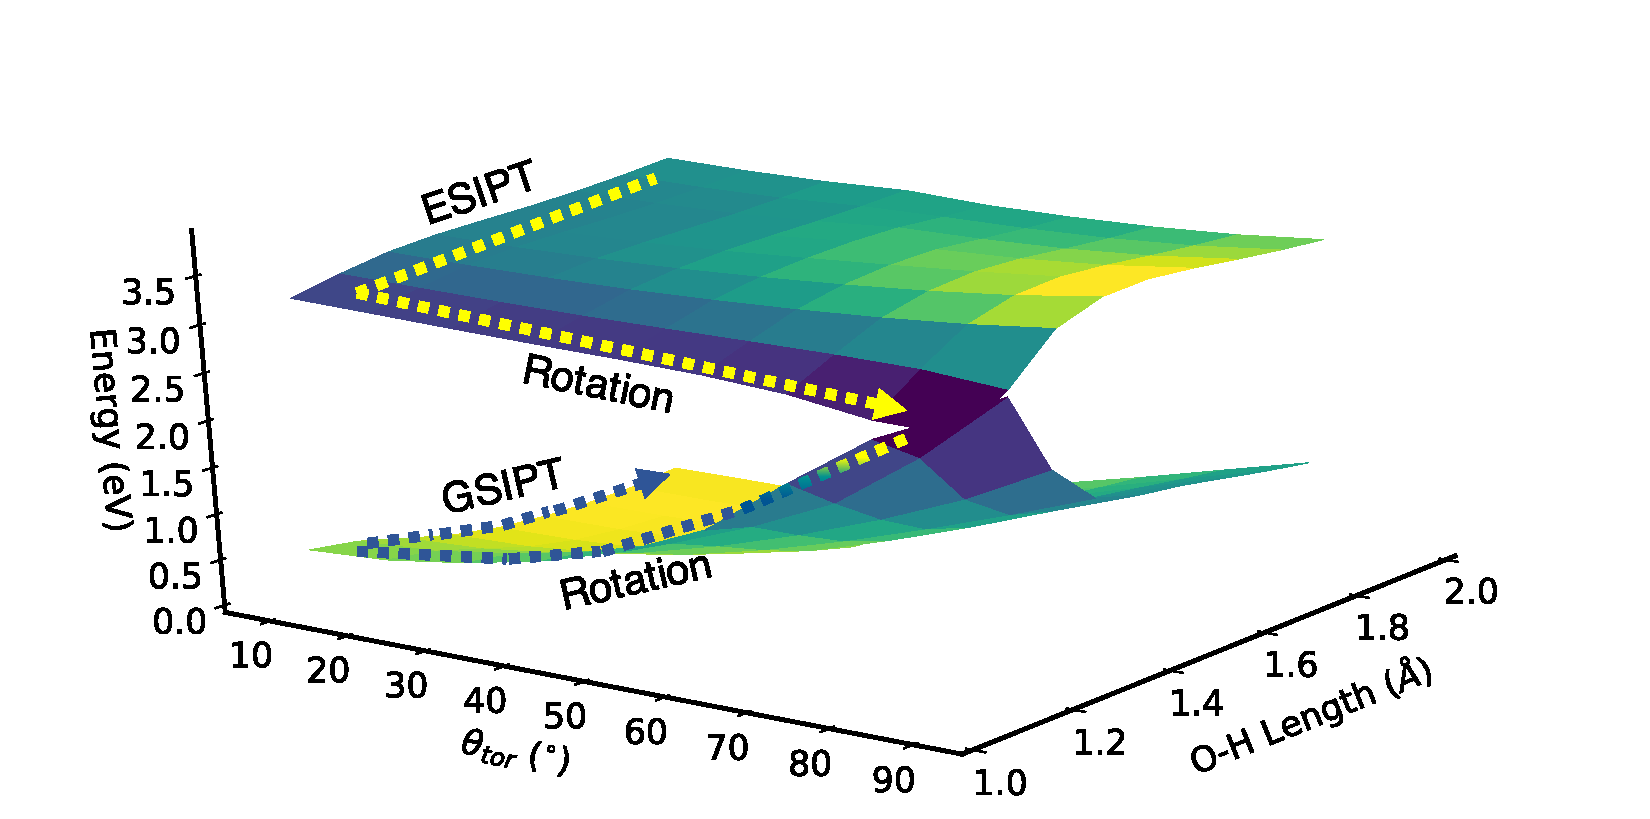
\includegraphics[width=0.7\linewidth]{3nonradiativedecay/1toc.pdf}
\end{figure}
\section{Introduction}\label{section: NRdecay_intro}
Computational methods have the potential to explain the intriguing luminescence properties of the \acf{HC} materials introduced in Section \ref{section: lom HC}. \textbf{HC} derivatives \textbf{1}-\textbf{5} of Figure \ref{figure: HC_experimental} have strikingly different emission characteristics in the solid state, for which we wish to disentangle the intra- and intermolecular contributions. This chapter addresses the intramolecular interactions present in the five systems. The effect of the substituents on the four level \ac{ESIPT} photocycle are analysed through a combination of static and nonadiabatic dynamics simulations, investigating the relaxation mechanisms and the competition between different deactivation channels in vacuum. These simulations show that a strong electron donating group (EDG) in the \textit{para} position alters the topology of the potential energy surface (PES), destabilising the \Estar{} state, thereby assisting and accelerating proton transfer. Our results provide detailed understanding into the fundamental relaxation mechanisms of \ac{HC}s and the role of the substituents, which is the initial step in unravelling the effect of aggregation on the emission properties.

This majority of the work presented in this chapter was published in reference\citenum{Dommett2017}. To complement the published work, herein there is additional analysis of the nonadiabatic dynamics simulations, where rate constants and lifetimes are explored in more detail. The computational methods used shall be described, followed by analysis of the vertical excitations, minima on the excited state, and the feasible relaxation channels. Finally the results of nonadiabatic dynamics rationalise those obtained in static calculations. The relevant Supporting Information of ref.\citenum{Dommett2017} is incorporated into the chapter and designated appendices.

\section{Computational Methods}\label{section: NRdecay_methods}
The ground state geometries of all the compounds were optimised in vacuum using resolution of identity \acf{MP2} with the def2-SV(P) and def2-TZVP basis sets.\cite{Haase1993,Schafer1992,Weigend2005} Vertical excitation energies were calculated in vacuum using coupled cluster to approximated second order (CC2) and \acf{ADC2} methods under the resolution of identity approximation with the def2-TZVP basis set.\cite{Christiansen1995,Hattig2000,Hattig2002,Kohn2003,Hattig2005} Core electrons were frozen for all \ac{MP2}, \ac{ADC2} and CC2 calculations. The performance of the ADC(2) and CC2 methods is compared, whilst the effect of the basis set is considered for ADC(2). 

Geometry optimisation in the first excited state was carried out in vacuum for \textbf{1}-\textbf{5} with ADC(2) and CC2 methods using the same basis sets as the ground state optimisation. These calculations were performed with Turbomole v7.0.\cite{Turbomole} The level of theory considered to discuss the features of the surfaces is CC2/def2-TZVP, unless otherwise specified.

The CIOpt software package of Levine, Coe, and Martinez was used to determine the location of the \acf{MECI} structures.\cite{Levine2008} The MECI structures were obtained for \textbf{1}-\textbf{5} at the CC2/def2-TZVP, ADC(2)/def2-TZVP, and ADC(2)/def2-SV(P) levels of theory. In the case of \textbf{1}, \ac{CASSCF} calculations were performed with MOLPRO program.\cite{Molpro} The \sone/\szero{} conical intersections were optimised with state-averaged CASSCF (SA-CASSCF). The active space considered 12 electrons in 11 orbitals (CASSCF(12,11)) including 2 states in the average with the 6-31G(d) basis set. The CASSCF(14,13) active space was also considered, shown in Appendix A. The \acp{PES} were explored through \ac{LIIC} pathways with ADC(2)/def2-TZVP level of theory. In the case of \textbf{1}, the intermediate \ac{LIIC} geometries were relaxed with the $\theta_{tor}$ angle fixed at the CC2/def2-TZVP level of theory. The geometries along the intersection seam were located using CIOpt. 

The absorption spectra of \textbf{1}-\textbf{5} were simulated using the nuclear ensemble method. 500 nuclear configurations were generated based on a Wigner distribution of the harmonic frequencies calculated at MP2/def2-SV(P) level of theory.\cite{Crespo-Otero2012} Five excited states at ADC(2)/def2-SV(P) level of theory were calculated for each individual geometry. For \textbf{1} and \textbf{5}, \acf{TSH} nonadiabatic dynamics simulations were performed using NEWTON-X interfaced with Turbomole, at ADC(2)/def2-SV(P) level of theory.\cite{Barbatti2014} The initial conditions for the dynamics were generated from the absorption spectra considering an energy window of $\pm$ \si{0.15} {eV} in the absorption spectra, simulating laser excitation.\cite{Barbatti2007} The geometries contributing to these energy windows were used as initial for the trajectory propagation along with their velocities and momenta. \szero{}, \sone{}, and \stwo{} states were included in the dynamics. 

For compound \textbf{1}, an energy window at absorption maximum of 3.35 $\pm$ 0.15 eV was selected for the nonadiabatic dynamics. 50 trajectories were statistically distributed between \sone{} (30) and \stwo{} (20), according to their oscillator strengths. The same protocol was used for compound \textbf{5}, with 50 trajectories (\sone: 30 and \stwo: 20) from an energy window of 3.39 $\pm$ 0.15 eV. The maximum simulation time was 500 fs, with a time step of 0.5 fs and the quantum equations were integrated with 0.025 fs using interpolated quantities between classical steps. Nonadiabatic effects were included using the fewest-switches surface hopping algorithm with decoherence corrections (0.1 Hartree). Nonadiabatic couplings between \stwo{} and \sone{} were estimated approximately using an approximated wave-function and the numerical method.\cite{Ryabinkin2015} The trajectories were terminated when the energy gap between \sone{} and \szero{} was less than 0.1 eV.

\section{Results}\label{section: NRdecay_Results}

\subsection{Vertical Excitations}\label{section: NRdecay_VE}
\begin{table}[t]
    \centering
    \begin{tabular}{cccccccccccc}
    \hline
     & \multicolumn{3}{c}{ADC(2)/def2-SV(P)} & & \multicolumn{3}{c}{ADC(2)/def2-TZVP} & & \multicolumn{3}{c}{CC2/def2-TZVP}\\
    \hline
     State & $\Delta$E & \textit{f} & Character & & $\Delta$E & \textit{f} & Character & & $\Delta$E & \textit{f} & Character\\
    \hline
    & \multicolumn{11}{c}{Compound \textbf{1}}\\
     \hline
      \sone   & 3.53 & 0.604 & \pipistar & & 3.36 & 0.869 & \pipistar & & 3.43 & 1.135 & \pipistar\\ 
      \stwo   & 3.58 & 0.391 & \npistar & & 3.44 & 0.090 & \npistar  & & 3.67 & 0.009 & \npistar \\
      \sthree & 3.97 & 0.013 & \pipistar  & & 3.77 & 0.008 & \pipistar & & 3.84 & 0.003 & \pipistar\\ 
      \hline
     & \multicolumn{11}{c}{Compound \textbf{2}}\\
     \hline
     \sone   & 3.53 & 0.483 & \pipistar  & & 3.38 & 0.806 & \pipistar & & 3.43 & 1.167 & \pipistar  \\ 
     \stwo   & 3.59 & 0.551 & \npistar  & & 3.46 & 0.196 & \npistar &  & 3.68 & 0.023 & \npistar \\
     \sthree & 3.96 & 0.010 & \pipistar  & & 3.77 & 0.007 & \pipistar &  & 3.85 & 0.005 & \pipistar \\ 
     \hline
     & \multicolumn{11}{c}{Compound \textbf{3}}\\
     \hline
     \sone   & 3.59 & 1.022 & \pipistar & & 3.40 & 1.063 & \pipistar  &  & 3.47 & 1.286 & \pipistar \\
     \stwo   & 3.64 & 0.075 & \npistar  & & 3.51 & 0.013 & \npistar   &  & 3.75 & 0.002 & \npistar \\
     \sthree & 4.06 & 0.046 & \pipistar & & 3.86 & 0.038 & \pipistar  &  & 3.96 & 0.034 & \pipistar \\ 
      \hline
     & \multicolumn{11}{c}{Compound \textbf{4}}\\
     \hline
     \sone   & 3.53 & 0.404 & \pipistar & & 3.36 & 0.857 & \pipistar &  & 3.42 & 1.105 & \pipistar  \\
     \stwo   & 3.57 & 0.589 & \npistar  & & 3.42 & 0.096 & \npistar  &  & 3.65 & 0.005 & \npistar  \\
     \sthree & 3.86 & 0.002 & \pipistar & & 3.65 & 0.008 & \pipistar &  & 3.72 & 0.028 & \pipistar \\ 
     \hline
     & \multicolumn{11}{c}{Compound \textbf{5}}\\
     \hline
     \sone   & 3.42 & 0.647 &\pipistar & & 3.20 & 0.522 & \pipistar  & & 3.26  & 0.633 & \pipistar  \\
     \stwo   & 3.52 & 0.012 &\npistar  & & 3.39 & 0.066 & \npistar & & 3.54 & 0.390 &  \pipistar\\
     \sthree & 3.67 & 0.337 &\pipistar & & 3.50 & 0.358 & \pipistar & & 3.66& 0.094 &  \npistar \\ 
     \hline
    \end{tabular}
    \caption[Vertical excitation energies of \textbf{HC1}-\textbf{5}]{Vertical excitation energies, oscillator strengths, and orbital character for compounds \textbf{1}-\textbf{5} at various levels of theory. The corresponding ground state was calculated with the MP2 method with the corresponding basis set. All energies are in eV.}
    \label{table: HC_VEs}
\end{table}

The vertical excitation energies for the first three excited states were calculated for structures \textbf{1}-\textbf{5} and are summarised in  Table \ref{table: HC_VEs}. Using CC2/def2-TZVP as reference, it is evident that the behaviour of \textbf{5} is somewhat different to \textbf{1}-\textbf{4}. In \textbf{1}-\textbf{4}, there is negligible substituent effect, with a bright \pipistar{} state predicted for \sone{}, where the energy varies by less than 0.05 eV across the four structures. \stwo{} is a dark \npistar{} state involving the carbonyl nonbonding pair, whilst \sthree{} is also a dark \pipistar{} excitation. In compound \textbf{5}, the first two excited states are \pipistar{} with a red shift of 0.17 eV compared to \textbf{1}, with the oscillator strength of \stwo{} increased at the expense of \sone{}, with the \npistar{} state shifted to \sthree{}. 

The electron density difference maps between \sone{} and \szero{}, Figure \ref{figure: HC_Vac_Densities},  reveal the origin of differing excitation pattern in \textbf{5}. For \textbf{1}-\textbf{4}, the excitation to \sone{} involves density transfer from the unsaturated bridge of the system (connecting the phenol and dimethylaniline rings) to the carbonyl \pistar{} orbital. For \textbf{5}, electron density is transferred not from the bridge but from the phenol ring, due to the electron-rich conjugation of the methoxy group. Considerable electron density is transferred from the hydroxyl oxygen, increasing the acidity of the proton. The \stwo{} state in \textbf{5} has the same character as \sone{} in \textbf{1}-\textbf{4}. Thus the strong electron donor in \textbf{5} perturbs the electron density with respect to the other four compounds, changing the character of the bright state with a greater electron depletion at the hydroxyl oxygen. This shall be shown to be important in the following sections as we analyse the relaxation in the excited state.
\begin{figure}[t]
\centering
  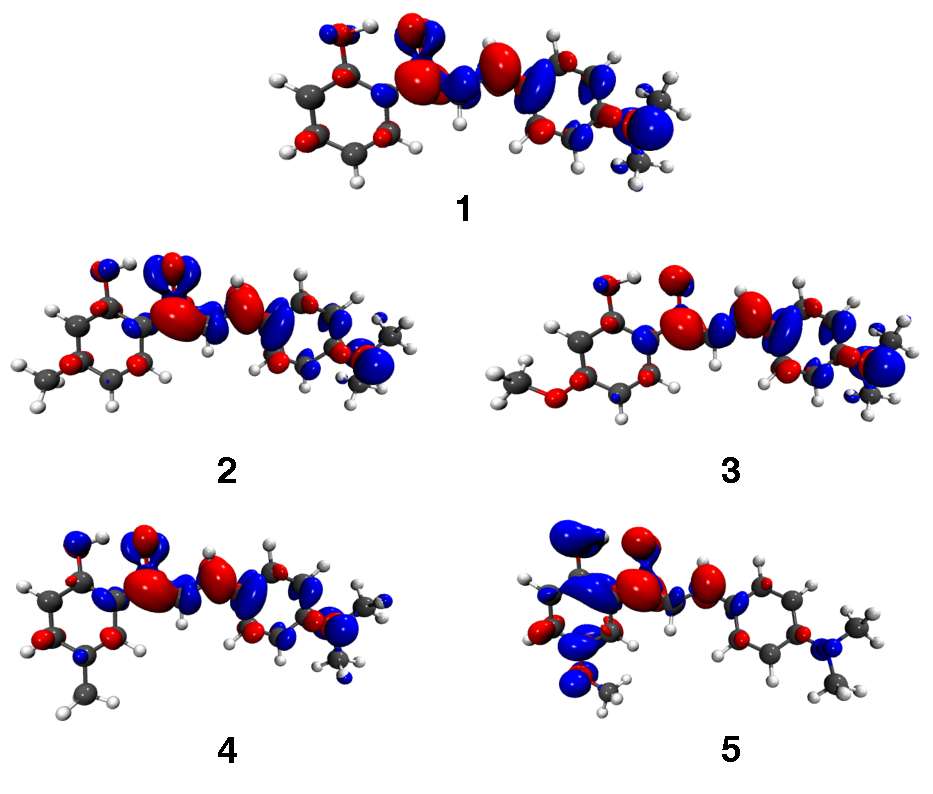
\includegraphics[width=0.8\linewidth]{3nonradiativedecay/HC_Vac_Densities.pdf}
  \caption[Electron density difference maps]{Electron density difference maps (\sone{}-\szero{}) for \textbf{1}-\textbf{5}, showing electron density loss in the ground state (blue) and gain in the excited state (red), calculated at CC2/def2-TZVP level of theory.}
  \label{figure: HC_Vac_Densities}
\end{figure}

Comparing the performance of ADC(2) and CC2 methods, when the same basis set is used (def2-TZVP), ADC(2) vertical excitation energies are about 0.1 eV deviated to the red with respect to the CC2 values. In the case of ADC(2), the def2-SV(P) basis set shifts the energies to the blue in about 0.1 eV. With this basis set there is mixing of the \sone{} and \stwo{} states, where \stwo{} borrows intensity from \sone{} due to  \pipistar{} and \npistar{} mixing, which is present in CC2 but to a lesser degree. The simulation of the spectra, Figure \ref{figure: HC_spectra_ADC}, using a Wigner-distributed sample of nuclear configurations at the ADC(2)/def2-SV(P) level of theory shows a red shift of 0.1-0.2 eV due to vibrational broadening. Similar shifts are expected for all levels of theory.
\begin{figure}[t]
\centering
  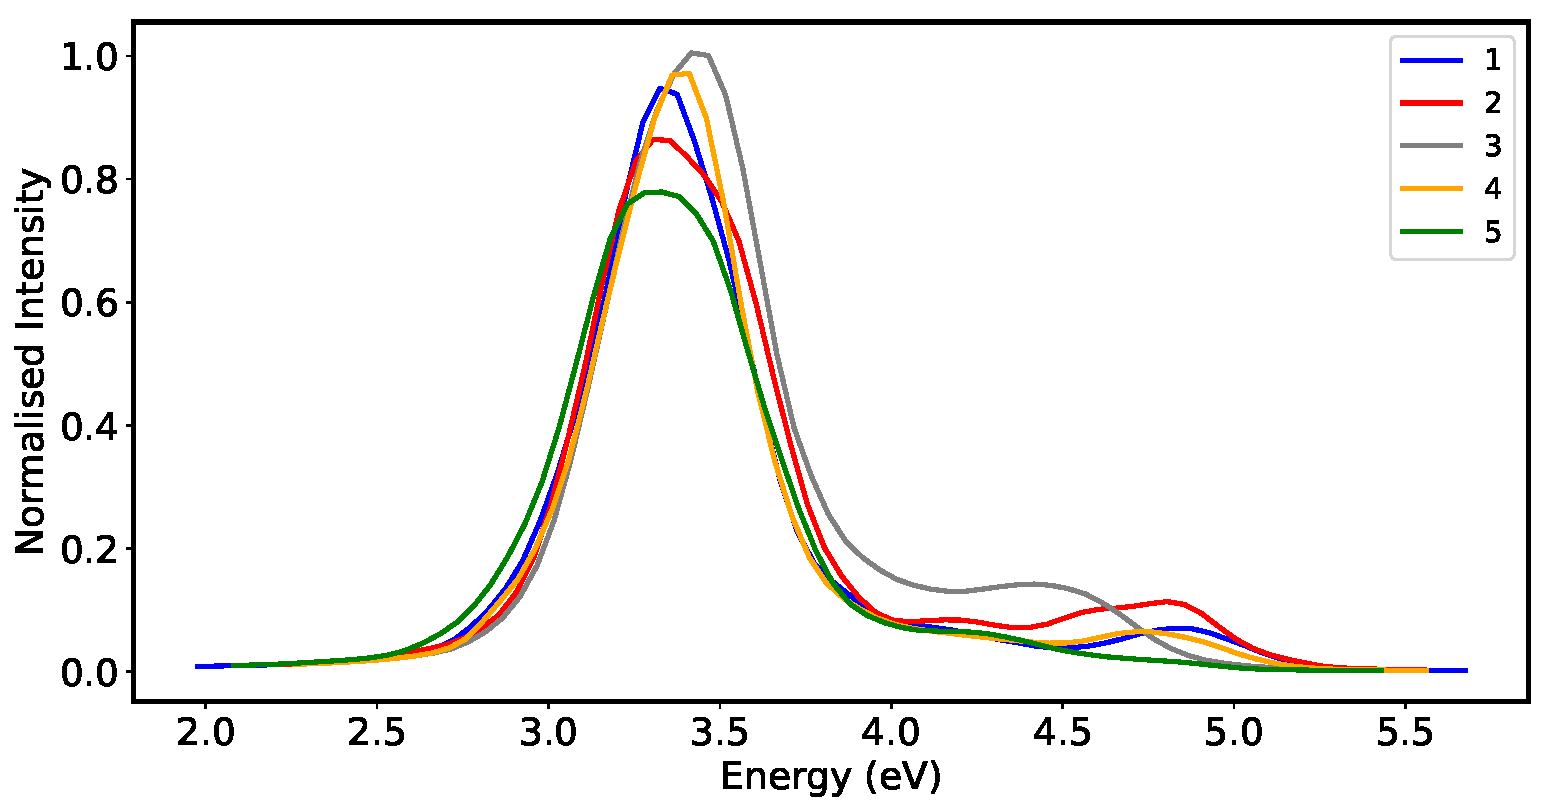
\includegraphics[width=0.8\linewidth]{3nonradiativedecay/HC_Spectra_ADC2.pdf}
  \caption[Simulated absorption spectra of \textbf{HC1}-\textbf{5}]{Simulated absorption spectra of \textbf{HC} \textbf{1}-\textbf{5} at ADC(2)/def2-SV(P) level of theory.}
  \label{figure: HC_spectra_ADC}
\end{figure}


\subsection{Excited State Minima}\label{section: NRdecay_Minima}
Minima in the first excited state for all compounds were optimised using ADC(2) and CC2 methods. The respective energy levels are depicted in Figure \ref{figure: HC_Energy_Levels}. An \ac{EDG} in \textit{meta} (\textbf{2} and \textbf{3}) has a negligible effect on the energies of \Estar. However, if the substituent is in \textit{para} (compounds \textbf{4} and \textbf{5}), no stable \Estar{} minimum can be located. For \textbf{1}-\textbf{3}, relaxation to a local minimum in \Estar{} is \textit{via} intramolecular rotation. To describe this mode, the torsional rotation angle $\theta_{tor}$ is defined in Figure \ref{figure: H_CC2_LIIC_Scan}.

Two \Estar{} minima can be found depending on the direction of rotation and in the case of \textbf{1}, both minima are energetically equivalent. For \textbf{1}-\textbf{3}, the energy difference between these minima is very small ($<$ 0.01 eV) and the two minima (forward or backwards rotation) can be considered degenerate. Torsion through 180\textdegree{} results in cis-trans isomerisation, with the trans isomer about 1 eV less stable than cis in \sone (at ADC(2), Figure \ref{figure: HC_1_Energylevels_ADC2}). Consequently, full cis-trans isomerisation is unlikely. 

At the \Estar{} minimum  $\theta_{tor}$ = 44\textdegree{} for \textbf{1}, resulting in  a stabilisation of approximately 0.54 eV with respect to the FC state. Compounds \textbf{2} and \textbf{3} pass through similar minima, with $\theta_{tor}$ = 46\textdegree{} and 54\textdegree{} respectively. Potential energy curves and our nonadiabatic dynamic simulations show that ESIPT from this geometry is improbable. Therefore when occupied the \Estar{} minimum acts as a sink for the wavepacket to prevent \ac{ESIPT}, as confirmed by Zahid \textit{et. al} experimentally.\cite{Zahid2017} The emission energies from the \Estar{} state for \textbf{1}, \textbf{2} and \textbf{3} are 1.63, 1.59, and 1.46 eV respectively, but with negligible oscillator strength.

In the \Kstar{} state, where the proton has migrated, the system relaxes \textit{via} intramolecular rotation about $\theta_{tor}$. Two minima with very similar energies can be also located depending on the direction of rotation. The $\theta_{tor}$ value ranges between 40\textdegree{} and 60\textdegree{}. These minima are about 1 eV below the excitation energy corresponding to the FC geometry, and are more stable than \Estar{} minima. As such a bias towards the ESIPT mechanism can be expected, whilst the relative stabilisation with respect to the \sone{} energy for the FC geometry is quite similar for all the derivatives (about 1 eV). The emission from \Kstar{} is in the range of 0.7-1.0 eV for all molecules, but has negligible oscillator strength. \sone{} energies (for \Kstar{} and \Estar) with ADC(2) method are in good agreement the obtained with CC2 (within the 0.1-0.2 eV range). At the same time, ADC(2) destabilises the K ground state with respect the CC2 method. This behaviour has consequences for the optimisation of MECI and the description of the \sone/\szero{} crossing seam using the ADC(2) method, which are discussed in the next section.

\subsection{Relaxation Channels}\label{section: NRdecay_Channels}
\begin{figure}
\centering
  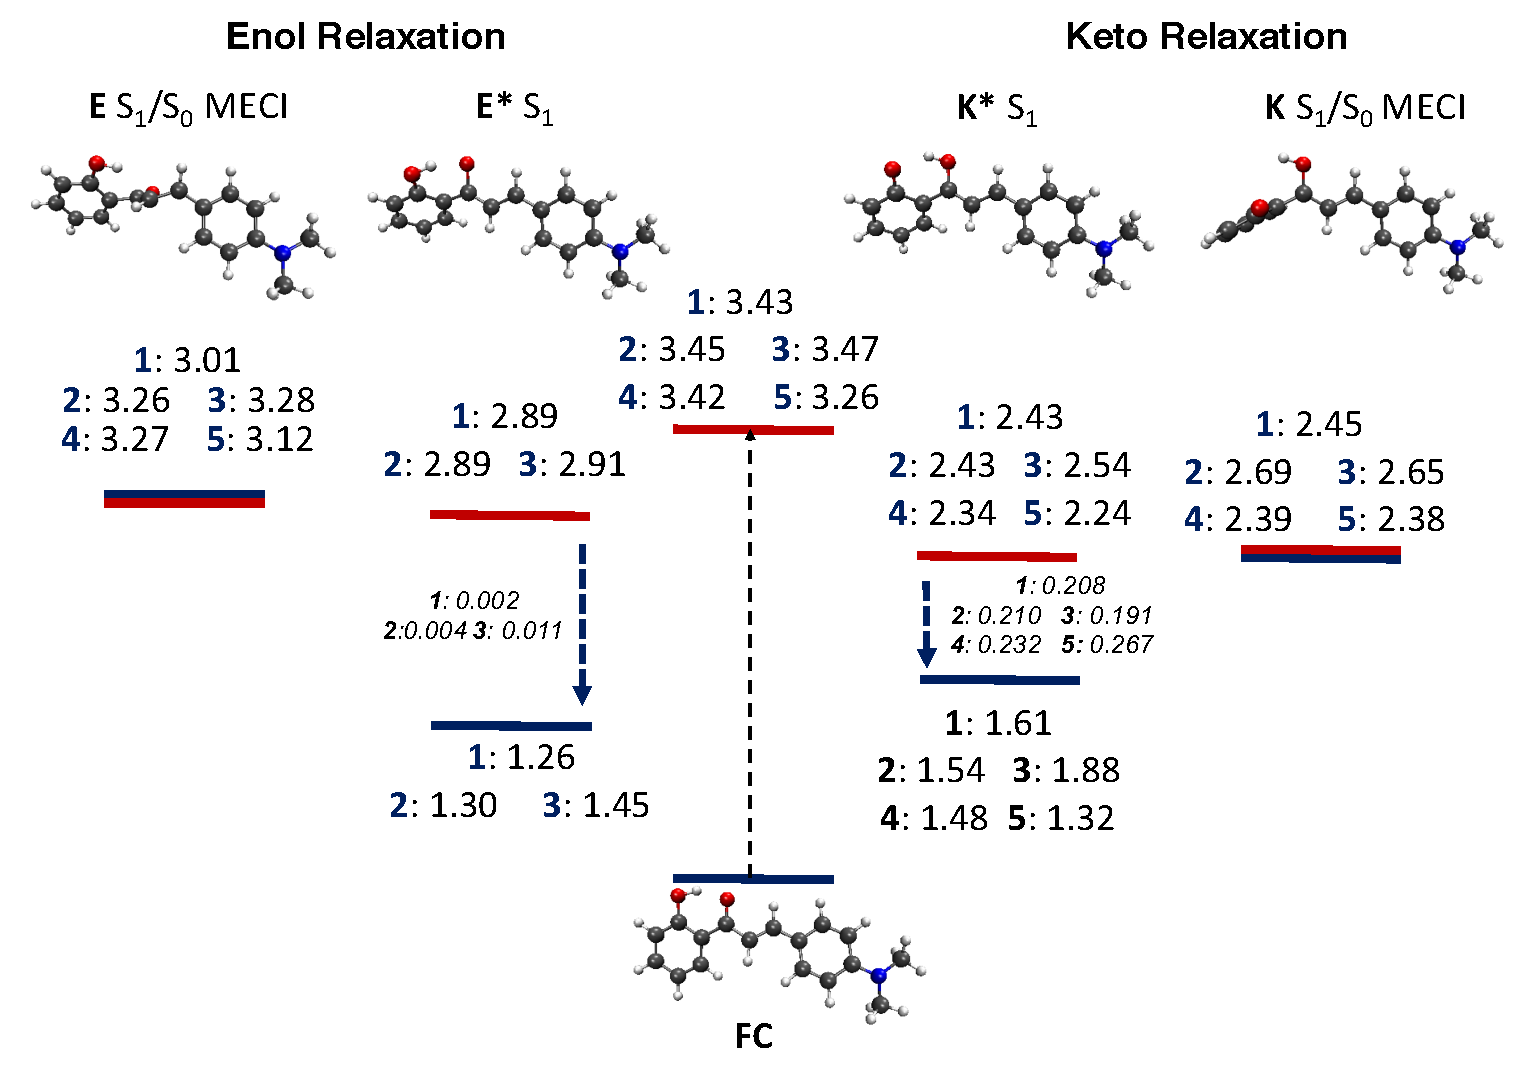
\includegraphics[width=0.9\linewidth]{3nonradiativedecay/HC_Energy_Levels.pdf}
  \caption[\textbf{HC} energy levels]{Relative energies (in eV) for all derivatives calculated at CC2/def2-TZVP level of theory. In all cases, the energy of the ground state was taken as reference.}
  \label{figure: HC_Energy_Levels}
\end{figure}
From the Franck-Condon state, the wavepacket can relax through the enol channel to the \Estar{} minimum, or the ESIPT channel to the \Kstar{} minimum. These two competing channels are depicted in Figure \ref{figure: HC_Energy_Levels}. In each channel, the \ac{MECI} was located to determine the feasibility of nonradiative decay \textit{via} a nonadiabatic crossing. For \textbf{1}, the \ac{MECI} geometries were optimised with CC2 methods using the def2-SV(P) and def2-TZVP basis sets. For comparison, the conical intersections were also located with CASSCF(12,11)/6-31G(d) and CASSCF(14,13) levels of theory. The geometry of the \Kstar{} \sone/\szero{} \ac{MECI} obtained with the CC2 method is in very good agreement with that obtained with CASSCF, $\theta_{tor}$=88\textdegree{} (89\textdegree{} with CASSCF method). The RMSD deviation between the two geometries is just 0.08 \AA. The geometries obtained with both basis sets are very similar. 

For \textbf{1}, the MECI lies at only 0.02 eV above the \Kstar{} minimum, whilst the substituents slightly increase the energy of the MECI (0.1-0.2 eV) in \textbf{2}-\textbf{5}. Nevertheless, the MECIs remain accessible during the relaxation. To determine if any barriers exist between the \Kstar{} minimum and the MECI, we optimise the intermediate states of a linear interpolated pathways, fixing $\theta_{tor}$, at CC2/def2-TZVP level of theory for \textbf{1}. This is shown in Figure \ref{figure: H_CC2_LIIC_Scan}. At the \Kstar{} minimum, $\theta_{tor}$ = 50\textdegree, and further 30\textdegree{} rotation takes the molecule to the intersection seam. In this region of the potential energy surface, the \sone{} energy does not change significantly with $\theta_{tor}$, which can be associated with an extended crossing seam as previously described by Robb \textit{et al}. in an analogous ESIPT system.\cite{Paterson2005}

\begin{figure}[t]
\centering
  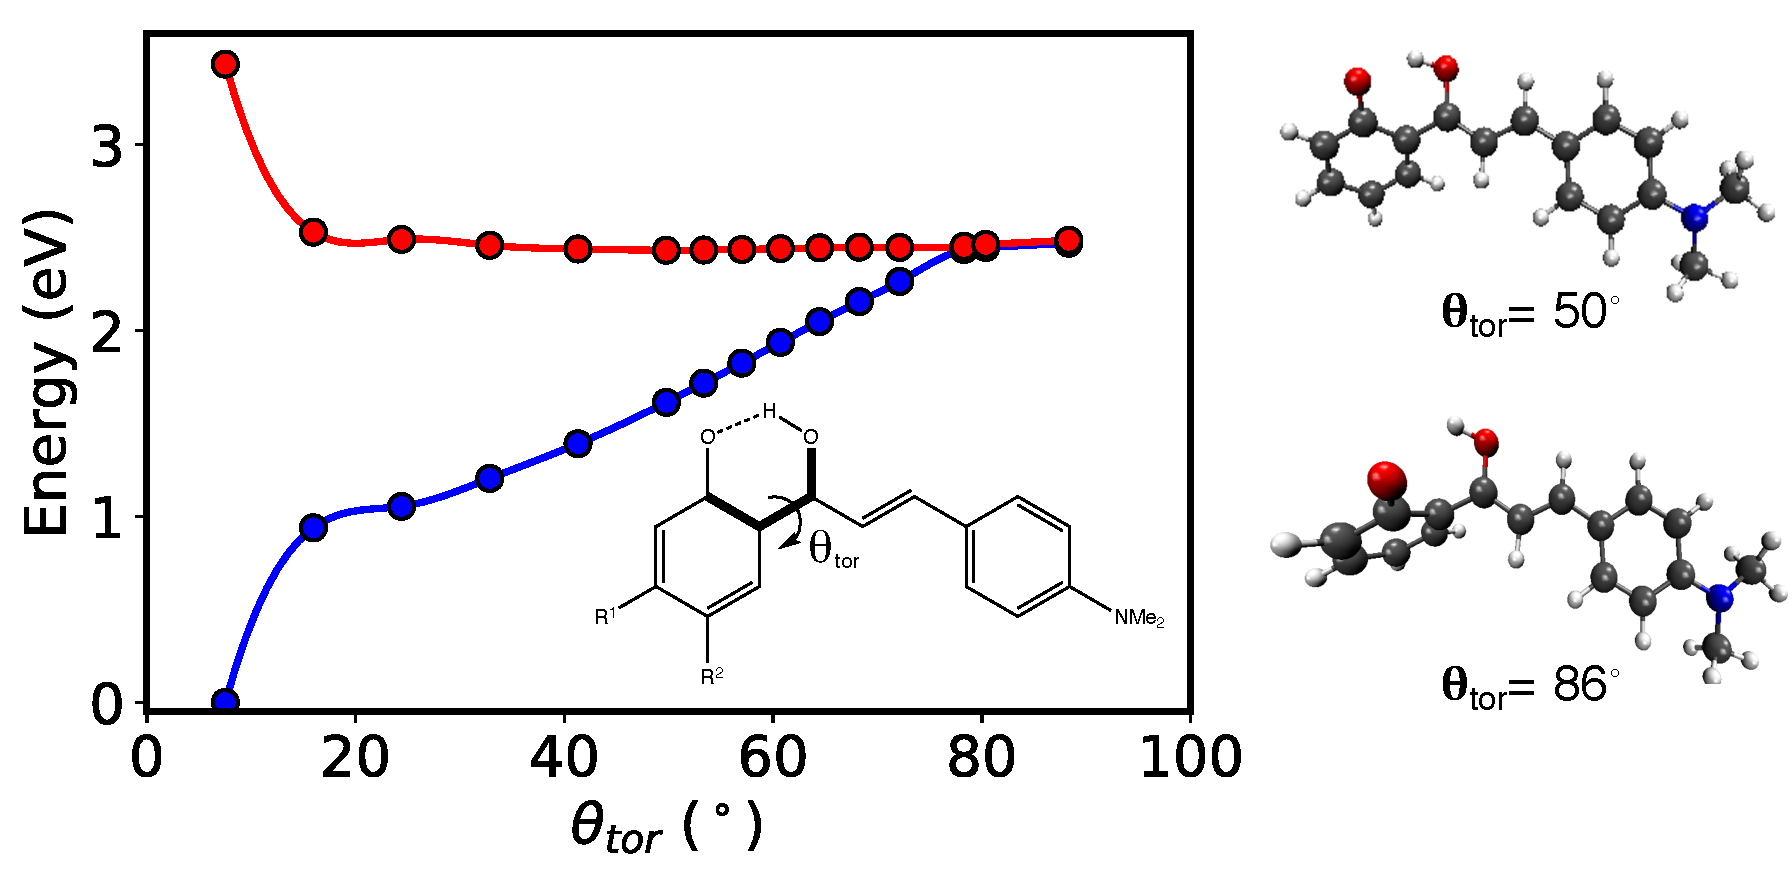
\includegraphics[width=0.9\linewidth]{3nonradiativedecay/H_CC2_LIIC_Scan.pdf}
  \caption[Potential energy surface along the relaxation mode $\theta_{tor}$]{Relaxed linear interpolation pathway between the FC state and the MECI. LIIC located six geometries between the FC state  \Kstar{} minimum, followed by LIIC to locate 10 geometries between the \Kstar{} minimum and MECI. All geometries were relaxed at CC2/def2-TZVP level of theory with $\theta_{tor}$ fixed.}
  \label{figure: H_CC2_LIIC_Scan}
\end{figure}

The frustration of intramolecular rotation in the solid state has been hypothesised to prevent access to a conical intersection, resulting in \ac{AIE}. We observe similar results when the dihedral angle is fixed during \Kstar{} optimisation. The linear interpolation potential energy curves show that there is a stable \Kstar{} region for \textbf{1} prior to the conical intersection, where emission could take place in the NIR region if the rotation is strongly hindered. The driving force behind the rotation is potentially the stabilisation of the dipole moment, which increases from 7.73 (\szero{}) to 13.32 D (\Estar) upon excitation. This is reduced to 3.99 D in the twisted conformation.

The static calculations suggest that the dominant relaxation process involves a proton transfer step followed by rotation about $\theta_{tor}$. ESPIT is facilitated by the \Kstar{} minimum, which is more stable than \Estar. Experimentally, \textbf{4} and \textbf{5} do not show fluorescence either in solution or solid state. In the case of the solid state, the lack of fluorescence has been associated with the crystal packing, however these calculations suggest that the character of the substituent might also play a role. This shall be further investigated in the next chapter.

The ADC(2) geometries for the \Kstar{} \sone/\szero{} MECI of all studied compounds show a $\theta_{tor}$ angle significantly deviated from CC2 and CASSCF values, with the crossing seam reached at a much smaller angle . The ADC(2) MECI structures are very similar to the \Kstar{} minima, rotated by a further 10\textdegree{}. This behaviour is associated with the description of the ground state with the MP2 method, which could artificially destabilise \szero{} and thus the \sone/\szero{}  crossing occurs at smaller angles. Similar results were found with def2-SV(P) and def2-TZVP basis sets.

The non-ESIPT relaxation channel is also accessed \textit{via} intramolecular rotation in the \Estar{} state, leading to a second MECI. The stabilisation of these MECI structures involves relaxation through $\theta_{tor}$, which is significantly larger for \textbf{1} with a value of about 124\textdegree{} (144\textdegree{} with CASSCF). For \textbf{1}, we also observed relaxation through the H-C-C-H dihedral angle (88\textdegree{}). For the rest of the \sone/\szero{} MECI structures (\textbf{2}-\textbf{5}), only $\theta_{tor}$ deviates from the plane. For \textbf{1}-\textbf{3}, the \Estar{} MECIs are slightly higher in energy than the \Estar{} minima (0.2-0.3 eV).  Considering the small energy gap and the absence of barriers, the crossing seam region should be accessible. Another mechanism is the direct relaxation to the MECI from the FC geometry, which is the only possibility for \textbf{4} and \textbf{5}, considering the lack of a stable \Estar{} minimum. These calculations show that the competition between the ESPIT and the relaxation to \Estar{} will depend on the substituent. In the case of \textbf{4}-\textbf{5}, a heavy bias towards the ESPIT is expected. Nonadiabatic dynamic simulations confirm this analysis. 
\subsection{Nonadiabatic Dynamics}\label{section: NRdecay_Dynamics}

For these systems, the \sone{} \acp{PES} obtained with ADC(2) are in a good agreement with the CC2 prior to the conical intersection. The greater computational efficiency of ADC(2) over CC2 also makes it attractive for the study of the first steps of the excited state dynamics of \textbf{HC} systems, although the results when the energy of \sone{} and \szero{} converge must be analysed with care. In particular, it is expected that excited state lifetimes may be underestimated. 

Compounds \textbf{1} and \textbf{5} represent the extreme cases, with most significant difference in the electronic structure of the excited states. The dynamics simulations thus use \textbf{1} and \textbf{5} as exemplars, a strategy which will also be used in Chapter \ref{chapter: Inter}.  The \acp{PES} show that rotation around the angle $\theta_{tor}$ is activated during relaxation (in \Estar{} and \Kstar{}). \ac{TSH} allows analysis of the competition between different relaxation pathways and the role of rotation in the mechanism. The first steps of the photorelaxation of \textbf{1} and \textbf{5} were explored using nonadiabatic dynamics considering two excited states (\stwo{} and \sone{}), which are close in energy. The simulations confirm that the main deactivation pathways are associated with relaxation to the \Kstar{} and \Estar{} minima, with both mechanisms involving  rotation about $\theta_{tor}$. The competition between the two relaxation channels strongly depends on the substituent. 

First we analyse the populations and lifetimes of the adiabatic states. The lifetimes of \stwo{} and \sone{} were estimated using a consecutive reaction scheme,
\begin{align*}
\centering
\ce{&S_{2} ->[$K_{1}$]S_{1} ->[$K_{2}$] S_{0}}
\end{align*}

yielding a set of differential equations. 
\begin{equation}\label{equation: s2rate}
    \frac{dS_{2}(t)}{dt}=-K_{1}S_{2}(t)
\end{equation}
\begin{equation}\label{equation: s1rate}
    \frac{dS_{1}(t)}{dt}=K_{1}S_{2}(t)-K_{2}S_{1}t
\end{equation}
\begin{equation}\label{equation: s0rate}
    \frac{dS_{0}(t)}{dt}=K_{2}S_{1}t
\end{equation}

Equations \ref{equation: s2rate}-\ref{equation: s0rate} were integrated using the \texttt{maxima} linear algebra package, whichleads to the following expressions for the populations:
\begin{equation}\label{equation: state_rates}
    \begin{bmatrix}
    S_{2}(t)\\
    S_{1}(t)\\
    S_{0}(t)
    \end{bmatrix}
    =
     \begin{bmatrix}
     S_{2}^{0} & 0 & 0\\
     S_{2}^{0}\frac{K_{1}}{K_{2}-K_{1}} & S_{1}^{0}+S_{2}^{0}\frac{-K_{1}}{K_{2}-K_{1}}& 0 \\
     S_{2}^{0}\frac{-K_{2}}{K_{2}-K{1}} & S_{2}^{0}\frac{K_{1}}{K_{2}-K_{1}}-S_{1}^{0} & S_{2}^{0}+S_{1}^{0}\\
    \end{bmatrix}
    \cdot
    \begin{bmatrix}
    \exp(-K_{1}t)\\
    \exp(-K_{2}t)\\
    1
    \end{bmatrix}
    \end{equation}

The set of equations in \ref{equation: state_rates} was solved for $K_{1}$ and $K_{2}$ using the least-squares method as implemented in the \texttt{optimize.curve\textunderscore{}fit} function of the \texttt{scipy} python package. The global fits are shown in Figures \ref{figure: HC_1_states_dynamics_fit} and \ref{figure: HC_5_states_dynamics_fit} for \textbf{1} and \textbf{5}. In compound \textbf{1}, there is slight population transfer from \sone{} to \stwo{} that is not incorporated in the model and thus decreases the quality of the \sone{} fit. Nevertheless, in both compounds there is fast population transfer from \stwo{} to \sone{}, followed by a longer-lived \sone{} state. In \textbf{1}, the lifetime of 215 fs ($K_{B}$=0.0047 fs\textsuperscript{-1}) dwarfs that of compound \textbf{5} ($K_{B}$=0.0103 fs\textsuperscript{-1}), again underscoring the power of the methoxy group to destabilise the excited state. The longer lifetime of \sone{} for compound \textbf{1} can be attributed to the stability of the \Estar{} channel, where seven trajectories remain beyond the 500 fs simulation time. For compound \textbf{5}, just one trajectory remained active at 500 fs, in the enol state.

\begin{figure}[t]
\centering
  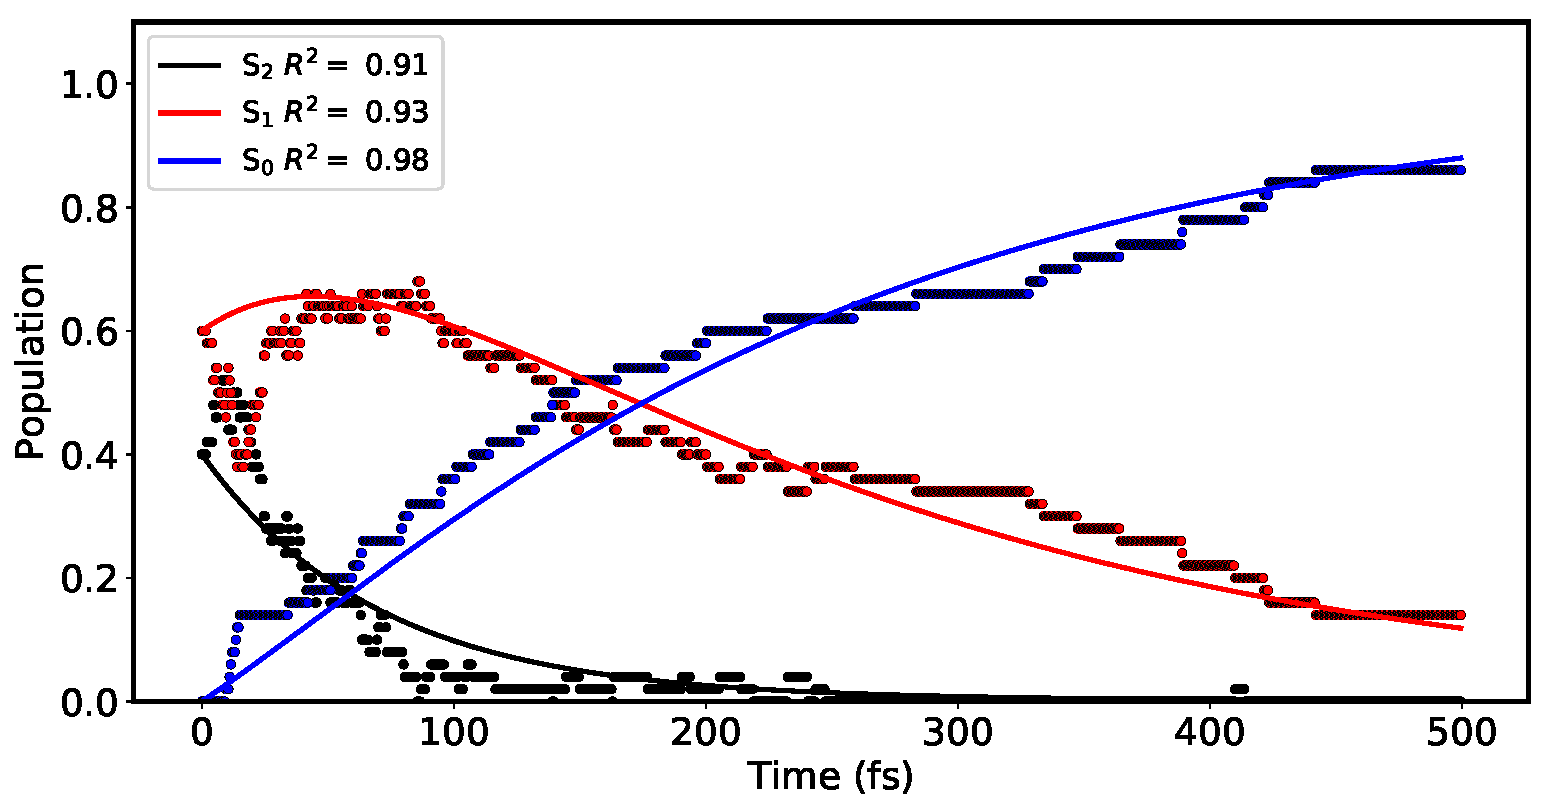
\includegraphics[width=0.9\linewidth]{3nonradiativedecay/HC_1_states_dynamics_fit.pdf}
  \caption[Model of the state decay rates for \textbf{HC1}]{Fit of the rate constants for excited state decay of \stwo{}, \sone{}, and \szero{} for compound \textbf{1}.}
  \label{figure: HC_1_states_dynamics_fit}
\end{figure}

\begin{figure}[t]
\centering
  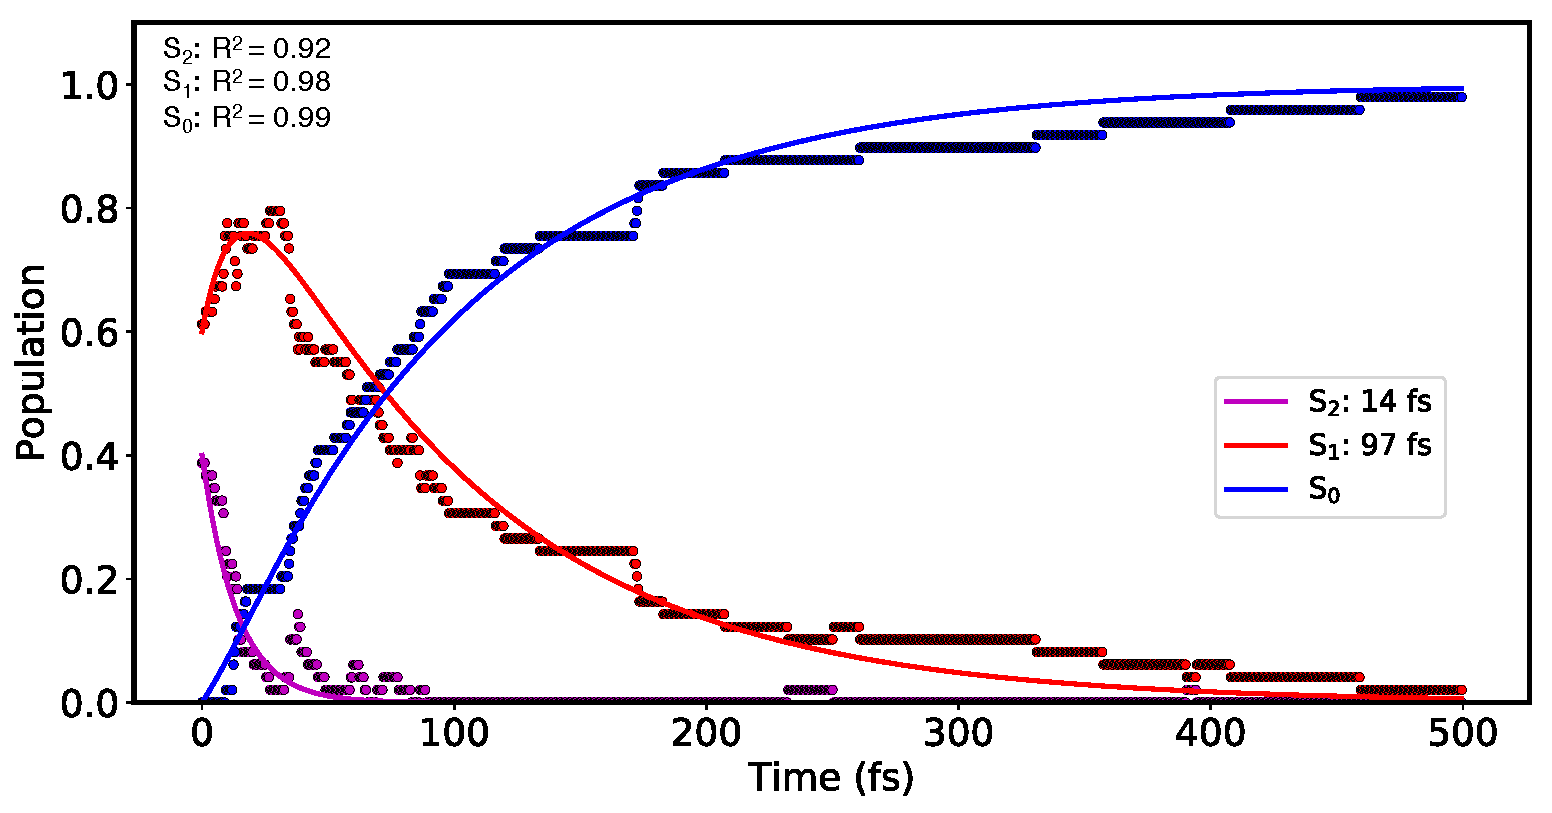
\includegraphics[width=0.9\linewidth]{3nonradiativedecay/HC_5_states_dynamics_fit.pdf}
  \caption[Model of the state decay rates for \textbf{HC5}]{Fit of the rate constants for excited state decay of \stwo{}, \sone{}, and \szero{} for compound \textbf{5}.}
  \label{figure: HC_5_states_dynamics_fit}
\end{figure}

Next we analyse the populations of the two decay channels (\Estar{} and \Kstar{}) by tracking populations of four species in the trajectories: \Estar{}, \Kstar{}, K, and E. Since trajectories were halted if the \sone{}-\szero{} energy gap becomes less than 0.2 eV, the K and E populations are tracked simply by determining if the trajectory is in \Kstar or \Estar{} when the simulation is killed. It is then assumed that population decays through conical intersection to the corresponding ground state in E or K. In a similar vain to the global fits for the adiabatic states, the tautomer lifetimes were modelling using a set of four rate equations:
\begin{align*}
\centering
\ce{&E^{*} ->[$K_{PT}$] K^{*}\\&E^{*} ->[$K_{IC_E}$] E\\&K^{*} ->[$K_{IC_K}$] K}\\
\end{align*}
After integration with the \texttt{maxima} package, the following integrated rate equations were obtained:
\begin{equation}
\mathbf{A}=\mathbf{B}\cdot\mathbf{C}
\end{equation}
\begin{equation}
\mathbf{A}=
    \begin{bmatrix}
    E^\ast(t)\\
    K^\ast(t)\\
    K(t)\\
    E(t)\\
    \end{bmatrix}
    \end{equation}
\begin{equation}
    \mathbf{B}=
    \begin{bmatrix}
    1 & 0 & 0 \\
    \frac{-K_{PT}}{K_{PT}+K_{IC_E}-K{IC_K}} & \frac{K_{PT}}{K_{PT}+K_{IC_E}-K_{IC_K}} & 0\\
    \frac{K_{PT}K_{IC_K}}{(K_{PT}+K_{IC_E}-K_{IC_K})(K_{PT}+K_{IC_E})} & \frac{-K_{PT}}{K_{PT}+K_{IC_E}-K_{IC_K}} & \frac{K_{PT}}{K_{PT}+K_{IC_E}}\\
    \frac{-K_{IC_E}}{K_{PT}+K_{IC_E}} & 0 & \frac{K_{IC_E}}{K_{PT}+K_{IC_E}}
    \end{bmatrix}
\end{equation}
\begin{equation}
    \mathbf{C}=
    \begin{bmatrix}
    \exp(-(K_{1}+K_{2})t))\\
    \exp(-K_{3}t))\\
    1
    \end{bmatrix}
\end{equation}
\begin{figure}[t]
\centering
  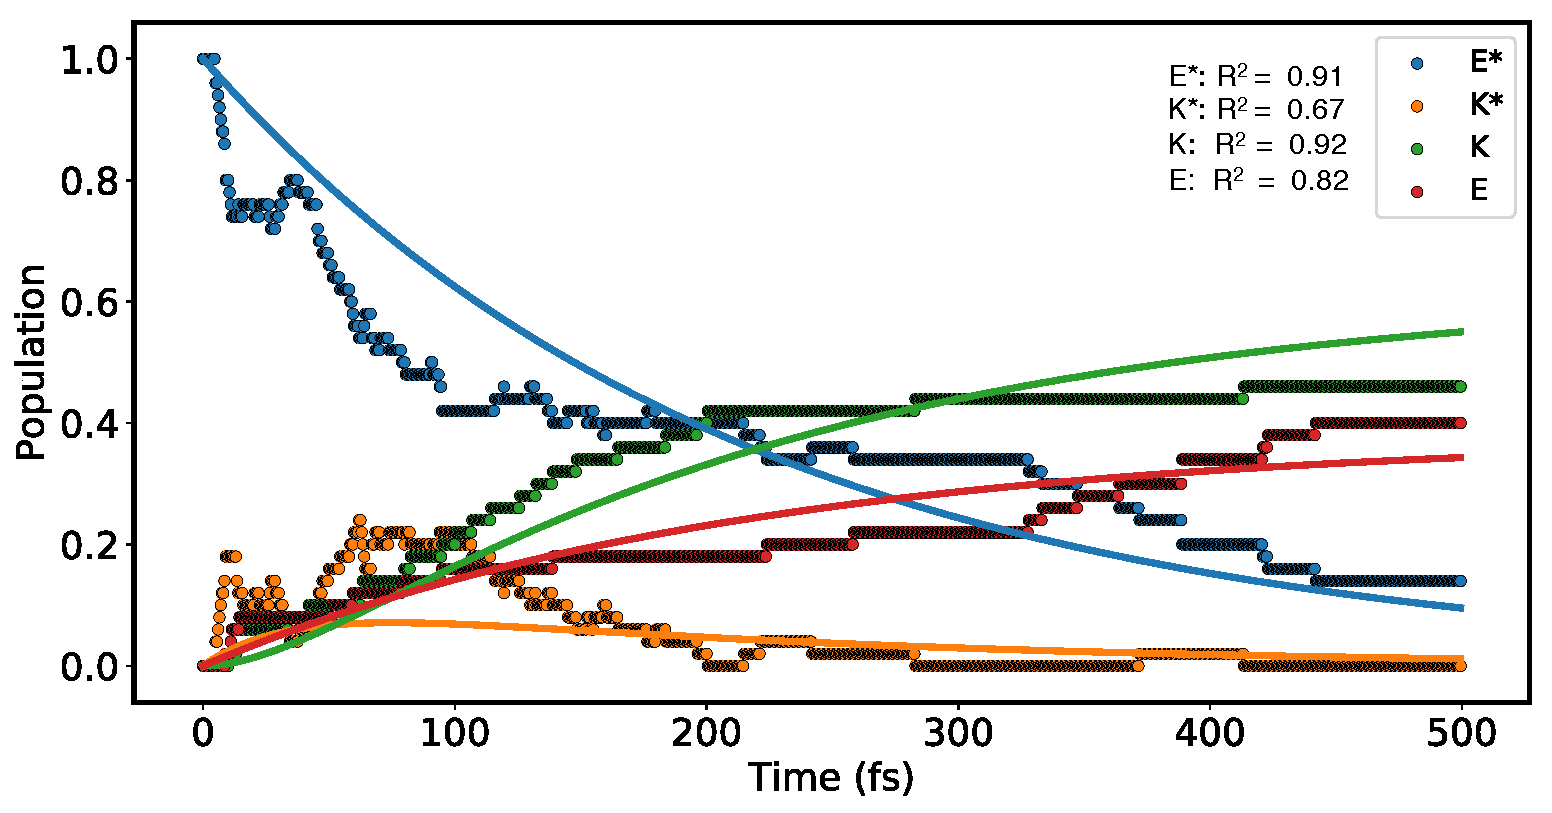
\includegraphics[width=0.9\linewidth]{3nonradiativedecay/HC_1_global_fit.pdf}
  \caption[Global fit for enol and keto states for \textbf{HC1} in nonadiabatic dynamics simulations]{The population of the \Estar{}, \Kstar{}, E, and K states for compound \textbf{1} from \ac{TSH} simulations.}
  \label{figure: HC_1_Global}
\end{figure}
\begin{figure}[t]
\centering
  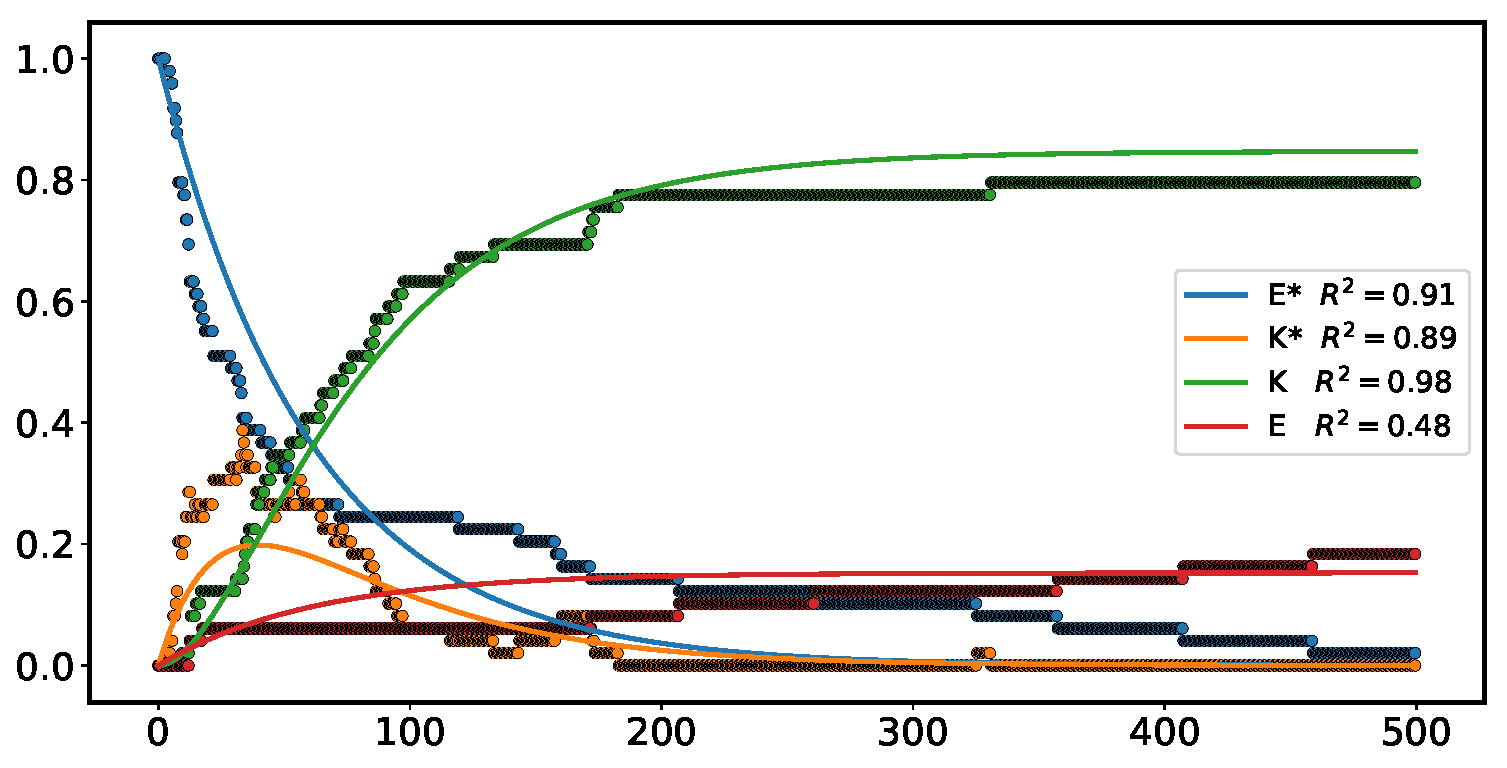
\includegraphics[width=0.9\linewidth]{3nonradiativedecay/HC_5_global_fit.pdf}
  \caption[Global fit for enol and keto states for \textbf{HC5} in nonadiabatic dynamics simulations]{The population of the \Estar{}, \Kstar{}, E, and K states for compound \textbf{5} from \ac{TSH} simulations.}
  \label{figure: HC_5_Global}
\end{figure}

The global fits for the tautomer states are shown in Figures \ref{figure: HC_1_Global} and \ref{figure: HC_5_Global}, and the calculated rates are shown in Table In compound \textbf{1}, $K_{1}$ (the rate of ESIPT) is 2.9 ps\textsuperscript{-1}, which is almost ten-fold slower than in compound \textbf{5}, such is the bias for ESIPT afforded by the addition of the methoxy group. Not captured in the model is the slight oscillatory behaviour between \Estar{} and \Kstar{} populations for compound \textbf{1}, which is not evident in compound \textbf{5}. The internal conversion rates are more similar for the two compounds. These timescales are within the same magnitude of those obtained by Zahid \textit{et. al}, although direct comparison is complicated by the fact that the experimental timescales involve solvation, which is not included in these simulations. 

\begin{table}[H]
\centering
\caption[Obtained rates for decay processes from TSH dynamics for compounds \textbf{1} and \textbf{5}]{Obtained rates for proton transfer, internal conversion in \Estar{} and \Kstar{}, for \textbf{1} and \textbf{5}, in ps\textsuperscript{-1}.}
\begin{tabular}{cccc}
    \hline
     Compound & $K_{PT}$ & $K_{IC_{E}}$ & $K_{IC_{K}}$ \\
     \hline
     \textbf{1} & 2.92 & 1.78 & 28.82 \\
     \textbf{5} & 26.00 & 4.76 & 21.81 \\
     \hline
\end{tabular}
\end{table}

In the case of \textbf{1}, both pathways are similarly populated in the dynamics simulations (\Kstar: 48\%, \Estar: 52\%). The population of the different pathways depends on the initial state. For trajectories started in \stwo{}, the fraction is larger (\Kstar: 60\%, \Estar: 40\%). For \textbf{1}, the significant population of the \Estar{} channel is associated with the stabilisation of the \Estar{} minimum and the lower acidity of the proton due to the electronic density distribution, as shown in Figure \ref{figure: HC_Vac_Densities}. Conversely, compound \textbf{5} shows a significant preference for the \Kstar{} channel, with ESIPT occurring in 80\% of trajectories, showing a similar channel preference regardless of the initial state. The methoxy group results in the increased acidity of the proton and lack of stable \Estar{} minimum, and a heavy bias for the ESIPT channel. This is evident from the fast population transfer of enol to keto in Figure \ref{figure: HC_5_Global}.
%%%%Comment
\begin{comment}
\begin{figure}[H]
\centering
  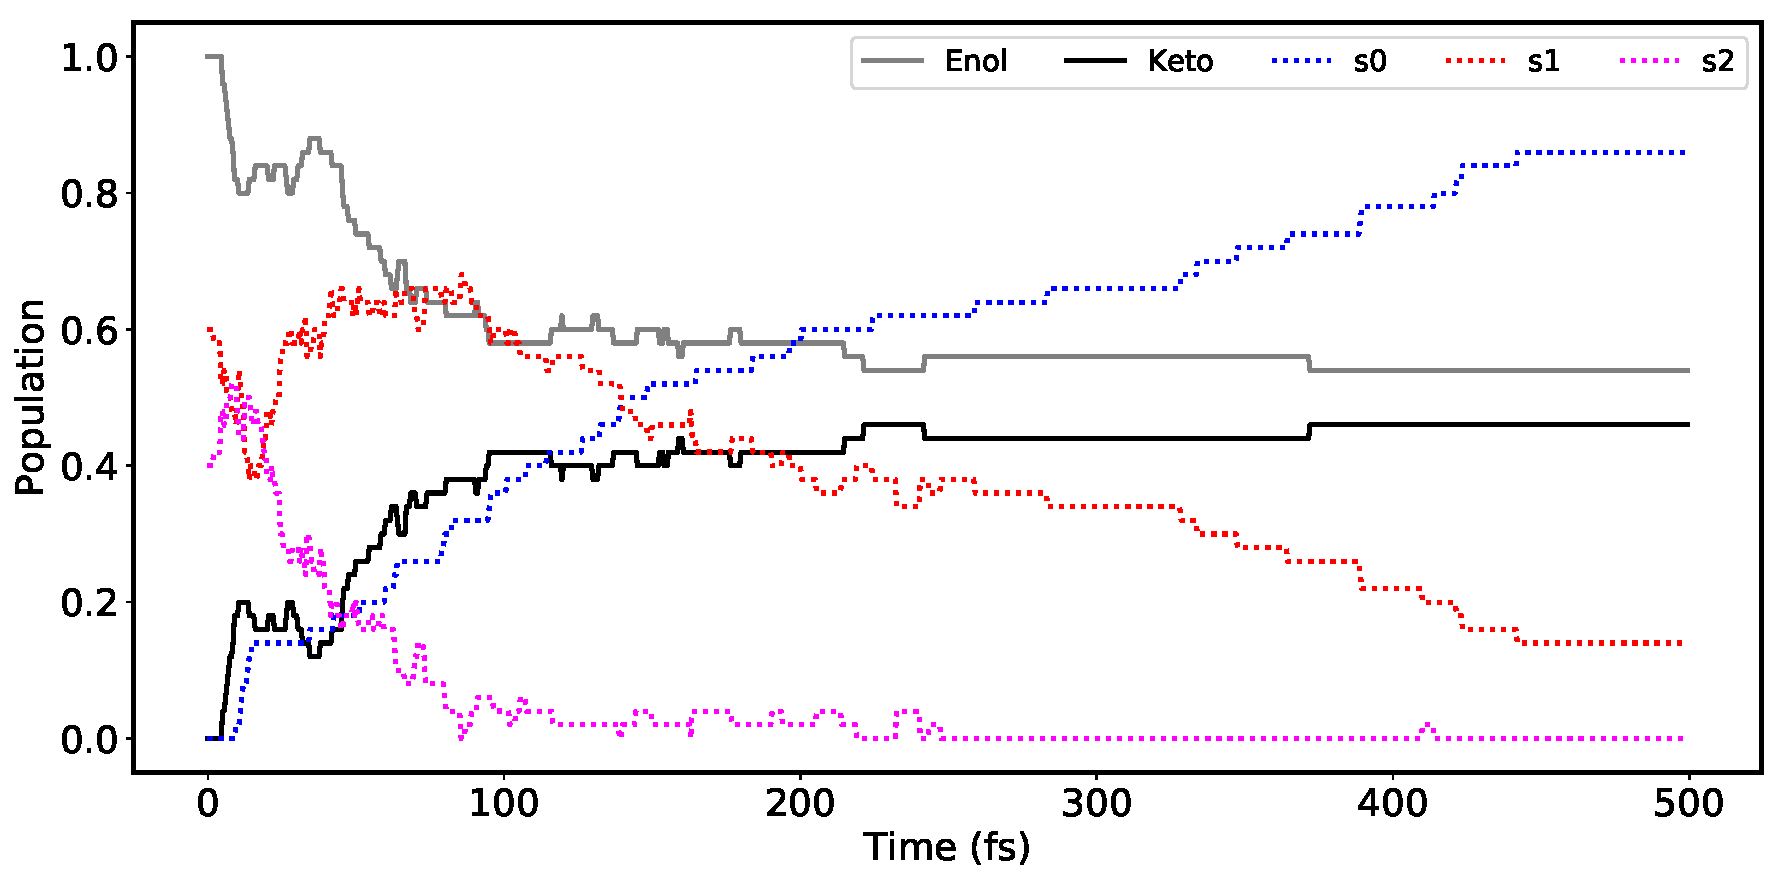
\includegraphics[width=0.9\linewidth]{3nonradiativedecay/HC_1_populations.pdf}
  \caption[Populations of \textbf{HC1} in nonadiabatic dynamics simulations]{The population of the \szero{}, \sone{}, and \stwo{} states for compound \textbf{1} from \ac{TSH} simulations. The population of enol and keto states are also shown.}
  \label{figure: HC_1_Populations}
\end{figure}

\begin{figure}[H]
\centering
  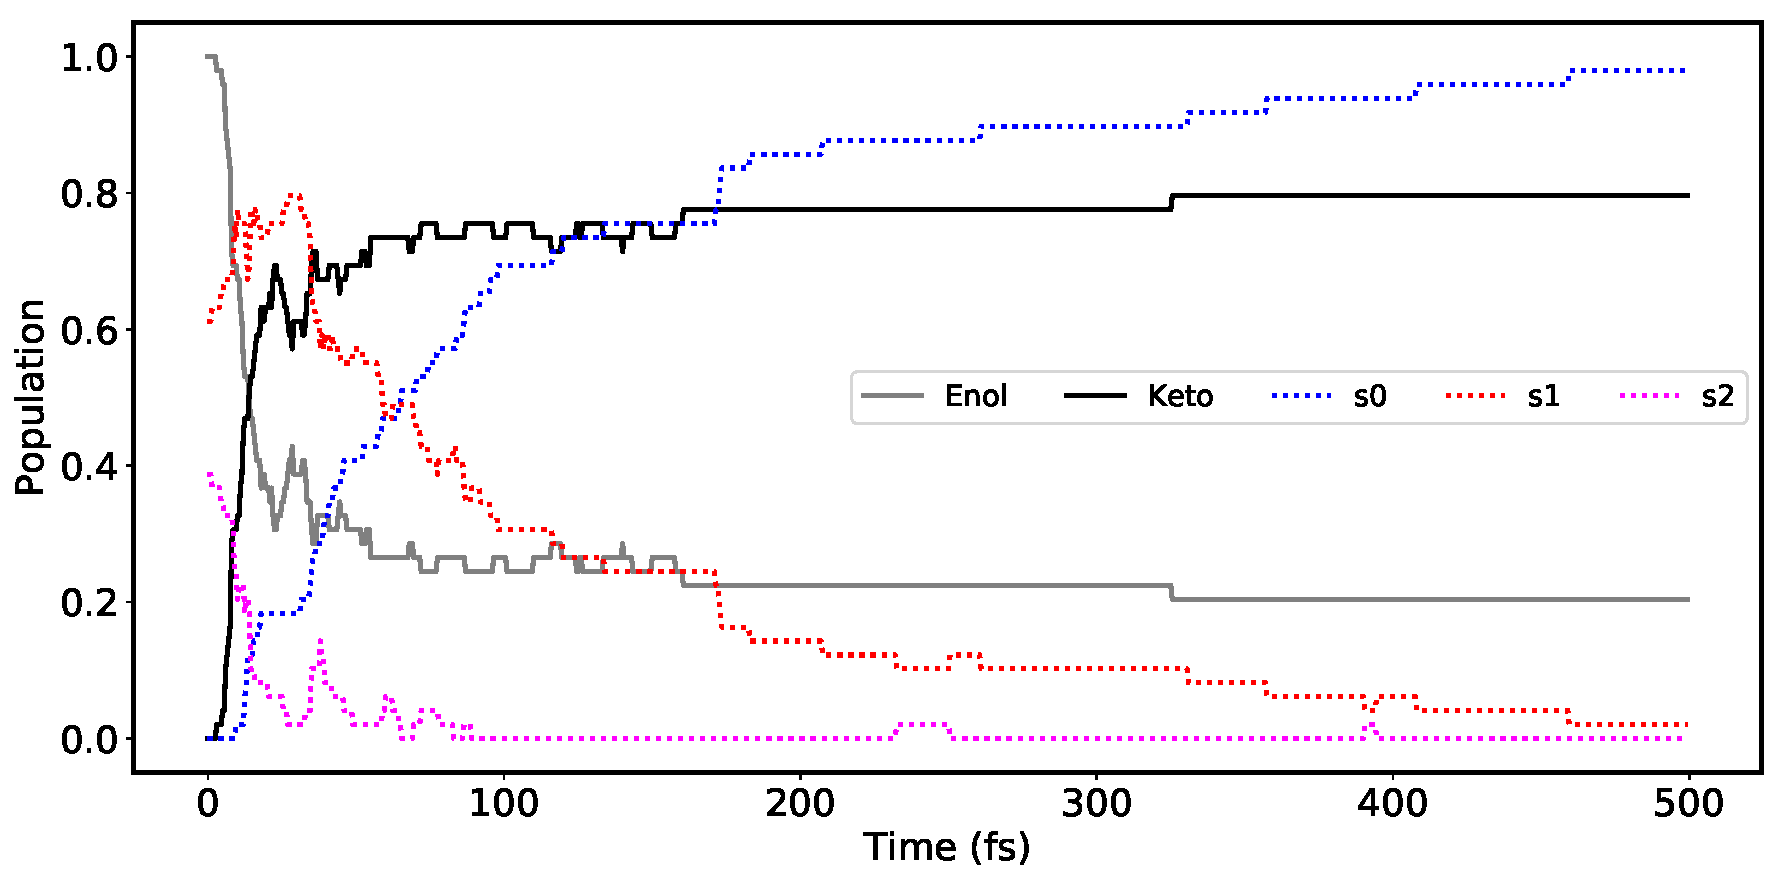
\includegraphics[width=0.9\linewidth]{3nonradiativedecay/HC_5_populations.pdf}
  \caption[Populations of \textbf{HC5} in nonadiabatic dynamics simulations]{The population of the \szero{}, \sone{}, and \stwo{} states for compound \textbf{1} from \ac{TSH} simulations. The population of enol and keto states are also shown.}
  \label{figure: HC_5_Populations}
\end{figure}
\end{comment}
%%%%Comment

To estimate the lifetime of the enol state, the decay rate of \Estar{} was calculated by incorporating both ESIPT and internal conversion into one rate constant. The fit of $K$, the \Estar{} decay rate, for \textbf{1} and \textbf{5} is shown in Figure \ref{figure: HC_Dynamics_Enolfit}. In \textbf{1}, $K=0.0154$ fs\textsuperscript{-1}, giving a lifetime of just 65 fs. For compound \textbf{5} the lifetime is even shorter at just 18 fs. Whilst these times are certainly underestimated, they show the instability of the enol state for \textbf{5} compared to \textbf{1}. While the goodness of fit is reasonable, at 0.74 and 0.81 respectively for \textbf{1} and \textbf{2} (Figure \ref{figure: HC_Dynamics_Enolfit}), the largest error comes from combining the nonradiative decay rate and the ESIPT rate into one decay constant. Furthermore, it can be seen that there are many unphysical step-like features in the populations. Both of these factors are a result of the relatively small number of trajectories run. More accurate lifetimes could thus be attained by running more trajectories and with a higher level of theory to better sample the phase space and allow the separation and estimation of $K_{1}$ and $K_{2}$. However the computational cost associated with this is prohibitive, and for a qualitative description the current method shows the relative differences of the compounds. Besides the elevated computational costs, there are known problems with the stability of CC2 for dynamics.\cite{Plasser2014}

\begin{figure}[t]
\centering
  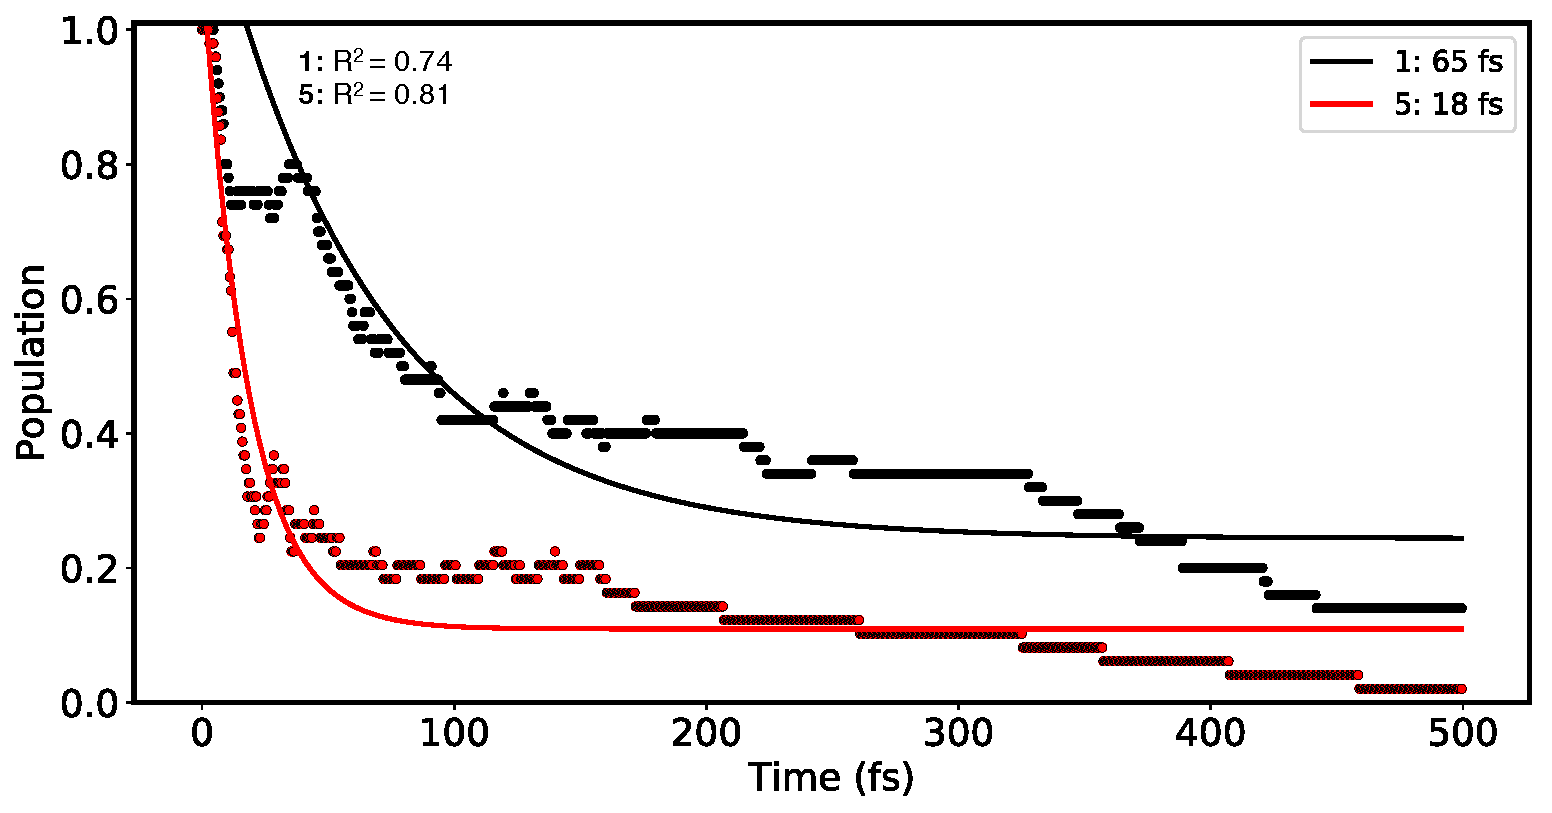
\includegraphics[width=0.9\linewidth]{3nonradiativedecay/HC_dynamics_enolfit.pdf}
  \caption[Estimation of enol decay rate]{Estimation of the enol lifetime for \textbf{1} and \textbf{5} using first-order exponential decay.}
  \label{figure: HC_Dynamics_Enolfit}
\end{figure}




For \textbf{1} and \textbf{5}, the average time for the first proton transfer is 59 fs and 10 fs respectively, with all trajectories exhibiting ESIPT finding the ground state before the maximum simulation time (500 fs). We identify three steps in the ESIPT mechanism:
\begin{enumerate}
    \item Relaxation in the excited state (\Estar{} form)
    \item Proton transfer (ESIPT) 
    \item Relaxation in \Kstar{} followed by internal conversion
\end{enumerate}

These three steps are illustrated for a typical trajectory in panel a) of Figure \ref{figure: HC_1_Trajectories}. During step 1, the angle decreases to $\theta_{tor}$=11\textdegree{} to facilitate the proton transfer in step 2. In some trajectories, the proton oscillates somewhat before transferring. ESIPT in step 2 occurrs at 45 fs. In step 3, the molecule relaxes in the keto form \textit{via} dihedral rotation after which dihedral rotation of 37\textdegree{} results in state convergence after 139 fs, which is underestimated considering the limitations of the ADC(2) method. The region with \sone/\szero{} gap of 0.1 eV is accessed in an average time of 76 fs post-ESPIT for \textbf{1} and 47 fs for \textbf{5}. Considering the features of the PES at ADC(2)/def2-SV(P) level of theory, these times are underestimated with respect to real internal conversion times, but they provide a relative indication of how fast the molecules reach the crossing seam region and the effect of the substituent.
\begin{figure}[t]
\centering
  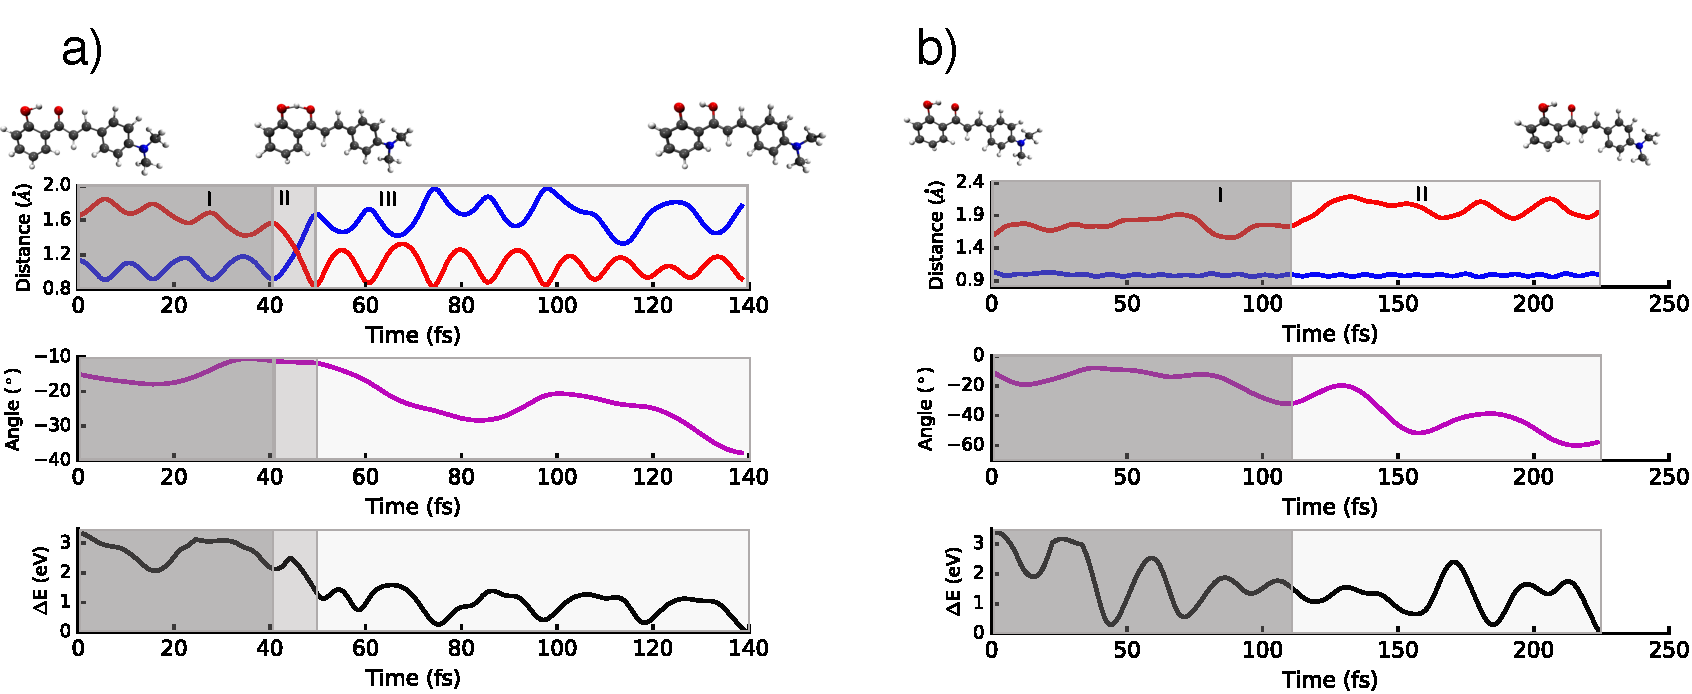
\includegraphics[width=0.9\linewidth]{3nonradiativedecay/HC_1_Trajectories.pdf}
  \caption[Typical trajectories for \textbf{HC1}]{Two exemplar trajectories of compound \textbf{1}. Panel a), left, shows a trajectory undergoing ESIPT, with the associated O-H distances, dihedral angle, and energy gap between \sone{} and \szero{}. The same parameters are shown in panel b) for a trajectory which relaxes in the \Estar{} channel.}
  \label{figure: HC_1_Trajectories}
\end{figure}

Alternatively to ESIPT, the molecule can remain in the \Estar{} state. The mechanism of intramolecular rotation in \Estar{} compromises two steps: 
\begin{enumerate}
    \item Relaxation in the \Estar{} minimum, which is close to the Franck-Condon geometry.
    \item Further relaxation leading to the internal conversion
\end{enumerate}
Both processes involve the rotation around the angle $\theta_{tor}$. 20\% of the trajectories deactivated through this channel did not reach the crossing region within the simulation time. In the case of \textbf{5}, where there is not a \Estar{} minimum close to the Franck-Condon geometry, the molecule relaxes directly to the crossing seam region. On average, the crossing region is reached within  228 fs for \textbf{1} and 241 fs for \textbf{5}. 

In panel b) of Figure \ref{figure: HC_1_Trajectories}, a typical trajectory undergoing \Estar{} relaxation is shown. At 0 fs,  $\theta_{tor}$=-10.5\textdegree{}, and for the first 110 fs of the simulation (step 1), the angle oscillates about the equilibrium value (-11.0\textdegree{} at ADC(2)/def2-SV(P) level of theory). Then, the rotation deviates the phenoxy group from the plane prohibiting ESIPT and the molecule reaches the CI region at 225 fs, with an $\theta_{tor}$=-57.6\textdegree{}. The dynamics support the assertions from the \acp{PES} that proton transfer from the twisted \Estar{} form, with a barrier of 1.2 eV, is improbable. Relaxation in \Estar{} therefore competes with ESIPT in compound \textbf{1} due to the close proximity of a local minimum close to the Franck-Condon geometry. Proton transfer followed by internal conversion is the faster process, with an average time duration of 123 fs, compared to 228 fs for rotation in \Estar{}.

The nonadiabtic dynamic simulations do not allow the prediction of post-internal conversion behaviour, but the analysis of the PES can help understand the following steps in the mechanisms. Post-ESIPT, two relaxation pathways are possible once the MECI is populated. The first completes the four-level photocycle and returns the system to the ground state cis-enol form \textit{via} \ac{GSIPT}. The second continues the rotation about $\theta_{tor}$ to produce the trans-keto form of \textbf{HC}.  Optimisation at the MP2/def2-TZVP level show this structure is more than 1 eV less stable than the ground state, suggesting that \ac{GSIPT} will be preferential. This is shown schematically in Figure \ref{figure: HC_1_Energylevels_ADC2}. The nonadiabatic dynamics simulations clearly illustrate the effect of a strong electron donor in the \textit{para} position on the ESIPT process in \ac{HC}s. The population of the ESIPT channel and rate of proton transfer is greatly increased as is subsequent convergence of the ground and first excited state. 

\begin{figure}
\centering
  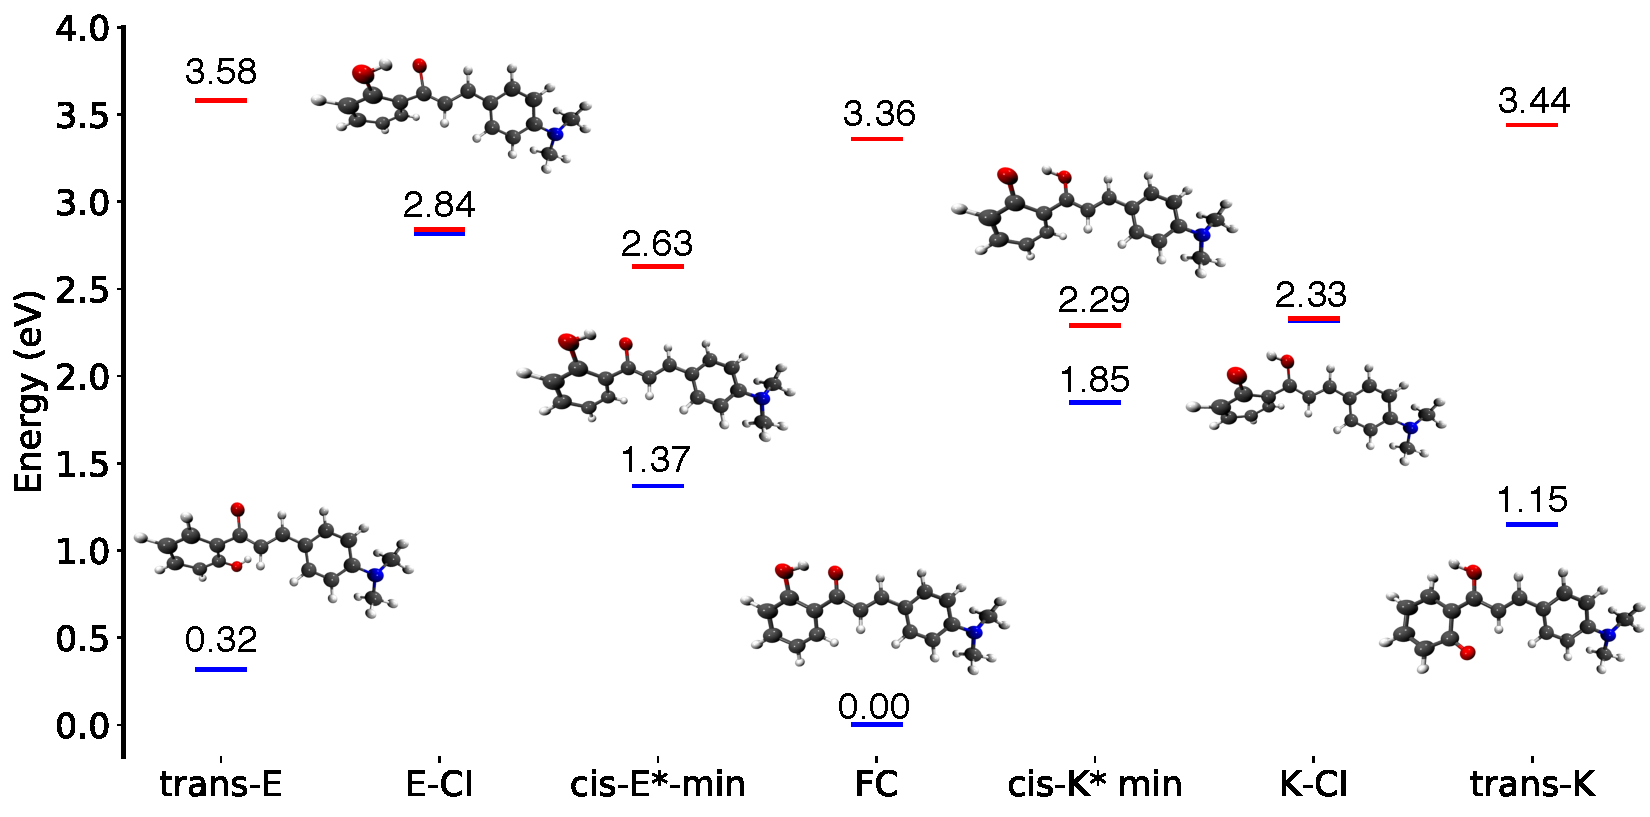
\includegraphics[width=0.9\linewidth]{3nonradiativedecay/HC_1_energylevels_ADC2.pdf}
  \caption[Energies of important optimised states for \textbf{1}]{Energies of important optimised energies on the \ac{PES} of \textbf{1}. Ground states optimised at MP2/def2-TZVP, whilst excited state minima optimised at ADC(2)/def2-TZVP level of theory.}
  \label{figure: HC_1_Energylevels_ADC2}
\end{figure}

\section{Conclusions}\label{section: NRdecay_Conclusions}
In this chapter computational methods have been applied to investigate the photochemistry of five derivatives of \ac{HC}, an ESIPT-active compound with potential application in organic lasers and optoelectronics. Experimental data show that \ac{HC}s are non-emitting in solution and only fluoresce through \ac{AIE}.\cite{Cheng2015} The calculations provide theoretical description of the ESIPT process and subsequent relaxation mechanisms of \ac{HC}s in gas phase, which represents the first step for the understanding of the photochemistry of these systems. 

Through calculation of vertical excitation energies and corresponding absorption spectra, we find that electron donating groups have but a small influence of the absorption characteristics of \ac{HC}. It takes a strong electron donor in the \textit{para} position to alter the vertical excitation energy, on account of the increased conjugated electron density. On the other hand, relaxation back to the ground state is far more sensitive to the electron donating power of the substituent and its positioning on the phenol moiety. Dual-emission is inhibited with an EDG in \textit{para} for \ac{HC}s. This is quite unexpected, with a comprehensive study on the effects of substituents in common ESIPT-compounds finding that electron donating groups in any position favour the \Estar{} form, showing the complex nature of ESIPT chromophores.\cite{Azarias2016}

The ground state is accessible \textit{via} nonradiative channels from both \Estar{} and \Kstar{} states. This analysis has recently been confirmed experimentally,  employing transient absorption and emission spectroscopy, as discussed in Section \ref{section: lom HC spectroscopy}.\cite{Song2018,Zahid2017} \sone/\szero{} MECI structures were found for all compounds, associated with an extended crossing seam. Both mechanisms involve the activation of an intermolecular rotation mode about the $\theta_{tor}$ angle. The competition between \Estar{} and \Kstar{} channels depends strongly on the position and nature of the substituent of the substituent. Proton transfer is more favourable with electron donating groups in \textit{para}, correlating with donating power and increased electron density loss at the phenol oxygen. Nonadiabatic surface-hopping dynamic simulations provide a full picture of relaxation energetics and timescales. 

ESPIT is strongly favoured for \textbf{4}-\textbf{5}, where there are not stable \Estar{} minima. For compound \textbf{5}, the reaction coordinate is completely downhill correlating with intramolecular rotation. The dynamic simulations show a bias towards the \Kstar{} relaxation mechanism. Experimentally, \textbf{4} and \textbf{5} do not fluoresce either in solution or solid state. Cheng \textit{et al.} suggested that for the solid material, this behaviour is related to the crystal morphology.\cite{Cheng2015} Our calculations show that the character of the substituent and the electronic effects in the monomers might also play a role in the mechanism. In the next chapter the knowledge of the electronic properties of \textbf{1} and \textbf{5} shall be used to probe the excited state decay process in the molecular crystal. The question remains of why \textbf{5} is still nonemissive in the solid state whilst \textbf{1} undergoes a stitch-on of fluorescence. To probe this, we shall examine the intermolecular interactions in the molecular crystal and their importance in relation to the electronic properties of the chromophore. 




\chapter[Inter- and Intramolecular Interactions in the Solid State]{Inter- and Intramolecular Interactions in the Solid State}
\label{chapter: Inter}
\begin{figure}[H]
\centering
  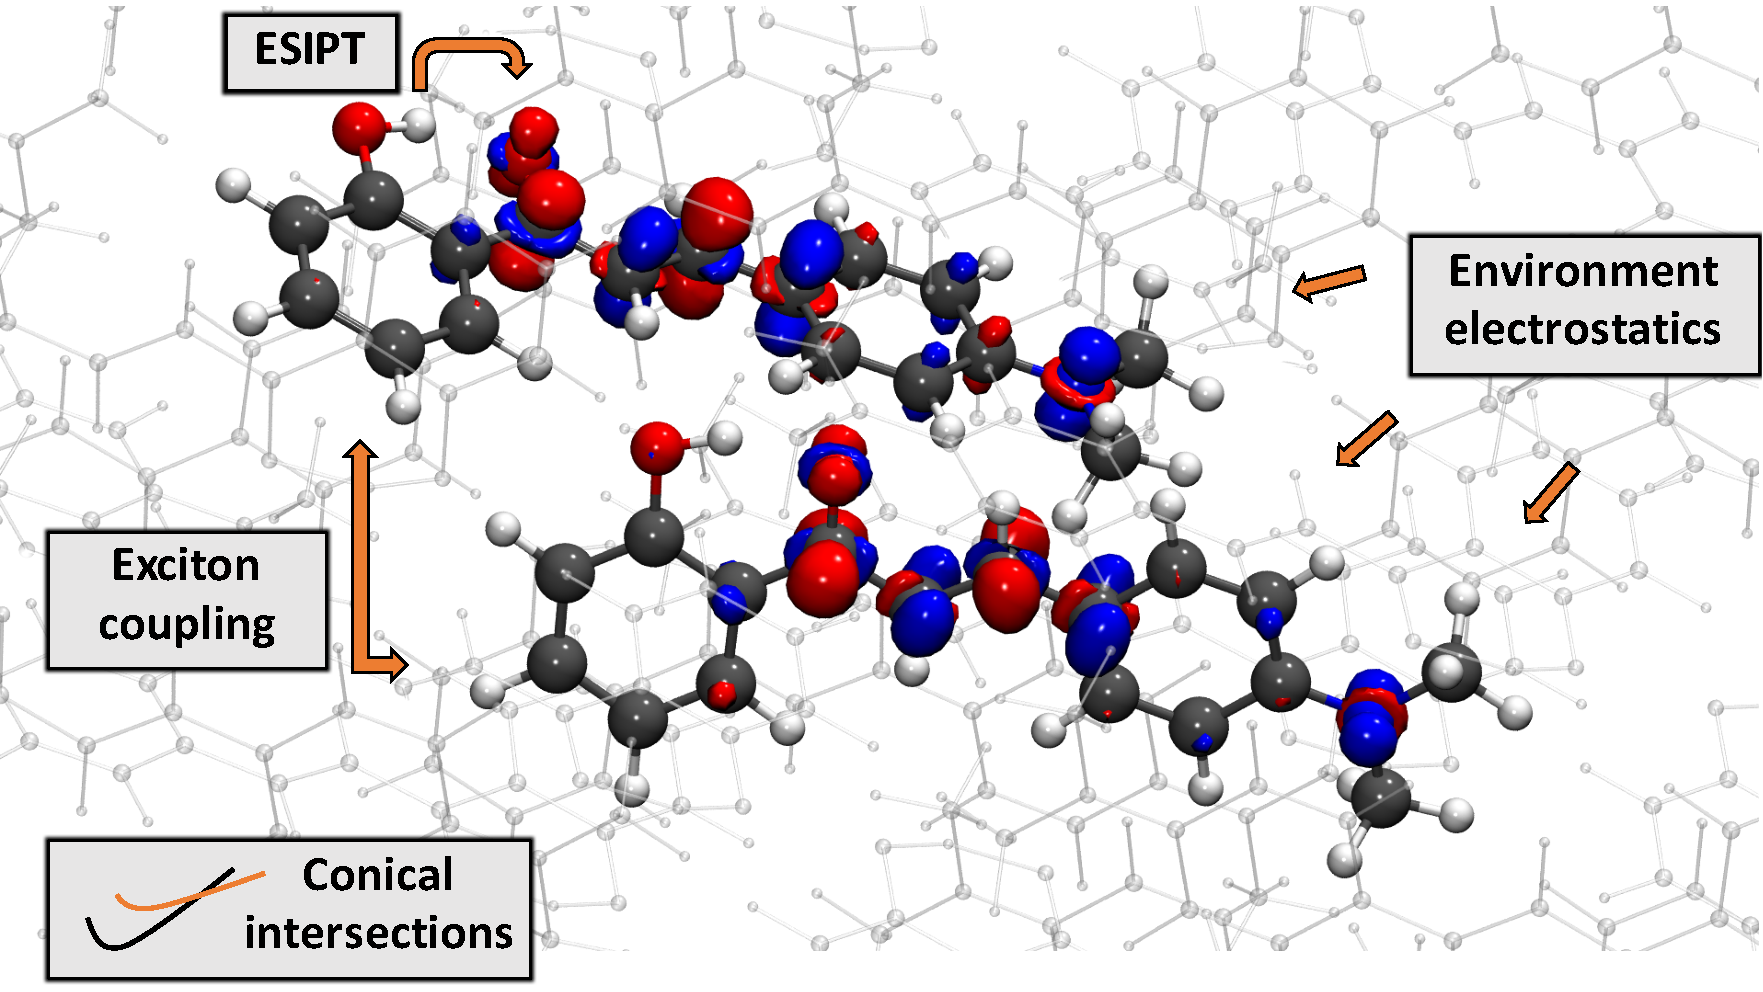
\includegraphics[width=0.6\linewidth]{4IntraInterInteractions/2toc.pdf}
\end{figure}
\section{Introduction}\label{section: Inter_Introduction}
In Chapter \ref{chapter:NRdecay}, the nonradiative decay mechanisms in vacuum were established for the \ac{HC} derivatives \textbf{1}-\textbf{5} (Figure \ref{figure: HC_experimental}). The two extreme cases were compounds \textbf{1} and \textbf{5}, where the methoxy group of \textbf{5} alters the electronic structure of the chromophore. This results in a slight red shift in the absorption, but a more pronounced effect on the relaxation mechanism. Whilst for compound \textbf{1} relaxation through the enol and keto channels is evenly distributed, ESIPT is greatly preferred in compound \textbf{5} due to the increased acidity of the migrating proton. All systems can relax to the ground state \textit{via} an accessible conical intersection in either the enol or keto channel.

In the solid state, compounds \textbf{1}-\textbf{3} undergo \ac{AIE} whereas \textbf{4} and \textbf{5} remain dark. In this chapter, a combination of theoretical models are used to understand the emission properties in the solid state. In particular, we focus how inter- and intramolecular processes determine the emissive properties in the crystal environment. To provide a complete picture of the factors affecting decay mechanisms in these materials, we use a combination of solid state and excited state embedding calculations to systematically account for the different intermolecular interactions present in the molecular crystal. This involves creating cluster models where a central chromophore is treated with a QM electronic structure method and the exterior molecules are described with an \ac{MM} forcefield, in the QM:MM ONIOM approach (Section \ref{section: excited_states_crystals}). As for our nonadiabatic dynamics simulations in Section \ref{section: NRdecay_Dynamics}, in this chapter the two extreme compounds, \textbf{1} and \textbf{5}, shall be used as exemplar systems (Figure \ref{figure: HC_Dimer_Schematic}). In \textbf{1}, chromophores aggregate in a slip-stacking, herringbone structure in an edge to face arrangement. Conversely, in \textbf{5} the dominant configuration is the face to face $\pi$-$\pi$ stacking of chromophores. In Chapter \ref{chapter: Connecting}, the dimer configurations shall be investigated further.

The work herein was published in reference \citenum{Dommett2017b}. The data shall be presented in dedicated sections here, incorporating the Supporting Information, rather than the letter format chosen for publication, although the order of the discussion remains similar. Important to note that while in ref. \citenum{Dommett2017b} the compounds were labelled as \textbf{1} and \textbf{2}, in this work the original numbering of Chapter \ref{chapter:NRdecay} is retained - thus compound \textbf{2} of ref. \citenum{Dommett2017b} is compound \textbf{5} herein. This chapter is organised in the following way. First, the computational methodology is discussed, where we detail the combination of electronic structure methods and embedding models. Second, since the electronic structure method is \ac{TDDFT} for this section, we benchmark vacuum-phase results against those in Chapter \ref{chapter:NRdecay}. Next, the absorption in the solid state is analysed taking into account monomer and dimer chromophores and the excitonic interactions present in the molecular crystal. Excited state minima and conical intersections are then optimised to determine the excited state relaxation mechanism in the molecular crystal and rationalise the observed fluorescence of \textbf{1} and the nonradiative decay of \textbf{5}. Finally, the results are summarised to offer some design rules for ESIPT/AIE systems. All calculations and analyses were performed by myself apart from the Ewald embedding calculations, implemented and performed by Miguel Rivera. All figures are reprinted with permission from ref. \citenum{Dommett2017b}. Copyright 2018 American Chemical Society.
%%%%%%%%%%%%%%%%%%%%%%%%%%%%%%
\section{Computational Methodology}\label{section: Inter_Computional}
%%%%%%%%%%%%%%%%%%%%%%%%%%%%%%
\begin{figure}[t]
\centering
  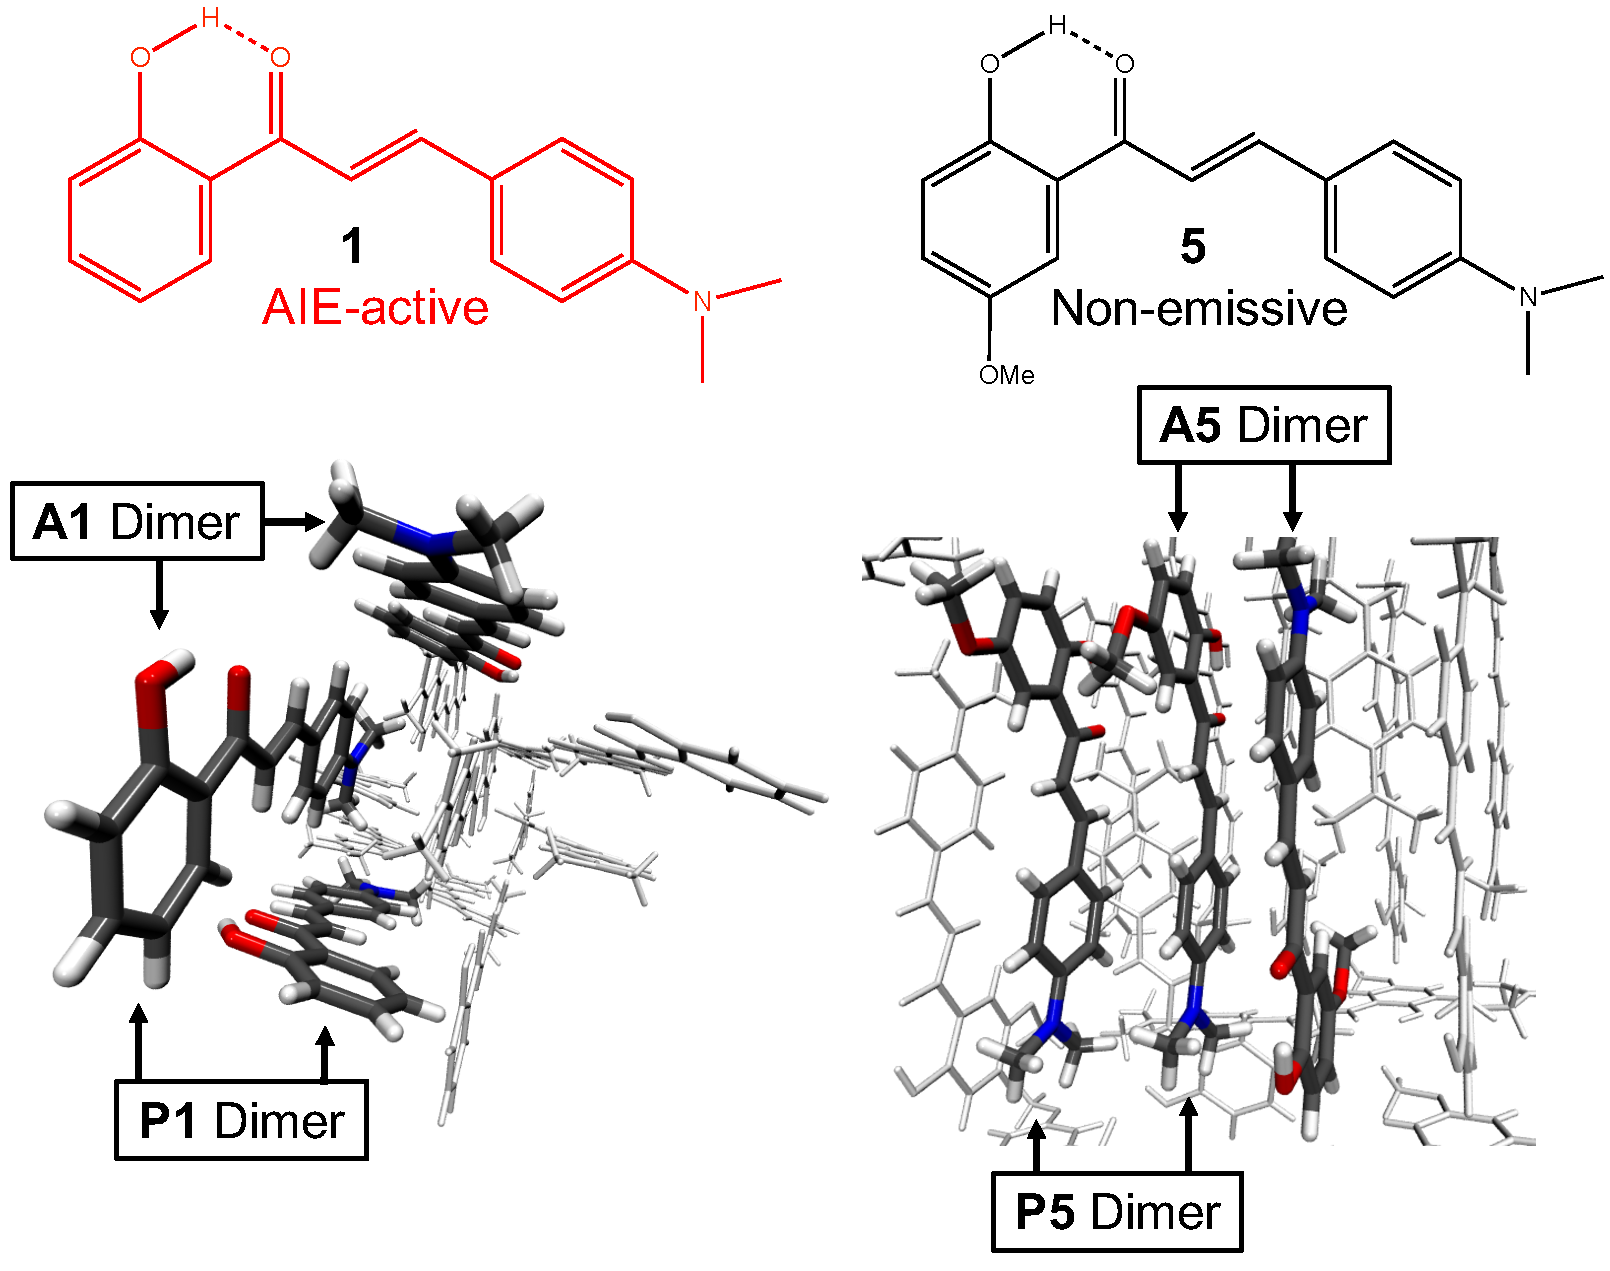
\includegraphics[width=0.9\linewidth]{4IntraInterInteractions/2HC_Schematic.pdf}
  \caption[Molecular, dimer, and crystal structures of \textbf{1} and \textbf{5}]{The molecular and crystal structures of the \textbf{1} and \textbf{5} Compound \textbf{1}, left, displays AIE behaviour, whereas \textbf{5}, right, is nonemissive in both aqueous and solid phases. Also labelled are the parallel (\textbf{P}) and antiparallel (\textbf{A)} dimer configurations.}
  \label{figure: HC_Dimer_Schematic}
\end{figure}
The cluster models of \textbf{1} and \textbf{5} are based on the experimental crystal structures deposited with the CCDC, codes 941991 and 1061608 respectively.\cite{Cheng2015} The crystal structures of \textbf{1} and \textbf{5} were initially optimised using Quantum Espresso in the periodic DFT framework.\cite{QE-2009} Optimisation of each unit cell was carried out with DFT-D2 (PBE) with a plane-wave cutoff of 30 Ry and a Monkhorst-Pack k-point grid of 2x3x2 in accordance with the shape of the unit cell. Clusters of varying size were cut from the DFT-D2-optimised cell for the ONIOM calculations.

The solid state photochemistry of \textbf{1} and \textbf{5} is modelled by applying the ONIOM scheme in a QM:MM protocol using \ac{DFT} and \ac{TDDFT} as the QM electronic structure method.\cite{Byun1999,Frisch2003,Chung2015a} This is an attractive route to efficiently evaluate the mechanism of \ac{AIE}, as the chromophore can be treated within the necessary QM framework whilst the surrounding crystal structure can be evaluated using \ac{MM} methods. For each cluster, the surrounding molecules were fixed in their lattice positions during geometry optimisation of the central chromophore and computed with the AMBER forcefield using ESP charges derived from a vacuum HF/3-21G\textsuperscript{*} calculation of a monomer cut from the crystal structure, allowing electrostatic embedding of a QM-derived electronic density - a scheme we denote AMBER(HF).\cite{Cornell1995}

For all models discussed in the following sections, the focus is four important regions of the \ac{PES}; the Franck-Condon point (FC), enol (\Estar) and keto (\Kstar) minima, and the S\textsubscript{1}/\szero{} MECI. These were established as important points in the vacuum calculations of Chapter \ref{chapter:NRdecay}. Ground and excited state minima and the MECI structures were calculated at the ONIOM($\omega$B97X-D/6-31G(d)):AMBER(HF) level within the DFT and TD-DFT framework. Energies at the ground and excited state minima were recalculated  with the 6-311++G(d,p) basis set. Additionally, RI-CC2/def2-TZVP embedded calculations were performed. The CIOpt algorithm of Levine, Coe and Martinez was again applied to determine the location of the minimal energy conical intersection (MECI) structures.\cite{Levine2008} The nature of the MECIs were confirmed with the CASSCF method in both vacuum and solid state, explained in detail below.

For each of \textbf{1} and \textbf{5}, three ONIOM((TD-)DFT):AMBER(HF) clusters of differing size are evaluated:
\begin{itemize}
    \item \textbf{M7}: all molecules within 7{\AA} of a central monomer chromophore
    \item \textbf{M15}: all molecules 15{\AA} from the central monomer
    \item \textbf{D7}: all molecules within a 7{\AA}-radius from the centroid of a dimer chromophore
\end{itemize}
The cluster models are visualised in Figures \ref{figure: HC_Cluster_Models}-\ref{figure: HC_Dimer_Models}. Two \textbf{D7} dimer models were considered due to the prominence of two dimer arrangements in each of the crystal structure, where monomers are arranged parallel (\textbf{P}) and antiparallel (\textbf{A}). The parallel stacked dimer model is denoted \textbf{D7-P} and the antiparallel configuration is \textbf{D7-A}. These stacking arrangements are shown in Figure \ref{figure: HC_Dimer_Schematic}.

\begin{figure}
\centering
  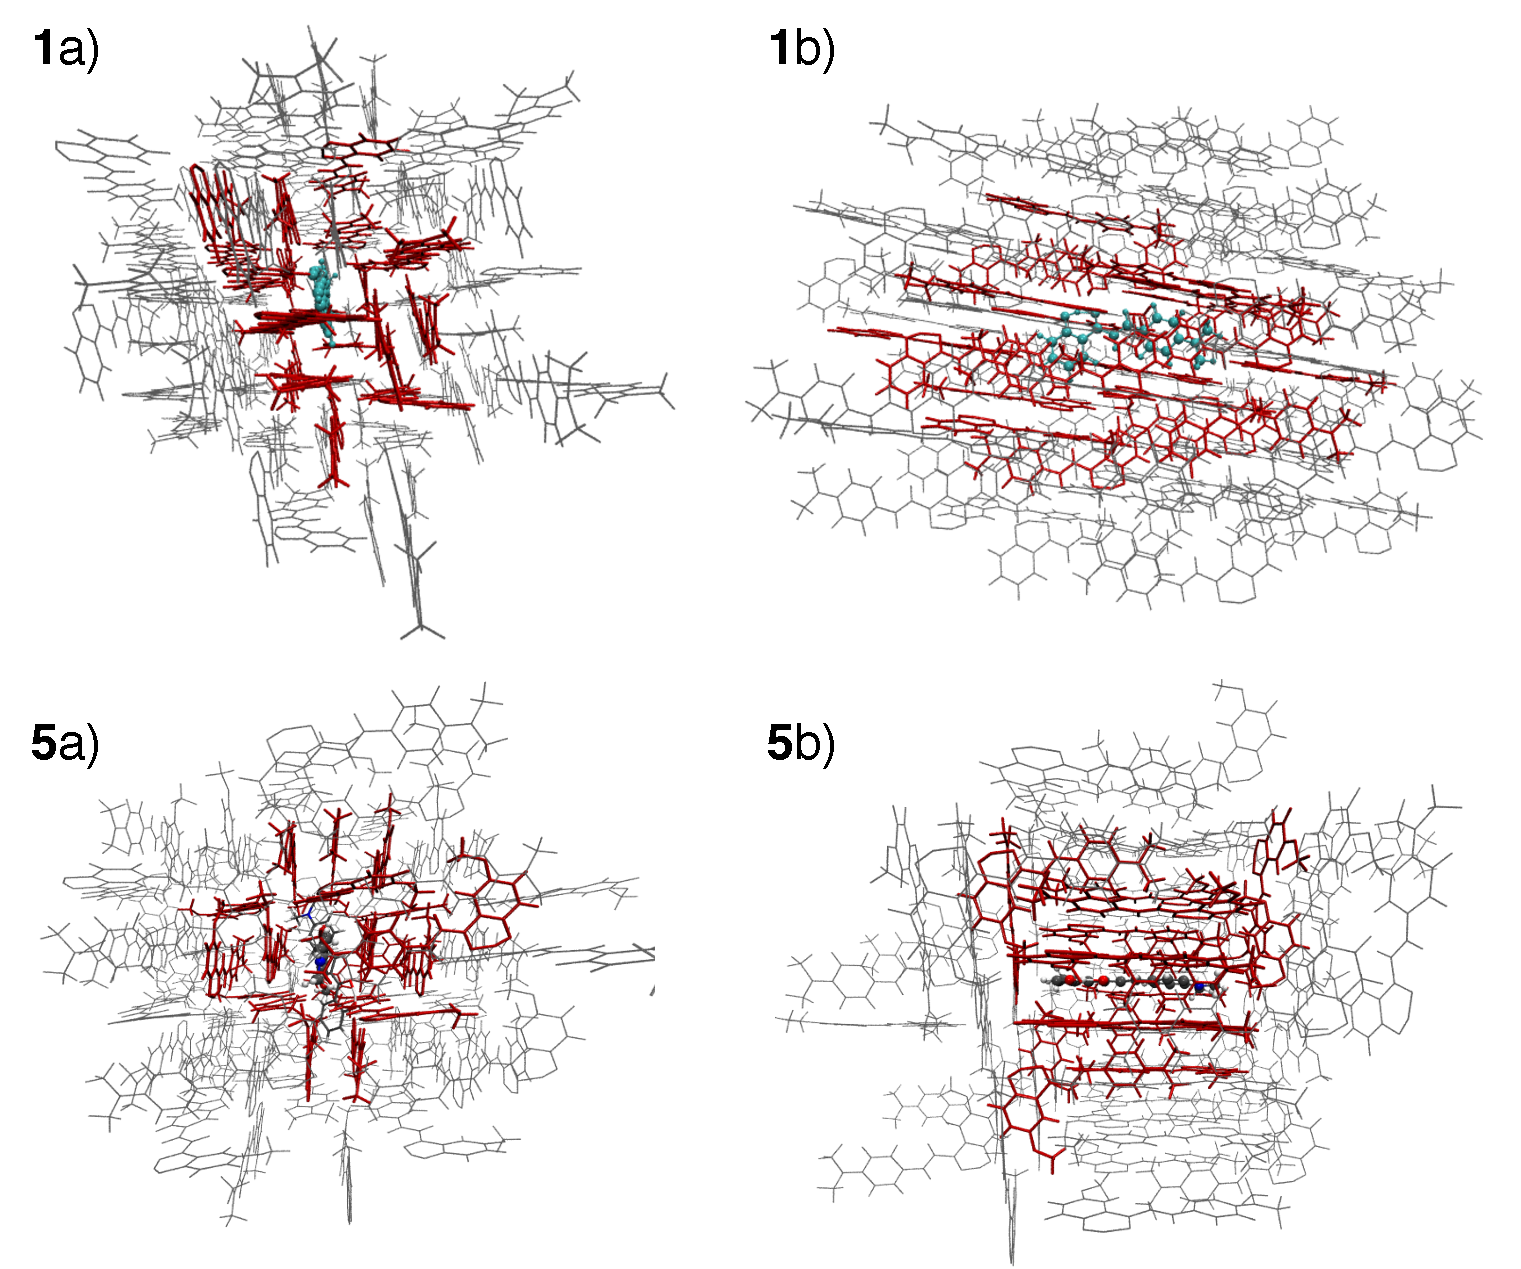
\includegraphics[width=0.8\linewidth]{4IntraInterInteractions/HC_Cluster_Models.pdf}
  \caption[The \textbf{M7} and \textbf{M15} cluster models]{Two viewpoints \textit{a} and \textit{b} of the \textbf{M7} and \textbf{M15} models for compounds \textbf{1} and \textbf{5}. The central molecule is shown in cyan, surrounded by an increasing radius of 7{\AA} (red, \textbf{M7}) and 15{\AA} (red+grey, \textbf{M15}).}
  \label{figure: HC_Cluster_Models}
\end{figure}

\begin{figure}
\centering
  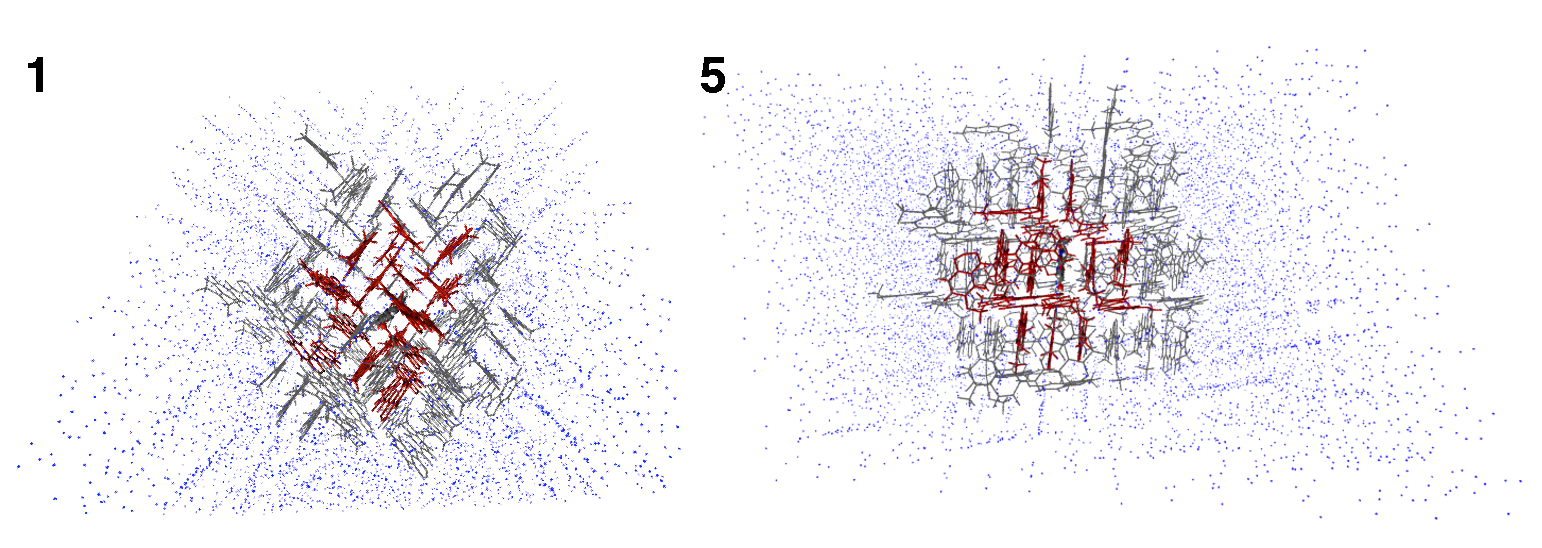
\includegraphics[width=0.9\linewidth]{4IntraInterInteractions/HC_Ewald.pdf}
  \caption[The \textbf{Ewald} charges of \textbf{M15}]{Visualisation of the \textbf{Ewald} model for compounds \textbf{1} and \textbf{5}, where the \textbf{M15} model (cyan + red + grey) is embedded in Ewald point charges, shown in blue.}
  \label{figure: HC_Ewald}
\end{figure}

\begin{figure}
\centering
  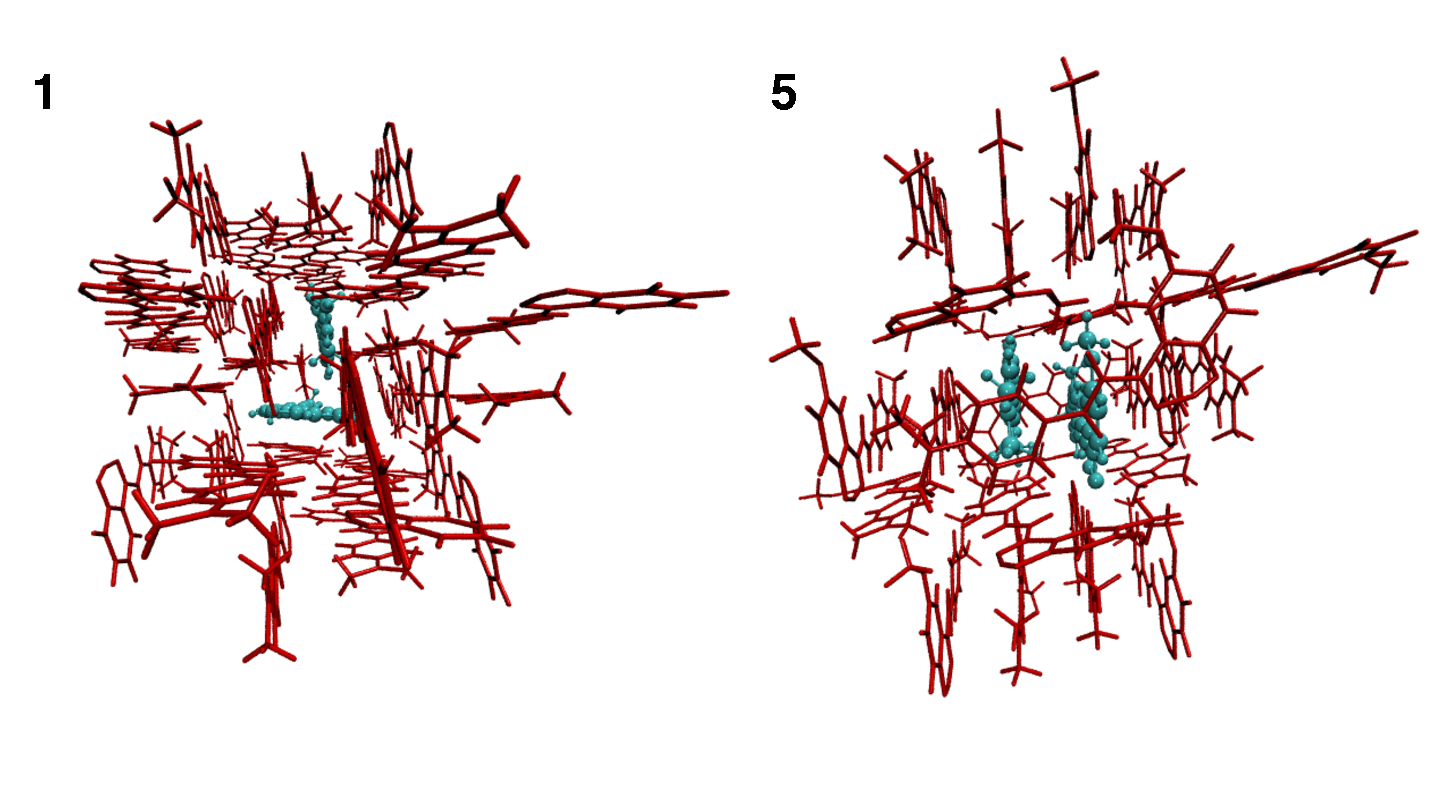
\includegraphics[width=0.9\linewidth]{4IntraInterInteractions/HC_Dimer_Models.pdf}
  \caption[The \textbf{D7} cluster models]{The \textbf{D7} model for compounds \textbf{1} and \textbf{5}. The dimer chromophore is shown in cyan, and the surrounding molecules within a radius of 7{\AA} are shown in red.}
  \label{figure: HC_Dimer_Models}
\end{figure}

ONIOM calculations were performed with the electrostatic embedding scheme. Post optimisation, single point calculations in vacuum of each ONIOM((TD-)DFT:AMBER(HF) geometry were performed to evaluate how the environment influences the energy. To assess the role of the quantum mechanical electrostatic potential during relaxation, we also perform optimisation for the \textbf{M7} and \textbf{M15} models with mechanical embedding. The nature of vertical excitations in solid state was assessed using the CALCDEN method, which classifies electronic excitations based on the electronic density localisation between donating and accepting orbitals.\cite{Crespo-Otero2012,Sen2013} 

To simulate the long-range periodic electrostatic environment experienced by the chormophore, the \textbf{M15} model was embedded in point charges derived from the Ewald method of Derenzo, Klintenberg and Weber, as described in Section \ref{section: excited_states_crystals}.\cite{Klintenberg2000,Derenzo2000} In the \textbf{Ewald} model, the chromophore was embedded in a set of point charges for each of the \szero{} and \sone{} minima and MECI geometries found with \textbf{M15} model. The initial charges were the same ESP charges used in the ONIOM models. 500 points had a fixed charge value, 1000 sample sites were used and the supercell was comprised of 4x4x4 unit cells.

The topology of the PES between the \Kstar{} minimum and the MECI was explored for the \textbf{M15} model through \ac{LIIC}, using the 6-31G(d) basis set. A relaxed geometry scan of the torsional angle $\theta$\textsubscript{tor} was also performed for the \textbf{M15} model with the 6-31G(d) basis set to probe the \ac{PES} of the \Kstar{} state. All ONIOM calculations were performed with Gaussian 09 (rev D.01).\cite{g09}

The energies at the FC state and \Kstar{} minimum for the \textbf{M15} chromophore were calculated at the RI-CC2/def2-TZVP level of theory using point charge embedding with TURBOMOLE v7.0.\cite{Hattig2002,Turbomole} The point charges were located at the atomic positions of the MM-atoms in the \textbf{M15} model.

We validate the TDDFT calculated MECI geometry of \textbf{1} and \textbf{2} in the solid state by optimising the conical intersection with the state-averaged complete active space self-consistent field  method, using an active space of 12 electrons in 11 orbitals with the 6-31G(d) basis set (SA-CASSCF(12,11)/6-31G(d)):AMBER(HF). The MECI geometry is optimised within the \textbf{M7} model with AMBER forcefield to describe the MM-level, in which all the positions of all MM atoms are frozen during the optimisation. All CASSCF calculations were performed using the MOLCAS@UU v8.0 binaries, using  the Tinker v.6.3.3 interface for the QM/MM calculations.\cite{Aquilante2016,Rackers2018} 

Intermolecular interactions are studied within Kasha's exciton framework (Section \ref{section: lom intermolecular-interactions}). The diabatization scheme of Troisi was implemented to calculate the excitonic couplings $J$ (Section \ref{section: lom exciton_couplings}).\cite{Arago2015} The dimer chromophere optimised in \szero{} in each \textbf{D7} model were extracted and single point calculations were performed of the dimer and the constituent monomers to construct the adiabatic Hamilton and the transformation matrix from the transition dipole vectors. The exciton couplings were calculate using the \texttt{exciton\textunderscore{}coupling} python package developed by myself, which has been made open-source.\cite{dommett_exciton_coupling}

The multi-model approach ensures size-consistency of the MM-region, evaluates the role of short and long-range interactions, explicitly models the long-range electrostatic potential from the crystal, and determines the role of excitonic coupling on the mechanistic interpretation.
%%%%%%%%%%%%%%
%%%%%%%%%%%%%%
\section{Results}\label{section: Inter_Results}
\subsection{Benchmarking of TDDFT}\label{section: Inter_benchmark}
Since the electronic structure method of choice in this chapter is \ac{TDDFT}, it is important to initially benchmark against the post-Hartree Fock methods used in Chapter \ref{chapter:NRdecay}. In this section we briefly compare the vertical excitations, relaxation pathways, and conical intersection geometries. Previous studies have shown that TDDFT performs well compared to CC2 for studying ESIPT.\cite{Aquino2005}

For the vertical excitations in vacuum with TD-$\omega$BX-D/6-311++G(d,p) (Table \ref{table: solid_vertical excitations}), the results of \textbf{1} and \textbf{5} compare well with CC2/def2-TZVP (Table \ref{table: HC_VEs}). The character of the first three states is the same across the  methods, with \sone{} as the bright state \pipistar{} for \textbf{1}. For compound \textbf{5}, with TDDFT \stwo{} borrows intensity from \sone{}, as with CC2 and ADC(2). The relative red shift of \textbf{5} is also similar (0.17 with CC2, 0.12 with TDDFT). It is evident that at the Franck-Condon geometry TDDFT can provide the same trends as CC2 and ADC(2), but at lower computational cost.

The excited state minima and \ac{MECI}s in the enol and keto channels were also optimised for \textbf{1}-\textbf{5} in vacuum with TD-$\omega$BX-D/6-311++G(d,p). The energies are shown in Figure \ref{figure: HC_TDDFT_Vac}. For \textbf{1} and \textbf{5}, the surfaces were also obtained at TD-$\omega$BX-D/6-31G(d) level, shown in Appendix B. The energies obtained are very similar to ADC(2) and CC2, with the keto minima at lower energy than the enol minima for \textbf{1}-\textbf{3}. As with ADC(2) and CC2, no enol minima were obtained with TDDFT, and thus the same propensity for ESIPT will be witnessed for \textbf{5}. The enol minima occur at more planar $\theta_{tor}$ angles for \textbf{1}-\textbf{3}, and therefore a larger emission energy is predicted. For \textbf{5}, similar is seen with the keto minimum, where the equilibrium geometry is more planar and thus a larger energy gap is present.

For the \ac{MECI}s in vacuum, the geometry obtained with TDDFT compare well with those obtained with CASSCF and CC2. Indeed, the TDDFT geometry is most similar to CASSCF and does not suffer from the problems of ADC(2). The \Kstar{} MECI in vacuum was calculated for \textbf{1} and \textbf{5} with the SA(2)-CASSCF(12,11)/6-31G(d). The geometries are compared to those obtained in vacuum at the {\highlevel} level of theory in Figure \ref{figure: MECI_TDDFT_vs_CASSCF_VAC}. There is an excellent agreement between the CASSCF(12,11)/6-31G(d) calculated MECI geometry (shown in cyan) and the {\highlevel} geometry (black). For compound \textbf{1}, left, the \ac{RMSD} between the two methods is 0.11 \AA. For compound \textbf{5}, the geometries are more deviated, with an RSMD of 0.59 \AA. This deviation arises due to the dihedral angle at the amino group of the molecule, which is 13{\textdegree} for TDDFT and 60{\textdegree} for CASSCF. The dihedral angles of the deprotonated phenol ring, the coordinate which drives the convergence of states, are a good match (89.9{\textdegree} for TDDFT vs 90.2{\textdegree} for CASSCF). The agreement between the TDDFT \Kstar{} conical intersection with the geometry of the CASSCF-predicted MECI in vacuum show that the protocol we employ to explore the PES with TDDFT is robust. As such the choice of TDDFT should not alter the conclusions obtained with ADC(2) and CC2. In this chapter, we also carry out single point calculations with CC2, but TDDFT is the main method chosen due to its computational efficiency and readily available implementation for QM:MM methods in ONIOM with Gaussian software. The conical intersections are also calculated using the QM:MM scheme incorporated in Molcas, using SA(2)-CASSCF(12,11)/6-31G(d):AMBER(HF) to validate the conical intersections calculated with TDDFT in ONIOM.
\begin{figure}[t]
\centering
  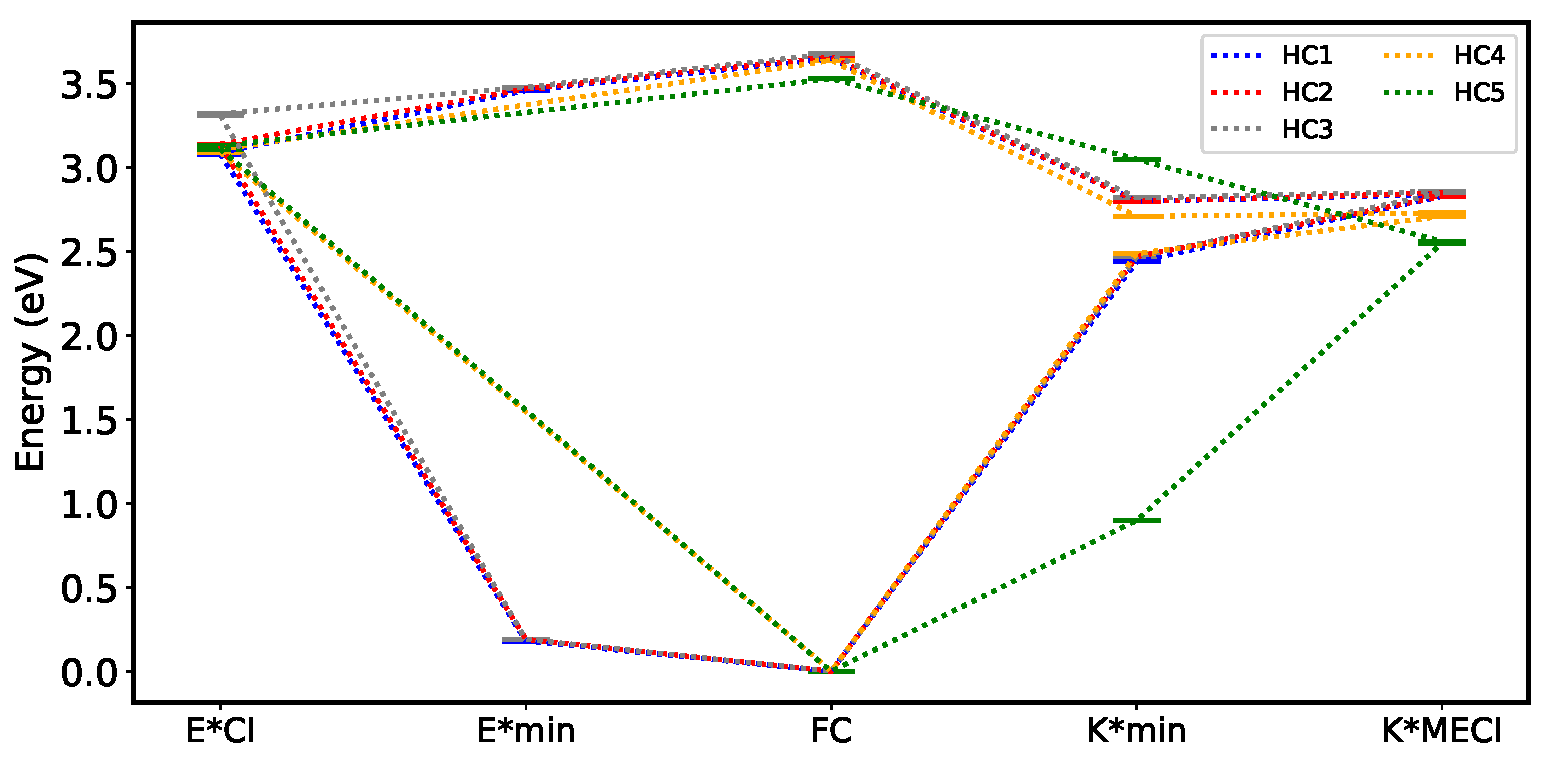
\includegraphics[width=0.8\linewidth]{4IntraInterInteractions/2HC_energies_vac_TDDFT.pdf}
  \caption[The vacuum PES of \textbf{1}-\textbf{5} with TDDFT]{The critical points on the \ac{PES} for \textbf{1}-\textbf{5} obtained at (TD-)$\omega$BX-D/6-311++G(d,p) in vacuum.}
  \label{figure: HC_TDDFT_Vac}
\end{figure}

\begin{figure}
\centering
  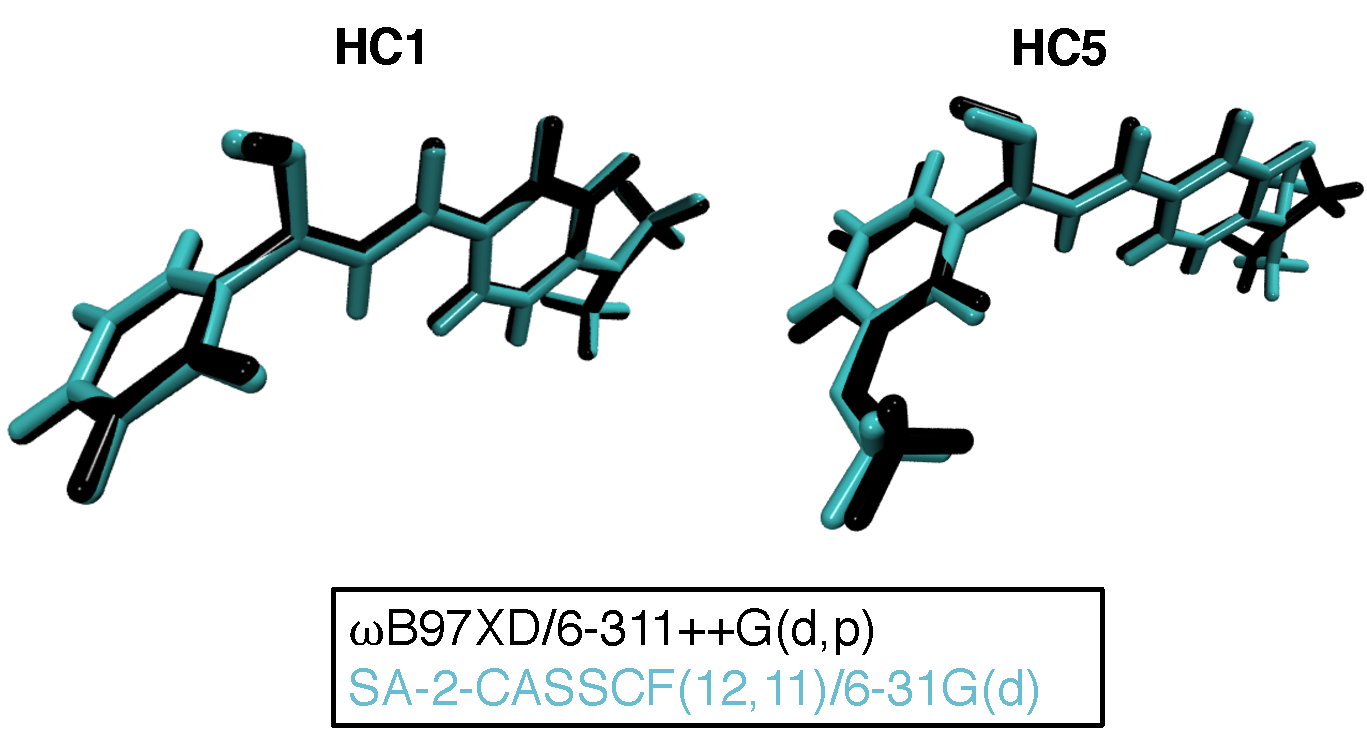
\includegraphics[width=0.75\linewidth]{4IntraInterInteractions/MECI_TDDFTvsCASSCF_VAC.pdf}
  \caption[Comparison of MECIs obtained with TDDFT and CASSCF]{Comparison of the \highlevel (black) and SA-CASSCF(12,11)/6-31G(d) (cyan) MECI geometries for compounds \textbf{1} (left) and \textbf{5} (right).}
  \label{figure: MECI_TDDFT_vs_CASSCF_VAC}
\end{figure}

\subsection{Absorption in the Molecular Crystal}\label{section: Inter_absorption}
In this section examine the absorption in the molecular crystal. For all models, the crystal environment shifts the bright state to the red with respect to absorption in vacuum. The bright state calculated for \textbf{1} with the \textbf{M} and \textbf{D} models (Table \ref{table: solid_vertical excitations}) are in very good agreement with the experimental value of 3.3 eV.\cite{Cheng2015} The bright state is calculated as 2.93 eV with RI-CC2/def2-TZVP. In the case of \textbf{5}, where no experimental absorption spectrum has been published, the energies predicted with all models are in the range of 3.4-3.5 eV. In this case the RI-CC2/def2-TZVP value of 3.33 eV aligns better with TDDFT than in \textbf{1}. There is no significant intermolecular charge transfer upon excitation in either material. 

\begin{table}
  \centering
  \caption[Excitation energies in the solid state]{Excitation energies and oscillator strengths for the first three excited singlet states of \textbf{1} and \textbf{5} in various models. Energies calculated at $\omega$B97X-D/6-311++G(d,p) level of theory and given in eV.} 
  \label{table: solid_vertical excitations}
  \begin{tabular}{lccccc}
    \hline
     & &
    \multicolumn{2}{c}{Compound \textbf{1}} 
    &
    \multicolumn{2}{c}{Compound \textbf{5}}\\
    \hline
     & & Energy (eV) & Osc.(\textit{f}) &
    Energy (eV) & Osc.(\textit{f})\\
    \hline
    
    \multirow{3}{*}{\textbf{Vacuum}} & 
	\sone{} & 3.65 & 1.143 & 3.53  & 0.870 \\
    & \stwo{} & 3.95 & 0.007 & 3.87  & 0.244 \\
    & \sthree & 4.16 & 0.002  & 3.93  & 0.013 \\
    \hdashline
   
    \multirow{3}{*}{\textbf{M7}} & 
	\sone{} & 3.20 & 1.177 & 3.42 & 0.905\\
    & \stwo{} & 4.10 & 0.001 & 3.74 & 0.236\\
    & \sthree & 4.27 & 0.030 & 4.00 & 0.002\\
    \hdashline
    
     \multirow{3}{*}{\textbf{M15}} & 
	\sone{} & 3.30 & 1.174 & 3.40 & 1.005\\
    & \stwo{} & 4.07 & 0.002 & 3.72 & 0.147\\
    & \sthree & 4.18 & 0.018 & 4.01 & 0.015\\
    \hdashline
    
    \multirow{3}{*}{\textbf{Ewald}} & 
	\sone{} & 3.30 & 1.192 & 3.50 & 0.815\\
    & \stwo{} & 4.06 & 0.002 & 3.81 & 0.320\\
    & \sthree & 4.16 & 0.015 & 3.90 & 0.008\\
    \hdashline
    
    \multirow{3}{*}{\textbf{D7-P}} & 
	\sone{} & 3.16 & 0.017 & 3.18 & 0.029\\
    & \stwo{} & 3.26 & 2.128 & 3.51 & 1.379\\
    & \sthree & 3.57 & 0.003 & 3.60 & 0.001\\
    \hdashline
    
    \multirow{3}{*}{\textbf{D7-A}} & 
	\sone{} & 3.10 & 0.061  & 3.05 & 0.000 \\
    & \stwo{} & 3.35 & 2.063 & 3.42 & 1.947 \\
    & \sthree & 3.79 & 0.006 & 3.61 & 0.012 \\
    \hline
  \end{tabular}
\end{table}
The electrostatic potential generated by the whole crystal (in the \textbf{Ewald} model) has a negligible effect for the vertical excitations of \textbf{1}, with a convergence of 3.3 eV for the bright state. In the case of \textbf{5}, a more polar structure, the effect is more significant, with a shift in the energy of around 0.1 eV. Since this is in the order of the shift associated with vibrations and does not change the nature of the excited states, even the smaller cluster models (\textbf{M7} and \textbf{D7}) can capture the main electrostatic influence on the photoexcitation.\cite{Crespo-Otero2012} However, more accurate crystalline properties would be achieved by using a more sophisticated apporach for the low-level system rather than molecular mechanics, such as QM:QM' embedding methods currently under development in the Crespo-Otero group.\cite{Rivera2018,fromage} This is particularly important for finding equilibrium structures on the excited state surface.

In going from a monomer chromophore to a dimer chromophore, the bright state shifts from \sone{} to \stwo.  For the Frank-Condon (FC) geometry, the electronic density is delocalised over both molecules in the chromophore. As a consequence of  excitonic coupling, the bright state is blue shifted in 0.06 eV and 0.15 eV  for \textbf{1} and 0.23 eV and 0.32 eV for \textbf{5} (\textbf{M7} model as reference). This is typical of H dimers within the Kasha excitonic coupling model, with oscillator strengths of \stwo{} almost double those of the monomer species in \sone.\cite{Kasha1965a} While the splitting is more significant for \textbf{5}, this does not alone explain the different properties of \textbf{1} and \textbf{5}. The role of H and J dimers in the aggregates will be investigated in the next chapter.

The largest coupling (Table \ref{table: Inter_Jcoupling}) in each compound occurs when the monomers are aligned antiparallel (\textbf{A}), of the order of 100 meV, which are in the order of those obtained for some organic semiconductors.\cite{Fornari2017} These couplings result from the favourable alignment between the nitrogen of one monomer and carbonyl group on the other monomer (approximately 4.5{\AA}). Recently, the effect of excitonic couplings on the nonradiative constants for AIE was evaluated.\citep{Li2017} For a set of five highly aromatic conjugated molecules, with \textit{J}s in the order of 10 meV, the authors found that excitonic coupling always increases the nonradiative decay constants. Based on these vibronic models, in the \Estar{} form, a larger \textit{J} on the nonradiative vibrational decay should be expected for \textbf{5}. In the next chapter, the excitonic couplings of the \textbf{HC} crystals shall be investigated in more detail.
\begin{table}
\centering
\caption[Exciton coupling in dimers of \textbf{HC1} \& \textbf{5}]{\textit{J} coupling values (eV) between units in dimers of \textbf{1} and \textbf{5} in the \textbf{D7} models}
\label{table: Inter_Jcoupling}
  \begin{tabular}{lcc}
    \hline
     & 
     {Compound \textbf{1}} &
     {Compound \textbf{5}}\\
    \hline
     & \textit{J} (eV)& 
    \textit{J} (eV)\\
    \hline
    {\textbf{D7-P}} &

    0.060 & 0.112\\
    {\textbf{D7-A}}
    & 0.105&0.150\\
    \hline
\end{tabular}
\end{table} 
%%%%%%%%%%%%%%%%%%
%%%%%%%%%%%%%%%%%%
\subsection{Radiative \textit{vs.} NonRadiative Decay}\label{section: Inter_Relaxation}
%%%%%%%%%%%%%%%%%%
%%%%%%%%%%%%%%%%%%
Relaxation to either \Estar{} or \Kstar{} minima will follow photoexcitation. The emission energies and oscillator strengths for each model are collected in Table \ref{table: Inter_emis}. In the case of \textbf{1}, significant reabsorption is expected due to the small Stokes shift for the \Estar{} minimum. This has been recently confirmed experimentally.\cite{Zahid2017} For \textbf{5}, oscillator strengths from \Estar{} are extremely small. In this context, no significant emissive response is expected from the \Estar{} state of either material. For \textbf{1}, relaxation in \Estar{} involves localisation of the electronic density on one molecule, whereas delocalisation is observed for \textbf{5}. In vacuum and the \textbf{M7}/\textbf{15} models, \Estar{} is not stable for \textbf{5}. It is stable in the dimer models due to state mixing where some of the \stwo{} character of the monomer mixes with \sone{}, such that there is less electron density lost from the phenol oxygen in \sone{}. 

\begin{table}[t]
\centering
  \caption[Emission energies in the solid state]{Emission energies and oscillator strengths from the enol and keto minima on the \sone{} PES for various models. Energies reported at \highlevel level of theory and given in eV.}
\label{table: Inter_emis}
  \begin{tabular}{lcccc}
    \hline
    &
    \multicolumn{2}{c}{Compound \textbf{1}} 
    &
    \multicolumn{2}{c}{Compound \textbf{5}}\\
    \hline
     & \Estar{} (\textit{f}) & \Kstar{} (\textit{f}) &
    \Estar{} (\textit{f}) & \Kstar{} (\textit{f})\\
    \hline
    
    {\textbf{M7}} & 
	3.03 (1.207) & 2.67 (1.191) & -  & 2.15 (0.461) \\

    {\textbf{M15}} & 
	3.10 (1.225) & 2.61(0.977) & - & 2.17 (0.490)\\
    
    {\textbf{Ewald}} & 
	3.12 (1.214) & 2.66 (1.052) & -  & 2.18 (0.486)\\

    {\textbf{D7-P}} & 
	3.01 (0.479) & 2.56 (0.725) & 2.45 (0.002) & 2.15 (0.312) \\
    
    {\textbf{D7-A}} & 
	2.96 (0.119) & 2.59 (0.616) & 2.81 (0.000)  & 2.32 (0.388) \\
	\hline
  \end{tabular}
\end{table}

Geometries of the \Estar{} and \Kstar{} minima are planar in the solid state. Since no double proton transfer \Kstar{} minimum was found for \textbf{1},  emission is expected from a localised \Kstar{} state. The experimental emission spectrum for \textbf{1} can be assigned to the \Kstar{} state ranging from 1.5-2.1 eV. The predicted values are blue shifted to 2.7 eV (CC2/def2-TZVP predicts emission at 2.2 eV). The flatness of the \sone{} surface with respect to the dihedral angle suggests that emission from a range of geometries is possible. To investigate this, a relaxed geometry scan was performed at \lowlevel:AMBER(HF) for both \textbf{1} and \textbf{5}, where $\theta_{tor}$ was incrementally increased in the \textbf{M15} model and frozen during relaxation, shown in Figure \ref{figure: HC_Oniom_Scan}. Between 0 and 40{\textdegree}, the \sone{} surface is quite flat, whilst the energy gap between \sone{} and \szero{} states ranges from 2.7 eV (\textit{f}=0.973) to 2.2 eV (\textit{f}=0.496). The flatness of the surface, and the high oscillator strengths along the coordinate, suggest that emission from a range of dihedral angles less than 40{\textdegree} is possible, in particular since dihedral rotation energetically favourable relaxation pathway in vacuum. Also important to take into account when considering the emission energies are the limitations of the QM:MM method. All of the exterior atoms are frozen and treated at MM level, without the possibility of any mutual polarisation between the regions. As such, the environment cannot respond to the changes in electronic density of the chromophore, which can be rather large in the case of ESIPT systems. As such, the additional relaxation from mutual charge polarisation is not present here, and the emission energies are somewhat overestimated. The dimer models partially alleviate this by having a polarisable molecular counterpart, and the emission energy is reduced. 

\begin{figure}[t]
\centering
  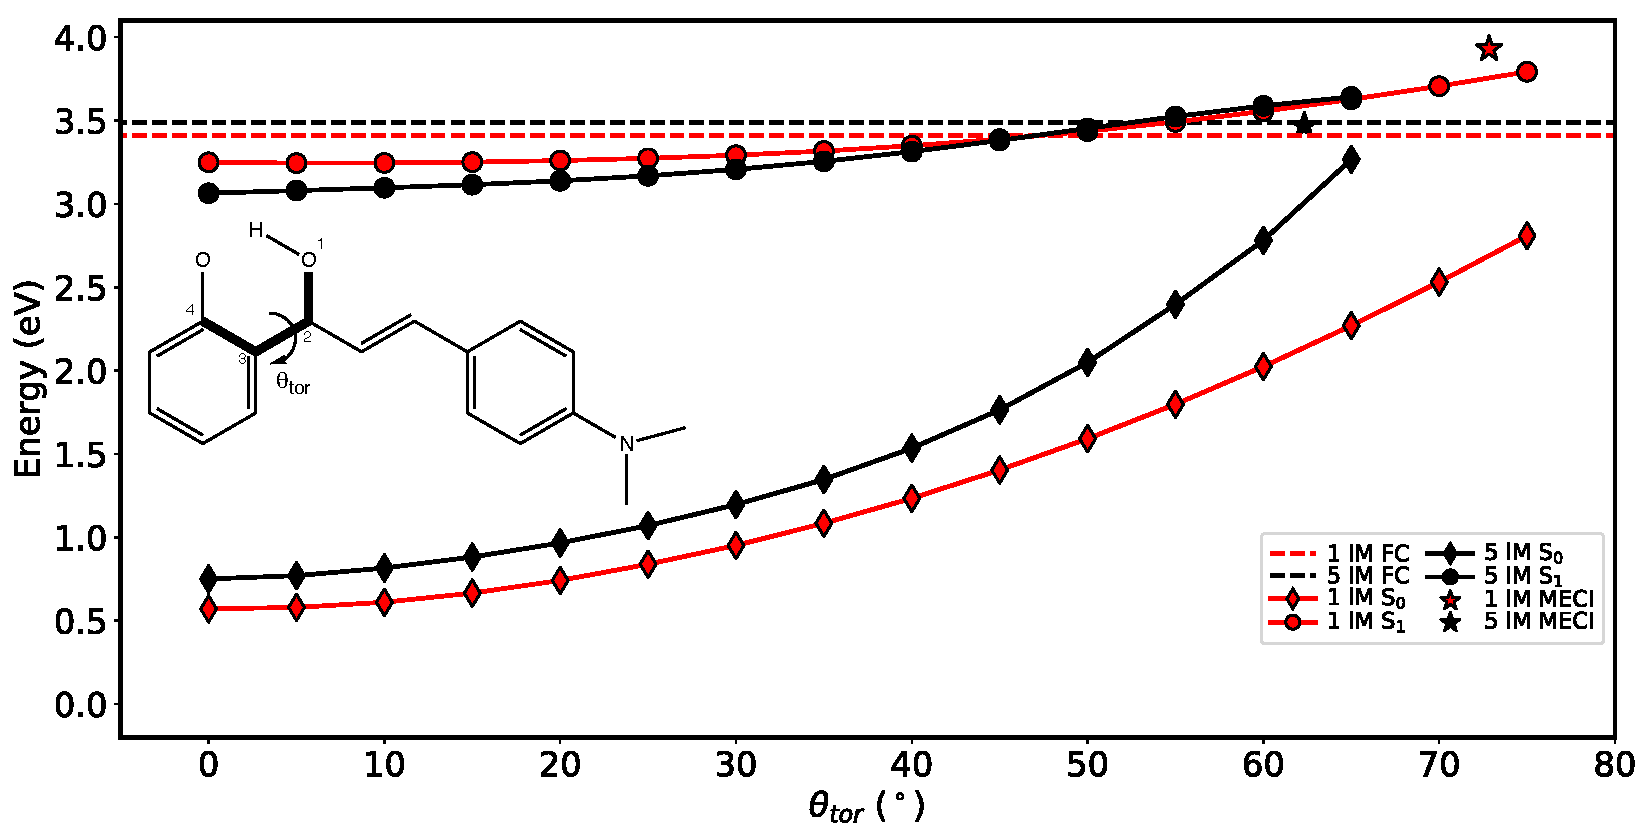
\includegraphics[width=0.8\linewidth]{4IntraInterInteractions/HC_Oniom_Scan.pdf}
  \caption[Relaxed geometry scan in the crystal]{Relaxed geometry scan of the dihedral angle $\theta_{tor}$ calculated at ONIOM($\omega$B97X-D/6-31G(d)):AMBER level of theory for compounds \textbf{1} (red) and \textbf{5} (black) in the \textbf{M15} model. Also plotted are the bright excitation energies (dashed lines) and the MECI energy (stars) for both compounds in the \textbf{M15} model.}
  \label{figure: HC_Oniom_Scan}
\end{figure}

In \textbf{5}, there  exists a double-\Kstar{} state, where both monomers undergo ESIPT. This state is nonemissive in \sone{} (\textit{f}=0.002) lying 0.5 eV above the bright FC state. The localised single proton transfer state in \textbf{5} has emission in the range 2.2-2.3 eV (1.7 eV with CC2). Oscillator strengths, though half the value of the obtained for \textbf{1}, are still significant (0.312 and 0.388). Therefore, while emission from \textbf{1} should be brighter than from \textbf{5}, radiative mechanisms alone cannot explain the negligible quantum yield of \textbf{5}. The structural similarity of the \Estar{} and \Kstar{} minima, namely that the \Estar{} state is planar, means that the pathways no longer compete in the excited state. The bifurcation seen in vacuum is not expected to exist in the solid state, and relaxation to \Kstar{} can follow relaxation in \Estar{}. To maximise the quantum yield, efficient population transfer \Kstar{} is important, since little emissive response will be witnessed from \Estar{} due to the small Stokes shift.

The location of the nearest CI to the \Estar{} and \Kstar{} minima can help understand the balance between radiative and nonradiative decay. In Chapter \ref{chapter:NRdecay}, we saw that in vacuum both pathways lead to energetically accessible conical intersections \textit{via} intramolecular rotation. In the solid, intramolecular rotation in \Estar{} is completely blocked and the \Estar{} CI is accessed instead \textit{via} a stretch of the bridging unsaturated bond. This is associated with an energy cost of upward of 5 eV from the FC \sone{} energy for both crystals. Consequently, molecular aggregation completely blocks the \Estar{} nonradiative decay pathway in both \textbf{1} and \textbf{5}. For \textbf{1}, the \sone/\szero{} MECI associated with the \Kstar{} state lies 0.5-1.0 eV above the \sone{} energy for the FC geometry (Figure \ref{figure: Solid_Mechanism_D7}). For \textbf{5}, the \sone/\szero{} MECI is classically accessible with a barrier of 0.4 eV from the \Kstar{} minimum. While less favourable than in gas phase (barrier 0.2 eV), the system has enough energy to access the conical intersection. Therefore, in compound \textbf{5} the excited state population can decay nonradiatively through the MECI and back to the ground state, whereas in \textbf{1} the population remains in the \Kstar{} state until fluorescence.

\ac{LIIC} between the \Kstar{} minimum and MECI  show the existance of a barrier of 1.4 eV (w.r.t to FC \sone{}) to reach the MECI for \textbf{1} compared to 0.14 for compound \textbf{5} (Figure \ref{figure: solid_liic}. It is important to state that the LIIC barriers represent an upper bound for barriers on the PES and the true barriers will be smaller, since coordinated relaxation was neglected at each step. However, the barriers here offer further evidence that the MECI of \textbf{1} is inaccessible and \textbf{5} is not. 

\begin{figure}[t]
\centering
  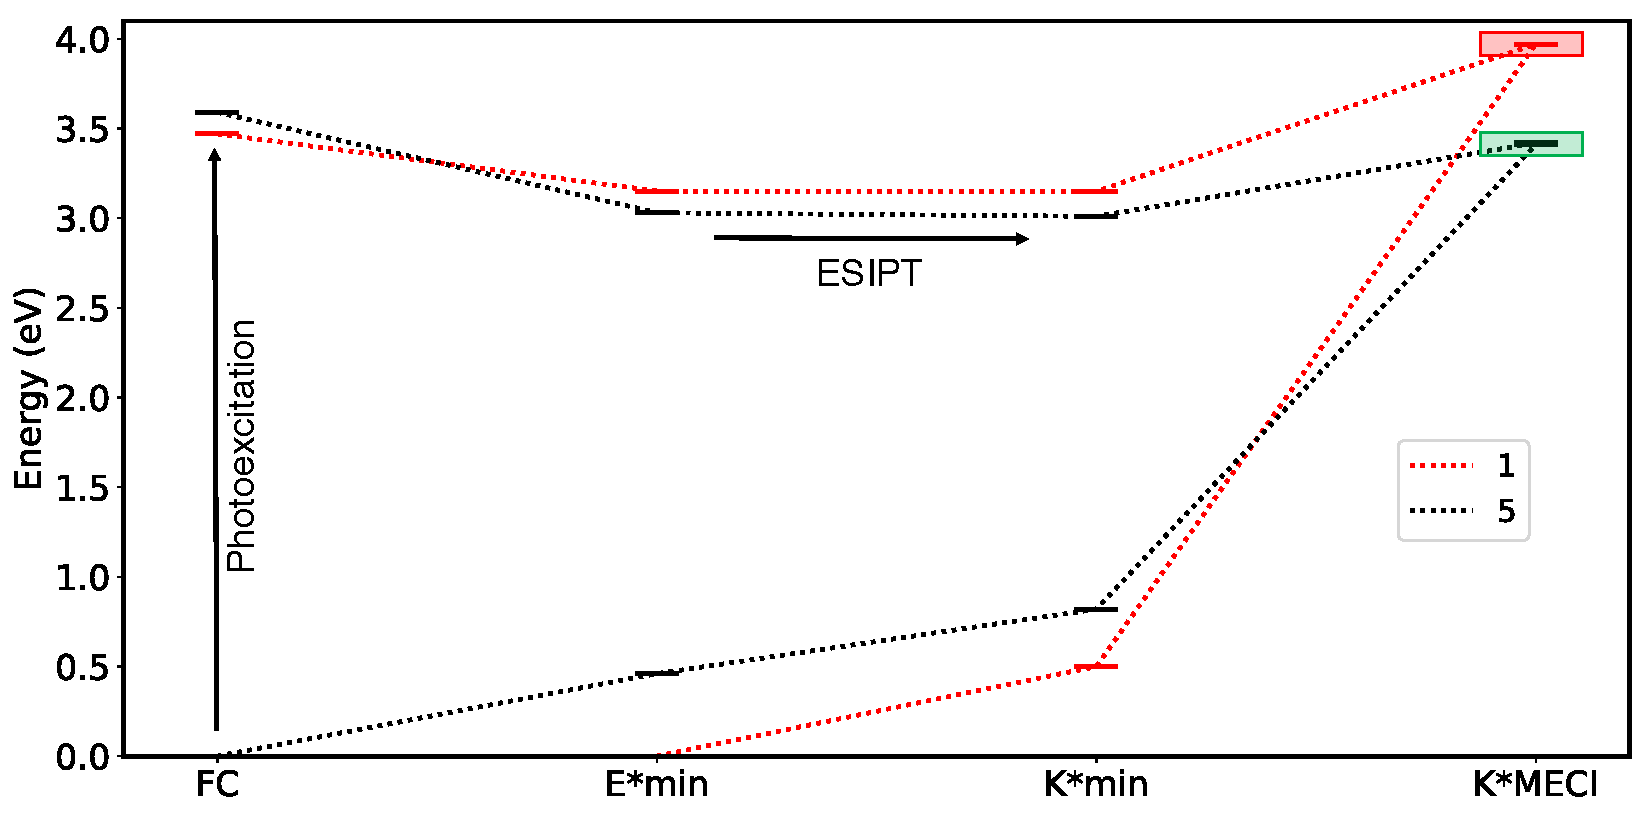
\includegraphics[width=0.8\linewidth]{4IntraInterInteractions/D7.pdf}
  \caption[Decay mechanism in the molecular crystal in \textbf{D7} model]{Energy of the \szero{} and \sone{} states at the  Franck-Condon (FC) point, \Estar{} and \Kstar{} minima, and the MECI of \textbf{1} and \textbf{5} with the \textbf{D7} model with ONIOM($\omega$B7X-D/6-31G(d)):AMBER level of theory. The accessibility is colour coded.}
  \label{figure: Solid_Mechanism_D7}
\end{figure}

\begin{figure}[t]
\centering
  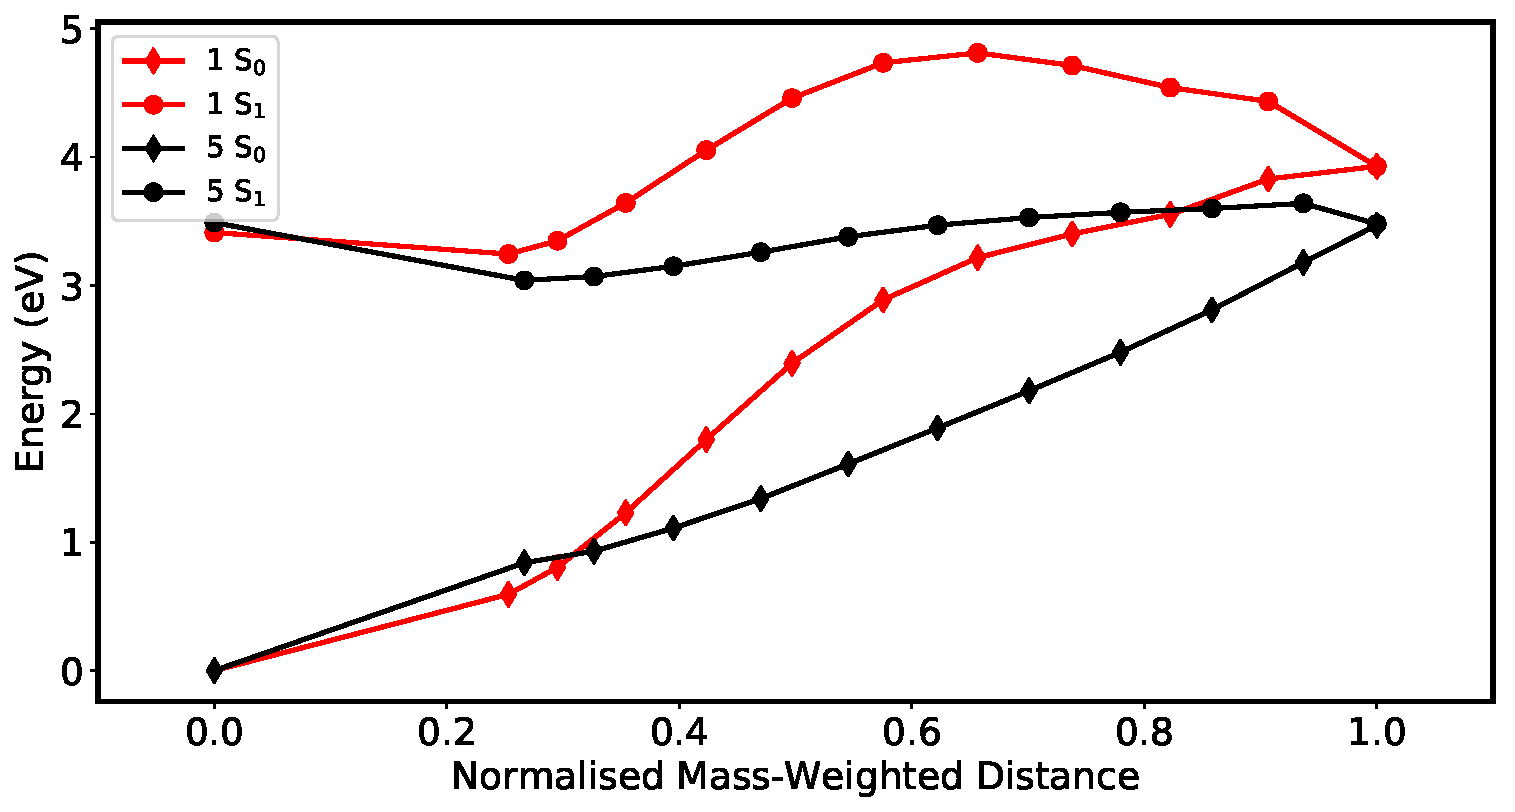
\includegraphics[width=0.8\linewidth]{4IntraInterInteractions/ONIOM_LIIC.pdf}
  \caption[Linear interpolation of internal coordinates in the solid state]{Linear interpolation of internal coordinates between the Franck Condon state, the \sone{} minimum, and the MECI for \textbf{1} and \textbf{5}.}
  \label{figure: solid_liic}
\end{figure}

\begin{table}
\caption[Relative energies with and without electrostatic embedding in monomer models]{Relative energies for the FC, \Estar{} and \Kstar{} minima, and MECI on the PES for \textbf{1} and \textbf{5} for the \textbf{M7} and \textbf{M15} models, with ME and EE during the optimisation. All values presented in eV relative to the corresponding ground state and are calculated at ONIOM($\omega$B97X-D/6-31G(d)):AMBER level of theory. The oscillator strength \textit{f} is also given.}
\label{table: ONIOM_comparison}
\centering
\begin{tabular}{ccccccccccc} 
\hline
\multicolumn{11}{c}{ Mechanical Embedding (ME) } \\
\hline
&  & \multicolumn{4}{c}{ Compound \textbf{1} } & & \multicolumn{4}{c}{ Compound \textbf{5} } \\
\hline
\multicolumn{2}{c}{} & FC & \Estar{}min & \Kstar{}min & MECI & & FC & \Estar{}min & \Kstar{}min & MECI \\
\hline
\multirow{3}{*}{ \textbf{M15} } & 
S$_{0}$& 0.00 & 0.18 & 0.82 & 4.02 & & 0.00 & - & 0.82 & 3.71 \\ 
& S$_{1}$& 3.74 & 3.56 & 3.32 & 4.03 & & 3.60 & - & 3.07 & 3.71 \\
& \textit{f}& 1.150 & 1.207 & 0.503& - & & 0.749&- &0.475& - \\
\hdashline
\multirow{3}{*}{ \textbf{M7} } & S$_{0}$ & 0.00 & 0.18 & 0.84 & 3.93 & & 0.00 & - & 0.80 & 4.05 \\
& S$_{1}$ & 3.73 & 3.56 & 3.32 & 3.93 & & 3.60 & - & 3.06 & 4.06 \\
& \textit{f}  & 1.511 &1.204 &0.563  & - & & 0.744&- &0.484&-\\

\hline
\multicolumn{11}{c}{ Electrostatic Embedding (EE) } \\
\hline
&  & \multicolumn{4}{c}{ Compound \textbf{1} } & & \multicolumn{4}{c}{ Compound \textbf{5} } \\
\hline
\multicolumn{2}{c}{} & FC & \Estar{}min & \Kstar{}min & MECI & & FC & \Estar{}min & \Kstar{}min & MECI \\
\hline
\multirow{3}{*}{ \textbf{M15} } & S$_{0}$ & 0.00 & 0.10 & 0.59 & 3.93 & & 0.00 & - & 0.84 & 3.47 \\
& S$_{1}$ & 3.41 & 3.31 & 3.25 & 3.93 & & 3.49 & - & 3.04 & 3.48 \\
& \textit{f} & 1.202 & 1.253 &0.928 &- & &0.926&-&0.487&- \\
\hdashline
\multirow{3}{*}{ \textbf{M7} } & S$_{0}$ & 0.00 & 0.08 & 0.48 & 4.04 &  & 0.00 & - & 0.88 & 3.48 \\
& S$_{0}$ & 3.32 & 3.23 & 3.20 & 4.05 & & 3.50 & - & 3.05 & 3.49 \\
& \textit{f} &  0.664 & 1.232 & 1.146 & -& &0.815 &-&0.459&-\\
\hline
\end{tabular}
\end{table}

To further explore the electrostatic effect, the critical points of the \ac{PES} were reoptimised without electrostatic embedding for the monomer models. The energies in comparison to those obtained with electrostatic embedding are given in Table \ref{table: ONIOM_comparison}. Crucially, the accessibility of the MECI depends on its stabilisation with respect to the initially populated excited states. For compound \textbf{1}, the electrostatic potential stabilises the \sone{} state at the FC region but has a smaller effect on the energy of the MECI. Both of these factors decrease the accessibility of the nonradiative channel. A similar effect is seen for both the \textbf{M7} and \textbf{M15} models, suggesting that these are short to medium range effects and are not as a result of long- range Coulombic interactions. For \textbf{5}, the stabilisation of the MECI is larger than for the \sone{} state. Therefore the accessibility of the MECI in \textbf{5} is aided by the short-range electrostatic interactions with the surrounding molecules when treated at QM-level. 

Moreover, within the mechanical embedding approach, the MECI geometries are similar, but both MECI have energies lying above the photopopulated state for \textbf{5} and below for \textbf{1}. This indicates that steric hindrance in the crystal determines level of distortion of the MECIs, but a quantum-mechanical treatment of Coulombic interactions modulate their total energies. The same conclusions can be drawn from the monomer models, for which the energy levels of \textbf{M15} are shown in Appendix C. As mentioned above, there is  no \Estar{} minimum located for \textbf{5}. As such, it is expected that the short range interactions present in the dimer chromophore restrict torsional relaxation, whilst long range electrostatic interactions, imperfectly included in these models due to the lack of self-consistent polarisation, can help stabilise the excited state, particularly when the geometry of the chromophore most resembles the exterior charge distrubtion, as at absorption.

\begin{figure}
\centering
  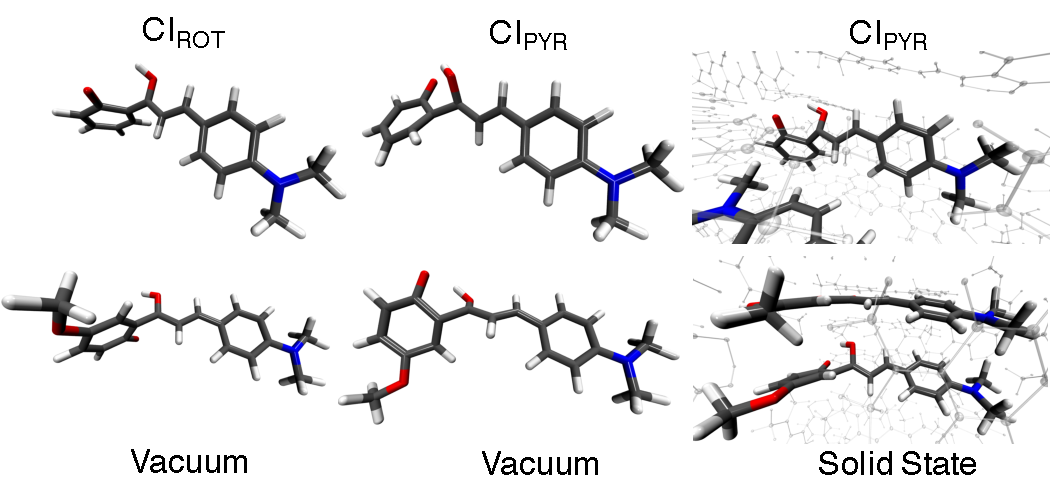
\includegraphics[width=0.8\linewidth]{4IntraInterInteractions/HC_1_5_conicals.pdf}
  \caption[Comparison of vacuum and solid state conical intersections]{Geometry of the \Kstar{} MECI in vacuum (left and center) and in the solid state (right) for \textbf{1} (top) and \textbf{5} (bottom).}
  \label{figure: HC_1_5_conicals}
\end{figure}

The \Kstar{} MECI is accessed \textit{via} a combination of intramolecular rotation (ROT) and carbonyl pyramidalisation (PYR), with a puckering of the deprotonated phenol ring (Figure \ref{figure: HC_1_5_conicals}). In contrast with the most stable conical intersections (CI\textsubscript{ROT}) in vacuum, the MECI structures in the solid state (CI\textsubscript{PYR}) display a significant pyramidalisation of the carbonyl carbon, with a puckering angle of 41\textdegree{}. The puckering angle is defined as the angle between the the (protonated) carbonyl and plane made by the $\alpha$ carbons. The pyramidalisation is at the expense of $\theta_{tor}$, which decreases with respect to the vacuum MECI.  This is caused by the steric restrictions of the surrounding molecules, meaning CI\textsubscript{ROT} can no longer be accessed and the pyramidalised conical intersection becomes the MECI. For \textbf{5}, the \Kstar{} MECI has similar geometric parameters as \textbf{1}, but with a smaller pyramidalisation of the carbonyl group (21\textdegree{}). Interestingly, a similar CI\textsubscript{PYR} conical intersection can be found in vacuum for both compounds, (Figure \ref{figure: HC_1_5_conicals}), with the CI\textsubscript{PYR} lying 0.9 eV above the CI\textsubscript{ROT} for \textbf{1} and 0.6 eV for \textbf{5}. Therefore, the crystal changes the order stability of the conical intersection manifold, stabilising CI\textsubscript{PYR} over CI\textsubscript{ROT} compared to in vacuum. In vacuum, CI\textsubscript{PYR} is energetically accessible in both \textbf{1} and \textbf{5}, lying 0.04 below the \sone{} state for \textbf{1}. For \textbf{5}, CI\textsubscript{PYR} lies 0.33 eV below the initial excitation energy in vacuum. CI\textsubscript{ROT} in vacuum is also accessed at lower rotational distortion and lower energy than the corresponding CI for \textbf{1}. As such, since the accessibility of the conical intersection for \textbf{5} is witnessed in vacuum, the larger stability of the MECI in the solid state compared to \textbf{1} is mainly explained by the electronic effects provided by the methoxy substituent, aided by the electrostatic potential discussed above. As a result, \textbf{5} has enough energy to deactivate through the conical intersection and return to the ground state via the nonradiative pathway, a channel infeasible for compound \textbf{1}. 

\begin{table}
  \centering
  \caption[Comparison of MECI angle parameters]{Comparison of MECI angle parameters for \textbf{1} and \textbf{5} in vacuum and the solid state} 
  \label{table: conical_parameters}
  \begin{tabular}{lccccc}
  \hline
  & \multicolumn{2}{c}{Compound \textbf{1}} & \multicolumn{2}{c}{Compound \textbf{5}}\\
  \hline
  & $\theta_{puck}$ & $\theta_{tor}$ & $\theta_{puck}$ & $\theta_{tor}$ \\
  \hline
  Vacuum CI\textsubscript{ROT} & 8\textdegree{} & 89\textdegree{} & 5\textdegree{} & 90\textdegree{}\\
  Vacuum CI\textsubscript{PYR} & 65\textdegree{} & 36\textdegree{} & 62\textdegree{} & 27\textdegree{}\\
  Solid (\textbf{sD}) CI\textsubscript{ROT} & 65\textdegree{} & 41\textdegree{} & 67\textdegree{}&21\textdegree{}\\
  \hline
  \end{tabular}
\end{table}

\section{Summary and Conclusions}\label{section: Inter_conclusions}

In summary, the analysis of two materials with contrasting emissive properties illustrates how the balance of intermolecular and intramolecular factors can control the radiative and nonradiative mechanisms underlying their light response. The relaxation mechanisms for \textbf{1} and \textbf{5} shown in Figures \ref{figure: HC_1_Density_Mechanism} and \ref{figure: HC_5_Density_Mechanism}. After initial photoabsorption the excited state is delocalised in the enol form, where $\pi$-$\pi$ interactions in \textbf{5} increase the excitonic coupling, which plays a role at the Franck-Condon state where absorption is delocalised. In the next chapter, the delocalisation of the exciton in the enol channel shall be scrutinised. The systems relax in \Estar{}, where a minimum exists on the PES and emission with very small Stokes shift is possible, but self-absorption would most likely be witnessed. Nonradiative decay through a conical intersection in the enol channel is unlikely due to its high energy. 

Alternatively, localisation allows ESIPT, followed by relaxation. For \textbf{1}, the nearest MECI in the \Kstar{} channel is classically inaccessible and so fluorescence is witnessed. For \textbf{5}, the MECI is lower in energy, due to the difference in electronic density distribution in \sone{} on account of the methoxy group, and the wavepacket can funnel nonradiatively to \szero{}. For the \Kstar{} channel, the crystal changes the relative energy of two conical intersections present in gas phase, stabilising a structure where the carbonyl group pyramidalises. The calculations show that either nonradiative delocalised transport processes (\Estar{} channel) or localised deactivation through the ESIPT (\Kstar{} channel) are more likely in \textbf{5} than in \textbf{1}. The interplay of all discussed factors results in an enhance emissive response of \textbf{1} and no fluorescence in \textbf{5} in the solid state. 

\begin{figure}
  \centering
  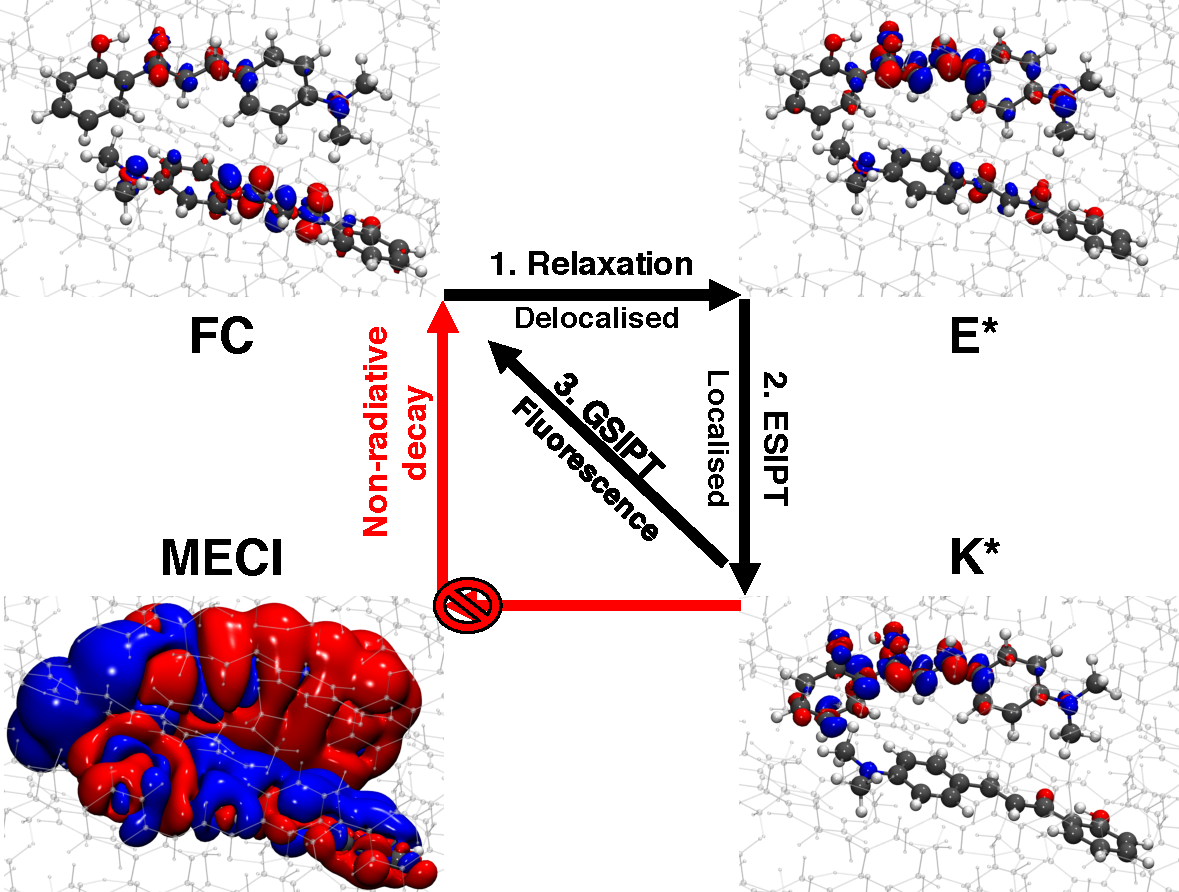
\includegraphics[width=0.8\linewidth]{4IntraInterInteractions/HC_1_Density_Mechanism.pdf}
  \caption[Radiative decay in \textbf{HC1}]{The mechanism for nonradiative decay in compound \textbf{2}. Also shown are \sone-\szero{} electron density differences (red: \sone{}, blue: \szero{}).}
  \label{figure: HC_1_Density_Mechanism}
\end{figure}

\begin{figure}
  \centering
  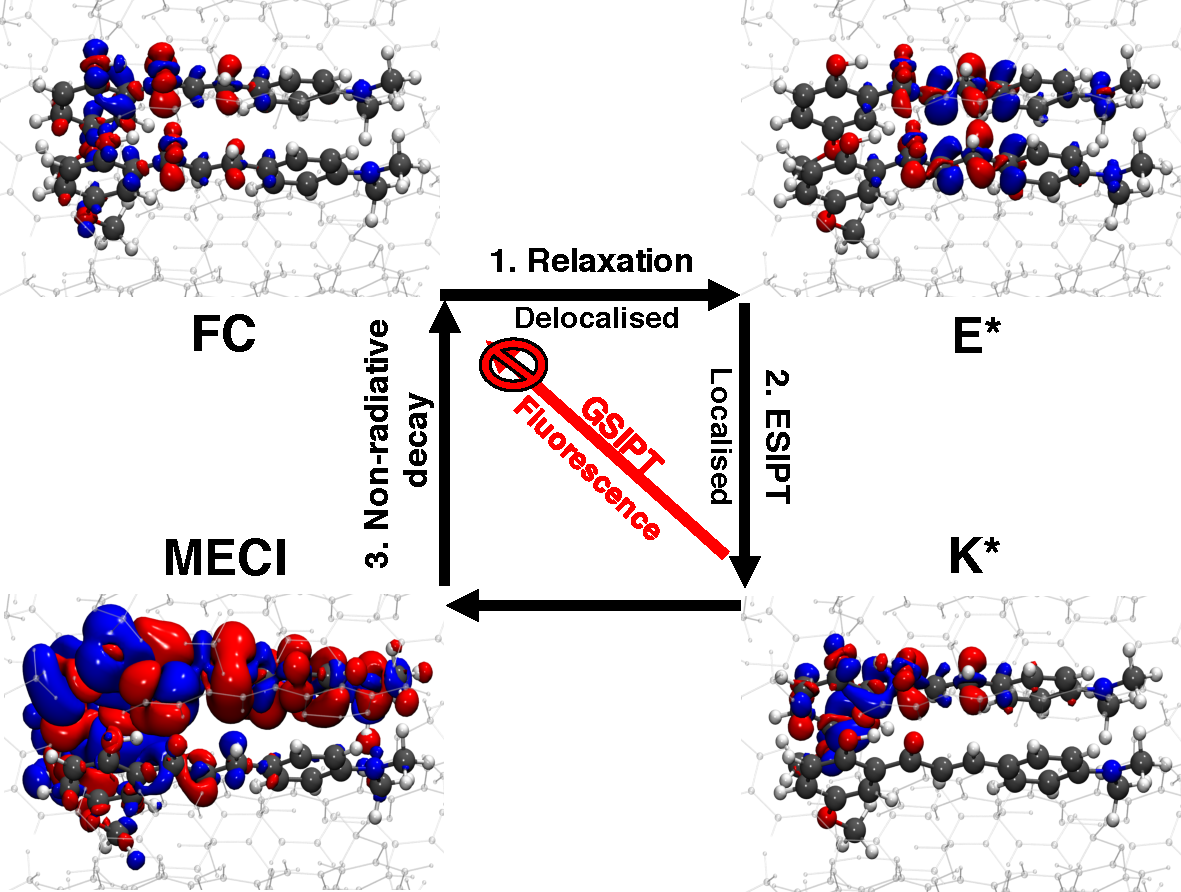
\includegraphics[width=0.8\linewidth]{4IntraInterInteractions/HC_5_Density_Mechanism.pdf}
  \caption[Nonradiative decay in \textbf{HC5}]{The mechanism for nonradiative decay in compound \textbf{5}. Also shown are \sone-\szero{} electron density differences (red: \sone{}, blue: \szero{}).}
  \label{figure: HC_5_Density_Mechanism}
\end{figure}

From these results, some design principles can be proposed for more efficient solid-state emitters. As strong electrostatic interactions aid the deactivation through nonradiative pathways, it is clear why many of the reported AIE fluorophores are nonpolar. For the ESPIT chromophores, stabilising \Estar{} over \Kstar{} minima could be favourable because the \Estar{} nonradiative pathway through a conical intersection is hampered in the solid state. For this, the nature of the \Estar{} state must be altered to induce a larger Stokes shift. Alternatively, if the \Estar{} state is made more unstable by increasing the lability of the transferring proton, the population transfer to the \Kstar{} channel will increase. To maximise returns, access to the pyramidal \Kstar{} MECI can be further hindered by imposing geometrical restrictions, such as introducing fused rings to the molecular structure. Other studies in ESIPT systems have shown that torsional restraint can also be achieved by coordination to metals.\cite{Karsili2016} For the \Kstar{} channel, efficient localisation of excited state to one monomer, bias for \Kstar{} over \Estar{} decay and an energetically inaccessible conical intersection are all highly desirable. Indeed path agnosticity for compound \textbf{1}, which is evenly distributed for \Estar{} and \Kstar{}, may prevent efficient transfer to the emissive \Kstar{} state. This is remedied in \textbf{5} by the bias for ESIPT but the low-lying MECI prevents fluorescence. The design of a chromophore to combine the \Kstar{} bias of \textbf{5} with the stability of \textbf{1} would surely be a promising candidate for a highly efficient fluorophore.  In the next chapter a new class of AIE system based on the \textbf{HC} family shall be introduced and investigated, building on the conclusions of Chapters \ref{chapter:NRdecay} and \ref{chapter: Inter} for fluorophore design. 
\chapter[Connecting Chromophore Design with Crystal Morphology]{Connecting Chromophore Design with\\ Crystal Morphology}
\label{chapter: Connecting}
\begin{figure}[H]
\centering
  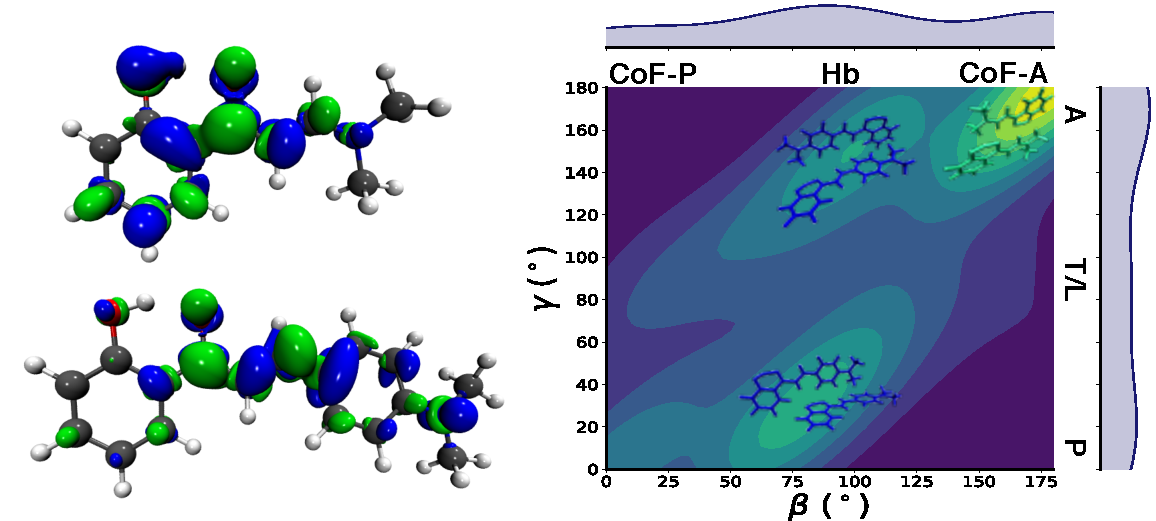
\includegraphics[width=0.7\linewidth]{5ConnectingCrystalStructure/3toc.pdf}
\end{figure}
\section{Introduction}\label{section: Connecting_Introduction}

In Chapters \ref{chapter:NRdecay} and \ref{chapter: Inter} the \acp{PES} of a range of \ac{HC} derivatives were mapped, first in vacuum and then crystalline form. Through the topology of the \acp{PES} and the associated energy differences between states, we elucidated the AIE mechanism of \textbf{HC1} and the nonemission of \textbf{HC5}. In doing so, we isolated three key design principles to increase the quantum yield of fluorescence for ESIPT chromophores in the solid state:
\begin{enumerate}
    \item bias for \Kstar{} decay over \Estar{}
    \item localisation of excited state to one monomer 
    \item an energetically inaccessible conical intersection
\end{enumerate}

In this Chapter the scope of the study is extended as these design rules are applied to a new set of ESIPT systems. To the test set we add two fluorine-substituted \ac{HC} derivatives, \ac{HC}\textbf{6} and \textbf{HC7}.\cite{Cheng2016} Additionally, four completely new compounds with lasing properties are considered. Closely related to \acp{HC} are the family of \ac{HP} derivatives.\cite{Tang2016} In contrast to \acp{HC}, and other organic fluorophores, \ac{HP} compounds contain only a single aryl group and have remarkable \ac{QE}, ranging from 0.72-0.84. This has been qualitatively attributed experimentally to the herringbone packing mode and molecular rigidity reducing nonradiative decay. The increased quantum yield of the \acp{HP}, with respect to the \acp{HC}, make them prime candidates to test the efficacy of our  design rules. The eleven compounds studied in this Chapter are summarised in Table \ref{table: chalcones} and shown in Figure \ref{figure: HCHP_structures}.
\begin{figure}[t]
\centering
  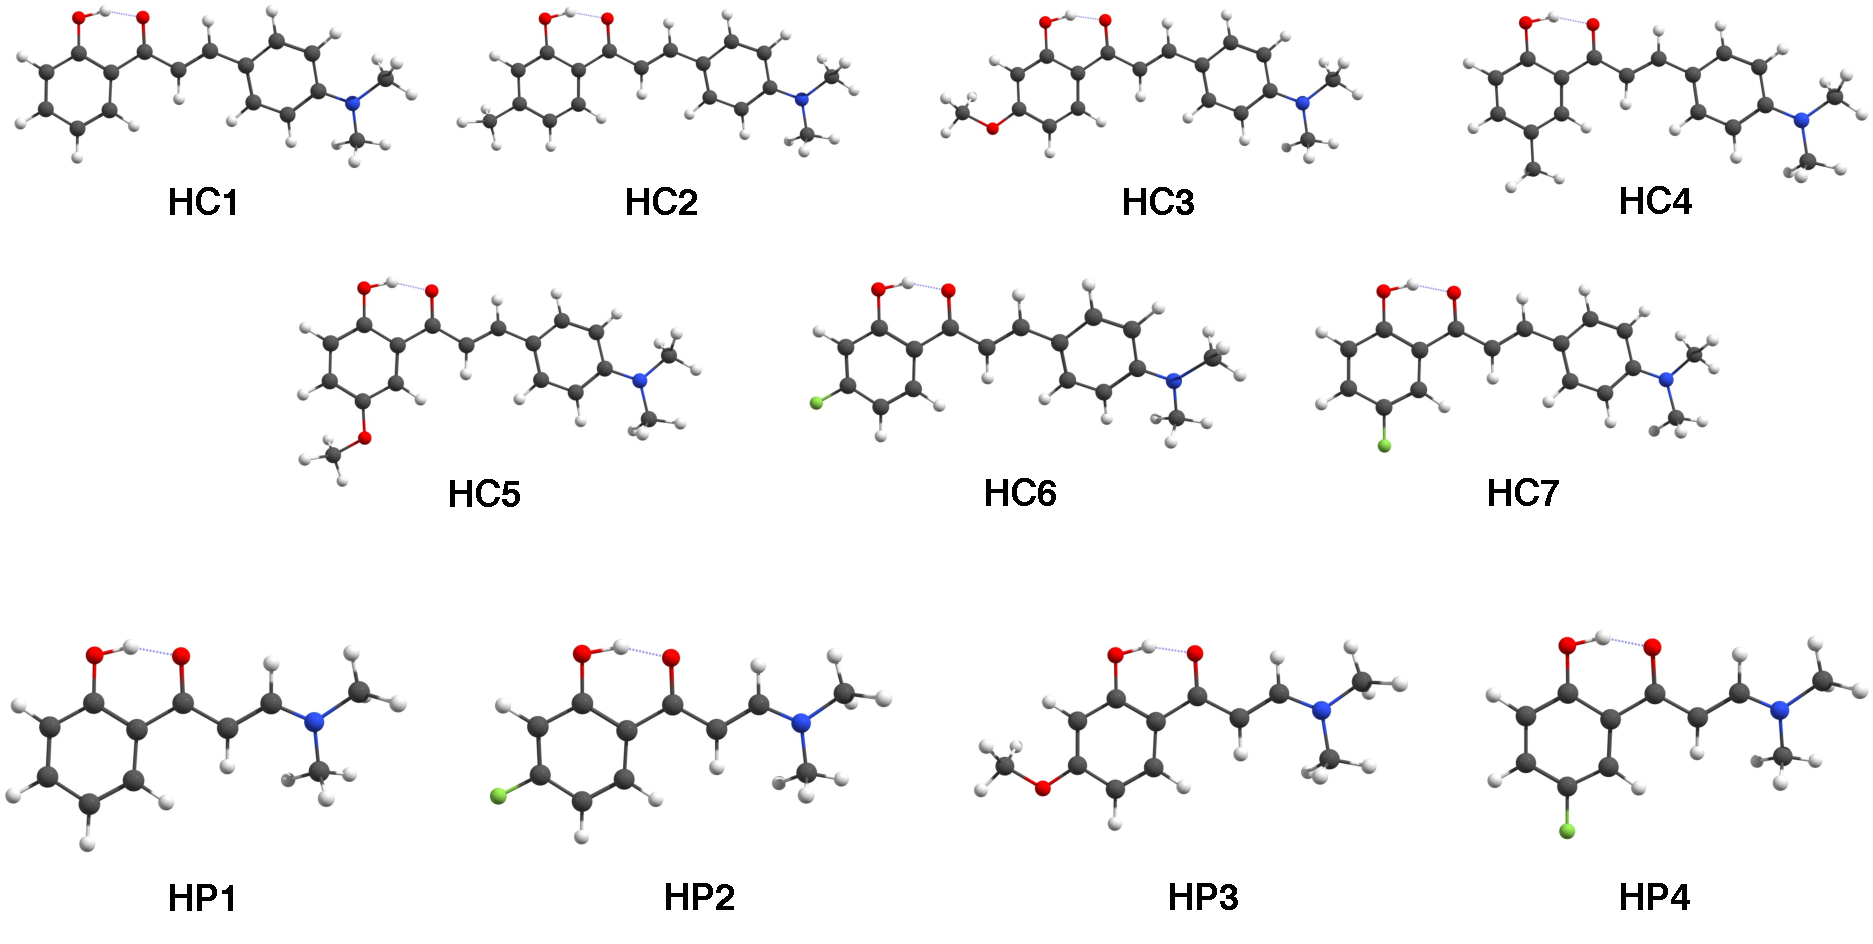
\includegraphics[width=\linewidth]{5ConnectingCrystalStructure/HCHP_structures.pdf}
  \caption[Molecular structures of eleven \textbf{HC} and \textbf{HP} compounds]{The molecular structure of the seven \textbf{HC} and four \textbf{HP} compounds under investigation.}
  \label{figure: HCHP_structures}
\end{figure}
Herein we investigate the factors which mediate the increased fluorescence activity for \textbf{HP} compared to \textbf{HC} systems. In the following sections we address molecular and material properties of the eleven compounds to investigate why the \acp{HP} systems have an increased \ac{QE} compared to their \textbf{HC} counterparts. We will show how a combination of electronic properties and crystal packing give the \textbf{HP} systems an increased potency for each of the three design rules, resulting in increased fluorescence in the solid state. Particular focus will be given to \textbf{HC1}, \textbf{HC5}, and \textbf{HP1}, which will act as exemplar systems due to their differing fluorescence behaviour.

After outlining the computational methods used, we address the molecular properties of the \textbf{HC} systems. We map the \acp{PES} of \textbf{HP1}-\textbf{4} in vacuum, to locate the nonradiative decay channels and gauge the substituent effects, showing how the increased bias for the keto channel promotes \ac{ESIPT} in these systems, fulfilling design rule one. We then move to the crystalline state and show how a stable \Kstar{} minimum and inaccessible conical intersection promote radiative decay in \textbf{HP1}, satisfying design rule three. We compute the radiative decay rates for \textbf{HC1}, \textbf{HC5}, and \textbf{HP1} \textit{via} two methods to compare the exemplar compounds, and examine the Huang-Rhys factors to qualitatively assess the \ac{FGR-RIM} interpretation for nonradiative decay.

We then turn our attention to the intermolecular properties of the eleven molecular crystals. The crystal structures are analysed with particular attention paid to the dimer configurations present. We examine how the dimer arrangements mediate the excitonic coupling between molecular sites in the crystal and afford localisation of the excited state. Following this, an exciton hopping model based on Marcus Theory is applied to examine the different hopping rates in the enol state and examine the competition between localisation and exciton diffusion, and how the \textbf{HP} systems show greater charge localisation to fulfil the second design rule.  All calculations and analyses were performed by myself except for the implementation of the Voronoi cells, which was done by Miguel Rivera, and the TDDFT optimisations in vacuum of \textbf{HP1}-\textbf{4}, which were carried out by Matthew Hollis-Smith. At the time of writing, a manuscript based on this chapter is in the final stages of preparation for publication.

%%%%%%%%%%%%%%%%%%%%% 
%%%%%%%%%%%%%%%%%%%%% 
\section{Computational Details}\label{section: Connecting_Comp}
%%%%%%%%%%%%%%%%%%%%% 
%%%%%%%%%%%%%%%%%%%%% 
Crystal structures of compounds \ac{HC}\textbf{1}-\textbf{7} and \ac{HP}\textbf{1}-\textbf{4} were obtained from the CCDC as described in references{~\citenum{Cheng2015,Cheng2016,Tang2016}}. \ac{HP}\textbf{1}-\textbf{4} were optimised in vacuum in the \szero{} and \sone{} enol and keto states at the (TD-)$\omega$B97X-D/6-311++G(d,p) level of theory. Conical intersections were optimised at the same level of theory using CIOpt.\cite{Levine2008} Relaxed geometry scans of the torsional rotation angle $\theta_{tor}$ in the keto \sone{} state (\Kstar) were performed for the same compounds. Proton migration scans of the ESIPT process were also performed in vacuum for \ac{HC}\textbf{1}, \textbf{HC5} and \ac{HP}\textbf{1}. All scans were calculated at TD-$\omega$B97X-D/6-31G(d). 

Crystal structures of all \ac{HC} and \ac{HP} compounds were optimised using Quantum Espresso in the periodic DFT framework.\cite{QE-2009} Optimisation of each unit cell was carried out with DFT-D2 (PBE) with a plane-wave cutoff of 30 Ry and ensuring Monkhorst-Pack k-point convergence in each case. As the exemplar parent \ac{HP} compound, the full excited state decay mechanism of \ac{HP}\textbf{1} was established through QM:MM cluster models using density functional and multireference methods. A monomer and trimer chromophore at the centroid of the 20{\AA} cluster were optimised in the ground and excited states at ONIOM((TD-)$\omega$B97X-D/6-31G(d):AMBER) level of theory. The \sone/\szero{} MECI in both monomer and trimer cluster models were calculated using a modified version of the CIOpt algorithm.\cite{Levine2008} 

For \textbf{HP1} MECI in the monomer cluster models was also obtained with the state-averaged complete active space self-consistent field method, employing the \szero{} and \sone{} states in the averaging, as in Chapter \ref{chapter: Inter}.. The active space consisted of 12 electrons in 11 orbitals (SA-2-CASSCF(12,11)). The 6-31G(d) basis set was using for the QM region and the AMBER force field was used to describe the MM region. The potential energy profile was refined with multistate complete active space second-order perturbation theory (MS-3-CASPT2(12,11)/6-31G(d):AMBER), incorporating the \szero{}, \sone{}, and \stwo{} states. The TD-DFT:MM geometries from the trimer models at the Franck-Condon, \sone{} minimum, and MECI were taken as the reference geometries, where the central molecule was taken for the CASPT2 calculation and the remaining two molecules of the trimer were added to the MM region.  A three state average was used. The orbitals chosen for the active space are shown in Appendix D. 

Crystalline emission spectra for \textbf{HC1}, \textbf{HC5} and \textbf{HP1} in \Estar{} and \Kstar{} minima were simulated using the nuclear ensemble method as implemented in the NEWTON-X software suite.\cite{Barbatti2014} 100 initial conditions were sampled from the harmonic frequencies calculated at ONIOM(TD-$\omega$B97X-D/6-31G(d)):AMBER level from 7\AA{} cluster models. The \sone{}-\szero{} energy gap was computed for each initial condition in embedded point charges to reflect the positions of the MM charges. No MM-level energies were computed, and as such the fluorescence spectra are of only the electronic energies.

To calculate solid state reorganisation energies in the adiabatic approximation ($\lambda_{A}$, Equation \ref{equation: lambda}) for each compound we generated cluster models based on the 2x2x2 supercell, where all molecules which lay within 20{\AA} of the central monomer chromophore were included in the cluster. Geometries were optimised for all eleven clusters in \sone{} and \szero{} states within the ONIOM protocol at $\omega$B97X-D/6-31G(d):UFF using electrostatic embedding. MM charges were derived automatically using the QEq method.\cite{Rappe2007} The UFF force field was chosen here due to the automatic charge assignment, allowing the highthroughput generation of structures and input files. In the cases of \ac{HC}\textbf{1}-\textbf{4} and \ac{HC}\textbf{6}-\textbf{7}, $\lambda_{A}$ was calculated for both enol and keto pathways. For \textbf{HC5} and \textbf{HP1}-\textbf{4}, only the $\lambda_{A}$ associated with keto relaxation was used since no \Estar{} minimum was located in the monomer QM:MM relaxation. Reorganisation energies in the normal-mode approximation ($\lambda_{NM}$) were calculated using the DUSHIN program for \textbf{HC1}, \textbf{HC5} and \textbf{HP1}.\cite{Reimers2001} Frequencies for an ONIOM-optimised monomer chromophore were calculated in an array of point charges representing the molecular crystal, at TD-$\omega$B97X-D/6-31G(d) level. This lead to one imaginary frequency in each case.

Exciton couplings \textit{J} were calculated for dimers in each optimised crystal structure. A 2x2x2 supercell was constructed for each system and a dimer was defined as any molecular pair with an interatomic distance less than or equal to the van der Waals radii of the atoms, plus a damping factor of 1.5\AA. This selection criterion has previously been used in similar applications.\cite{Campbell2017} 

To analyse the spatial environment for the monomers at the centre of the cluster models in the each crystal, Voronoi cells partition the crystal into molecular regions. These cells define all the points in space which are closer to the reference molecule than an exterior molecule. Dividing the Voronoi cell volume by the van der Waals volume gives a molecule-independent Voronoi index $V_{i}$ for each crystal structure. To generate the Voronoi cells, a cluster of molecules was extracted from its crystalline positions. A real space grid was generated at an arbitrary resolution and at each point of this grid, the distance to each atom was calculated and scaled by the corresponding van der Waals radius. All voxels with the lowest scaled distance belonging to an atom of the central molecule were marked as belonging to the accessible of the molecule, resulting in an irregular polyhedron of finite volume. 

All density functional calculations were performed in the Gaussian 09 suite of programs.\cite{g09} CASSCF and CASPT2 calculations used OpenMolcas with the Tinker v.6.3.3 interface.\cite{Aquilante2016}
%%%%%%%%%%%%%%%%%\\
%%%%%%%%%%%%%%%%%
\section{Results}\label{section: Connecting_Results}
%%%%%%%%%%%%%%%%%
\subsection{Potential Energy Surfaces of \textbf{HP} Derivatives in Vacuum} \label{section: Connecting_Vacuum}
The \acf{HP} compounds synthesised by Tang \textit{et al.} show remarkable \ac{AIE} behaviour.  Before studying the root of their fluorescence in the solid state, in this section the \acp{PES} are mapped in vacuum at (TD-)DFT level. This enables the isolation of the substituent effect and to understand the effect of removing an aryl ring from the \ac{HC} structure. 
\begin{figure}[t]
\centering
  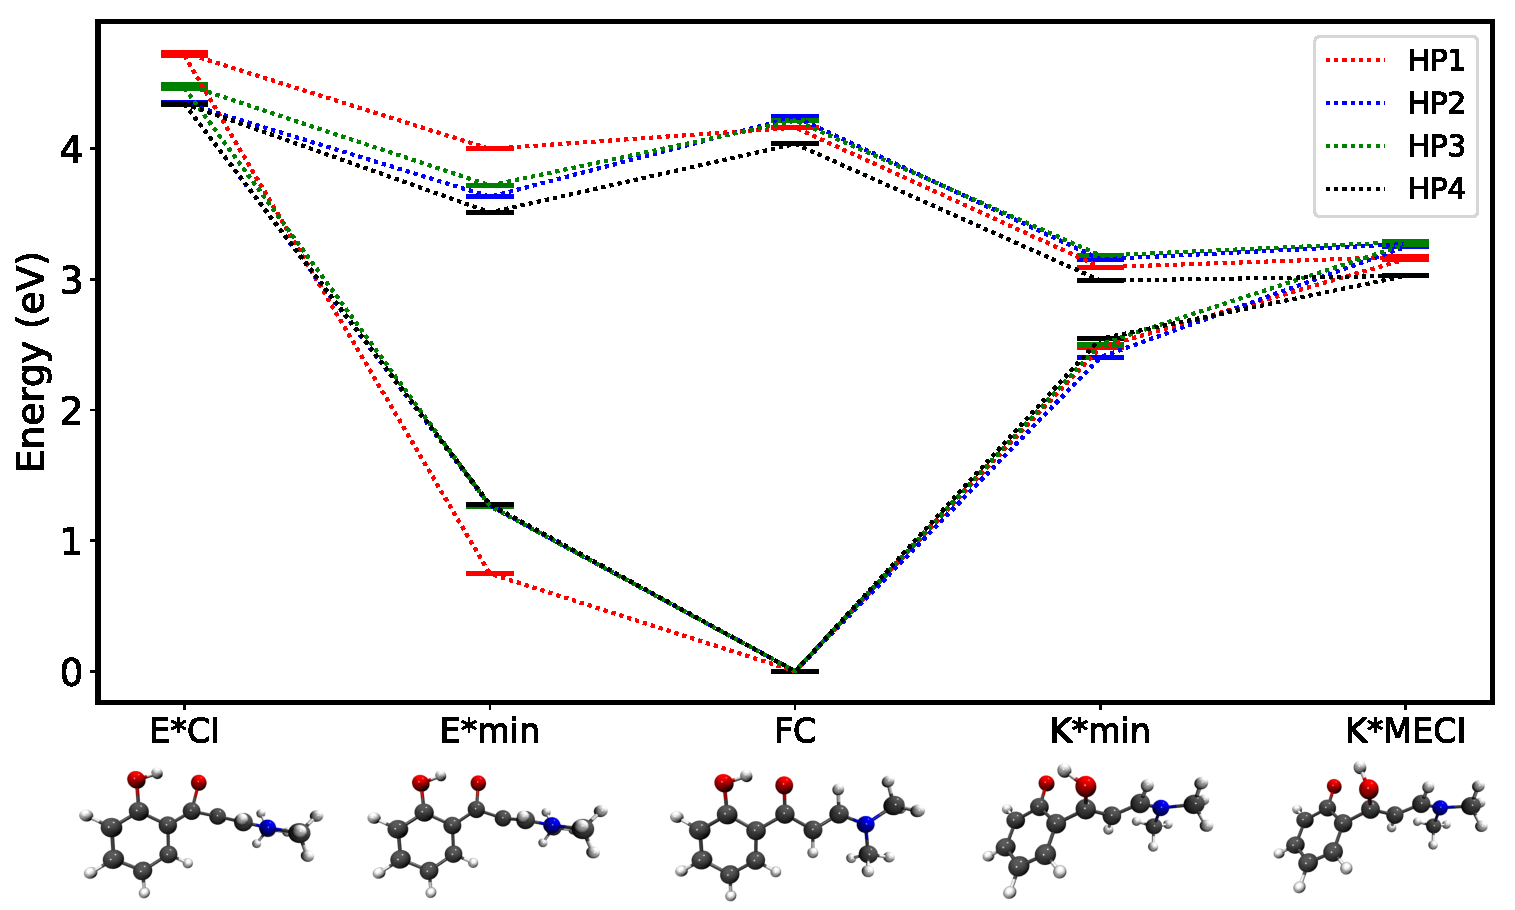
\includegraphics[width=0.8\linewidth]{5ConnectingCrystalStructure/2HP_energies_vac.pdf}
  \caption[The vacuum PES of HP\textbf{1}-\textbf{4} with TDDFT]{The critical points on the \ac{PES} for \textbf{HP}\textbf{1}-\textbf{4} obtained at (TD-)$\omega$BX-D/6-311++G(d,p) in vacuum. Also shown are the optimised geometries at each point for \textbf{HP1}.}
  \label{figure: HP_energies_vac}
\end{figure}

In Figure \ref{figure: HP_energies_vac}, the energy levels of the key regions of the \ac{PES} are shown for \textbf{HP1}-\textbf{4}. Vertical excitation to \sone{} in vacuum is predicted at 4.16 eV for \textbf{HP1}, a blue shift of 0.51 eV compared to \textbf{HC1}.  There is a blue shift of 0.09 eV for \textbf{HP2} and a red shift of 0.18 for \textbf{HP4} compared to \textbf{HP1}. These excitations are all  bright and HOMO-LUMO in character. The difference density plots show that density is lost from the phenol oxygen and donated to the C=O carbonyl, as for \sone{} in \textbf{HC5} (Figure \ref{figure: monomer_excitations}). Results from Chapter \ref{chapter:NRdecay} show that this electronic structure promotes ESIPT. In \textbf{HP2} and \textbf{HP3}, there is some donation from the amino N. In \textbf{4}, electron density is lost from the fluorine. 

The experimental absorption in DCM is centred at 3.43 eV for \textbf{1}, and thus the TDDFT excitation energies are largely overestimated. When a solvent cavity is introduced through the \ac{PCM}, the \sone{} energy is red shifted to 4.01 eV - an improvement but still largely overestimated compared to experiment. Another \ac{RSH} functional, CAM-B3LYP,\cite{Yanai2004} performs little better, with the bright state at 3.98 eV.  It is for this reason that in the solid state calculations in Section \ref{section: Connecting_Relaxation}, the CASPT2 method is applied to determine the energetic pathways.
\begin{figure}[t]
\centering
  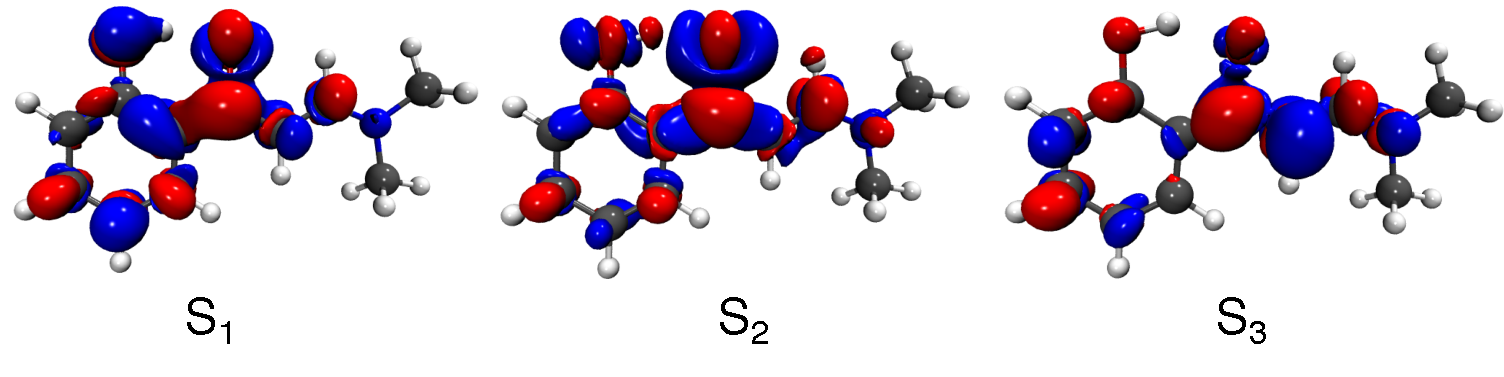
\includegraphics[width=0.9\linewidth]{5ConnectingCrystalStructure/monomer_excitations.pdf}
  \caption[Electron density difference maps for the first three excitations of \textbf{HP1}.]{Electron density difference maps for the first three excitations of \textbf{HP1}. Blue regions represent electron density loss from the ground state and red represent electron density gain in the excited state, with isovalue of 0.002. Calculated at TD-$\omega$B97X-D/6-311++G(d,p) in vacuum.}
  \label{figure: monomer_excitations}
\end{figure}

In the enol channel relaxation is not \textit{via} rotation about $\theta_{tor}$, instead occurring through partial cis-trans isomerisation about the carbon-carbon double bond. Fluorescence from this state is dipole forbidden with negligible oscillator strength. The conical intersection on the enol channel is inaccessible, with a distortion of the carbonyl group. 

The relative energetic stability of the keto channel is expected to result in a large bias and high population of \Kstar{}. As for the \textbf{HC} systems, relaxation is \textit{via} rotation about $\theta_{tor}$ (defined in Figure \ref{figure: dihedral_scans_vac}) and is heavily favoured, as shown by the relaxed geometry scan of $\theta_{tor}$ in Figure \ref{figure: HP_scan_vac}. There is destabilisation of the ground state through the rotation but the keto state remains stable through 180\degree{}. We shall return to this concept in Section \ref{section: Connecting_Bias}. Full isomerisation is not expected due to the high energy of the trans-keto state in both \sone{} and \szero{} compared to the cis-keto conformer. The conical intersection is energetically accessible in vacuum, with the substituent effects relatively minor. This is to be expected, since experimental results show that both absorption and emission energies show only minor (\textless{} 0.15 eV) substituent dependence. 

\begin{figure}[t]
\centering
  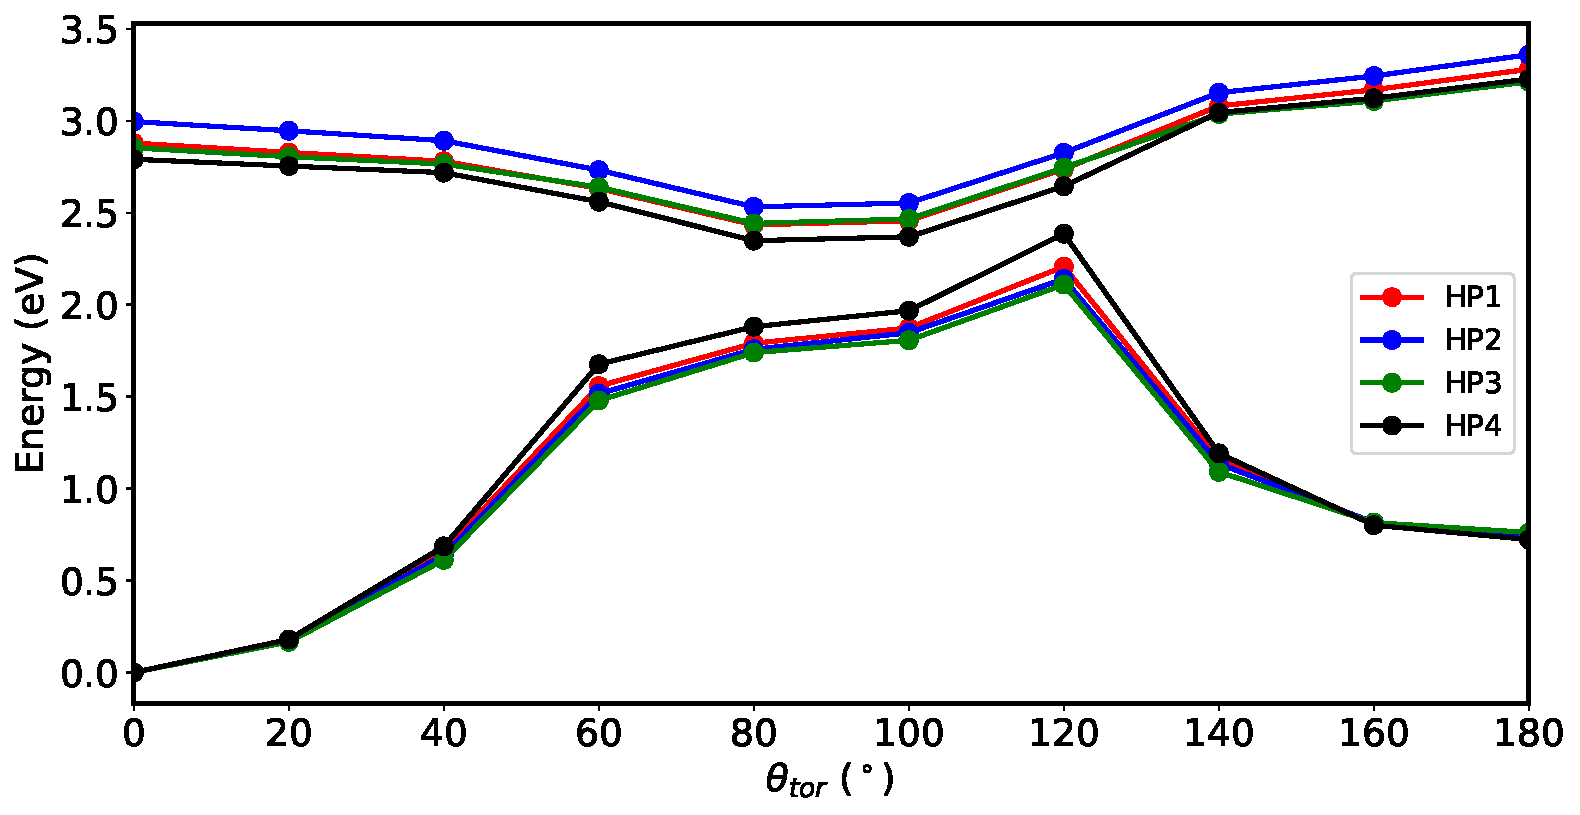
\includegraphics[width=0.9\linewidth]{5ConnectingCrystalStructure/2HP_scan_vac.pdf}
  \caption[Relaxed geometry scan of $\theta_{tor}$ for \textbf{HP} derivatives]{Relaxed geometry scan of $\theta_{tor}$ for \textbf{HP1}-\textbf{4}, calculated at TD-$\omega$B97X-D/6-31G(d) level of theory in vacuum.}
  \label{figure: HP_scan_vac}
\end{figure}
%%%%%%%
%%%%%%%
\subsection{\textbf{HP} Bias for ESIPT}\label{section: Connecting_Bias}
%%%%%%%
%%%%%%%
In this section, it is shown that the \Kstar{} population is enhanced by the inherent bias for ESIPT in the \textbf{HP}s compared to the \textbf{HC}s. The electronic densities show that in the bright excitation of \textbf{HC1}, electron density is mainly donated from the unsaturated bridge and the dimethylaniline moiety (Figure \ref{figure: monomer_excitations}). In contrast, in \textbf{HC5} and to a greater extent \textbf{HP1} (due the removal of the second aryl group), electron density is decreased at the phenol oxygen in the excited state (Figure \ref{figure: HC_Vac_Densities}). NBO charge analysis of the phenol oxygen shows that $\Delta$q increases from +0.01 to +0.05 to +0.09 for \textbf{HC1}, \textbf{HC5} and \textbf{HP1} respectively. This increases the bias for ESIPT in \textbf{HC5} and \textbf{HP1} due to the increased acidity of the transferring proton, as shown by the excited state PES relaxed geometry scan in Figure \ref{figure: Hscan}. \textbf{HP1} shows a stabilisation of 0.62 eV, compared to 0.48 eV for \textbf{HC5} and 0.38 for \textbf{HC1}. 

\begin{figure}[t]
\centering
  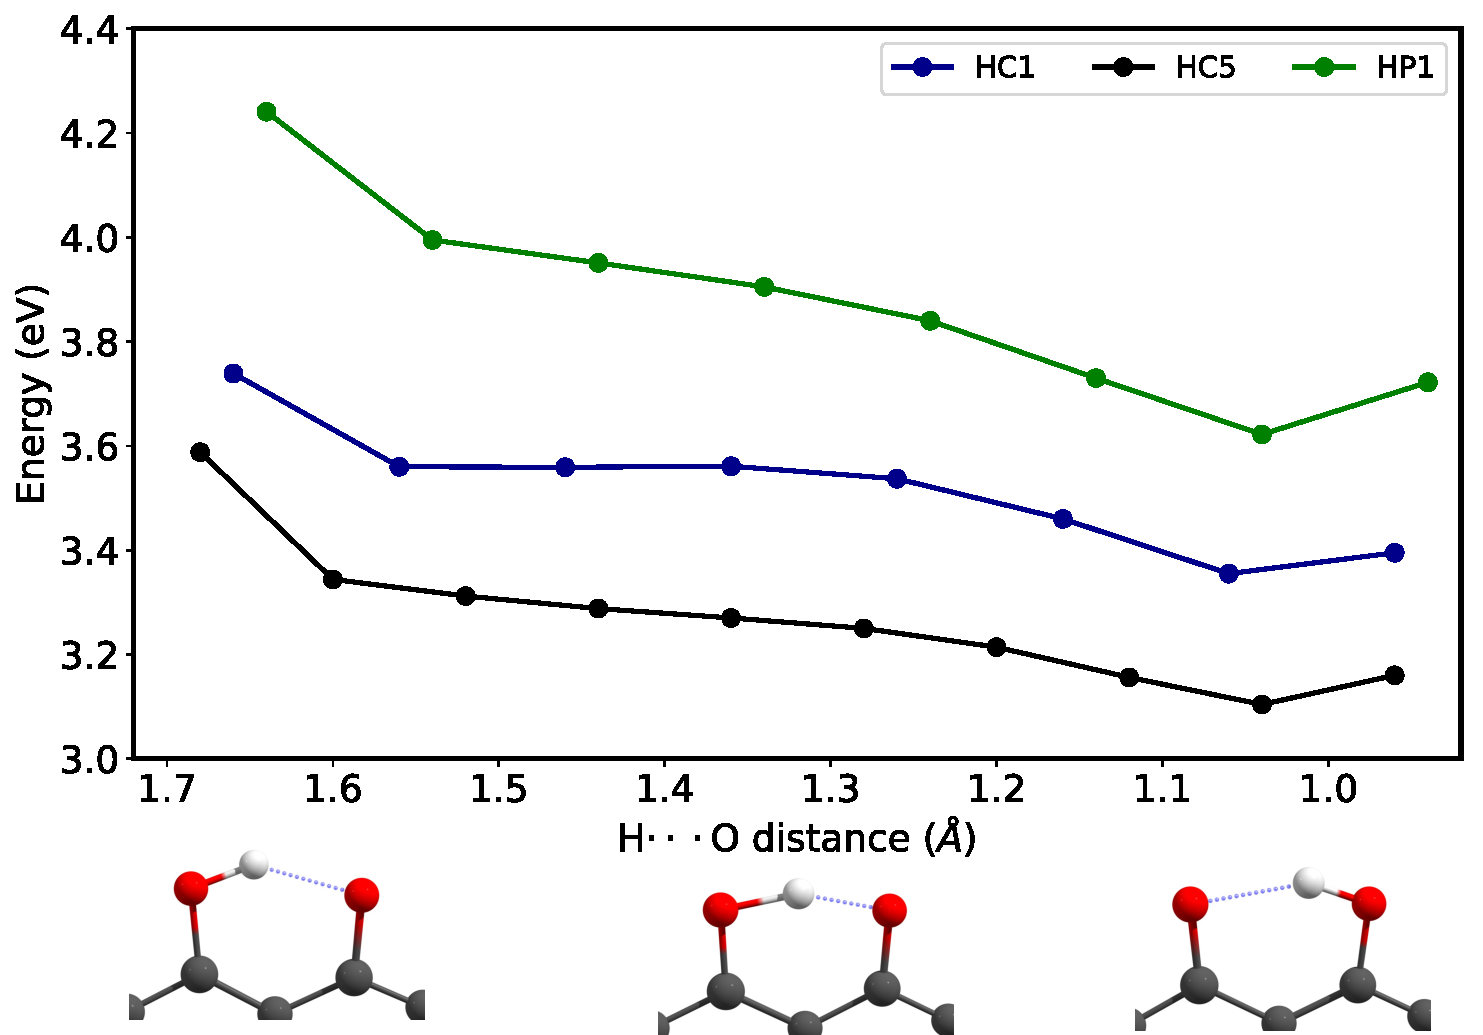
\includegraphics[width=0.8\linewidth]{5ConnectingCrystalStructure/Hscan}
  \caption[Relaxed geometry scan for ESIPT process.]{Relaxed geometry scan of the phenol hydrogen to carbonyl oxygen distance for \textbf{HC1}, \textbf{HC5} and \textbf{HP1}, calculated at TD-$\omega$B87X-D/6-31G(d).}
  \label{figure: Hscan}
\end{figure}

In the \Kstar{} channel in vacuum, relaxed geometry scans along the torsional relaxation mode (Figure \ref{figure: dihedral_scans_vac}) show that for \textbf{HC5}, the onset of the conical intersection seam is reached at 60\degree, due to the overload of electronic density at the protonated carbonyl group. Contrastingly in \textbf{HP} systems, the conical intersection seam is not found along torsional relaxation mode. While the electronic density distribution in \textbf{HP} systems leads to a strong bias for ESIPT, as for \textbf{HC5}, it does not destabilise the ground state during rotation to the same extent. \textbf{HP} systems are thus inherently more stable in the \Kstar{} channel. However, for all \textbf{HC} and \textbf{HP} systems, the MECI in non-aggregated form is energetically accessible post photoexcitation and thus nonradiative decay is witnessed experimentally. The proton lability in the \textbf{HP} systems, on account of electron density distribution, and the stability of the \Kstar{} minimum, means they obey design rule one more strictly than in the \textbf{HC} systems. 

\begin{figure}[t]
\centering
  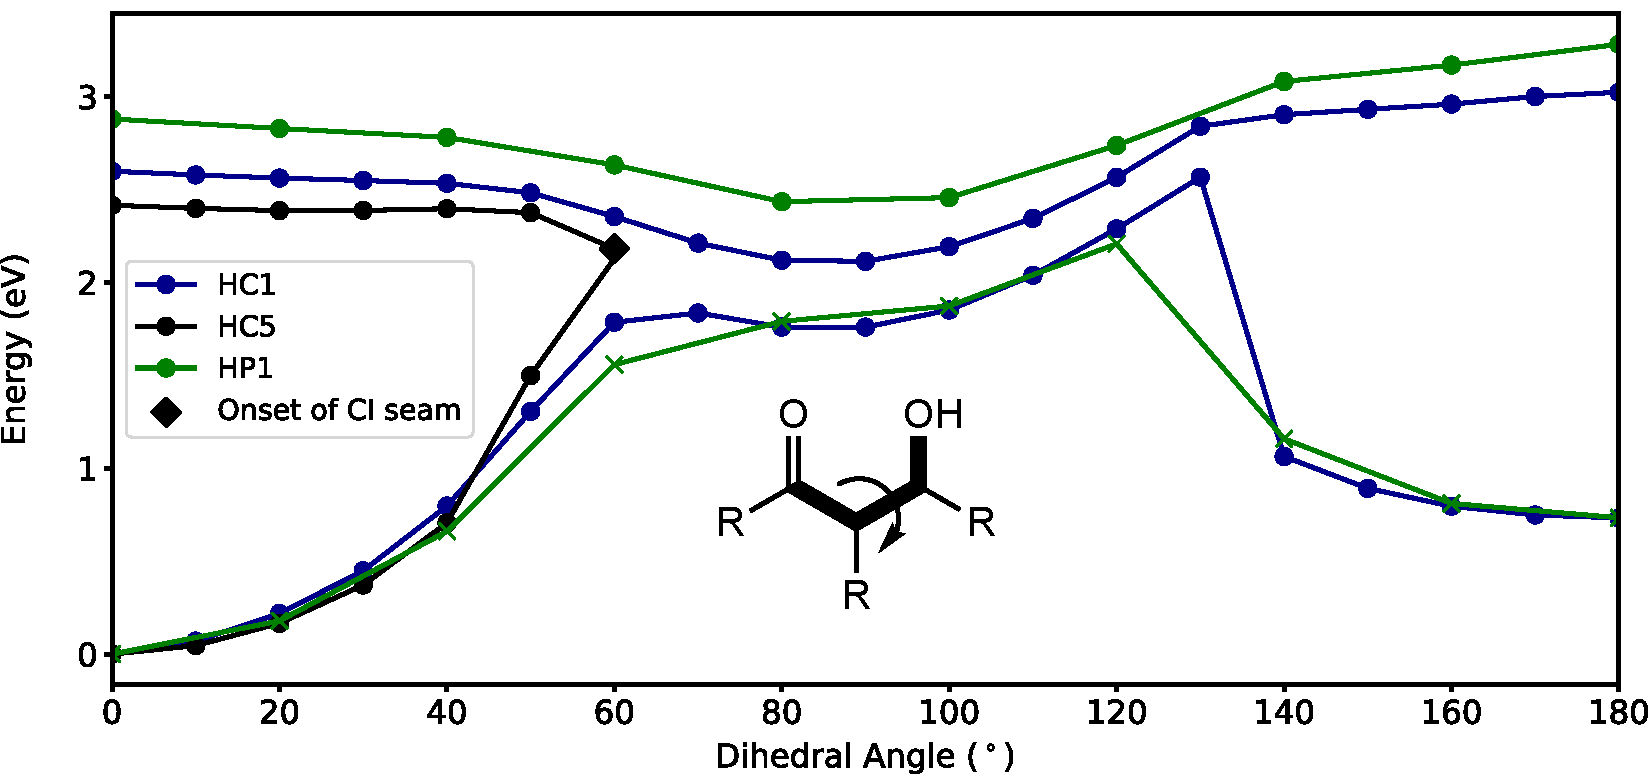
\includegraphics[width=0.8\linewidth]{5ConnectingCrystalStructure/dihedral_scans_vac}
  \caption[Relaxed geometry scan of the torsional angle]{Relaxed geometry scan of the torsional angle (shown inset, $\theta_{tor}$)  for \textbf{HC1}, \textbf{HC5} and \textbf{HP1} in vacuum, calculated at TD-$\omega$B87X-D/6-31G(d). For \textbf{HC5}, the scan cannot proceed further than 60\degree{} due to the convergence of the two electronic states.}
  \label{figure: dihedral_scans_vac}
\end{figure}

%%%%%%%%%%%%%%%%%%%%%%%%
%%%%%%%%%%%%%%%%%%%%%%%%
\subsection{Relaxation Pathways in the Molecular Crystal}\label{section: Connecting_Relaxation}
%%%%%%%%%%%%%%%%%%%%%%%%
%%%%%%%%%%%%%%%%%%%%%%%%
Results from Chapter \ref{chapter: Inter} showed that efficient population transfer to the \Kstar{} tautomer is only one prerequisite for fluorescence. The accessibility of the nearest conical intersection can dictate the luminescent response. For \textbf{HC1}, fluorescence is possible due to the high energy conical intersection in the solid state. On the other hand, for \textbf{HC5}, whilst ESIPT is more efficient than in \textbf{HC1}, the \ac{QE} is essentially zero and AIE is not seen. This can be attributed to dominance of nonradiative decay as a result of a low-lying MECI being classically accessible post electronic excitation. While intermolecular factors play a role in the conformation of the MECI, the energetic accessibility is determined by the electronic structure of the chromophore. To asses the accessibility of the MECI in the solid-state in \textbf{HP1}, we construct the excitation-decay pathway in the using QM:MM cluster models. The calculated PES for \textbf{HP1} in vacuum and the solid state is shown in Figure \ref{figure: HP1_crystal_vs_vac}.
Geometries were optimised at the Franck-Condon, the \Kstar{} minimum and the MECI with (TD-)$\omega$B97X-D/6-31+G(d):AMBER using a trimer chromophore. The central monomer, where ESIPT and the MECI occur, was then used as the chromophore in MS-3-CASPT2(12,11)/6-31G(d):AMBER single point calculations, with the two other members of the trimer demoted to the MM-level. This eased the computational expense in the MS-3-CASPT2(12,11):AMBER calculations, which are necessary to accurately predict the energy of the \sone{} excitation in the solid state. The MECI geometry obtained with the trimer with TD-DFT compares well with the geometry obtained at MS-2-CASSCF(12,11):AMBER, with an \ac{RMSD} of 0.08(9) \AA{} . With the monomer model, the \ac{RMSD} is 0.09(2) \AA{} .
%%%
\begin{figure}[t]
\centering
  \includegraphics[width=0.9\linewidth]{5ConnectingCrystalStructure/HP1_crystal_vs_vac}
  \caption[PES for \textbf{HP1} in vacuum and the solid state]{Calculated energies and geometries at critical points on PES. Geometries obtained with (TD)-$\omega$B97X-D/6-31G(d)(:AMBER), with energies calculated at MS-3-CASPT2(12,11):(AMBER). The average energy of the \sone{} and \szero{} states is shown for the MECI.}
  \label{figure: HP1_crystal_vs_vac}
\end{figure}
%%%

At the MS-3-CASPT2(12,11)/6-31G(d):AMBER level, absorption for \textbf{HP1} is calculated at 3.67 eV (\textit{f}=0.868), in fair agreement but blue-shifted by 0.41 eV compared with the crystalline absorption maximum of 3.26 eV.\cite{Tang2016} 
With a four-state average (MS-4-CASPT2), this improves further to 3.52 eV. With TD-$\omega$B97X-D/6-31G(d):AMBER, the bright state is calculated at 4.25 eV in the trimer model and 4.23 eV in the monomer model, a large overestimation of the absorption energy. When the 6-311++G(d,p) basis set is used, the prediction is slightly improved with the bright state occurring at 4.10 eV. With TD-CAM-B3LYP/6-31G(d):AMBER, the bright state is 4.20 eV. The accurate prediction of the initial photoabsorption is crucial in understanding the excited state mechanism and as such we proceed with using MS-3-CASPT2(12,11)/6-31G(d):AMBER for the energies (which is denoted CASPT2 for brevity). %perhaps the gap between s1 and s2 can be discussed

Post photo-excitation, relaxation in \sone{} \textit{via}  ESIPT is expected to be dominant relaxation channel in \textbf{HP1} due to the negligible oscillator strength (\textit{f}=0.016) of the \stwo{} state, which is n$\pi^\ast{}$ in character. Fluorescence in the molecular crystal is centred at 2.34 eV, thus displaying a Stokes shift of 0.94 eV. The emission wavelength predicted at CASPT2 is 2.73 eV, again in fair agreement and with similar blue-shift as calculated for absorption. Certainly, allowing relaxation of the exterior atoms and mutual polarisation would allow further geometric relaxation and a more accurate emission energy. Also, addition of Ewald point charges to reflect the periodicity of the crystal would improve emission further. However, this was outside the scope of the current work.
%The Stokes-shift is underestimated compared to experiment by 0.5 eV, which can be partially attributed to the frozen MM atoms and neglect of charge relaxation in the excited state.

The MECI in \textbf{HP1} lies 1.46 eV above the \Kstar{} minimum and 1.08 eV above the bright absorption state. As such, it is classically inaccessible and \textbf{HP} emission can be attributed to the trapping of the excited state at the \Kstar{} minimum, followed by radiative decay. The degeneracy of the \sone{} and \szero{} states on going from CASSCF to CASPT2 is lifted slightly, with a gap of 0.2 eV at CASPT2 level. As the substituent effects in the crystalline samples are minor in the \textbf{HP} samples (absorption and fluorescence), it can be assumed that this mechanism can be applied to all four systems in the family. It would be of interest to synthesise a \textbf{HP} system with a methoxy group the \textit{para} position, as in \textbf{HC5}, to assess its AIE behaviour.

In Figure \ref{figure: MECI_comparison}, the MECI geometries of \textbf{HC1}, \textbf{HC5}, and \textbf{HP1} are compared. All three involve the pyramidalisation of the protonated carbonyl group  combined with torsional rotation of the deprotonated phenol moiety. In \textbf{HC1} and \textbf{HP1}, the compounds which undergo AIE due to the high energy of the MECI, the torsional angles are 50\degree{} and 53\degree{} respectively. In \textbf{HC5}, where the MECI is energetically accessible, the pyramidal distortion is only 28\degree{}. The same effect is seen in vacuum, where the MECI of \textbf{HC5} is also onset at lesser distortion than the other systems, as discussed above. Thus the stability of the \textbf{HC5}, and the high energy MECIs of \textbf{HC1} and \textbf{HP1}, are mainly due to the electronic effects of the chromophore. Rather, the role of the packing and the crystalline environment as a whole is to promote efficient localisation of the excited state at the expense of exciton hopping the enol state, as will be investigated in Section \ref{section: Connecting_Marcus}. Such is the propensity for localisation and ESIPT in \textbf{HP} and the high energy MECI, a largely increased \ac{QE} is witnessed as a result, fulfilling design rules two and three.
%%%
\begin{figure}[t]
\centering
  \includegraphics[width=0.9\linewidth]{5ConnectingCrystalStructure/MECI_comparison.pdf}
  \caption[MECI geometries for \textbf{HC1},\textbf{HC5} \% \textbf{HP1}.]{Overlaid structures of the MECI for \textbf{HC1} (blue) and \textbf{HC5} (black), and \textbf{HP1} (green), shown from three viewpoints. Only the atoms shared by all three compounds are shown.}
  \label{figure: MECI_comparison}
\end{figure}

%%%%%
\subsection{Radiative Decay Rates}\label{section: connecting_radiative_rates}
%%%%%
In this section we calculate the emission rate $k_{r}$ for \textbf{HC1}, \textbf{HC5}, and \textbf{HP1}. This can be done either through the Einstein spontaneous emission relationship (Equation \ref{equation: Einstein_rate}) or through integrating the simulated spectrum (Equation \ref{equation: integrated_emission_rate}). The oscillator strength between \sone{} and \szero{} states at the \Kstar{} minimum is 0.549 at CASPT2 level (0.281 TDDFT trimer model, 0.331 with TDDFT monomer), indicating that emission will be bright. First, we compute the radiative decay rates from the E* and K* states using ONIOM(TDDFT) by computing the fluorescence spectrum and calculating $k_{r}$ through Equation \ref{equation: integrated_emission_rate}. The spectra for \textbf{HC1}, \textbf{HC5} and \textbf{HP1} are given in Figure \ref{figure: HC1_HC5_HP1_emission_oniom} and radiative rates for \textbf{HC1}, \textbf{HC5} and \textbf{HP1} are given in Table \ref{table: rates}.

\begin{figure}[t]
\centering
\includegraphics[width=0.8\linewidth]{5ConnectingCrystalStructure/HC1_HC5_HP1_emission_oniom}
\caption[Emission spectra in molecular crystal for 7\AA{} clusters for \textbf{HC1}, \textbf{HC5} and \textbf{HP1}]{Emission spectra in molecular crystal for 7\AA{} clusters for \textbf{HC1}, \textbf{HC5} and \textbf{HP1}, calculated at TD-$\omega$B97X-D/6-31G(d) in point charges. Single point energies were calculated for 100 initial conditions based upon a Wigner distribution of the excited state frequencies calculated at ONIOM(TD-$\omega$B97X-D/6-31G(d):AMBER) level.}
\label{figure: HC1_HC5_HP1_emission_oniom}
\end{figure}

For \textbf{HC1}, $k_{r,K*}$ is comparable with \textbf{HP1} in both E* and K*. However, \textbf{HC1} exhibits lower quantum efficiency, owing to the competing exciton hopping in the enol state, which will inhibit localisation and thus ESIPT. Thus in \textbf{HC1} there is competition between delocalisation, emission from E*, and emission from K*. Due to the proximity of the E* band to the absorption, only K* fluorescence will significantly contribute to the quantum yield.

For \textbf{HP1}, emission from E* is negligible and emission is expected from the K* state. The highly distorted E* minimum, is expected to play little role in the photochemistry and population transfer to K* should dominate. The radiative rate from K* is of similar magnitude to \textbf{HC1}, and as such the higher quantum yield of \textbf{HP1} is on account of the lower nonradiative decay rate and lack of other competitive pathways, such as exciton hopping. In Table \ref{table: rates}, given in parenthesis are the rates obtained from the more simple Einstein relationship. This method compares well to the more complex spectral method, where the Wigner distribution of geometries based on harmonic frequencies should provide a more realistic radiative rate. Based on these rates the Einstein relationship can provide a qualitative estimate for $k_{r}$ without the need for computing the fluorescence spectrum, which is a far more computationally demanding approach. However, that is most likely due to the fact that in these systems, the steric hindrance of the molecular crystal means there is little geometric relaxation and the excited state \ac{PES} resembles the ground state \ac{PES}, since there is not the steric freedom to explore outside of the harmonic potential.

\begin{table}
\centering
\caption[Radiative decay rates in the solid state]{Radiative decay rates $k_{r}$ in the solid state in the enol (\Estar{}) and keto (\Kstar{}) regimes for \textbf{HC1}, \textbf{HC5}, \textbf{HP1} calculated through spectral integration. In parenthesis is the rate calculated \textit{via} the Einstein relationship of Equation \ref{equation: Einstein_rate}. All rates in \SI{}{s^{-1}}.} 
\label{table: rates}
  \begin{tabular}{ccc}
    \hline
  	System & $k_{r,E*}$ & $k_{r,K*}$\\
    \hline
    \textbf{HC1} & \SI{4.68e8}{}  (\SI{1.78e9}{}) & \SI{2.99e8}{} (\SI{2.83e8}{}) \\ 
	\textbf{HC5} & - & \SI{9.54e7}{} (\SI{1.02e8}{})\\
	\textbf{HP1} & \SI{5.58e6}{} (\SI{4.49e6}{}) & \SI{1.10e8}{} (\SI{1.23e8}{}) \\
    \hline
  \end{tabular}
\end{table}
%%%%%%%%%%%%%%%%%%
%%%%%%%%%%%%%%%%%%
\subsection{Huang-Rhys Factors}\label{section: HR}
%%%%%%%%%%%%%%%%%%
%%%%%%%%%%%%%%%%%%
As discussed in Section \ref{section: lom HR}, reorganisation energies and \acf{HR} factors are often used to qualitatively account for the \ac{FGR-RIM} interpretation of \ac{AIE}. In this section we address this model for the \textbf{HC} and \textbf{HP} systems.  The \ac{HR} factors in vacuum and molecular crystals were calculated for \textbf{HC1}, \textbf{HC5}, and \textbf{HP1}. In vacuum, ground and excited states were optimised at (TD-)$\omega$B97X-d/6-31G(d) level. In the molecular crystal, a cluster model consisting of a central chromophore and all molecules within a 7\AA{}, taken from the optimised unit cell for each system. Ground and excited states were optimised at ONIOM((TD-)$\omega$B97X-d/6-31G(d):AMBER) level, and frequencies were calculated at (TD-)$\omega$B97X-d/6-31G(d) level using point charge embedding. The DUSHIN program was used to calculate the Huang-Rhys factors and the associated reorganisation energies ($\lambda_{NM}$).\cite{Reimers2001}

For \textbf{HP1} and \textbf{HC5}, it is found that $\lambda_{NM}$ overestimates the reorganisation energy with respect to $\lambda_{A}$. In \textbf{HP1},  $\lambda_{A}$ is 1.24 eV compared to 2.19 eV for $\lambda_{NM}$. In \textbf{HC5}, the NM approximation is 0.4 eV larger than $\lambda_{A}$. In both \textbf{HP1} and \textbf{HC5}, the HR factors are reduced in moving from vacuum to the solid state, in particular for rotational modes. The RIM interpretation of AIE prescribes that switch-on of fluorescence upon aggregation is due to dampening of rotational modes, which dissipate the excited state nonradiatively, as witnessed by a reduction in the HR factors. While \textbf{HC1}, \textbf{HC5} and \textbf{HP1} show this effect, \textbf{HC1} and \textbf{HP1} show AIE while \textbf{HC5} is dark in both dispersed and aggregated forms. The dampening of the HR factors does not result in luminescence in \textbf{HC5}, suggesting that the excited state wavepacket decays through the MECI.\cite{Dommett2017} Furthermore, due to the anharmonicity of the PES, the validity of the scheme in these cases is not clear. To explore this further, Figures \ref{figure: HC1_DUSHIN}-\ref{figure: HP1_DUSHIN} show the Huang-Rhys (HR) factors in vacuum and solid state for \textbf{HC1}, \textbf{HC5} and \textbf{HP1}. The different y-axis scales for the Huang-Rhys factors between plots should be noted. Each system is discussed in turn below.

For \textbf{HC1} in vacuum (Figure \ref{figure: HC1_DUSHIN}, left), the geometric similarity between the planar E* excited state minimum and the ground state equilibrium geometry yields negligible HR factors. This leads to $\lambda_{NM}$ of 0.08 eV, which underestimates the $\lambda_{A}$ of 0.36. For K*, the PES in vacuum is highly anharmonic, and intramolecular rotation leads to a highly distorted geometry with respect to the ground state. As a consequence, the HR factors are extremely large and the harmonic approximation is not applicable for determining the reorganisation energy, as illustrated by a value of 99 eV ($\lambda_{A}$=3.64 eV). Moving to the molecular crystal (Figure \ref{figure: HC1_DUSHIN}, right), in E* the HR factors are of similar magnitude as in vacuum but in K* they are markedly reduced and suppressed to fractional values. The largest K* HR factor is the O-H stretching mode, since the geometry remains planar and has the largest displacement between \szero{} and \sone{} as it is the ESIPT coordinate. The K* $\lambda_{NM}$ is 4.67 eV, with $\lambda_{A}$=0.59 eV. 

\begin{figure}[t]
\centering
  \includegraphics[width=\linewidth]{5ConnectingCrystalStructure/HC1_DUSHIN}
  \caption[HR factors for \textbf{HC1}]{Huang-Rhys factors associated with each normal mode calculated \textit{via} the Duschinsky rotation matrix between the E* and \szero{}, and K* and \szero{} electronic states for \textbf{HC1}. Frequencies 0-500 cm\textsuperscript{-1} in the solid state are shown in the inset.}
  \label{figure: HC1_DUSHIN}
\end{figure}

\begin{figure}[t]
\centering
  \includegraphics[width=\linewidth]{5ConnectingCrystalStructure/HC5_DUSHIN}
  \caption[HR factors for \textbf{HC5}]{Huang-Rhys factors associated with each normal mode calculated \textit{via} the Duschinsky rotation matrix between  K* and \szero{} electronic states for \textbf{HC5}. Frequencies 0-500 cm\textsuperscript{-1} in the solid state are shown in the inset.}
  \label{figure: HC5_DUSHIN}
\end{figure}

\begin{figure}[t]
\centering
  \includegraphics[width=\linewidth]{5ConnectingCrystalStructure/HP1_DUSHIN}
  \caption[HR factors for \textbf{HP1}]{Huang-Rhys factors associated with each normal mode calculated \textit{via} the Duschinsky rotation matrix between K* and \szero{} electronic states for \textbf{HP1}. Frequencies 0-500 cm\textsuperscript{-1} in the solid state are shown in the inset.}
  \label{figure: HP1_DUSHIN}
\end{figure}

In \textbf{HC5} there is no stable E* minimum in either vacuum or the solid state for the monomer chromophore. In vacuum, the HR factors are much less than in \textbf{HC1} due to the rotation angle at the minimum being less distorted. The molecule is more planar and is closer in structure and vibrational signature. At larger rotation angles the MECI is reached. HR factors are reduced in the solid state, in particular for the rotational modes, but with the O-H stretch HR factor increasing.   %Here the OH stretch is at 2036 cm\textsuperscript{-1}. In the molecular crystal the OH-

For \textbf{HP1}, large reorganisation energies, and correspondingly large HR-factors, are associated with low-frequency rotational modes. Indeed, such is the displacement between modes in the ground and excited states, the total reorganisation energy is 41 eV, whereas the adiabatic value 3.89 eV. As such, the harmonic approximation is invalid here due to the excited state potential energy surface anharmonicity. In the solid state, the normal modes associated with rotation are significantly reduced, whilst the largest HR factor is associated with the stretching of the phenol oxygen. This is to be expected, since it is along this coordinate that ESIPT occurs, and hence is has the largest HR-factor. In solid state, $\lambda_{NM}$ is 2.19 eV, compared with $\lambda_{A}$ of 1.24 eV.  

In the case of the \textbf{HC} and \textbf{HP} systems, the AIE behaviour can not be directly attributed to the reduction of the HR factors in the solid state compared to vacuum. Such is the complexity of the PES, where ESIPT and rotation occur in the excited state (in vacuum), the surfaces are highly anharmonic and the validity of the \ac{FGR-RIM} scheme is not clear. As such, it is not the focus of our investigation into the AIE behaviour of these systems.

%%%%%%%%%%%%%%%%%
\subsection{Analysis of Crystal Packing} \label{section: Connecting_Motifs}
%%%%%%%%%
%%%%%%%%%
In this section we use several techniques to analyse the crystal structures of the eleven compounds of Table \ref{table: chalcones}. The crystalline environment of each crystal is examined initially from the perspective of a monomeric chromophore. To this end, we use Voronoi cell volumes $V_{cell}$ and van der Waals volumes $V_{vdW}$ to determine a Voronoi index $V_{i}=V_{cell}/V_{vdW}$, a metric indicating the normalised accessible volume for a monomer in the crystal. $V_{i}$ values (Figure \ref{figure: voronoi_index}) range from 1.29-1.48, showing that despite the substituent and packing differences, the each monomer in the system has between 30\%-50\% of its van der Waals volume to freely vibrate, rotate or translate. For the \textbf{HC} systems, the average $V_{i}$ is 1.36$\pm$0.06, and 1.30$\pm$0.01 for the \textbf{HP} systems. The accessible volume for the \textbf{HC} systems shows greater variation but is overall slightly higher than for the less varied \textbf{HP} systems. The increased volume for the \textbf{HC} systems theoretically allow for greater nuclear relaxation in the excited state. However, reorganisation energies (Section \ref{section: Connecting_Marcus}) for the \textbf{HP} systems are larger than for \textbf{HC}, showing the importance of the electronic effects over geometric considerations. 
\begin{figure}[t]
\centering
  \includegraphics[width=0.8\linewidth]{5ConnectingCrystalStructure/Voronoi_Index}
  \caption{Voronoi indices for \textbf{HC} and \textbf{HP} crystal structures.}
  \label{figure: voronoi_index}
\end{figure}

Exciton transport has been occurs through hopping between molecular sites, and thus it is important to understand the possible intermolecular transport channels in the \textbf{HC} and \textbf{HP} systems.\cite{Bredas2004} To determine the intermolecular relationships, we examine the topology of the molecular crystals of \textbf{HC} and \textbf{HP} families by considering dimer configurations. Crystal morphologies are commonly described qualitatively as herringbone, face-face, edge-tail, \textit{etc}. Here we take a more of quantitative approach by constructing maps of each crystal, based on a geometric description of the dimers. These maps allow the topology of the crystal to be analysed graphically.


Dimers are quantified through three angle variables, $\alpha$, $\beta$, and $\gamma$. These are depicted in Figure \ref{figure: dimer_schematic_alpha}, and example dimers with associated angles are given in Figure \ref{figure: motif_examples}. Three axes, $x$, $y$, $z$, are defined on each molecule $i$ and $j$ of the dimer, where $x$ and $y$ are the long and short axes of the molecule, and $z$ is the orthogonal vector. These vectors comprise an orthogonal basis to describe the dimer. The angles are then defined as:
\begin{itemize}
\item[$\bullet$] $\alpha$: The azimuthal angle between the monomers shown as the black angle in Figure \ref{figure: dimer_schematic_alpha}. Calculated as the angle between the $z$-axis located at the centroid of monomer $i$, and the vector connecting two centroids. $\alpha$ is calculated twice, once with each monomer as the reference. The smallest angle is chosen, such that 0\degree{}$\leq\alpha\leq{}90\degree{}$.

\item[$\bullet$] $\beta$: The angle between the two short-axis vectors $y$ of each molecule, shown in green in Figure \ref{figure: dimer_schematic_alpha}. $\beta$ ranges from 0\degree{} to 180\degree{}, tracking whether monomers are aligned cofacially parallel ($\beta=$0\degree{}, CoF-P), or cofacially antiparallel ($\beta=$180\degree{}, CoF-A), or in a herringbone edge-face manner (90\degree{}, Hb), and all configurations in between. $\beta$ is commonly described as the ``herringbone'' angle. 

\item[$\bullet$] $\gamma$: The angle between the long-axis vectors $x$, ranging from 0\degree{} (parallel, P) to 180\degree{} (antiparallel, A). At $y=$ 90\degree{}, the dimer is T- or L-shaped, dependent on the $x$-slip. 
\end{itemize}

\begin{figure}[t]
\centering
  \includegraphics[width=0.8\linewidth]{5ConnectingCrystalStructure/dimer_schematic_alpha}
  \caption[Schematic of $\alpha$, $\beta$, and $\gamma$ angles for classification of dimers.]{Panel a), left; schematic of two monomers, and the $\alpha$, $\beta$, and $\gamma$ angles used to classify dimer configurations. Panel b), right; distribution of $\alpha$ angles for dimers in \textbf{HC} and \textbf{HP} systems.}
  \label{figure: dimer_schematic_alpha}
\end{figure}

\begin{figure}[t]
\centering
  \includegraphics[width=0.9\linewidth]{5ConnectingCrystalStructure/motif_examples}
  \caption[Example dimers in \textbf{HC1}, \textbf{HC5}, and \textbf{HP1}.]{Example dimers and associated $\alpha$, $\beta$ and $\gamma$ angles in \textbf{HC1}, \textbf{HC5}, and \textbf{HP1}.}
  \label{figure: motif_examples}
\end{figure}

In Figure \ref{figure: dimer_schematic_alpha}b the distribution density of the $\alpha$ angle is shown for the cofacially stacked \textbf{HC} and \textbf{HP} systems. The distribution is heavily skewed towards 90\degree, indicating that for the majority of cofacial dimers, there is little overlap between the centroids of the monomers. As such, it can be expected that in each molecular crystal there are few dimers with the configuration required for efficient charge or energy transfer, and that transfer will occur through only a few particular dimers. 
\begin{figure}[t]
\centering
  \includegraphics[width=0.9\linewidth]{5ConnectingCrystalStructure/dimer_classification}
  \caption[Probability density maps of $\beta$ and $\gamma$ angles.]{Panel a), left; Probability density map of the $\beta$ and $\gamma$ angles for \textbf{HC} (top) and \textbf{HP} (bottom) dimers. Key configurations are labelled on the axes, as explained in the text. Panel b), centre; probability density for the subset of dimers where $\alpha$ \textless{}  60\degree{}.  Panel c), right; probability density for the subset of dimers where $\alpha$ \textgreater{} 60\degree{}.}
  \label{figure: dimer_classification}
\end{figure}

Figure \ref{figure: dimer_classification} shows the dimer distribution densities for the $\beta$ and $\gamma$ angles for \textbf{HC} (top row) and \textbf{HP} (bottom row). Key regions are highlighted as an example in the upper plot of panel a); for example at $\beta$=90,$\gamma$=0, a herringbone (Hb) stack is witnessed with the long axes arranged in parallel. For both \textbf{HC} and \textbf{HP} systems, the majority of dimers have $\beta$ and $\gamma$ angles close to 180\degree{} (top right of plot), indicating that the most common dimer configuration is a cofacial arrangement where the carbonyl groups align antiparallel, at opposing ends of the molecule from each other. This results in an antiparallel alignment of the \sone{} transition dipole moment of each monomer.  However, as panels b) and c) show, when the $\alpha$ angle is used as a filter, the configurations with more acute azimuthal angles are mostly herringbone in nature for \textbf{HC}, with carbonyl groups at the same ($\gamma=$0\degree) or opposite ends of the dimer ($\gamma=180\degree$). There also exist dimers close to this arrangement, with deviations in both $x$ and $y$. In the relatively few \textbf{HP} systems with  $\alpha$\textless{60}\degree{}, configurations lie on the diagonal between herringbone and cofacial.

The cofacial arrangements favoured by the Kasha model occur at large slip displacements in the $x$ or $y$  plane ($\alpha$\textgreater{60}), and are more like edge-edge coplanar arrangements rather than the well-known $\pi$-stack. Only in \textbf{HC5} is there significant cofacial $\pi$-stacking between dimers, with other cofacial arrangements in \textbf{HC} and \textbf{HP} having larger $x$-slip, as is common for aromatic groups. For \textbf{HC} compounds, 63\% of the cofacially aligned dimers have a $x$-slip of less than half a molecule, whereas 68\% of cofacially-aligned \textbf{HP} dimers have a $x$-slip of more than half a molecule, as shown in Figure \ref{figure: xslip_density}. So while the cofacial, $\pi$-stacked arrangement is rare for both families, it is more prominent in \textbf{HC} compounds than their mono-aryl \textbf{HP} counterparts. The cofacial arrangement is particularly dominant in \textbf{HC5}.


\begin{figure}[t]
\centering
  \includegraphics[width=0.8\linewidth]{5ConnectingCrystalStructure/xslip_density}
  \caption[$x$-slip densities for dimer configurations of \textbf{HC} and \textbf{HP} systems]{The density of slip distances for each molecular dimer in the $x$-plane (long axis) for cofacial dimers. The slip is normalised by the length of the long axis $x$ for each molecule, such that slip is molecule independent.}
  \label{figure: xslip_density}
\end{figure}

Overall, the significant dimer arrangement in \textbf{HP} compounds is a herringbone structure, with the majority of cofacial arrangements having a large $x$ or $x$-slip with minimal $\pi\pi$ interactions due to the single aryl groups aligning at $y$=180\degree. The $\alpha$ angle is generally larger than in \textbf{HC}, indicating a larger slip, with overlapping monomers distributed around a cofacial stacking. The prominence of the herringbone arrangement in \textbf{HC} systems is replaced by a propensity for a T-shape packing, quantified by the $\gamma$ angles distributed around 90\degree. In the next section, we show how these geometric parameters influence the exciton coupling in the \textbf{HC} and \textbf{HP} families.

\subsection{Intermolecular Interactions in the Molecular Crystal}\label{section: Connecting_Interactions}

Localisation of the electronic excited state onto one monomer of the molecular crystal has been shown to be an important step in the relaxation process of ESIPT systems in the solid state in Chapter \ref{chapter: Inter}. For the dimers discussed above, the coupling $J_{ij}$ between monomers $i$ and $j$ is calculated in Troisi's diabatization scheme based on the orthogonal transformation of adiabatic states to diabatic states (Equation \ref{equation: diabatic matrix}).\cite{Arago2015,Fornari2016}. In this Chapter this method is extended to asses the effect of a third monomer $k$ on the exciton coupling, where in a trimer chromophore, $\textbf{H}^D$ becomes a 3x3 matrix
\begin{equation}
\small
\label{equation: 3x3 diabatic matrix}
\begin{bmatrix}
E_{i}^D & J_{ij} & J_{ik}\\
J_{ji} & E_{j}^D & J_{jk} \\
J_{ki} & J_{kj}& E_{k}^D
\end{bmatrix}
=
\begin{bmatrix}
C_{11} & C_{12} & C_{13}\\
C_{21} & C_{22} & C_{23}\\
C_{31} & C_{32} & C_{33}
\end{bmatrix}
\begin{bmatrix}
E_{i}^A & 0 & 0\\
0 & E_{j}^A & 0\\
0 & 0 & E_{k}^A\\
\end{bmatrix}
\begin{bmatrix}
C_{11} & C_{12} & C_{13}\\
C_{21} & C_{22} & C_{23}\\
C_{31} & C_{32} & C_{33}
\end{bmatrix}
\end{equation} 
where the coupling $J_{ij}$ between monomers $i$ and $j$ incorporates the effect of monomer $k$, which can quantified through comparison of the dimeric and trimeric $J_{ij}$. Analysis of excitations at the Franck-Condon geometry for a trimer chromophore show that for \textbf{HP1}, the bright state is delocalised over two of the molecules arranged in a cofacial arrangement. This is shown in Figure \ref{figure: trimer_excitations}. A delocalised state over the whole trimer is not observed. Analysis of the excitations of the three types of dimer inherent in the trimer reveal that in each case, regardless of the stacking arrangement and despite the close aggregation of monomers, the excitation is delocalised over no more than two monomers. 

\begin{figure}[t]
\centering
  \includegraphics[width=0.8\linewidth]{5ConnectingCrystalStructure/trimer_excitations}
  \caption[Electron density difference maps for the first nine excited state of the \textbf{HP1} trimer.]{Electron density difference maps for the first nine excited state of the \textbf{HP1} trimer. The same colour scheme is used as in Figure \ref{figure: HC_Vac_Densities}}
  \label{figure: trimer_excitations}
\end{figure} 

To quantify the effect of the third molecule on the exciton coupling, the exciton coupling for a trimer system was calculated in \textbf{HP1}, \textbf{HC1}, and \textbf{HC5}. It is found that the addition of a third molecule has only a small effect on the dimer coupling in \textbf{HP1} and \textbf{HC1}, where the increased coupling in one dimer is compensated for by the decreased coupling in the other dimer, with difference of less that 0.02 eV. The largest effect is seen in \textbf{HC5} due to the cofacial packing of the trimer system, where the central monomer is sandwiched by two cofacially stacked monomers, one parallel and one antiparallel, as shown in \ref{figure: trimer_couplings}. For \textbf{HC1}, two trimers are used to capture both parallel and antiparallel stacked dimers. 

These perturbations are no larger than the inherent modulation of couplings in the dynamic regime.\cite{Arago2015,Arago2016} As such, focus from here will be on dimer couplings where the presence of exterior molecules has been neglected. The exciton couplings for all dimers and the identity of the dimer with the largest $J$ are shown in Figure \ref{figure: couplings}. 
\begin{figure}[t]
\centering
  \includegraphics[width=0.8\linewidth]{5ConnectingCrystalStructure/trimer_couplings}
  \caption[Trimer exciton couplings]{Schematic of the trimers extracted from unit cells of \textbf{HC1}, \textbf{HC5} and \textbf{HP1}. Exciton couplings considering the trimer are shown. In parenthesis are the couplings considering only a dimer. Calculated at $\omega$B97X-D/6-311++G(d,p) level of theory.}
  \label{figure: trimer_couplings}
\end{figure}


\begin{figure}[t]
\centering
  \includegraphics[width=0.9\linewidth]{5ConnectingCrystalStructure/couplings}
  \caption[Exciton couplings in \textbf{HC} and \textbf{HP} systems]{Exciton couplings $J$ between monomers $i$ and $j$ in the dimers identified in \textbf{HC} and \textbf{HP}. The mean coupling is also shown, along with the distance in angstroms between the constituent monomer centroids.}
  \label{figure: couplings}
\end{figure}

In \textbf{HC1-4}, where the closest packed dimers are herringbone in nature, similar dimer configurations are present. For \textbf{HC-2}, the identity of the dimer with the largest coupling changes due to a lateral displacement of one monomer increasing the centroid distance to 8.5 {\AA} and thus reducing the coupling in the herringbone stacked dimer. The identity of the largest coupled dimer changes to a cofacial, edge-edge stacked dimer with $\alpha=87\degree$, where minimal overlap reduces the coupling $J$. For \textbf{HC-1,3,4}, the herringbone stacking pattern is exhibited where the largest coupling is found in \textbf{HC1}, where the monomers are most tightly packed. In \textbf{HC5-7}, face-face stacked dimers are more prevalent in the crystal structure. The size of the coupling in \textbf{HC6} is reduced compared to \textbf{HC5} due to the $y$ displacement of one the monomers. It is further reduced in \textbf{HC7} due to an increased $x$-slip. In the \textbf{HP} compounds, the large $\alpha$ and $x$-slip values systematically reduce the average coupling. In each \textbf{HP} derivative there exists one close packed, cofacial dimer which exhibits the largest coupling. In \textbf{HP2-3}, the crystal structures afford more efficient cofacial stacking with $x$-slip values of only 1{\AA}, resulting in the largest couplings of all investigated systems. 

As shown in  Figure \ref{figure: dimer_regressions}a, the coupling $J$ correlates linearly with half of the energy splitting for the \sone{} and \stwo{} states of the dimer. This is somewhat surprising, given the simplicity of the original model (Section \ref{section: lom intermolecular-interactions}), the polarity of the molecules in question and their generally nonparallel stacking. The energy splitting is perhaps the simplest way to obtain the exciton coupling in the Kasha regime, although it is more expensive than using atomic-centred transition charges, or the PDA approximation, since the supermolecular calculation must be done rather than one monomer calculation. At small intermolecular distances (\textless4{\AA}), these computationally efficient metrics can underestimate the couplings due to them only considering the Coulomb interaction.\cite{Kistler2013} The linear correlation here shows that the general Kasha interpretation of the coupling applies here and that the diabatization method to obtain the couplings reproduces the supermolecular coupling.

The role of H- and J-aggregates is investigated by assigning dimers based on the oscillator strength of the \sone{} (J) and \stwo{} (H) excitation, which offers better resolution than using the energy shift. This is summarised in Table \ref{table: dimer_types}. In \textbf{HC}, systems, 60\% of dimers are J-aggregates, while in \textbf{HP} systems the J-aggregate population is 58\%. For \textbf{HC-4} and \textbf{HC-5}, which are nonemissive, the J-aggregate population drops to 22\% and 32\%, respectively. Important to note, however, is that emission in \Kstar{} is from a localised excited state, and thus monomer regime should dominate the emission characteristics. In ESIPT systems, the role of H- and J-aggregates is expected to be prominent only at absorption, and the J-aggregates are not responsible for the AIE behaviour due to the localised emission.

\begin{table}[t]
\centering
\caption[Dimer types for \textbf{HC} and \textbf{HP} molecular crystals]{Dimer types located for each molecular crystal. Significant increase in \textbf{HC5} dimers due to rotational flexibility of the methoxy group.} 
  \label{table: dimer_types}
  \begin{tabular}{cccc}
  \hline
  System & H-aggregates & J-aggregates & Total\\
  \hline
  \textbf{HC1} & 4 & 4 & 8\\
  \textbf{HC2} & 5 & 4 & 9 \\
  \textbf{HC3} & 4 & 5 & 9\\
  \textbf{HC4} & 7 & 2 & 9\\
  \textbf{HC5} & 19 & 10 & 29 \\
  \textbf{HC6} & 4 & 3 & 7\\
  \textbf{HC7} & 6 & 0 & 6\\
  \hline
  \textbf{HP1} & 5 & 5 & 10\\
  \textbf{HP2} & 5 & 6 & 11\\
  \textbf{HP3} & 4 & 5 & 9\\
  \textbf{HP4} & 5 & 5 & 10\\
  \hline
  \end{tabular}
\end{table}

In the Kasha model, for a perfectly stacked dimer with no $x$-slip, the oscillator strength of the \stwo{} state should be double that of the monomer state. Figure \ref{figure: dimer_regressions}b shows the relationship between the $x$-slip in the dimers and the oscillator strength, namely the difference in oscillator strength between the \stwo{} and \sone{} states in the dimer, normalised by the corresponding monomer excitation energy. These systems generally fit the Kasha model, as when the $x$-slip is zero, the model predicts an enhanced \stwo{} intensity of 2.10 for the \textbf{HC}s and 1.83 for the \textbf{HP}s. With increasing $x$-slip, the difference in oscillator strength between the two states decreases until the inversion to J-aggregates is witnessed ($f_{S_{1}}>f_{S_{2}}$). For the \textbf{HC}s this occurs at a $x$-slip of 52\% and at 46\% for the \textbf{HC}s. The largest group of outliers are cofacially stacked dimers, where a larger shift is seen at lower slip distances due to the minimal $x$-slip and archetypal stacking.\cite{Gierschner2016} 
\begin{figure}[t]
\centering
  \includegraphics[width=0.8\linewidth]{5ConnectingCrystalStructure/dimer_regressions.pdf}
  \caption[Correlation between the energy splitting and exciton coupling]{Panel a), top; Correlation between the energy splitting of the dimer states and the exciton coupling. Panel b), bottom; Linear regression of the $x$-slip against the difference in oscillator strength between the \stwo{} and \sone{} states in dimers.}
  \label{figure: dimer_regressions}
\end{figure}



%%%%%%%%%%%%%%%%%%
%%%%%%%%%%%%%%%%%%
\subsection{Exciton Hopping}\label{section: Connecting_Marcus}
%%%%%%%%%%%%%%%%%%
%%%%%%%%%%%%%%%%%%
For fluorescence to occur from the K* state, the exciton must localise onto one monomer to enable ESIPT. In competition with this is exciton hopping, which will prevent localisation. Exciton hopping rates $\nu_{ij}$ between monomers $i$ and $j$ in a molecular crystal can be calculated based on a Marcus hopping scheme,\cite{Stehr2014,Bruckner2016,Kimura2000,Bredas2004} 
\begin{equation}
\nu_{ij}=\frac{J_{ij}^2}{\hbar}\sqrt{\frac{\pi}{\lambda k_{B}T}}\exp\bigg[-\frac{\lambda}{4k_{B}T}\bigg]
\label{equation: marcus}
\end{equation}
where $k_{B}$ is the Boltzmann constant, $\hbar$ is the reduced Planck
constant, T is the temperature (298K), and $\lambda$ is the internal reorganisation energy. The external reorganisation energy, of the exterior molecules, is neglected here, since the MM-level atoms are frozen during optimisation.

Solid state reorganisation energies $\lambda_{A}$ in keto and, when located, enol minima were calculated for ONIOM((TD-)$\omega$B97X-D/6-31G(d):UFF) models with a monomer chromophore using Equation \ref{equation: lambda}. Figure \ref{figure: marcus_scatter_vdw} shows the exciton coupling, reorganisation energy, and the associated exciton hopping rate (using a log scale) for each dimer. In Table \ref{table: reorgs_rates} the reorganisation energies and largest rates in each channel are given. The hopping rate $\nu$ is ultrafast in the enol regime (\textbf{HC1-4,6,7}), where the planar conformation confers a relatively low reorganisation energy $\lambda$ (244 meV on average). The lowest $\nu$ for \textbf{HC1} is \SI{5e11}{s^{-1}}, while the rate of ESIPT in the molecular crystal, through time resolved spectroscopy, is \SI{3e11}{s^{-1}}.\cite{Zahid2017} In Section \ref{section: NRdecay_Dynamics}, it was calculated that the rate of ESIPT in vacuum is \SI{2.71e12}{s^{-1}}. Intramolecular hopping will therefore compete with ESIPT where there is a stable \Estar{} minimum. Due to similarity of the electronic and crystal structures, this should also be the case for \textbf{HC2-4,6,7}, hence opening nonradiative intramolecular decay channels for these systems and a source of quantum yield leak.

For the \textbf{HP} family the stabilisation arising from ESIPT is larger than for the \textbf{HC} systems and will produce a larger Stokes shift, as is the case experimentally. In general the larger $\lambda$ values due to ESIPT decrease the hopping rate by up to three orders of magnitude compared to the \Estar{} hopping. Due to the increased organisation energy arising from tautomerism, localisation and ESIPT will be favoured over exciton hopping. By modifying the chromophore molecular structure through removal of the second aryl group, the bias towards ESIPT is increased with respect to the \textbf{HC} systems due to the instability the planar \Estar{} conformer. As such, in \textbf{HP} the radiative decay channel through ESIPT is favoured at the expense of the intermolecular deactivation channel in \Estar{} due to the intramolecular properties of the chromophore. 
\begin{figure}
\centering
  \includegraphics[width=0.8\linewidth]{5ConnectingCrystalStructure/marcus_3dscatter_vdw.pdf}
  \caption[Exciton hopping rates]{Colourmap of the exciton hopping rate $\nu_{ij}$ on a log\textsubscript{10} scale, as a function of the exciton coupling $J_{ij}$ and the reorganisation energy $\lambda$, calculated \textit{via} Equation \ref{equation: marcus}.}
  \label{figure: marcus_scatter_vdw}
\end{figure}

\begin{table}[t]
    \centering
    \begin{tabular}{ccccc}
    \hline
     System & $\lambda_{A}$\Estar{} (meV) & $\lambda_{A}$\Kstar{} (meV) & $\nu_{max}$\Estar{} (s\textsuperscript{-1}) & $\nu_{max}$\Kstar{} (s\textsuperscript{-1})\\
    \hline
    \textbf{HC1} & 233 & 786 & \SI{4.19e13}{} &\SI{1.05e11}{} \\
    \textbf{HC2} & 246 & 804 & \SI{1.92e13}{} &\SI{4.66e10}{}  \\
    \textbf{HC3} & 249 & 668 & \SI{1.90e13}{} &\SI{1.98e11}{} \\
    \textbf{HC4} & 250 & 936 & \SI{2.56e13}{} &\SI{1.67e10}{} \\
    \textbf{HC5} & -   & 978 & - & \SI{2.73e10}{} \\
    \textbf{HC6} & 210 & 533 & \SI{6.03e13}{} &\SI{1.64e12}{} \\
    \textbf{HC7} & 213 & 649 & \SI{3.15e13}{} &\SI{2.59e11}{} \\
    \hline
    \textbf{HP1} & - & 1238 &- &\SI{2.03e8}{}  \\
    \textbf{HP2} & - & 1059 &- &\SI{1.34e10}{}  \\
    \textbf{HP3} & - & 1120 &- &\SI{6.30e9}{}  \\
    \textbf{HP4} & - & 1204 &- &\SI{2.41e8}{}  \\
    \hline
    
    \end{tabular}
    \caption[Reorganisation energies and larges exciton hopping rates]{Adiabatic reorganisation energies ($\lambda_{A}$) and largest hopping rates $\nu$ in the enol (where available) and keto channels for \textbf{HC} and \textbf{HP} systems.}
    \label{table: reorgs_rates}
\end{table}

To explore the hopping rate close to the Franck-Condon state for \textbf{HP} systems, we use the exemplar \textbf{HP1} and optimise the cofacial dimer chromophore in \szero{} and \sone{} states. In particular, we locate the partially cis-trans isomerised \Estar{} minimum which was located in vacuum in Section \ref{section: Connecting_Vacuum}. Geometric relaxation in \Estar{} in \textbf{HP1} affords a torsion in the bridging unsaturated C-C bond to a non-fluorescent state and a reorganisation energy of 2114 meV. As a direct consequence, the hopping rate for such a large $\lambda$ is \SI{3.24e4}{s^{-1}}. For comparison, the smallest hopping rate for \textbf{HC1} in \Estar{} is \SI{5.17e+11}{s^{-1}} and, using the same methodology as \textbf{HP1}, \SI{3.92e+11}{s^{-1}} in \textbf{HC5}. Exciton hopping is therefore reduced in \textbf{HP} due to the relatively small exciton coupling, helping to fulfil design rule two.


%%%%%%%%%%%%
%%%%%%%%%%%%
\section{Conclusions}\label{section: Connecting_Conclusions}
%%%%%%%%%%%%
%%%%%%%%%%%%
In this Chapter we have systematically evaluated the photo behaviour of a range of solid-state emitters based on the ESIPT mechanism. The design rules established in Chapters \ref{chapter:NRdecay} and \ref{chapter: Inter} have been scrutinised for an expanded range of compounds, increasing the scope of the study of ESIPT chromophores. In the \textbf{HC} family of compounds, AIE is witnessed for five of the seven compounds, with \ac{QE} ranging from 0.10 to 0.84. In the \textbf{HP} systems, which differ by containing only one aryl ring, all reported compounds are emissive in the solid state with \ac{QE} of 0.72-0.84. In each crystal structure, there exist a range of dimers each with their own excitonic profile. In the \textbf{HC} systems, the herringbone stacking is prominent, with exciton coupling enhanced by the two aryl rings promoting $\pi-\pi$ interactions which are mostly absent in their \textbf{HP} counterparts.  

In the \textbf{HC} compounds, after photoexcitation to the \sone{} state, exciton hopping in the enol tautomer will compete with ESIPT on account of minimal electron density loss on the phenol oxygen and the stability of the planar enol tautomer, which results in only a small reorganisation energy. Here the hopping rate is several orders of magnitude larger than in the \Kstar{} state and will allow nonradiative dissipation of the excited state. Conversely in the \textbf{HP} compounds, and \textbf{HC5}, the electron density loss is increased on the oxygen and ESIPT is more favourable, coupled with the planar \Estar{} tautomer being unstable. The stability of the \Kstar{} state increases the reorganisation energy $\lambda$ of the chromophore and subsequently will increase the population of the ESIPT channel in these systems. The \Kstar{} state will be highly localised with minimal hopping. In \textbf{HC1}, emission from \Estar{} will increase unfavourable self-absorption and contribute to the lower quantum yield compared to \textbf{HP1}.

The \Kstar{} minimum takes a planer conformation in the solid state, which considerable oscillator strength for emission back to \szero{}. \textbf{HP1} has an energetically inaccessible MECI, as for \textbf{HC1}, whereas in \textbf{HC5} the MECI is energetically accessible. As for \textbf{HC1}, the MECI for \textbf{HP1} in the crystal takes a distorted, pyramidalised geometry and is energetically inaccessible in the decay path. As such, emission will occur from the planar \Kstar{} minimum for the \textbf{HP} compounds and with larger \ac{QE}, due to the increase in the population of the \Kstar{} channel. Such is the similarity in absorption and emission spectra in the \textbf{HP} family, this mechanism is expected to be independent of the substituents present in this study. 

These findings help to connect the electronic, molecular picture with the crystalline regime for organic light-emitting materials. In these ESIPT emitters, the intermolecular interactions dominate in the Franck-Condon regime at photoabsorption. From here, the electronic structure and the character of the excited state, inherently molecular properties, become dominant. The deconstruction of intra- and intermolecular factors here, connecting the chromophore with its crystal structure, offers a step forward in first principles design of solid state luminescent materials exploiting ESIPT.

\chapter{Conclusions and Outlook}
\label{chapter: Conclusions}
%%%%%%%%%%%%%%%%%%%%%%%%%%%%%%
\section{Overview}\label{section: conclusions_overview}
%%%%%%%%%%%%%%%%%%%%%%%%%%%%%%
We have presented an in-depth, holistic study of the photochemistry for a total of eleven ESIPT chromophores, with results which can be extended to design of more efficient luminescent organic materials. In 2015, at the start of this project, our interest was piqued by the work of the Zhang group and the unusual behaviour of their synthesised crystals.\cite{Cheng2015} We were intrigued by their hypothesis that the AIE behaviour of \textbf{HC1}-\textbf{3}, and the complete lack of fluorescence in \textbf{HC4} \& \textbf{5}, was down to molecular packing and molecular planarity alone. The electronic properites of the different substituents, in particular the electronic donating power of the methoxy group and its position of the phenol ring, seemed like a potentially important factor. The \textbf{HC} family, of five systems at that point, seemed a perfect place to begin exploring the relationship between the electronic structure and crystal morphology.

The first step was to initially explore the \acp{PES} of the five systems in vacuum. This allowed for an isolated analysis of the effect of subsituents on the parent \textbf{HC1}. We uncovered two decay pathways in vacuum which are open to the five systems, where relaxation can occur either in the \Estar{} state, or \textit{via} ESIPT to the \Kstar{} state through intramolecular rotation. In both channels, an energetically accessible \ac{MECI} can funnel population nonradiatively back to the ground state, where \ac{GSIPT} completes the four-level photocycle. The substituents determine the population of the enol and keto channels, which we investigated through \ac{TSH} dynamics for \textbf{HC1} and \textbf{HC5}, which showed the biggest deviation in absorption and emission energies in the static calculations. Due to the increased electron density loss from the phenol oxygen on account of the methoxy group, in \textbf{HC5} the rate of ESIPT is increased and the lifetime of the \Kstar{} state is reduced with respect to \textbf{HC1}. This clear electronic effect between the two systems encouraged us to study their photochemisty in the solid state.

In Chapter \ref{chapter: Inter}, we present a study of the \ac{PES} in the solid state for \textbf{HC1} and \textbf{HC5}. We use QM:MM models, with both electrostatic and mechanical embedding, with variable region size, and Ewald embedding, to explore as fully as possible the intertwined interactions present in the molecular crystal, considering ground and excited state minima, as well as conical intersections. The inherent electronic structure differences between the ground and excited state for ESIPT systems, coupled with the large intramolecular rotation in vacuum, led us to investigate the \ac{AIE} through the RACI model, rather than the \ac{FGR-RIM}. We find that in \textbf{HC1}, an excellent absorption energy is predicted and that dual emission from both \Estar{} and \Kstar{} minima is possible. While the \Estar{} emission is expected to be mostly self-absorbed, the \Kstar{} emission is somewhat overestimated with respect to experiment.%Many factors could be attributed to this, most notably the lack of mutual polarisation between the ONIOM regions and the freezing of the environmental MM atoms. This leads to under-stabilisation of the excited state and potentially does not give the conformational flexibility for the conformation to fully relax. 
Crucially, we find that the \textbf{HC1} is able to fluoresce because the \ac{MECI} lies above the excitation energy. Conversely, \textbf{HC5} can be expected to be dark because the \ac{MECI} is energetically accessible. Other deactivation mechanisms are possible in \textbf{HC5}, for instance delocalisation in the E* state. However, the propensity for ESIPT means that the RACI model is expected to dominate. 

Stepping away from the specific mechanisms in the \textbf{HC} compounds, the effect of the electronic structure and the crystalline environment have on the \ac{PES} is of general interest. Vacuum calculations at the obtained QM:MM geometries show that the energy of the MECIs are inherent to the chromophore itself. The crystalline environment provides the intermolecular interactions which prevent relaxation to the vacuum minima and \acp{MECI}, and can modulate the total energy, but their relative stability is an electronic factor. The localisation of the excited state is key to this.

We hypothesised that the more efficient ESIPT luminophore could be obtained by combining the properties of \textbf{HC1} and \textbf{HC5}. A deactivation route in \textbf{HC1} is the stability of the \Estar{} state, where fluorescence or exciton hopping can occur. If the propensity for ESIPT in \textbf{HC5} could be incorporate, the population of the \Kstar{} channel would increase and more fluorescence would be witnessed. Alternatively, in \textbf{HC5}, making the conical intersection less accessible by preventing the pyramidalisation of the carbonyl by introducing fused rings to the molecular structure.

In 2016, the Zhang group synthesised a set of ESIPT  materials with similar structural characteristics as the \textbf{HC}s. The \acp{HP} show AIE with exceptional quantum efficiencies in the solid state. In Chapter \ref{chapter: Connecting}, we expanded the scope of our work to examine the similarities and differences of the \textbf{HC}s and \textbf{HP}s. For this, we took a more quantitative approach to studying the crystalline morphology. Dimer relationships are known to important for charge and energy transfer, and so we created density maps based on the configuration of dimers found in each of the molecular crystals. The algorithms for searching and classification of dimers and calculation have been implemented into \texttt{fromage}, where they can also be useful in describing the dynamics of the early stages of aggregation. 

For each dimer we calculated the exciton couplings and, in combination with the reorganisation energies, calculated the exciton hopping rates within the Marcus framework. We found exciton delocalisation to be far more prevalent in the \textbf{HC}s than the \textbf{HP}s, were the lack of a stable planar \Estar{} minimum promotes ESIPT more readily. Once in the \Kstar{} channel, multireference QM:MM methods show that the MECI is even more inaccessible than for \textbf{HC1}. The radiative rates were estimated by simulating emission spectra. The combination of efficient population transfer to \Kstar{} and the inaccessible MECI could be responsible for the enhanced quantum efficiencies, as was hypothesised.  

In Chapter \ref{chapter: Connecting} we also considered the \ac{FGR-RIM} interpretation by calculating the \ac{HR} factors in vacuum and the solid state. The large torsional rotation (90\degree{}) and the anharmonic excited state \ac{PES} results in gigantic \ac{HR} factors in vacuum for \textbf{HC1} and \textbf{HP1}, which are of course reduced significantly in the solid state where the conformation remains planar. As such, the applicability of the \ac{FGR-RIM} model is questionable for these systems. Moreover, even for \textbf{HC5}, there is a reduction of the \ac{HR} factors, yet no AIE is witnessed. Calculating the nonradiative decay rates was outwith the scope of our work, but would be an interesting avenue to further explore.

Another such avenue is the nonradiative decay in both vacuum and solid state of \textbf{HC4}, which experimentally is attributed to the nonplanarity of the chromophore. However, the conclusions we have established based on \textbf{HC5} show that there is perhaps a similar nonradiative decay funnel present. The study of the solid state \ac{PES} of \textbf{HC4} would be an interesting case in future. Also of interest is to specifically analyse the packing mode effect by arranging molecules of \textbf{HC1} in the packing arrangement of \textbf{HC5}, and determining the change in the \ac{PES}. 

The modelling photochemistry in molecular crystals is a relatively young but rapidly developing field. Sitting somewhere in between molecular and materials chemistry, it is an area ripe for exploration. The inherent difficulties and intricacies involved in modelling excited state processes are increased when incorporating the environment, with the current state of the art methods building on developments in other fields. Progress into methods to model these processes are in development, mainly through different embedding models. On this part, our group is active in pursuing this research avenue, and while more standard QM:MM methods have been used in the majority of this thesis, new developments such as the Ewald scheme have been applied to gain a more sophisticated understanding into such processes. Further developments are ongoing on these methodologies. We are implementing self-consistent polarisation schemes within QM:QM' frameworks, which work across electronic structure codes and with different QM approximations, based on multireference and density functional methods.

At the start of this work, we wanted to understand the interplay between the luminophore and the environment. The results presented in Chapters \ref{chapter:NRdecay}-\ref{chapter: Connecting} go some way in doing that, with a focus on the ESIPT phenomenon. At this point, we can conclude that incorporation of the following features into the next generation of ESIPT emitters can move the field forward:
\begin{enumerate}
    \item To maximise the population of the ESIPT channel, chromophore design should encourage a highly labile proton, where electronic excitation destabilises the \Estar{} state
    \item Packing modes should limit $\pi$-$\pi$ interactions, which enable exciton coupling and delocalisation. However, if the ESIPT is favourable enough, the localisation inherent to the \Kstar{} state can overcome unfavourable stacking arrangements.
    \item In the \Kstar{} form, solid state conical intersections are accessed \textit{via} a combination of pyramidalisation and rotation. This can be made more unfavourable by tethering and chromophore design, where we have shown that simple probes such as scanning coordinates in vacuum can predict \Kstar{} stability.
\end{enumerate}

Going forward, we hope to realise these findings by working with experimental groups to synthesise systems obeying these rules, further developing the field of luminescent organic materials for the next geneation of emissive technologies.







\bibliographystyle{rsc}
\bibliography{Thesis}
%%%%%%%%%%%%%%
% APPENDICES
%%%%%%%%%%%%%%
\appendix
\appendixpage
\setcounter{figure}{0} \renewcommand{\thefigure}{A\arabic{figure}}
\section*{Appendix A}
\label{appendix1}
\begin{figure}[H]
 \centering
  \includegraphics[width=0.9\linewidth]{Misc/HC_1_1413orbitals.pdf}
 \caption{CASSCF space used in Chapter \ref{chapter:NRdecay}.}
  \label{figure: CASSCF_Orbitals}
\end{figure}
\section*{Appendix B}
\label{appendix3}
\begin{figure}[H]
\centering
  \includegraphics[width=0.9\linewidth]{Misc/2HC_energies_vac_TDDFT_SB.pdf}
 \caption[The vacuum PES of \textbf{HC1} \& \textbf{HC5} with (TD-)$\omega$BX-D/6-31G(d) ]{The critical points on the \ac{PES} of \textbf{HC1} \& \textbf{HC5} obtained at (TD-)$\omega$BX-D/6-31G(d) in vacuum.}
  \label{figure: HC_TDDFT_VAC_SB}
\end{figure}

\section*{Appendix C}
\label{appendix2}
\begin{figure}[H]
\centering
  \includegraphics[width=0.9\linewidth]{Misc/CAS_ORBITALS.pdf}
  \caption[CASSCF and CASPT2 space used in Chapter \ref{chapter: Connecting}.]{HP orbitals in the active space for the CASSSCF and CASPT2 calculations, where the active space consists of 12 electrons in 11 orbitals. Orbitals shown for each of the Franck-Condon (FC), keto \sone{} (KS\textsubscript{1}) and minimum energy conical intersection (MECI) calculations.}
  \label{figure: HP_CASSCF_Orbitals}
\end{figure}
%%%%%%%%%%%%%%
% APPENDICES
%%%%%%%%%%%%%%

\end{document}
